\documentclass[a4paper]{report}
\usepackage[margin=3.5cm,top=2.8cm,bottom=2.8cm]{geometry} %,top=0.5cm,bottom=1.8cm]{geometry}
\usepackage[svgnames]{xcolor}
\usepackage[pdftex]{hyperref}
\usepackage{amsmath,amsfonts,amssymb,amsthm,mathtools,thmtools,thm-restate,cleveref}
\usepackage{cases}
\usepackage{soul}
\usepackage{mathrsfs}   % for \mathscr "script"
\usepackage{bookmark,graphicx,dsfont,datetime,float,booktabs,multirow,siunitx}
\usepackage{enumitem,outlines,nicematrix}
\usepackage{algorithm,algpseudocode}
\usepackage{tabularx,ragged2e,adjustbox} % for literature table
\usepackage{tocloft}    % customize toc entries
\usepackage{xpatch}     % for bookmark 'hack' for appendix naming
\usepackage{setspace}   % for bookmark fix of bibliography
\usepackage{mdframed}   % for "emphasis boxes"
\usepackage{todonotes}
\usepackage{xstring}
\setlength{\marginparwidth}{3cm} % more room in margin

\usepackage{etoolbox}
% chapters in todolist
\makeatletter
\newif\ifinappendix        % define a boolean
\pretocmd{\appendix}{\inappendixtrue}{}{}  % turn on flag when appendix begins
\pretocmd{\@chapter}{%
  % Only add to list if this is a numbered chapter (not starred)
  \ifnum\c@secnumdepth>0
    \ifinappendix\else
    \addcontentsline{tdo}{todo}{\protect\textbf{Chapter \thechapter: \space}}%
    \fi
  \fi
}{}{}
\makeatother

% my custom comment command
\newcounter{mycomment}
\newcommand{\comment}[2][]{%
    \refstepcounter{mycomment}% up counter
    {%
        \setstretch{0.7}% spacing
        \StrLeft{#2}{60}[\shortcaption]% truncate text for caption
        \todo[%
        color={red!100!green!33},%
        size=\small,%
        caption={\protect\hypertarget{todo\themycomment}{}\textit{\thesubsection}%
        \hspace{1.0em}{\shortcaption}~\textit{[\themycomment]}}, #1]%
        {%
        #2~\hyperlink{todo\themycomment}{\textit{[\themycomment]}}}
    }%
}


%% bibliography setup
% \usepackage[numbers]{natbib}
% \bibliographystyle{abbrvnat}
\usepackage[
    style=numeric-comp,
    natbib=true, % enables \citet, \citep
    doi=false, isbn=false, url=true,
    maxcitenames=1,  % max one author when using \citet
    % maxbibnames=99 % show all authors
    backend=biber,
]{biblatex}
\DeclareSourcemap{
  \maps[datatype=bibtex, overwrite=true]{
    \map{
      \step[fieldsource=url, final]
      \step[typesource=misc, typetarget=online]
    }
  }
}
\addbibresource{references.bib}
\setlength{\biblabelsep}{0.5em}  % space between number and entry
\renewcommand*{\bibfont}{\small} % optional: font size same as natbib


%% table setup
\usepackage{tabto,caption}
% \captionsetup[table]{skip=5pt}

%% for adding floating pdf comments
% \usepackage{pdfcomment}
% \newcommand{\comment}[1]{\pdfmargincomment[author=Jeroen van Riel]{#1}}


%% tikz
\usepackage{tikz}
\usetikzlibrary{arrows.meta, decorations.markings, decorations.pathreplacing,
  positioning, fit, calc, backgrounds}

% overall text appearance
\usepackage{setspace}
% \setstretch{1.15}        % Custom spacing (1.25x)
%% micro-level typesetting
\usepackage[activate={true,nocompatibility},final,
            tracking=true,kerning=true,spacing=true,
            factor=500,stretch=15,shrink=15]{microtype}

%% theorem environments
\theoremstyle{definition}
\newtheorem{eg}{Example}[chapter]
\newtheorem{define}{Definition}[chapter]
\newtheorem{assump}{Assumption}[chapter]
\theoremstyle{plain}
\newtheorem{proposition}{Proposition}[chapter]
\newtheorem{conjecture}{Conjecture}[chapter]
\newtheorem{lemma}{Lemma}[chapter]
\newtheorem{corollary}{Corollary}[chapter]
\newtheorem{theorem}{Theorem}[chapter]
\newtheorem*{remark}{Remark}
\newtheorem{remarknum}{Remark}[chapter]

%% cref settings
\crefname{equation}{equation}{equations}
\newcommand{\crefrangeconjunction}{--}

%% load styling for knitr produced tables
\definecolor{fgcolor}{rgb}{0.345, 0.345, 0.345}
\newcommand{\hlnum}[1]{\textcolor[rgb]{0.686,0.059,0.569}{#1}}%
\newcommand{\hlstr}[1]{\textcolor[rgb]{0.192,0.494,0.8}{#1}}%
\newcommand{\hlcom}[1]{\textcolor[rgb]{0.678,0.584,0.686}{\textit{#1}}}%
\newcommand{\hlopt}[1]{\textcolor[rgb]{0,0,0}{#1}}%
\newcommand{\hlstd}[1]{\textcolor[rgb]{0.345,0.345,0.345}{#1}}%
\newcommand{\hlkwa}[1]{\textcolor[rgb]{0.161,0.373,0.58}{\textbf{#1}}}%
\newcommand{\hlkwb}[1]{\textcolor[rgb]{0.69,0.353,0.396}{#1}}%
\newcommand{\hlkwc}[1]{\textcolor[rgb]{0.333,0.667,0.333}{#1}}%
\newcommand{\hlkwd}[1]{\textcolor[rgb]{0.737,0.353,0.396}{\textbf{#1}}}%
\let\hlipl\hlkwb

\usepackage{framed}
\makeatletter
\newenvironment{kframe}{%
 \def\at@end@of@kframe{}%
 \ifinner\ifhmode%
  \def\at@end@of@kframe{\end{minipage}}%
  \begin{minipage}{\columnwidth}%
 \fi\fi%
 \def\FrameCommand##1{\hskip\@totalleftmargin \hskip-\fboxsep
 \colorbox{shadecolor}{##1}\hskip-\fboxsep
     % There is no \\@totalrightmargin, so:
     \hskip-\linewidth \hskip-\@totalleftmargin \hskip\columnwidth}%
 \MakeFramed {\advance\hsize-\width
   \@totalleftmargin\z@ \linewidth\hsize
   \@setminipage}}%
 {\par\unskip\endMakeFramed%
 \at@end@of@kframe}
\makeatother

\definecolor{shadecolor}{rgb}{.97, .97, .97}
\definecolor{messagecolor}{rgb}{0, 0, 0}
\definecolor{warningcolor}{rgb}{1, 0, 1}
\definecolor{errorcolor}{rgb}{1, 0, 0}
\newenvironment{knitrout}{}{} % an empty environment to be redefined in TeX


%% some (math) macros
\DeclareMathOperator{\interior}{int}
\DeclareMathOperator*{\argmax}{arg\,max}
\DeclareMathOperator*{\argmin}{arg\,min}
\newcommand\halfopen[2]{\ensuremath{[#1,#2)}}
\newcommand\openhalf[2]{\ensuremath{(#1,#2]}}
\newcommand*\diff{\mathop{}\!\mathrm{d}}

\newcommand\note[1]{{\color{Navy}\noindent#1}}
\newcommand\smallnote[1]{{\color{Navy}\noindent\scriptsize#1}}

\definecolor{review}{HTML}{a0a0a0}
\newcommand\review[1]{{\color{review}#1}}

\newcommand{\TUE}{TU\kern-0.12em/\kern-0.08eme }

%% title, date and author
\newdateformat{monthyeardate}{\monthname[\THEMONTH] \THEYEAR}
\author{\Large Jeroen van Riel \\[6em] {\it Combined Master's Thesis} \\[0.6em] Industrial and Applied Mathematics \\ Computer Science and Engineering  \\[3em] {\it Supervisors} \\[0.6em] Marko Boon \\ Stella Kapodistria \\ Mykola Pechenizkiy \\ Danil Provodin  \\[8em] October 2025 \\[0.6em] Eindhoven University of Technology}
\date{}
\newcommand{\mytitle}{%
  {\huge\bf Provably Safe Coordination of Autonomous Traffic}\\[3.0em]
  {\Large\bf Exposing the combinatorial challenge of motion planning}}
\title{\mytitle}

% links setup
\colorlet{redcustom}{red!80!black}
\colorlet{bluecustom}{blue!60!black}
\hypersetup{
    colorlinks=true,       % Use colored text instead of boxes
    linkcolor=redcustom,   % Color of internal links (sections, figures)
    citecolor=bluecustom,  % Color of citations
    filecolor=redcustom,   % Color of file links
    urlcolor=redcustom,    % Color of URLs
    breaklinks=true,       % Allows links to wrap across lines
    % hypertexnames=false,   % Avoids duplicate anchor names
}

%% set pdf meta-data
\hypersetup{
    pdftitle = {Drive Safe! Combinatorial Optimization for Autonomous Traffic Coordination},
    pdfauthor = {Jeroen van Riel}
}

\begin{document}

%%
% title page
%%
\noindent\makebox[\textwidth][c]{%
  \begin{minipage}[h]{\textwidth}
  \maketitle
  \end{minipage}
}

% \chapter*{Abstract}
% \note{
% Coordination schemes for autonomous vehicles offer clear advantages over
% conventional traffic management.
% %
% When considering the problem of optimizing the joint trajectories of individual
% autonomous vehicles, we identify some fundamental computational challenges.
% %
% Ordering and prioritization decisions arise naturally in this context, since
% infrastructure must be shared among multiple vehicles.
% %
% The combinatorial complexity of these decisions rules out simple enumeration
% procedures for finding optimal solutions.
% %
% Furthermore, the infinite-dimensional nature of trajectories complicates
% the application of standard combinatorial optimization techniques.

% To explore these challenges, we consider a simple model of autonomous traffic
% coordination in a network of intersections, where determining the order in which
% vehicles cross each intersection on their route is the main combinatorial
% component.
% %
% To enable precise and interpretable results, we consider a traffic system where
% all vehicles are autonomous and homogeneous in terms of dimensions and dynamics.
% Each vehicle follows its own fixed route through the network and its speed
% profile is controlled by a central coordination algorithm, assuming perfect
% communication without loss or delay.
% %
% In this setting, we stage the traffic coordination task as a trajectory
% optimization problem.

% For a single isolated intersection, we show that---under certain
% assumptions---the optimization problem admits a bilevel decomposition into (i)
% an upper-level scheduling problem of determining crossing times at the
% intersection and (ii) a set of lower-level trajectory optimization problems.
% %The feasibility of the lower-level problems is characterized by a system of
% %linear inequalities in terms of crossing times.
% %
% The lower-level problems can be solved relatively efficiently using standard
% numerical methods.
% %
% The upper-level problem can be solved using mixed-integer linear programming,
% but this does not scale very well to more vehicles.

% To address this scalability issue, we investigate how machine learning can be
% employed to develop smart heuristics for the upper-level problem.
% %
% We show that crossing time schedules can be interpreted as a sequence of
% decisions.
% %
% We propose a sequence model with a simple recurrent neural network
% parameterization, which we fit on optimal schedules obtained through
% mixed-integer linear programming.
% %
% The resulting heuristic achieves an optimality gap of up to 2\%, with
% near-instant evaluation time compared to mixed-integer linear programming.
% %
% However, this supervised learning regime still depends on our ability to obtain
% optimal schedules for training.
% %
% To overcome this limitation, we show that we can use reinforcement learning to
% train the sequence model from scratch.
% %
% Both training regimes produce heuristics that outperform a commonly used greedy
% scheduling heuristic.

% Extending our methodology to multiple intersections introduces additional
% complexity. In particular, it becomes more involved to guarantee feasibility of
% the lower-level problems due to the finite capacity of lanes between
% intersections.
% %
% We find that this feasibility is characterized by a system of linear
% inequalities in terms of the crossing times, which enables the bilevel
% decomposition to extend to the network case.
% %
% Consequently, the corresponding scheduling problem can again be approached as a
% sequence modeling task.
% %
% Compared to the single intersection case, the results show that this case is
% much harder.
% %
% A possible explanation is found in the redundancy of the sequence encoding of
% schedules---multiple sequences correspond to the same schedule---which makes
% learning inefficient.
% %
% We find that the order in which the model is evaluated matters for the final
% performance, confirming previous observations and motivating further research on
% alternative encodings. }

%%
% table of contents setup
%%

% 'parts' in toc without page numbers
% the 'Part' text is included manually
\cftpagenumbersoff{part}
\renewcommand{\cftpartfont}{\color{red!70!black}}
\renewcommand{\cftpartpresnum}{}

% exclude part level in pdf bookmarks
\makeatletter
\renewcommand{\toclevel@part}{100}
\makeatother

% numbers before each chapter/section in pdf bookmarks
\bookmarksetup{
  numbered,
}

% greyed out leader dots
\renewcommand{\cftdot}{\textcolor{gray!70}{.}}

\newpage
\tableofcontents

% add toc entry in pdf bookmarks
\addtocontents{toc}{\protect{\pdfbookmark[0]{\contentsname}{toc}}}

% \listoftodos[Changes and Comments]


% \chapter*{Preface}
% \addcontentsline{toc}{chapter}{\protect\numberline{}Preface}


% All hand-drawn figures in this thesis were produced by the Ipe extensible
% drawing editor\footnote{\url{https://ipe.otfried.org}}.



\chapter{Introduction}\label{chap:introduction}

\section{Context and motivation}

The rapid advances in autonomous driving and wireless communication technologies
present unprecedented opportunities to transform modern road traffic systems~\cite{padmajaExplorationIssuesChallenges2023}.
One promising direction involves the \emph{coordination among groups of
vehicles}, referring to the dynamic management of interactions both among
vehicles and between vehicles and infrastructure, to coordinate behaviors such
as speed, routing, and maneuvers in ways that promote safety, efficiency, and
smooth traffic flow~\cite{marianiCoordinationAutonomousVehicles2022}.

\paragraph{Autonomous intersections.}

% sketch the autonomous intersection without traffic lights
To illustrate this concept, consider an intersection where only autonomous
vehicles are permitted. Instead of relying on conventional traffic lights to
regulate the safe passage of vehicles, an intelligent coordination system could
enable vehicles to communicate both with one another and with the surrounding
infrastructure to determine crossing sequences well in
advance~\cite{dresnerMultiagentApproachAutonomous2008,khayatianSurveyIntersectionManagement2020,guoUrbanTrafficSignal2019}.
Such anticipatory coordination would allow vehicles to continuously adjust their
speeds, thereby minimizing the need for complete stops at the intersection.
% cite real-world experiment
Experiments in controlled environments have already demonstrated the feasibility
of this
idea~\cite{khayatianCrossroadsTimeawareApproach2020,hultOptimalCoordinationThree}.

The relevance of this approach becomes even more pronounced when considering
networks of interconnected intersections. In such systems, the optimization of
one intersection cannot be treated in isolation, as traffic flow at any given
junction directly influences neighboring ones. Coordinated strategies
could extend across the entire network, allowing vehicles to plan optimal
trajectories over multiple intersections. This network-level coordination not
only enhances traffic efficiency and reduces congestion but also improves energy
consumption and overall system safety.

\paragraph{Challenges.}

% broader picture
The concept of network-wide coordination offers a rich terrain for research and
technological
innovation~\cite{padmajaExplorationIssuesChallenges2023,yangAutonomousDrivingV2X2022}
as well as policy development, involving questions on how to
adopt~\cite{naisehTrustRiskPerception2025} autonomous vehicle for
safe~\cite{hilaryMakingAutomatedVehicles2022} and
accessible~\cite{fatimaEquityIssuesAssociated2024} transportation systems.
% we focus on tech, high-level coordination
In this work, we concentrate on the technological challenge of high-level
coordination between vehicles, deliberately abstracting away from lower-level
issues such as sensor hardware, control loops, and communication devices.
% broad literature overview
To illustrate the complexity and breadth of the resulting problem setting, we
highlight four research themes and related modeling decisions in the current
literature. In particular, many of the requirements and optimization objectives
in such systems are inherently conflicting, which raises challenging trade-offs
and design questions.

\begin{itemize}

  \item \emph{Performance objectives and user preferences.} From the perspective
        of promoting traffic throughput of the system, minimizing travel delay
        is a very natural objective. However, there is a tension with the goal
        of limiting fuel and energy consumption and secondary objectives like
        passenger comfort, which are both related to smooth acceleration and
        deceleration. There is a growing interest in the literature towards
        strategies for so-called eco-driving approaches,
        see~\cite{hadjigeorgiouEnergyConsumptionOptimization2025} and references
        therein.
        %
        In multi-user systems like traffic networks, fairness in service
        distribution and economic implications are also of central importance.
        %
        For example, existing
        works~\cite{reyOnlineIncentiveCompatibleMechanisms2020,sayinInformationDrivenAutonomousIntersection2019}
        have proposed systems in which users bid for priority service at
        intersections in an online auction.
  
  \item \emph{Decentralized control and communication.}
        %
        Given some combination of the performance measurements sketched in the
        previous point, a key design issue is how to organize communication and
        control in the systems.
        %
        Centralized coordination in which a single
        entity can observe the entire system and compute globally optimal
        decisions is almost impossible in practice.
        %
        The first major limitation lies in the difficulty of obtaining an
        accurate and complete view of the system’s state, as sensor measurements
        are inherently noisy and uncertain.
        %
        Furthermore, the exchange of information between vehicles and the
        central coordinator introduces
        delays~\cite{wangAssessingImpactCommunication2024}, potential data loss
        or inaccurate sensory
        information~\cite{vitaleAutonomousIntersectionCrossing2022}, and
        scalability challenges.
        %
        As a result, most proposals in the literature assume a decentralized
        architecture~\cite{yangAutonomousDrivingV2X2022}, where low-level
        control and immediate decision-making are handled by individual
        vehicles, while a central entity focuses on higher-level planning and
        coordination.

  \item \emph{Graceful adoption of autonomous driving.} Fully autonomous driving
        without any human drivers is not to be expected in the foreseeable
        future, if ever. Hence, a lot of effort has gone into studying the
        effects of different adoption rates of connected autonomous vehicles and
        designing systems to support mixed
        traffic~\cite{liSurveyUrbanTraffic2023}.
        %
        One particular observation is that even low penetration rates can bring
        large benefits in terms of efficiency, because autonomous vehicles can,
        in some sense, be used to \emph{influence the behavior} of human
        drivers~\cite{wangLearningControlCoordinate2025}, thereby effectively
        reducing congestion.

  \item \emph{Robustness to uncertainty.}
        %
        Uncertainty and unobservability plays a fundamental role in almost all
        formulations of coordination.
        %
        A major source of uncertainty is the demand for mobility, which
        fluctuates heavily throughout the day.
        %
        Furthermore, urban road traffic remains inherently chaotic, even with
        high levels of automation.
        %
        Apart from noisy sensor information and partial unobservability
        mentioned above, systems should be capable of avoiding dangerous
        situation~\cite{yuUncertaintyAwareSafetyCriticalDecision2025},
        especially when pedestrians and other vulnerable users are involved;
        handling mechanical failures; software faults and cyberattacks; and
        other unregular events like dynamic prioritization of emergency
        vehicles.
\end{itemize}


\paragraph{Coordinated motion planning.}

% fundamental computational/optimization/decision-making challenge

While recognizing the breadth of research on autonomous intersections in
particular and coordination in general---as illustrated by the above
non-exhaustive exposition of the literature---we focus on a problem formulation
that exposes some of the more fundamental issues of large-scale coordination.
%
We propose to study the inherent complexity of the coordination problem, by
framing it in terms of optimizing the joint motion of vehicles, with a focus on
computional complexity.
%
Our aim is to study coordination in an idealized traffic model that captures
only the most essential components.
%
Our problem formulation is based on the premise that the following two aspects
are \emph{essential to the value proposition of autonomous vehicle
  coordination}:

\begin{itemize}
  \item \emph{Improving efficiency.}
        %
        Coordination of autonomous vehicle provides enormous opportunities to
        optimize vehicle's routes and speeds on the network scale, in order to
        minimize travel delay, fuel and energy consumption, improving overall
        service quality for users while reducing the impact on the environment.

  \item \emph{Ensuring safety.}
        %
        Avoiding collisions and maintaining sufficient margins for unexpected
        incidents is regarded as non-negotiable in the context of traffic, given
        the potentially severe consequences of failures or collisions.

\end{itemize}

Accordingly, we will study the problem of \emph{safe and efficient} motion
planning of autonomous vehicles in urban networks of intersection.
%
This is arguably the underlying goal of most work on autonomous traffic
coordination sketched above.
%
Even in relatively simple or stylized models of autonomous traffic, the above
two requirements give rise to interesting technological challenges.
%
In order to better understand these inherent difficulties and to enable us to
obtain concrete interpretable results, we focus on \emph{fully autonomous
  mobility systems}---in which all vehicles are assumed to have autonomous
driving and communication capabilities---under \emph{centralized control},
assuming full observability of the system, without any uncertainty or
randomness.
%
We will elaborate our modeling assumptions below.

% motivate the relevance of such a simple model
% \paragraph{Relevance of simple models.}

% motivation: upper bounds
%
In the context of urban road traffic, stylized models are relevant, because they
provide upper bounds on what we can expect to gain in more realistic situations
with, e.g., decentralized control, uncertainty and problems of unobservability
due to issue like communication latency and noisy information.
%
% directly applicable in some situations
Even though such model does not capture many of the intricacies of current urban
traffic, there are many examples in which such simple model is perfectly
appropriate. For example, think of autonomous vehicles being deployed in
confined sites, like ports, mines or
quarries~\cite{kojchevOptimizationBasedCoordination2024}; but also warehouses
and manufacturing sites, or even indoor farming installations.


\section{Model assumptions}

% focus on optimization of motion
We will take an \emph{optimization-based planning perspective} on coordination,
in which the joint trajectories of the vehicles in the system are the main
decision variables.
%
Since we are specifically interested in the high-level coordination across
multiple vehicles, we assume that the technical problems involving the
lower-level steering control of individual vehicles is taken care of; we assume
that vehicles can follow planned trajectories perfectly.
%
Furthermore, we assume that the vehicle's routes are fixed a priori.
%
The coordination task can then be viewed as steering the traffic system from an
initial configuration to a desired target configuration in the most efficient
manner possible, subject to safety constraints.
%
Here, the system state is defined by the \emph{joint positions and speeds of all
  vehicles} within the network.
%
We ignore any issues related to communication by assuming there is a
central control with perfect information about the system.

\begin{quote}
  We will refer to this problem setting as \emph{safe and efficient motion planning}.
\end{quote}

\noindent
There is still a lot of freedom to define a concrete mathematical optimization
problem within this framework. In particular, we will cover the following four
main modeling aspects.
%

\begin{itemize}

  \item \emph{Road layout.}
        %
        We start by considering a single intersection of single-lane roads. To
        keep things simple, we assume that vehicles are not allowed to turn on
        the intersection, so they always stay on their dedicated lane, as
        illustrated in Figure~\ref{fig:intersection-nice}.
        %
        It will be convenient to assume the lanes are of unbounded length,
        meaning that there is room for any number of vehicles. Once we start
        considering networks of intersection, this assumption is no longer
        valid. In other words, we need to assume that lanes between
        intersections have a \emph{finite capacity}, which adds further
        complexity.
  
  \item \emph{Safety constraints.}
        %
        First of all, the geometry of the network and vehicles dictates the
        positions for which vehicles collide, thereby defining a set of
        \emph{conflicting} joint vehicle positions that should be avoided.
        %
        Very broadly, there are two ways in which safety constraints can be formulated.
        So-called \emph{hard constraints} require the absolute absense of collisions,
        while \emph{soft constraints} model this in terms of limiting the probability
        with which collisions occur.
        %
        We argue that collision-avoidance should be non-negotiable in all models of
        vehicle coordination, so we advocate for pushing the development of
        computational methods that can handle hard safety constraints.

  \item \emph{Vehicle dynamics.}
        %
        There is a natural trade-off between model accuracy and computational
        tractability. Roughly speaking, the more realistic the dynamics model
        is, the harder it becomes to produce optimal motion plans in terms of
        computational requirements.
        %
        We will opt for a very simple vehicle dynamics model, because we are
        interested in the computation complexity of coordination on a
        network-level scale.

  \item \emph{Performance criteria.}
        %
        We start by considering minimization of total delay experienced by all
        users in the system as the central optimization objective, while
        recognizing the importance of performance criteria that involve measures
        of energy consumption and bounded acceleration and deceleration.
        %
        As we will explain below, it turns out that only focusing on delay makes
        the optimization problem significantly easier.
\end{itemize}

\begin{figure}
  \centering
  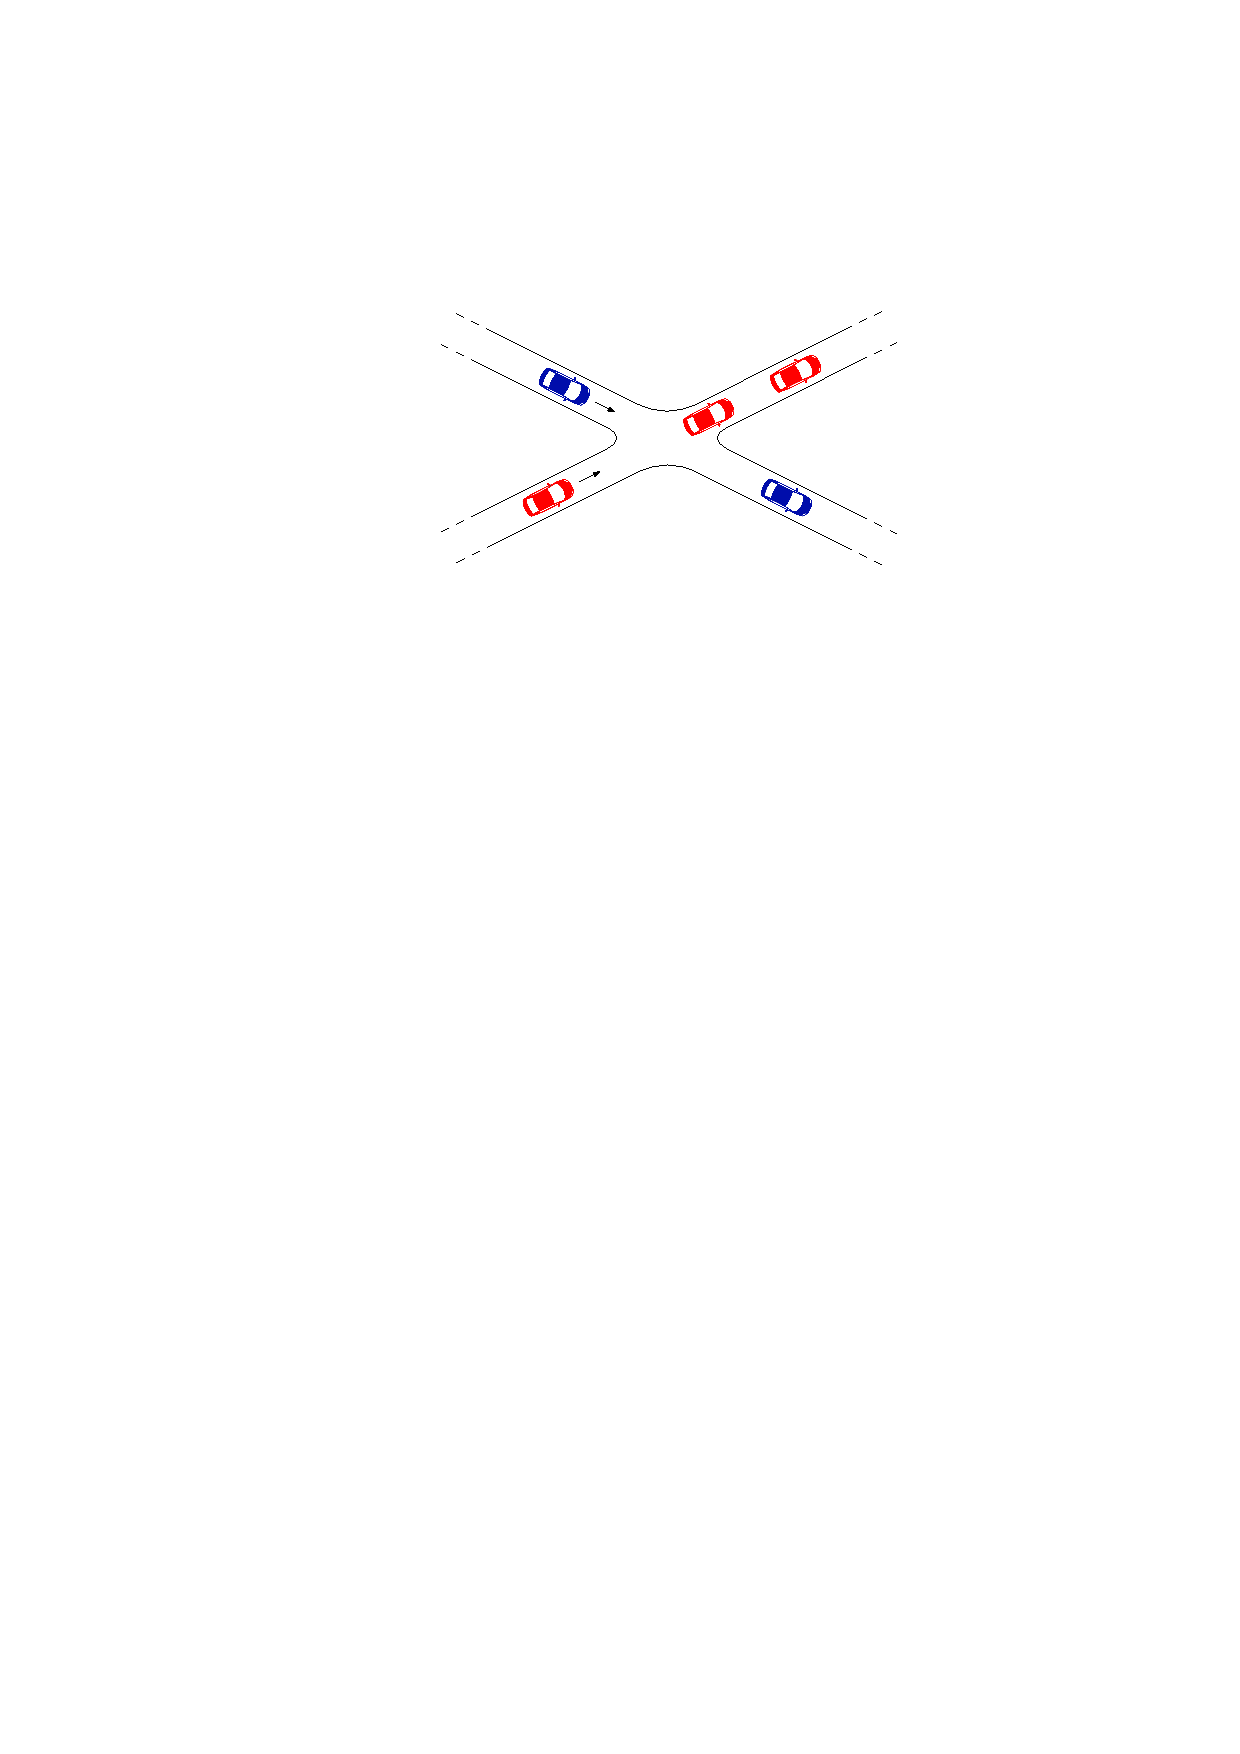
\includegraphics[scale=1]{figures/intersection-nice}
  \caption{Stylized model of a single intersection with two conflicting flows of
    vehicles that are not allowed to turn at the intersection, so we can
    assume---without loss of generality---that vehicles cross the
    intersection in straight lines.}\label{fig:intersection-nice}
\end{figure}

\section{Challenges and opportunities}

\begin{itemize}
  \item Vehicle motion
  \item Crossing sequence
  \item Joint optimization
  \item Patterns in problems $\rightarrow$ use ML
\end{itemize}

\paragraph{Planning crossing sequences.}

In traffic coordination, combinatorial problems arise naturally from ordering
constraints---deciding which vehicle should move first across shared resources
such as intersections, merge areas, or lanes, while taking into account trade-offs
between throughput, fairness, and safety.
%
Traditionally, such problems are resolved by implementing traffic lights or
static rules for yielding.
%
Autonomous connected vehicles provide us with better ways of handling these
conflicts dynamically.

For example, we will focus specifically on the order in which vehicles cross
intersections, which can also be thought of as first grouping vehicles together
and then deciding in which order these groups are allowed to cross the
intersection.
%
Instead of relying on fixed traffic signal phases, we can optimize this decision
for the current traffic situation.
%
Although the number of choices at a single intersection may be relatively
limited, when considering large networks of intersections, the number of
possible crossing sequences grows rapidly.

Furthermore, even when vehicle routes are fixed, such ordering decisions at one
intersection directly influence the arrival process at nearby intersections,
hence these decisions are coupled across the network.
%
Due to this coupling, finding the optimal crossing plan becomes harder when
larger networks are considered, because of the exponential growth of the space
of feasible solutions.
%
This issue is further complicated by the real-time requirement that real traffic
systems impose on the computation time, which motivates the development of fast
computational methods.

\paragraph{Planning vehicle motion.}

We are dealing with the optimization of vehicle trajectories, which is in
general an infinite-dimensional problem.
%
Such problems can be approached in an end-to-end fashion by
\textit{direct transcription} to an equivalent mixed-integer optimization
problem, which can be solved using off-the-shelf solvers. This method can be
used to compute optimal trajectories up to any precision, by choosing a fine
enough time discretization. However, it is exactly this time discretization that
causes prohibitive growth of the number of variables with respect to the size of
the network and the number of vehicles, so this method is only useful for
relatively small problem instances.
%
Moreover, in the context of traffic systems, there are complex constraints and
safety requirements that need to be handled with care.
%
Furthermore, optimization methods would benefit a lot from closed-form
expressions of trajectories, which is in principle possible in some situations,
but the appearance of constraints makes this notoriously difficult in practice.

\paragraph{Joint optimization.}

There are lots of well-understood solution techniques for purely combinatorial
problems.
%
However, in the current context, the combinatorial part of the problem cannot be
considered in isolation. The feasibility and cost of each solution to the
combinatorial part depends in a non-trivial way on the lower-level
continuous-time dynamics and interactions between vehicles.
%
In other words, simultaneously optimizing the combinatorial part and the
continuous-time part, to which we refer as \emph{joint optimization}, poses
major algorithmic challenges.
%
In the literature, heuristics have been studied, often based on the presumption
of decentralized control and communication.
%
However, works in which the combinatorial aspects and the lower-level
continuous-time trajectories are optimized in a unified fashion, in which the
trade-offs that are made can be clearly identified, are scarce in the current
literature.


\section{Related work}

The survey \cite{marianiCoordinationAutonomousVehicles2022} classifies works
mainly on the level of organization. Moreover, apart from vehicle motion around
intersections and other conflict spaces, they also review other interesting
coordination challenges in autonomous traffic management, like smart parking and
ride sharing, which also have significant societal impact.
%
More specifically focused on autonomous intersection management
are~\cite{khayatianSurveyIntersectionManagement2020}, where works are
classified, first on level of organization, but they also consider vehicle
dynamics, conflict detection and scheduling policy.

% studied from wide range of perspectives, methods
% 
The general goal of coordination has been approached from a wide range of
perspectives, which has given rise to diverse concrete problem formulations and
methodologies.
%
The level of organization at which coordination takes place is a very typical
distinguishing feature among existing
works~\cite{marianiCoordinationAutonomousVehicles2022}.
%
A well-known example of \emph{local coordination} is platooning of vehicles, in
which consecutive vehicles on the same lane try to keep close together while
maintaining similar speeds, with the aim of lowering energy consumption by
reducing aerodynamic resistance. It has been shown that platooning can also
result in a more efficient use of
intersections~\cite{miculescuPollingsystemsbasedAutonomousVehicle2016,tachetRevisitingStreetIntersections2016,timmermanPlatoonFormingAlgorithms2021}.
On a larger scale, \emph{global coordination} methods like dynamic route
optimization have been proposed to reduce travel delay for all vehicles in the
network~\cite{rossiRoutingAutonomousVehicles2018}.

% many modeling aspects
%
Apart from the level of organization, coordination problems can have many more
modeling aspects. For example, one may think of heterogeneous vehicles---in
terms of physical differences or functionality---different models of
centralized/decentralized communication between vehicles or with the
infrastructure, under different guarantees on reliability; complex road
topology, curved lanes affecting the maximum safe speed, merging lanes;
implications of mixing human traffic with fully autonomous traffic.


\paragraph{Reservation-based systems.}
% adjacent: auction, bidding, fairness

Instead of an optimization-based perspective, many studies assume that
vehicles communicate with a central intersection controller to reserve time and
space in the conflict area.
%
The major downside of this line of work is that there is generally no precise
control over the trajectories that vehicles take.

The seminal ``Autonomous Intersection Management'' (AIM) model ~\cite{dresnerMultiagentTrafficManagement2004,dresnerMultiagentApproachAutonomous2008} is a
good example of the reservation-based approach.
%
In this framework, vehicles that want to cross the intersection send a request
to the central controller to occupy the cells containing their trajectory for a
certain amount of time. The central controller then decides to grant or deny
these requests based on previously granted requests to facilitate collision-free
trajectories. If a request is denied, the vehicle slows down and attempts to
obtain a new reservation after some timeout.
%
Note that in the original setting, the central controller does not have complete
control over the precise trajectories that vehicles take; each vehicle agent is
more or less able to decide their own optimal speed profile.
%
However, the central controller does impose some constraints on the acceleration
profile inside the intersection to promote throughput.

Various improvements have been made to the original AIM model to improve the
efficiency of the reservation protocol, for example, by having vehicles make
better estimations of their expected time of arrivals to make more accurate
reservations~\cite{auMotionPlanningAlgorithms2010}.
%
Other works consider speed profile recommendations and more fine-grained
prioritization of requests by the intersection
controller~\cite{huangAssessingMobilityEnvironmental2012}.
%
The model has also been extended to networks of intersections, where dynamic
route optimization has been considered as well~\cite{hausknechtAutonomousIntersectionManagement2011}.
%
Later works propose more precise methods for conflict detection than the
original cell-based approach~\cite{levinConflictpointFormulationIntersection2017,liTemporalspatialDimensionExtensionbased2019}.
%
Finally, communication delays play a major role in practice, so a time-aware
extension of AIM has been introduced
in~\cite{khayatianCrossroadsTimeawareApproach2020}.


\paragraph{Optimizing the crossing order.}

Rather than obtaining a crossing order as the result of a sequence of granted
reservation requests, later studies assume that the intersection manager
explicitly optimizes the sequence in which vehicles cross. Most of these works
also address the online setting, accounting for the random arrival of vehicles
over time.
%
In this online setting, the general goal is to find a \emph{schedule} of
crossing times for the current vehicles in the system and update this schedule
every time new arrivals happen, which is the task of the central \emph{crossing
  time scheduling policy}.

% rolling-horizon optimization
A common method to design such a scheduling policy is to use
\emph{rolling-horizon optimization}. For example, taking the AIM model as a
starting point, a paradigm shift from reservation requests to \emph{assignments}
has been proposed in~\cite{levinConflictpointFormulationIntersection2017}, where
a a mixed-integer linear program is solved in a rolling-horizon fashion to
determine the best assignments.
%
A similar approach is described
in~\cite{liTemporalspatialDimensionExtensionbased2019}, but they formulate the
reservation assignment problem as a non-linear optimization problem, which is
solved using a tabu search heuristic.

% bubbles paper
The policy in~\cite{tallapragadaHierarchicaldistributedOptimizedCoordination2017} deals explicitly with the complexity of the crossing order
decisions by defining groups of consecutive vehicles on the same lane. The first
step is to group vehicles into these so-called ``bubbles''. All vehicles in a
bubble are required to cross the intersection together, while maintaining
feasibility with respect to safe trajectories. Next, crossing times are assigned
to bubbles while avoiding collisions. Based on this schedule, a local vehicular
control method~\cite{tallapragadaDistributedControlVehicle2017} is used that guarantees safety to reach the assigned
crossing times.

% miculescu
The work~\cite{miculescuPollingsystemsbasedAutonomousVehicle2016} considers the scheduling policy in the context of a polling
model, where the intersection, its inbound lanes and vehicles are modeled as
server, queues and customers, respectively.
%
Roughly speaking, each time a new vehicle arrives to the system, the crossing
order may be adapted, which is done by simulating a polling policy.
%
They show that if the polling policy satisfies some regularity condition and if
the lanes are long enough, then every updated crossing order is feasible, in the
sense that vehicles in the system that have been assigned a later crossing time
than before are able to decelerate in time to avoid collisions.
%
The generation of continuous-time vehicle trajectories satisfying these crossing
times is handled by numerically solving an optimal control problem.
% timmerman
Building on this work, it has been shown that these trajectories can also be
computed directly using closed-form
expressions~\cite{timmermanPlatoonFormingAlgorithms2021}.

% joshi
Finally, we note that crossing order decisions become particularly interesting
when vehicles with heterogeneous dimensions and dynamics are considered, which
has been investigated in~\cite{joshiTrajectoriesPlatoonformingAlgorithm2025}.
For example, it makes intuitively sense to assign heavy trucks with slow
acceleration/deceleration characteristics to a dedicated lane to avoid
interfering with passenger vehicles that are more agile.

\paragraph{Joint optimization and decomposition methods.}

Finally, we mention some of the few works that have considered the joint
optimization perspective, which has also been called ``signal-vehicle coupled
control (SVCC)''. The prominent theme here is trying to come up with good
approximation algorithms. A central idea in this line of work is trying to
exploit somehow the fact that the problem can be formulated in terms of a
decomposition of the upper-level crossing time scheduling problem and
lower-level problems for generating continuous-time trajectories.

% Hult et al. (offline single intersection with energy objective)
% "An approximate solution to the optimal coordination problem for autonomous
% vehicles at intersections"
The approximation method in~\cite{hultApproximateSolutionOptimal2015} is based
on a bilevel decomposition and considers a quadratic objective involving
velocity as a proxy for energy. The first stage optimizes a schedule of vehicle
crossing times. It uses approximations of each vehicle's contribution to the
total objective as a function of its crossing time. Next, for each vehicle, the
second stage computes an optimal trajectory satisfying the crossing time
schedule, by solving a quadratic program. This approach has been shown to reduce
running times significantly. Unfortunately, the study is limited to a single
intersection and it is assumed that each lane approaching the intersection
contains exactly one vehicle.

% Zhao et al. (bilevel programming model)
The paper~\cite{zhaoBilevelProgrammingModel2021} proposes a trajectory
optimization scheme for a single intersection, also based on the bilevel
decomposition. The lower-level problem is employed to maximize the speed at
which vehicles enter the intersection. Both parts of the problem are solved in an alternating
fashion, each time updating the constraints of the other part based on the
current solution.

\newcolumntype{L}[1]{>{\RaggedRight\hsize=#1\hsize\hspace{0pt}}X}
\begin{table}[t]
\centering
\renewcommand{\arraystretch}{1.2}

\begin{adjustbox}{center}
\scalebox{0.7}{
\begin{tabularx}{2.0\textwidth}{@{} l L{0.7} L{0.45} L{0.35} L{0.45} L{0.7} @{}}
\toprule
\textbf{Ref.} &
\textbf{Paradigm} &
\textbf{Control} &
\textbf{Safety} &
\textbf{Objective} &
\textbf{Notes / Limitations} \\
\midrule
\cite{dresnerMultiagentApproachAutonomous2008} &
Reservation of grid cells for trajectory in intersection &
Multiagent online &
Non-collision &
Delay minimization &
Simplified vehicle model; global heuristic \\

\cite{tallapragadaHierarchicaldistributedOptimizedCoordination2017,tallapragadaDistributedControlVehicle2017} &
Hierarchical control &
Multiagent; online feedback control  &
Failure recovery &
Combination of travel delay and fuel consumption &
Robust to communication failures \\

\cite{levinConflictpointFormulationIntersection2017} &
Mixed-integer linear programming &
Centralized; rolling horizon optimization &
Non-collision &
Travel delay &
Optimization of intersection entry speed  \\

\cite{hultApproximateSolutionOptimal2015,hultTechnicalReportApproximate} &
Approximation algorithm based on bilevel decomposition &
Centralized offline optimization &
Non-collision &
Convex quadratic objective &
Single vehicle per lane \\

\cite{zhaoBilevelProgrammingModel2021} &
Bilevel decomposition with platoon-based scheduling &
Centralized rolling horizon optimization &
Non-collision &
Travel delay &
Optimization of intersection entry speed  \\

\cite{miculescuPollingsystemsbasedAutonomousVehicle2016} &
Provable feasible trajectories under random arrivals  &
Centralized; reoptimization triggered by arrivals &
Non-collision under uncertainty &
Travel delay &
Inspired by polling models; extensive proof of trajectory feasibility  \\

\cite{timmermanPlatoonFormingAlgorithms2021} &
Explicit solution of lower-level optimal control  &
Centralized online &
Non-collision &
Travel delay or minimal acceleration &
No crossing order optimization; performance analysis using polling theory  \\
  
\bottomrule
\end{tabularx}}
\end{adjustbox}
\caption{Comparison of approaches to signal-free intersection management.}
\label{tab:litreview}
\end{table}

\section{Project goals and outline}

% \paragraph{Research goals and questions.}

From the start of this project, the overarching goal has been to develop
tractable optimization models and algorithms for the coordination of autonomous
vehicles at intersections.
%
% is some history appropriate here?
%
In the initial phase, we considered dynamic and stochastic aspects like random
vehicle arrivals. However, after reviewing the current state of the literature,
we realized that there are still many unresolved issues in the deterministic
settings.
%
In the end, this project has been centered around the following two general
goals related to coordination of autonomous vehicles:

% problem-directed goals
\begin{enumerate}[label=\textbullet, leftmargin=3em, rightmargin=4em]
  \item \emph{Develop a simplified yet representative mathematical optimization model
        for coordination of autonomous vehicles in networks of intersections.}

  \item \emph{Understand the inherent algorithmic challenges that complicate joint
        optimization of crossing order and generation of continuous-time
        trajectories.}
\end{enumerate}

Complementary to these problem-driven goals, the work presented in this thesis
has also been inspired by some developments in applying machine learning methods
to combinatorial optimization.
%
% [insert brief discussion of those methods and results]
% refer to appendix for further background
%
\note{[ this needs a little more introduction ]}
Motivated by these recent successes, we also aim to \emph{illustrate the use of
  such machine learning algorithms to obtain heuristics for combinatorial problems arising in the context of coordinating autonomous
  vehicles}.

% research questions: concrete, addressable
To make the above broad goals concrete and addressable, our work has been guided
by the following research questions:

\begin{enumerate}[label=RQ\arabic*:, leftmargin=3em, rightmargin=4em]
  \item How can the autonomous traffic coordination problem with
        collision-avoidance constraints at a single isolated intersection be
        formulated in an optimization framework for multiple autonomous
        vehicles? (modeling)

  \item Under which assumptions can the combinatorial aspect of determining the
        crossing order be considered in isolation? (decomposition)

  \item What is the relative computational complexity of solving the
        combinatorial problem compared to solving the continuous-time trajectory
        optimization, given the crossing order? (complexity)

  \item How to leverage the recent successes in applying machine learning for
        combinatorial optimization to solve the combinatorial problems arising
        in the context of autonomous traffic management? (heuristics)

  \item How to extend the previous questions to a network of multiple connected
        intersections? (scalability)
\end{enumerate}

% concrete goals/research questions:
% - scalable coordination algorithm
% - real-time computational requirements
% - not completely model-free, but partly model-based to exploit apparant structure


\noindent
The contributions of our project can be summarized into three main categories:

\paragraph{(i). Isolating the combinatorial problem.}
Deciding the crossing order of vehicles at intersections is a central challenge
in traffic management. This holds especially for when considering multiple lanes
and intersections.
%
However, after fixing these ordering decisions, the remaining problem is often
much easier to solve. This observation motivates the decomposition of the
trajectory optimization problem into two parts.
%
The upper-level problem determines the times at which vehicles cross the
intersections on their routes, to which we will refer as \emph{crossing times}.
%
Once these are fixed, we solve a set of lower-level problems to find the
corresponding vehicle trajectories satisfying the crossing times.
%
Our first contribution is to show that, under certain conditions, our joint
trajectory optimization problem for vehicles in a network of intersections
decomposes into an upper-level crossing time scheduling problem and a set of
lower-level trajectory optimization problems. We show that feasibility of the
upper-level scheduling problem is completely characterized in terms of a system
of linear inequalities involving the crossing times. This allows us to first
solve the scheduling problem and then generate trajectories for it once we have
the optimal crossing time schedule.

\paragraph{(ii). Learning-based scheduling.}
Our second contribution is an illustration of how machine learning techniques
can be applied to solve scheduling problems in practice, using our crossing time
scheduling problem as a case study.
%
Many practical instances of combinatorial problems contain structure that
classic solutions techniques try to exploit, e.g., by defining smart heuristics
based on human intuition and experience.
%
A recent trend in the literature has been to aim for automation of this manual
endeavor, for example by formulating parametric sequence models to capture the
conditional probability of optimal solutions, given a problem instance.
%
Specifically, we recognize that the solution of the crossing time scheduling
problem can be interpreted as a sequence of decisions.
%
Instead of manually trying to develop good heuristics and algorithms, we try to
learn what optimal solutions are, by treating it as a learning task on
sequences.
%
As has been noted before, we confirm that the order of evaluation during
inference matters a lot for the final solution quality.

\paragraph{(iii). Coordination across multiple intersections.}
We show a way to extend isolated intersection coordination to multi-intersection
networks. We show under which assumptions this problem can still be formulated
as a scheduling problem, which turns out to be an extension of the classical job
shop scheduling problem.
%
In this setting, feasibility of trajectories deserves special attention.

\paragraph{Outline.}

In Chapter~\ref{chap:single}, we consider a simple model of a single
intersection, like the example above. After discussing the decomposition method,
we present some classical solutions methods to solve the crossing time
scheduling problem.
%
We explain how the problem can be treated as a learning problem in
Chapter~\ref{chap:single-learning}.
%
In order to generalize to a network of intersections, we need to give a precise
characterization of the feasibility of trajectories in lanes of finite length,
which is done in Chapter~\ref{chap:network}.
%
The resulting scheduling problem is then subjected to a learning algorithm in
Chapter~\ref{chap:network-learning}.
%
We provide some general discussion and pointers for further research in
Chapter~\ref{chap:conclusion}.

\section{Intro bits and pieces}

% broad problem:
% - why intersections matter in traffic coordination
% - why coordination is interesting

% simpflified model as a tractable starting point
% assumptions:
% - two lanes
% - perpendicular
% - no turning
% - no overtaking
% - homogeneous vehicles (same dimensions and dynamics)
% - no randomness
%  - fixed

% optimization objective:
%   - energy consumption -> very desirable on top of delay, but makes analysis difficult
%   - travel delay -> essential, enables problem simplification (decomposition)

% mathematical punchline:
% - first, it becomes a trajectory optimization problem (optimal control)
%   - can be solved directly
% - next, we turn it into a very simple scheduling (when) / sequencing (only order) problem

% preview of results:
% - mention direct transcription
% - main takeaway: bilevel decomposition
% - branch-and-cut solution
%   - problem structure yields cutting planes
%   - analye performance improvement
% - optionally, mention local search

Efficient coordination of vehicle motion at intersections has always been a
central challenge in traffic management. Intersections are natural bottlenecks
where safety requirements and efficiency objectives are directly in conflict,
calling upon systems of law or technology to avoid chaos.
%
With the advent of autonomous vehicles and reliable wireless communication
technologies, there is increasing potential to replace traditional traffic
signal-based approaches with coordinated trajectory planning methods.

Our literature review clearly shows that previous works have approached
coordination of autonomous vehicles from a wide range of perspectives and with
varying degrees of model complexity.
%
Furthermore, we highlighted some fundamental computational challenges that are
still unresolved in the literature.
%
Specifically, the joint optimization of crossing order and continuous-time
vehicle trajectories has received relatively little attention.
%
In order to better understand this issue and to enable precise analytical
results, we propose to study a stylized single intersection model.

\paragraph{Optimal control.}

The decision variables in this kind of problem represent the individual
vehicle's trajectories, which are functions of time.
%
The study of optimizing over functions traces back to the calculus of
variations, which has evolved into the modern theory of optimal
control~\cite{liberzonCalculusVariationsOptimal}.
%
The latest manifestation of this line of research is found within the roots of
the popular field of reinforcement learning, which grew out of the dynamic
programming approach to optimal
control~\cite{bellmanDynamicProgramming1984,bertsekas2012dynamic,putermanMarkovDecisionProcesses2009,suttonReinforcementLearningIntroduction2018}.


% \microtypesetup{deactivate}
% \part*{\hspace*{-0.8em}\textsc{Part I}\\[0.6em] Isolated Intersection\\[3em]
%        \centering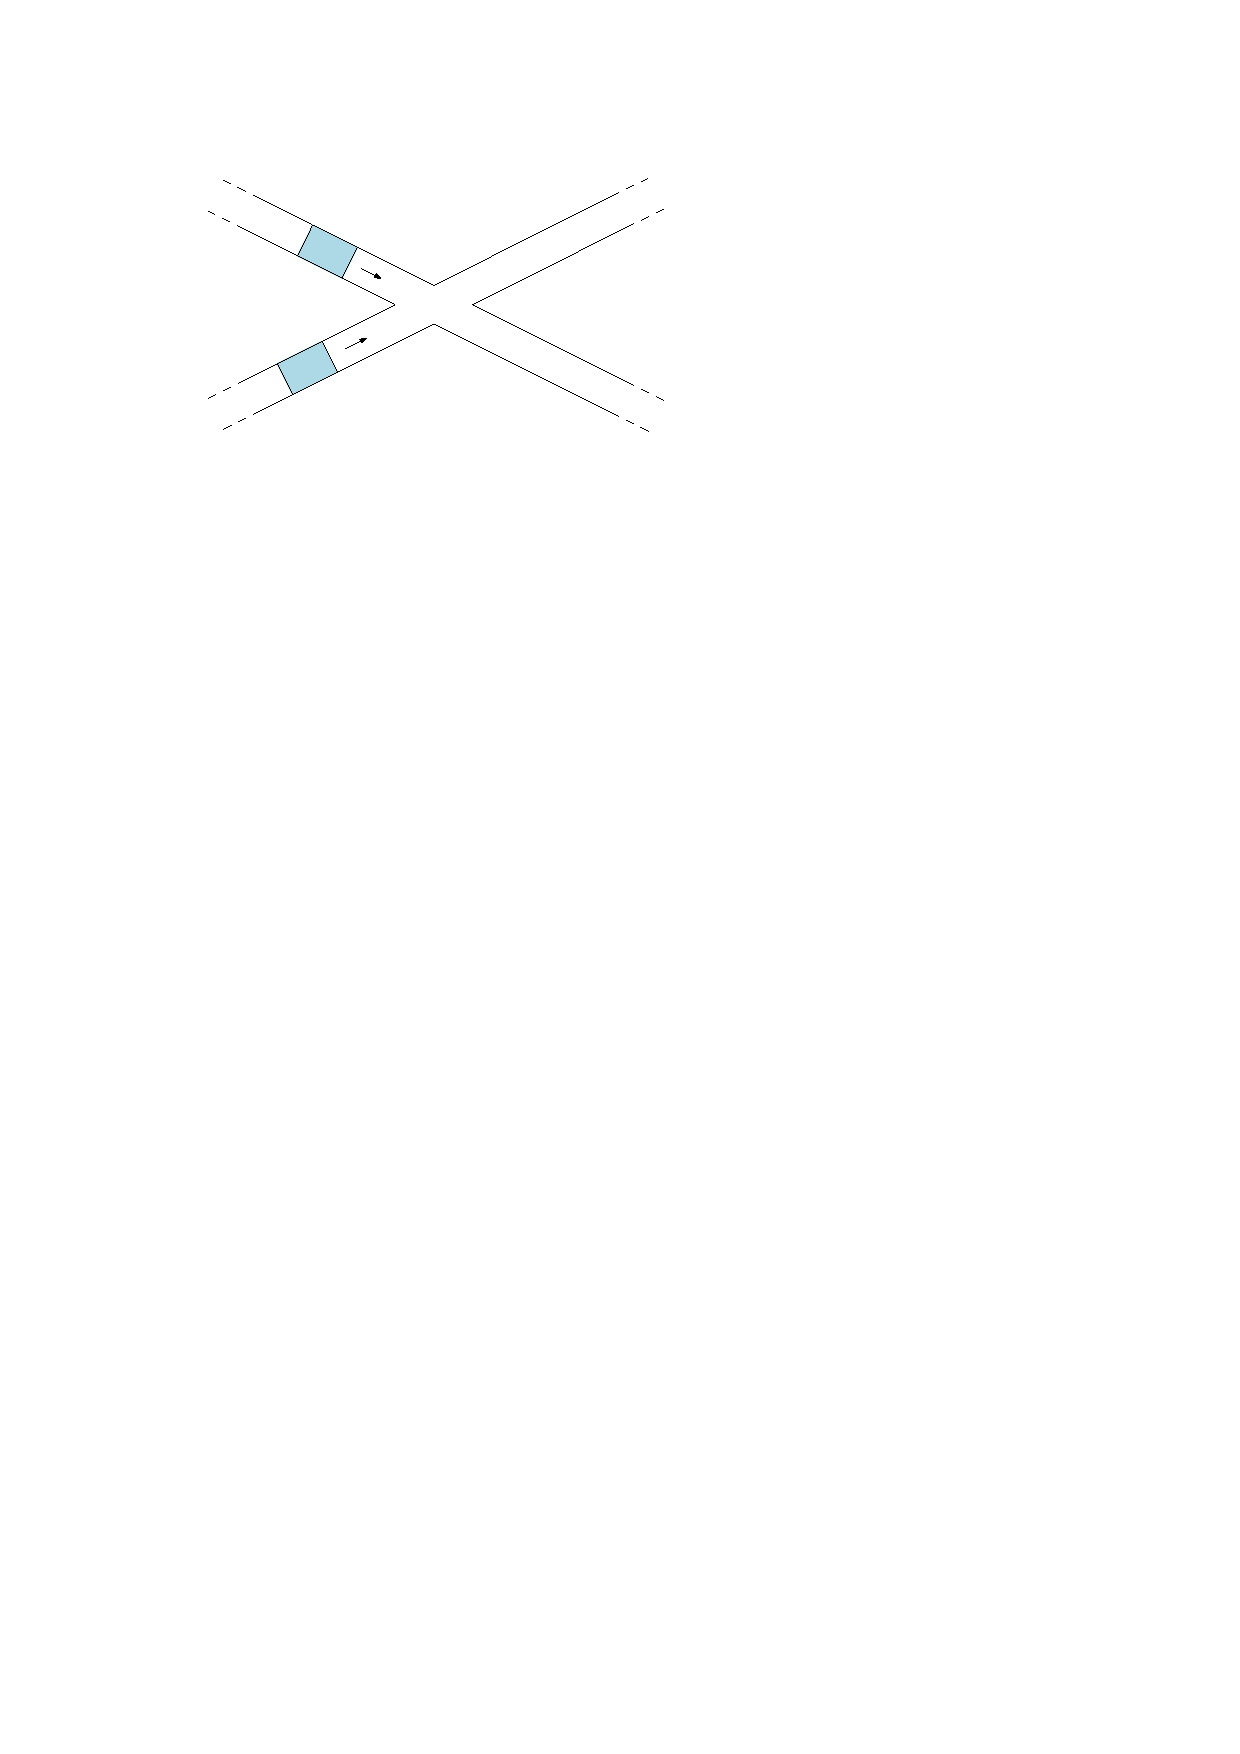
\includegraphics[scale=1]{figures/intersection-non-axis-aligned}}
% \microtypesetup{activate}
% \addcontentsline{toc}{part}{Part I \;--\; Isolated Intersection}


\chapter{Motion planning in fully autonomous intersections}\label{chap:single}

% general optimization goals
Given the controlled environment sketched in the introduction, this chapter will
further detail our mathematical optimization approach to traffic management of
autonomous vehicles.

\paragraph{Autonomous intersection model.}
In~\Cref{sec:intersection-model}, we model a single isolated intersection in which
vehicles, equipped with perfect communication and steering capabilities, operate
under the supervision of a central traffic manager.
%
The model is based on the essential trade-offs inherent to all transportation
systems. Specifically, the model is general enough to capture the following
three fundamental and conflicting objectives.
%
\begin{itemize}
  \item \emph{Guaranteeing safety} remains the primary design requirement in any
        transportation system, has highest priority and is almost non-negotiable
        in practice. We say \emph{almost}, because real systems are too complex
        to strive for zero chance of failure. In mathematical models, there is
        no such excuse. In our model, safety is defined simply as the absence of
        vehicle collisions.

  \item \emph{Minimization of delay} is one of the central measures of efficiency and
        service quality. It is directly related\footnote{In stylized queueing models of traffic, the relationship between these quantities is given by Little's law.} to the \emph{capacity} of the
        system---in terms of the maximum number of vehicles---and to the
        \emph{throughput}---in terms of the number of completed journeys or trips per
        second.

  \item \emph{Energy efficiency}, which contributes both to sustainability goals
        and to the reduction of economic operational costs, is a desirable
        secondary goal. It also indirectly contributes to passenger comfort,
        because energy minimization results in smooth trajectories with
        controlled acceleration and deceleration.
\end{itemize}


\paragraph{Trajectory optimization.}
The task of safely and efficiently coordinating the motion of autonomous vehicles
through our single-intersection model, can be formulated mathematically as 
\emph{trajectory optimization}, which is precisely defined in
Section~\ref{sec:motion-planning}.
% direct transcription
Perhaps the most natural way of solving this kind of problems depends of
discretization of the time domain.
%
In Section~\ref{sec:direct-transcription}, we will illustrate a widely
applicable method known as \emph{direct
  transcription},
which is relatively straightforward to implement and guarantees to find an
optimal solution.
%
The price we pay for the generality of this method is the fact that its running
time scales very poorly, in the sense that finding an optimal solution becomes
intractable relatively quickly, when considering larger numbers of vehicles in
the system or making the time discretization finer.
%
This motivates the development of more specialized algorithms that leverage
the structure of the particular problem at hand.

\paragraph{``Who goes first?''}
We conclude this chapter by discussing the most salient structural property of
the trajectory optimization problem, which is a direct consequence of
requirements on safety.
%
Indeed, in order to avoid collision between vehicles from opposing lanes, we
need to fix a particular \emph{crossing order} among the vehicles in the system.
%
This observation leads to the following natural reformulation of the problem.
First, we allocate each vehicle to an \emph{occupancy time slot}, being the time
reserved for this vehicle to cross the intersection. Second, we try to assign
each vehicle a trajectory satisfying its reservation.

It is natural to ask to what extent this decomposition simplifies the
formulation by facilitating a two-step procedure: can we first optimize the
crossing order as a separate stage, and then compute the corresponding vehicle
trajectories afterwards?
%
In general, the answer is negative. Nevertheless, the decomposition serves as a
useful conceptual tool that can guide algorithm development, so we introduce the
decomposition mathematically in~\Cref{sec:bilevel} and we discuss one
interesting example of an approximation algorithm from the literature
in~\Cref{sec:approx-algos}.

\paragraph{Delay minimization.}

Mathematicians are naturally inclined to seek the most general possible
formulation. In~\Cref{sec:delay-minimization}, however, we deliberately focus on
a more specific setting that captures the essential features of the problem,
while enabling us to take full advantage of the decomposition.
%
We make the following two assumptions:
\begin{itemize}
  \item Vehicles drive, and remain driving, at \emph{full speed} from the
        moment they first enter the intersection area.
  \item The optimization objective is stated purely in terms of \emph{travel delay};
        we do not take into account any further kind of property related to the
        smoothness or \emph{shape} of the vehicles trajectories.
\end{itemize}
%
\emph{Under these assumption, the decomposition is proper}. Consequently, the
infinite-dimensional trajectory optimization problem reduces to a
finite-dimensional \emph{scheduling problem}, in terms of finding feasible sets
of intersection occupancy time slots, while minimizing the total travel delay.
%
Subsequent chapters are devoted to solving this reduced problem.

\section{The single intersection model}\label{sec:intersection-model}

% model assumption to make analysis tractable
To keep the model simple, we restrict our attention to intersections of
single-lane roads on which vehicles are traveling without turning maneuvers or
overtaking.
%
All vehicles are assumed to be homogeneous, sharing identical dimensions and
dynamics, such that their motion can be modeled uniformly.
%
A central controller determines the acceleration, and thus the speed, of each
vehicle, under the assumption of perfect communication.
%
Moreover, we do not consider randomness in arrivals or dynamics, so we assume
that each vehicle's initial state is known precisely such that the system
evolves deterministically as a function of the acceleration control inputs.

We start by defining the geometry of the intersection and the vehicles and
analyze the resulting conflict-free joint positions of all the vehicles in the
system.
%
After that, we introduce the dynamics of the system and define objective
functions.
%
The ingredients here will be used to formulate the trajectory optimization
problem in the next section.

\subsection{Collision-free vehicle positions}\label{sec:valid-configs}
%
We model each vehicle $i$ in the plane as some rigid body $\mathcal{B}_{i}$
traveling along some straight line $r(i)$, to which we will refer as the
vehicle's \emph{route}.
%
We will assume that vehicles always stay on their route and thus do not make
turning maneuvers.
%
Therefore, the longitudinal position of a vehicle along its route can be
represented by some scalar $x_{i} \in \mathbb{R}$.
%
For simplicity, we use a rectangular vehicle geometry, so each $\mathcal{B}_{i}$
is a translated rectangle of width $W_{i}$ and length $L_{i}$. For technical
convenience, we assume this rectangle is an \emph{open} set. We write
$\mathcal{B}_{i}(x_{i})$ to denote the corresponding translated rigid body in
the plane, where $x_{i}$ corresponds to the location of the front bumper; the
rear bumper position is then $x_{i} - L_{i}$.
%
We allow multiple routes to cross in a single point. Of course, this causes some
joint vehicle positions to be invalid, because they would correspond to
collisions.
%
Before we allow arbitrary numbers of vehicles to have the same route, we briefly
investigate the safe configurations of two vehicles, each on its own route.

\begin{figure}[b]
  \centering
  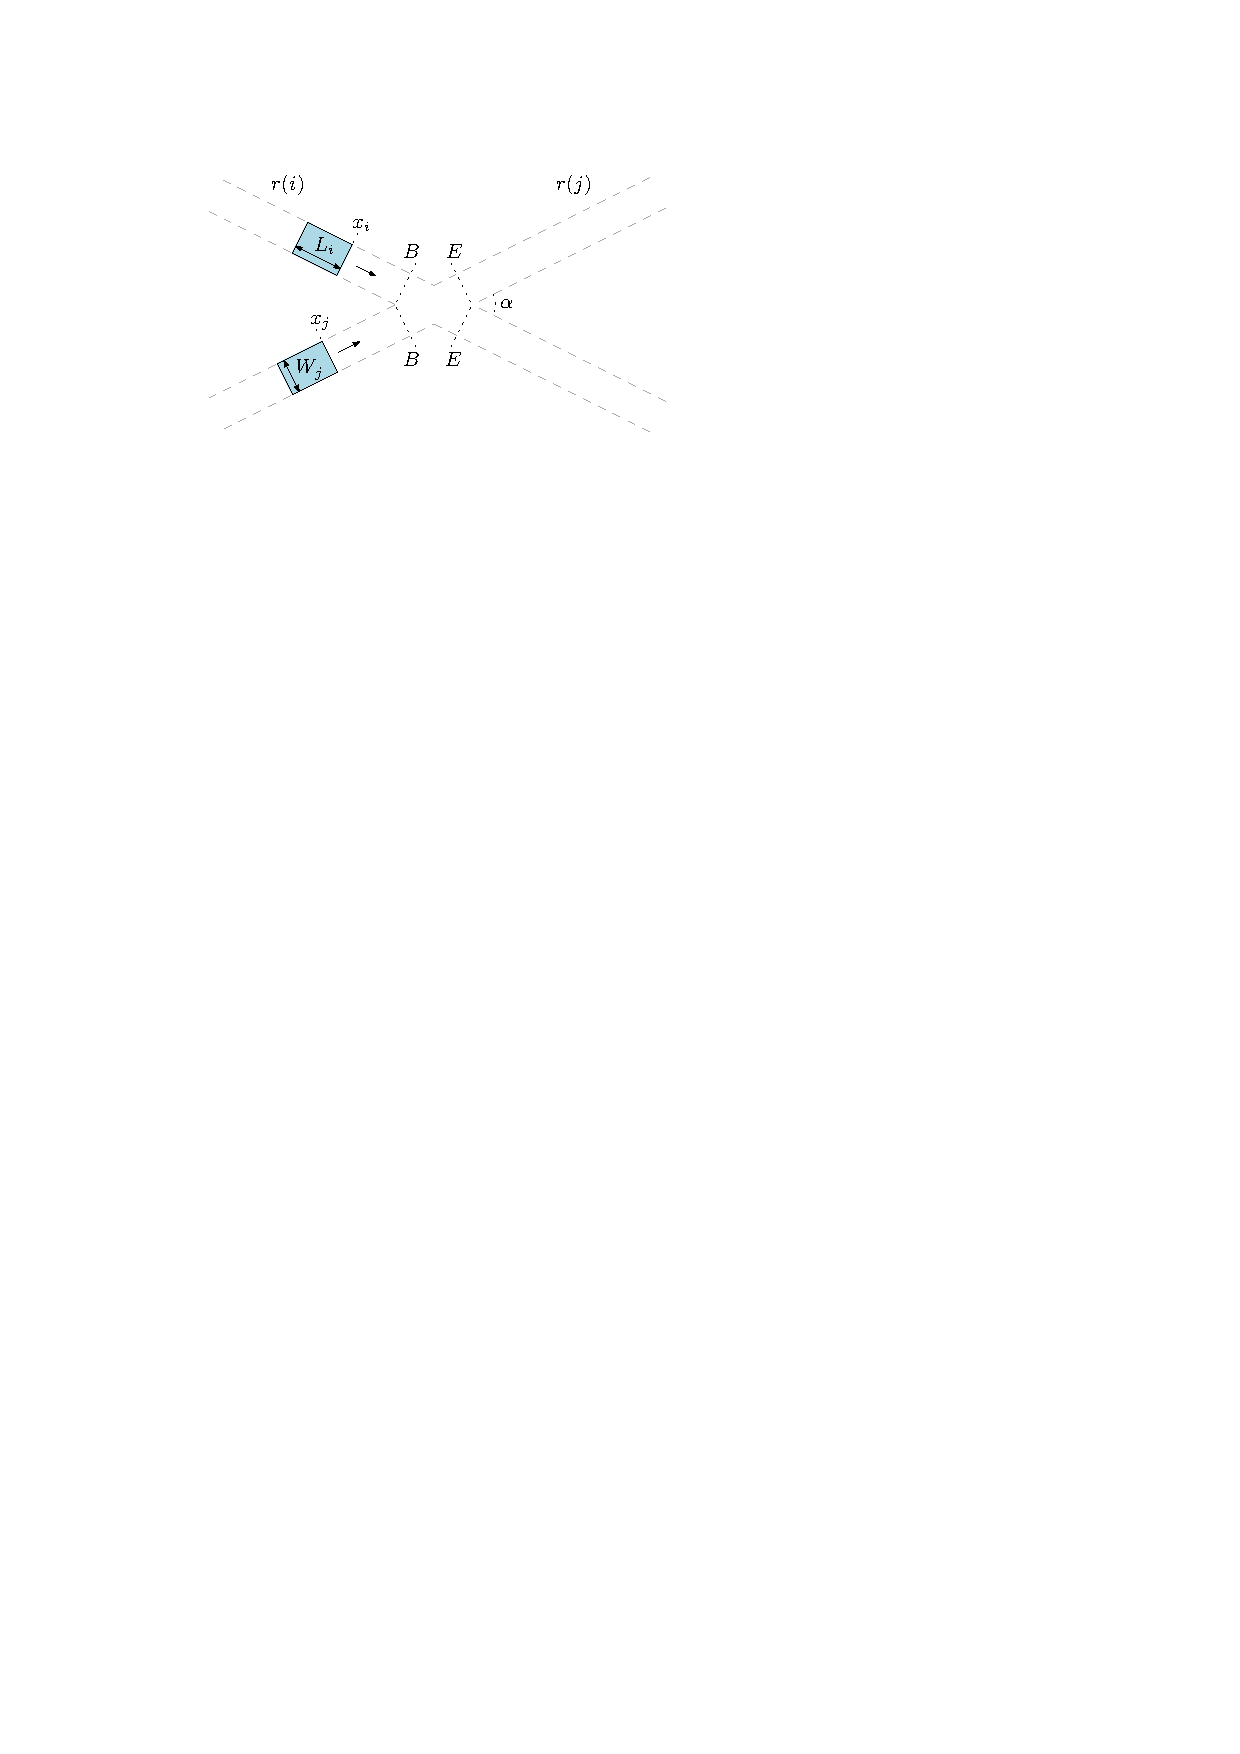
\includegraphics[scale=1.1]{figures/intersection-non-axis-aligned-annotated}
  \caption{Example of two vehicle routes intersecting at some angle $\alpha$. The
    indicated positions $x_{i} = B$ and $x_{i} = E$ for each vehicle $i$ are
    chosen such that whenever the vehicle position $x_{i}$ satisfies either
    $x_{i} \leq B$ or $x_{i} - L_{i} \geq E$, then the intersection area is not
    occupied by this vehicle at all and the other vehicle can take any position
    without causing a collision.}%
  \label{fig:intersection-non-axis-aligned}
\end{figure}

Consider two routes intersecting at some angle $\alpha$, as illustrated in
Figure~\ref{fig:intersection-non-axis-aligned}, each with a single vehicle on
it. Let these vehicles be denoted as $i$ and $j$.
%
We can try to characterize the set $\mathcal{X}_{ij} \subset \mathbb{R}^{2}$ of
configurations $(x_{i}, x_{j})$ for which these two vehicles are not in
a collision, in the sense that their corresponding translated open rigid bodies
do not intersect.
%
In general, the set of all safe configurations is defined as
\begin{align}
  \label{eq:3}
  \mathcal{X}_{ij} := \{ (x_{i}, x_{j}) \in \mathbb{R}^{2} : \mathcal{B}_{i}(x_{i}) \cap \mathcal{B}_{j}(x_{j}) = \varnothing \} ,
\end{align}
which is a closed set.
%
However, it is often easier to take the opposite perspective, by characterizing
the set of conflicting configurations $\mathcal{X}_{ij}^{C}$, which is open.
% \comment{Nice, C for conflict and for complement!}

% discuss rectangular subset of configuration space
%
In the situation with two routes, we fix two reference positions $B$ and $E$ on
each route, delimiting the intersection area as shown in
Figure~\ref{fig:intersection-non-axis-aligned}.
%
These positions are chosen such that whenever $x_{i} \leq B$ or
$x_{i} - L_{i} \geq E$, it is clear that vehicle $i$ does not occupy the
intersection, so the other vehicle $j$ is free to take any position
$x_{j} \in \mathbb{R}$.
%
Thus, we obtain the following conservative approximation of the set of conflicting
configurations:
\begin{align}\label{eq:conf-space-approx}
  (B,E + L_{i}) \times (B, E + L_{j}) \supseteq \mathcal{X}_{ij}^{C} ,
\end{align}
where $(a, b) := \{ c\in \mathbb{R} : a < c < b\}$ denote the open interval and
$\times$ is the cartesian product.
%
Of course, the set of feasible configurations is generally a little larger and
depends on the angle $\alpha$ of intersection, as illustrated by the three examples
in Figure~\ref{fig:intersection-config-spaces}.
%
In the right-most example, where the intersections make a right angle
$\alpha = \pi/2$, observe that there is actually equality in~\eqref{eq:conf-space-approx}.
%
To keep the presentation simple, we will make the following assumptions.

\begin{assump}
  All vehicles share the same vehicle geometry, i.e, $L_{i} \equiv L$ and
  $W_{i} \equiv W$. As a shorthand of the vehicle positions that correspond to
  occupying the intersection area, we will write $\mathcal{E} := (B, E + L)$.
  % 
  This enables us to model any number of intersecting routes, as long as we can
  assume that $\mathcal{E}^2 = \mathcal{E} \times \mathcal{E}$ provides a safe
  way to approximate all intersection-occupying vehicle positions.
\end{assump}

\begin{figure}[b]
  \centering
  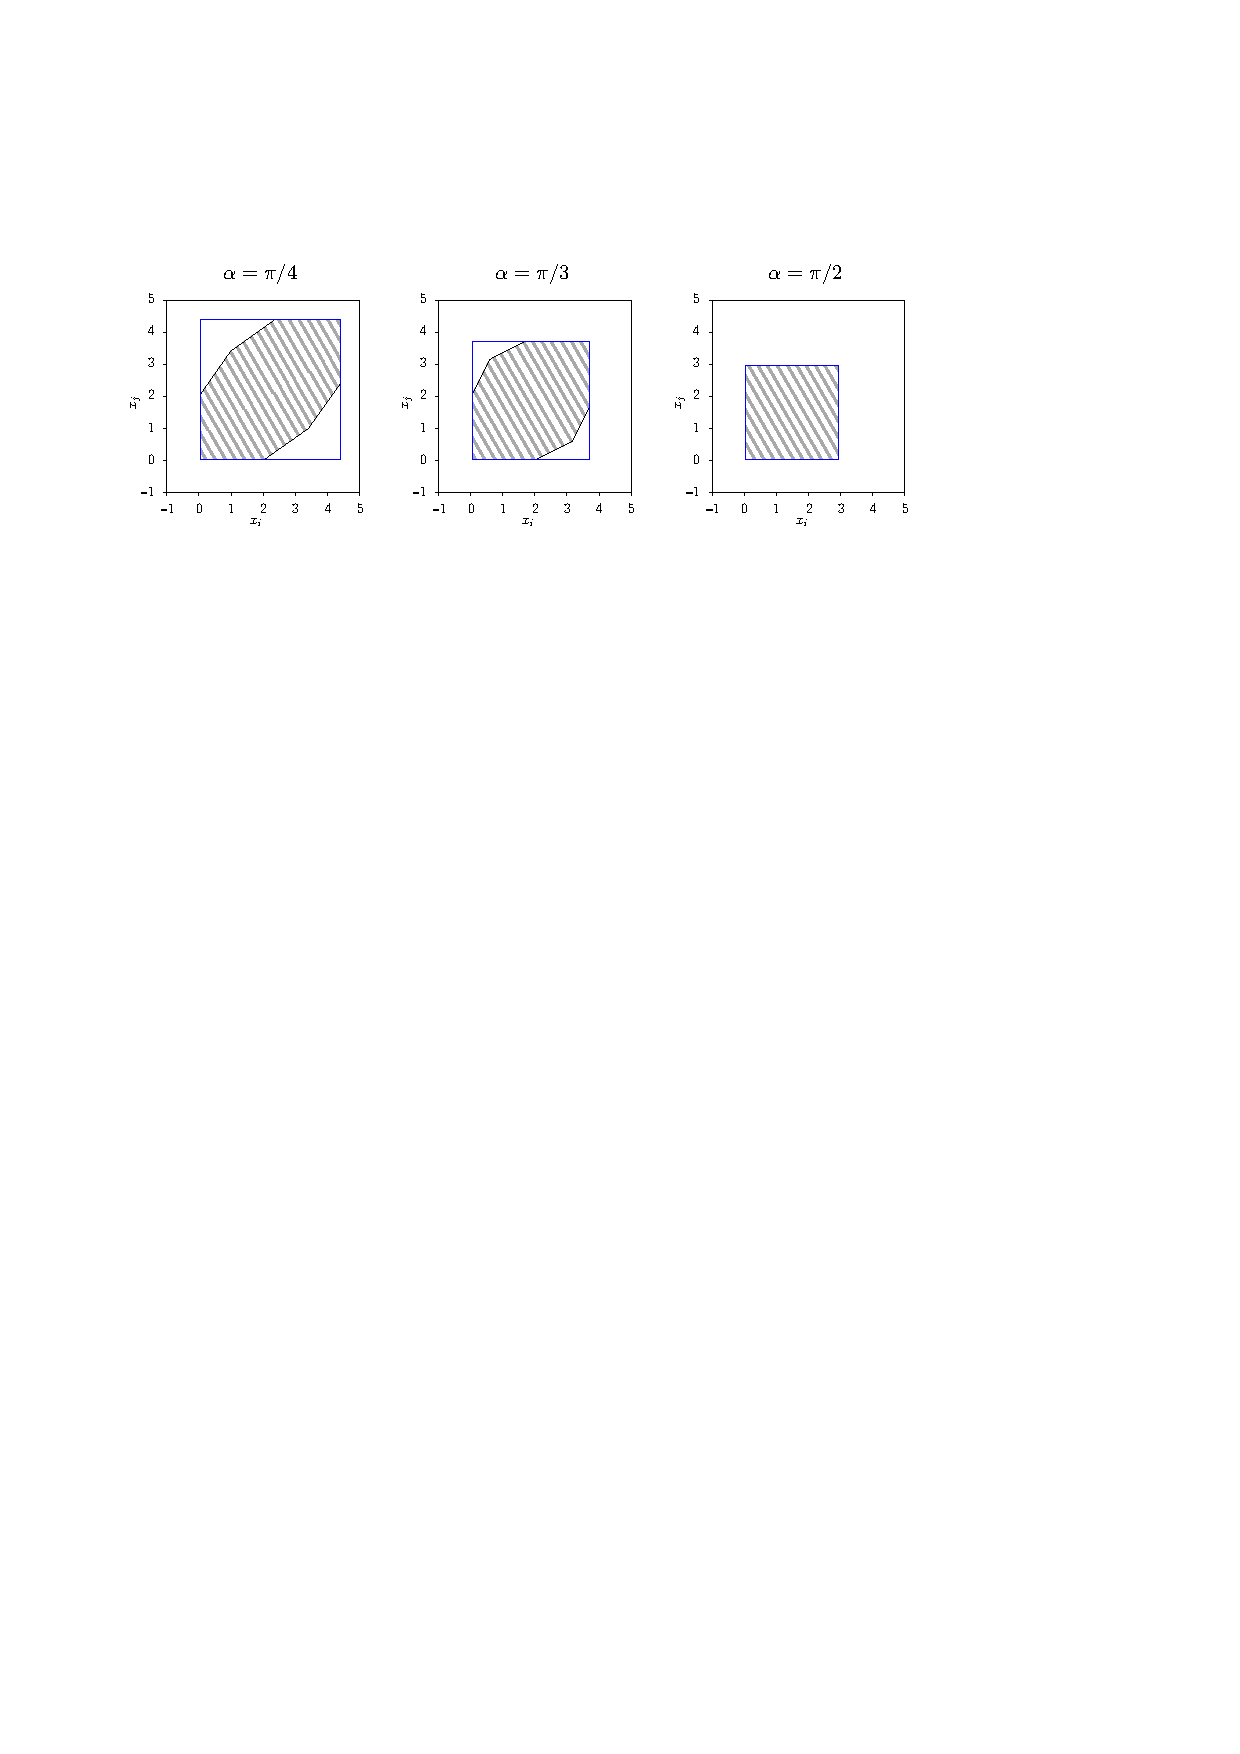
\includegraphics[scale=1]{figures/intersection-config-spaces}
  \caption{For three different intersection angles and fixed vehicle dimensions
    $W_{i} = W_{j} = 1$ and $L_{i} = L_{j} = 2$, we plotted the region
    $\mathcal{X}_{ij}^{C}$ in configuration space corresponding to collisions as
    the area marked in grey. The blue square shows the approximation of
    $\mathcal{X}_{ij}^C$ given by the left-hand side of~\eqref{eq:conf-space-approx}. Because we assume a
    rectangular vehicle geometry, these figures are relatively straightforward
    to compute, which we briefly explain in
    Appendix~\ref{app:configuration-space}.}%
  \label{fig:intersection-config-spaces}
\end{figure}

% collision-avoidance in routes
% \paragraph{Multiple vehicles.}
Let us now proceed to considering arbitrary numbers of vehicles. We will use the
following notation to identify routes and the vehicles associated with them.

\begin{define}
Let the routes be identified by indices $\mathcal{R} := \{1, \dots, R\}$. Let
$n_{r}$ denote the number of vehicles following route $r$, and let
$N := n_1 + \dots + n_R$ denote the total number of vehicles in the system, for
which we have the set of vehicle indices
\begin{align}
  \mathcal{N} := \{ (r, k) : k \in \{1, \dots, n_{r}\}, r \in \mathcal{R}\} .
\end{align}
Given vehicle index $i = (r, k) \in \mathcal{N}$, we use
the auxiliary notation $r(i) = r$ and $k(i) = k$.
%
To identify the set of vehicles on route $r$, we use the shorthand notation
\begin{align}
  \mathcal{N}_{r} := \{ i \in \mathcal{N} : r(i) = r \} .
\end{align}
Define the set of unordered \emph{conflict} pairs
\begin{align}
  \mathcal{D} := \{ \{i,j\} \in \mathcal{N} : r(i) \neq r(j) \} ,
\end{align}
and the set of \emph{consecutive} or \emph{conjunctive} pairs
\begin{align}
  \mathcal{C} := \{ (i,j) \in \mathcal{N} : r(i) = r(j) \text{ and } k(i) + 1 = k(j) \} .
\end{align}
\end{define}

\pagebreak[3]
% disjunctions (conflicts)
Recall that $\mathcal{E}$ denotes the interval of intersection-occupying
positions for each vehicle in the system. Therefore, imposing the \emph{safe
  crossing constraints}
\begin{align}\label{eq:safe-crossing}
  (x_{i}, x_{j}) \notin \mathcal{E}^{2} 
\end{align}
for each conflict $\{i,j\} \in \mathcal{D}$ guarantees the absense of
collisions between vehicles from conflicting routes.
% conjunctions (vehicle following)
Next, we prevent collisions between consecutive vehicles by further imposing
the \textit{safe headway constraints}
\begin{align}
  \label{eq:follow_constraints}
  x_{i} - x_{j} \geq L ,
\end{align}
for each conjunctive pair $(i, j) \in \mathcal{C}$. Obviously, these constraints
restrict vehicles from overtaking each other, so their initial relative order is
always maintained. In other words, $(i,j) \in \mathcal{C}$ means that $i$ crosses
the intersection before $j$.


\subsection{Motion dynamics}\label{sec:dynamics}

Now that we established the static features of the model, we will introduce the
dynamical behavior of the system. In other words, we describe how the position
of vehicles are allowed change as a function of time.
%
Let $x_{i}(t)$ denote the position of vehicle $i$ at time $t$ and let
$\dot{x}_{i}(t)$ and $\ddot{x}_{i}(t)$ denote its speed and acceleration,
respectively.
%
Consider the bounds
\begin{subequations}\label{eq:vehicle-dynamics}
\begin{alignat}{3}
  0         & \leq & \; \dot{x}_{i}(t)  & \leq && \; \bar{v}  , \label{eq:speed-constr} \\
  {-\omega} & \leq & \; \ddot{x}_{i}(t) & \leq && \; \bar{\omega} ,
\end{alignat}
\end{subequations}
for some positive $\bar{v}, \omega, \bar{\omega} > 0$.
%
Given a pair of initial position and velocity $s_{i} = (x_{i}^{0}, v_{i}^{0})$,
we write $x_{i} \in D(s_{i})$ if and only if the trajectory $x_{i}$ has
$(x_{i}(0), \dot{x}_{i}(0)) = s_{i}$ and satisfies~\eqref{eq:vehicle-dynamics}.

% initial state, final time
Let the joint initial state of the system be denoted by
\begin{align*}
  s := \{s_{i} = (x_{i}^{0}, v_{i}^{0}) : i \in \mathcal{N} \} .
\end{align*}
%
The existence of trajectories
satisfying~\eqref{eq:safe-crossing},\eqref{eq:follow_constraints}
and~\eqref{eq:vehicle-dynamics} generally depends on the initial state $s$ of
vehicles in some non-trivial manner.
%
To give a rough idea, we derive some simple sufficient conditions.
% feasibility assumption
We exclude initial collisions at time $t=0$ by requiring
\begin{align}\label{eq:initially-safe-assumption}
 x_{i}^{0} - x_{j}^{0} \geq L \quad \text{ for all } \quad  (i,j) \in \mathcal{C} .
\end{align}
%
% full acc/dec times and distances
%
Next, observe that the bounds on speed and acceleration imply that it takes at
least $\bar{v}/\omega$ time to fully decelerate from full speed, during which the
vehicle has traveled a distance of $\bar{v}^2/(2\omega)$. Similarly, a full
acceleration from a stop takes $\bar{v}/\bar{\omega}$ time and
$\bar{v}^2/(2\bar{\omega})$ distance.
%
Therefore, by assuming that each vehicle starts at full speed
$v_{i}^{0} = \bar{v}$ and by imposing a minimum distance to the start of the
intersection
\begin{align}\label{eq:initial-safe-stopping-assumption}
  x_{(r,1)}^{0} \leq B - \bar{v}^2/(2\omega) - \bar{v}^2/(2\bar{\omega}),
\end{align}
for each first vehicle on every route
$r \in \mathcal{R}$, we ensure that there is enough room for all vehicles to
come to a full stop. Even further, there is still enough distance for a full
acceleration to reach full speed while crossing the intersection.
%
From now, we will assume:

\begin{assump}\label{assump:feasible}
  The initial states $s=\{s_i = (x_i^0,v_i^0) : i \in \mathcal{N} \}$
  satisfy~\eqref{eq:initially-safe-assumption}
  and~\eqref{eq:initial-safe-stopping-assumption}.
\end{assump}


% cost functional
\subsection{Performance criteria}\label{sec:criteria}
We now present some possible ways of measuring how desirable an individual
vehicle trajectory $x_{i}(t)$ is, by defining a cost functional $J(x_{i})$ that
we aim to minimize.
%
For example, consider the following parametric cost functional
\begin{align}
  J_{\alpha,\beta}(x_{i}) = \int_{0}^{t_{f}} \alpha x_{i}(t) + \beta |\ddot{x}_{i}(t)| \diff t .
\end{align}
%
First of all, note that the absolute value of the acceleration is often used as
a proxy for energy consumption, so $\beta > 0$ is generally desirable.
%
% \comment{There are nice physics arguments why one proxy is preferred over the other, but we just ignore this.}
%
Minimizing energy is in direct conflict with our other main goal, which is to
reach the intersection in some reasonable amount of time. However, we have not
yet explicitly encoded this.
%
We will explicitly add this goal later, but for now, it is possible to achieve a
similar effect by setting $\alpha < 0$, which may be interpreted as rewarding
trajectories that ``move forward fast'' and is thus a natural choice if we want
to promote overall throughput of the system.
%
In some sense, minimizing $J_{\alpha,\beta}$ with $\alpha = -1$ and $\beta = 0$ can be interpreted
as modeling the kind of \emph{hasty} human driving behavior we are all too familiar with.

To provide another example of a sensible criterion, consider cost functionals of
the form
\begin{align}\label{eq:energy-objective}
  J_{v_{d}}(x_{i}) = \int_{0}^{t_{f}} {(v_{d} - \dot{x}_{i}(t))}^{2} + {(\ddot{x}_{i}(t))}^{2} \diff t ,
\end{align}
where $v_{d} > 0$ is some reference velocity. This objective can be interpreted
as trying to maintain a velocity close to $v_{d}$, while simultaneously
minimizing the square of acceleration as proxy of energy consumption.
%
Furthermore, note that the occurance of $(\cdot)^2$ is generally prefered over
$|\cdot|$ in practical applications, because the former has nicer smoothness
properties; the absolute value is not differentiable at zero.

\subsection{Trajectory optimization}\label{sec:motion-planning}

Given the above three main ingredients, we are now ready to formulate the
trajectory optimization problem in terms of finding vehicle trajectories $x_i$
that are
\begin{samepage}
\begin{description}[leftmargin=\parindent,labelindent=\parindent,labelwidth=\widthof{\bfseries collision-free }]
  \item[safe] $\rightarrow$ $x_i$ satisfy the safety constraints of
        Section~\ref{sec:valid-configs} at all times;
  \item[admissible] $\rightarrow$ $x_i$ satisfy the dynamic motion constraints of
        Section~\ref{sec:dynamics};
  \item[efficient] $\rightarrow$ $x_i$ are optimal w.r.t.\ some criterium of
        Section~\ref{sec:criteria}.
\end{description}
\end{samepage}
%
Assume the system parameters
$(L,\mathcal{E}, \bar{v}, \omega, \bar{\omega}, t_{f})$ to be fixed, where
$t_f > 0$ denotes some final simulation time.
%
We write $x := \{ x_{i} : i \in \mathcal{N} \}$ to denote the \emph{joint position}
of vehicles, and $x(t)$ the corresponding \emph{joint trajectory}. Consider the
following optimization problem over $x$.

\begin{mdframed}
\vspace{-\abovedisplayskip}
\begin{alignat}{3}\label{eq:T}
  J(s) := \min_{x} \;\, & \sum_{i \in \mathcal{N}} J(x_{i}) \tag{T} \\
  \text{such that } \; & x_{i} \in D(s_{i}) && \quad \text{ for all } i \in \mathcal{N} , \tag{T.1} \label{eq:T1} \\
  % \text{such that } \; & (x_{i}(0), \dot{x}_{i}(0)) = (x_{i}^{0}, v_{i}^{0}) && \quad \text{ for all } i \in \mathcal{N} ; \nonumber \\
           % \omit\rlap{and for all $t \in [0,t_{f}]$:} \notag \\
           % & \dot{x}_{i}(t) \in [0, \bar{v}]  && \quad \text{ for all } i \in \mathcal{N} , \nonumber \\
           % & \ddot{x}_{i}(t) \in [{-\omega}, \bar{\omega}] && \quad \text{ for all } i \in \mathcal{N} , \nonumber \\
           & x_{i}(t) - x_{j}(t) \geq L && \quad \text{ for all } (i,j) \in \mathcal{C} , \tag{T.2} \label{eq:T2}\\
           & (x_{i}(t), x_{j}(t)) \notin \mathcal{E}^{2} && \quad\text{ for all } \{i, j\} \in \mathcal{D} . \tag{T.3} \label{eq:T3}
\end{alignat}
\end{mdframed}

Since the decision variable $x$ is a set of continuous-time trajectories, we are
dealing with an infinite-dimensional optimization problem. Furthermore, the
problem is inherently non-convex---observe that the set of feasible
configurations $\mathcal{X}_{ij}$ for two vehicles is already non-convex.
%
This non-convexity is due to the fact that we must decide which of the vehicles
crosses the intersection first. In the remainder of this chapter, we will
discuss ways of dealing with this non-convexity.


\section{Direct transcription}\label{sec:direct-transcription}

The above trajectory optimization problem~\eqref{eq:T} can be solved by
employing a method known as \emph{direct
  transcription}~\cite{kellyIntroductionTrajectoryOptimization2017,TrajectoryOptimization}.
%
The key idea of direct transcription is to reformulate the continuous-time
optimal control problem into a finite-dimensional optimization problem by
discretizing time.
%
At each discrete time step, the state and control inputs of every vehicle become
decision variables. The vehicle dynamics and the safety requirements, i.e., the
headway and collision-avoidance constraints, can then be imposed directly in
terms of these decisions variables.
%
This approach allows us to capture the full structure of the problem while
making it accessible to modern nonlinear optimization solvers.
%
In what follows, we describe in detail how this approach can be applied to
problem~\eqref{eq:T} and illustrate its use by solving some examples for two different
cost functionals.

We start by defining a uniform time discretization grid. Let $K$ denote the
number of time steps and let $\Delta t$ denote the time step size, then we
define
\begin{align*}
  \mathbb{T} := \{0, \Delta t, \dots, K \Delta t\} .
\end{align*}
%
For each vehicle $i$, we use $x_{i}(t), v_{i}(t)$ and $u_{i}(t)$ to denote,
respectively, the decision variables for position, speed and acceleration.
%
First of all, we impose the initial conditions by simply adding the constraints
$x_{i}(0) = x_{i}^{0}$ and $v_{i}(0) = v_{i}^{0}$ for each $i \in \mathcal{N}$.
%
Using the forward Euler integration scheme, we further relate these three
quantities by adding the constraints
\begin{align*}
  x_{i}(t + \Delta t) = x_{i}(t) + v_{i}(t) \Delta t , \\
  v_{i}(t + \Delta t) = v_{i}(t) + u_{i}(t) \Delta t ,
\end{align*}
for each $t \in \mathbb{T} \setminus \{K\Delta t\}$ and $i \in \mathcal{N}$. Moreover, we directly include
the inequalities $0 \leq v_{i}(t) \leq \bar{v}$ and
${-\omega} \leq u_{i}(t) \leq \bar{\omega}$ to model the vehicle dynamics.
%
For each pair of successive vehicles $(i, j) \in \mathcal{C}$ on the same route,
the safe headway constraints can simply be added as
\begin{align*}
  x_{i}(t) - x_{j}(t) \geq L \quad \text{ for each } t \in \mathbb{T}.
\end{align*}

Encoding of the safe crossing constraints needs some additional attention,
because they represent a binary ``disjunctive'' decision.
%
Following the approach in~\cite{hultApproximateSolutionOptimal2015}, these disjunctive constraints can be formulated
using the common big-$M$ method with binary decision variables. For each vehicle
$i \in \mathcal{N}$, we introduce two binary decision variables
$\delta_{i}(t), \gamma_{i}(t) \in \{ 0, 1 \}$ and for each conflict $\{i, j\} \in \mathcal{D}$ and
time step $t \in \mathbb{T}$, we introduce the following constraints:
\begin{subequations}\label{eq:collision-avoidance-binary-encoding}
  \begin{align}
  x_{i}(t) &\leq B + \delta_{i}(t) M , \label{eq:order-constr-1} \\
  \quad x_{i}(t) &\geq E + L - \gamma_{i}(t) M , \label{eq:order-constr-2} \\
  & \hspace{-3.8em} \delta_{i}(t) + \delta_{j}(t) + \gamma_{i}(t) + \gamma_{j}(t) \leq 3 , \label{eq:order-constr-3}
  \end{align}
\end{subequations}
where $M$ is some sufficiently large number.
%
The idea behind this encoding is as follows.
%
First, observe that setting $\delta_{i}(t) $ can be thought of as
\emph{deactivating}~\eqref{eq:order-constr-1}, since $M$ is chosen sufficiently
large such that the inequality is trivially true. Analogously, setting
$\gamma_{i}(t) = 1$ deactivates~\eqref{eq:order-constr-2}.
%
Hence, the constraint~\eqref{eq:order-constr-3} can be interpreted as limiting
the number of deactivations to three, which is equivalent to requiring at least
one of the following four inequalities to hold:
\begin{align*}
  x_{i}(t) \leq B, \quad x_{j}(t) \leq B , \quad
  x_{i}(t) \geq E + L, \quad x_{j}(t) \geq E + L ,
\end{align*}
which means that vehicles $i$ and $j$ cannot both occupy the intersection at the
same time $t$.

In general, the resulting transcribed optimization problem is a mixed-integer
nonlinear program. We consider an small problem instance with five vehicles for
our cost functional $J_{\alpha,\beta}$, for which the optimal trajectories are
shown in Figure~\ref{fig:direct_transcription_example}.

\begin{remark}
  We used the forward Euler integration scheme for sake of a simple
  presentation. However, note that in practice we most likely want to use a more
  numerically stable method like a higher-order Runge-Kutta scheme or use a
  spline interpolation technique. We refer to~\cite{TrajectoryOptimization} for a friendly introduction to
  trajectory optimization in general and~\cite{kellyIntroductionTrajectoryOptimization2017} for a comprehensive tutorial on
  the direct collocation methods, which also contains a concise overview of
  related numerical methods (ibid., Section 9).
\end{remark}


\begin{figure}
  \centering
  \begin{minipage}{0.76\textwidth}
  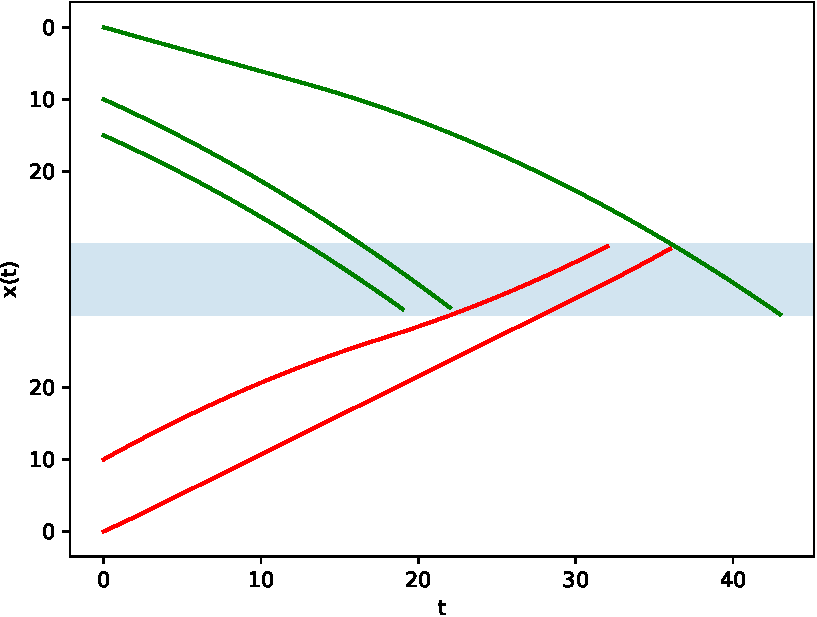
\includegraphics[width=0.9\textwidth]{figures/single/trajectories_general.pdf}%
  \end{minipage}
  \begin{minipage}{0.23\textwidth}
  \vspace*{-1em}
  \begin{tabular}{ c c c }
    $i$ & $x_{i}^{0}$ & $v_{i}^{0}$ \\[0.2em]
    \hline\\[-1em]
    {\color{red}(1,3)} &  0 & 1.0 \\
    {\color{red}(1,2)} & 10 & 1.0 \\
    {\color{red}(1,1)} & 15 & 1.0 \\
    {\color{blue}(2,1)} & 10 & 0.8 \\
    {\color{blue}(2,2)} &  0 & 0.0
  \end{tabular}
  \\[2em]
  \begin{tabular}{ c c c }
    $L$ & = &  5 \\
    $\mathcal{E}$ & = & $[20, 30]$ \\
    $\bar{v}$ & = & 1 \\
    $\omega, \bar{\omega}$ & = & 0.1 \\
    $K$ & = & 50 \\
    $\Delta t$ & = & 1
  \end{tabular}
  \end{minipage}
  \caption{Example of optimal trajectories minimizing $J_{\alpha,\beta}$ (solid)
    and $J_{v_{d}}$ (dashed), obtained using the direct transcription method for
    cost parameters $\alpha = -1, \, \beta = 100$ and $v_{d} = 0.6$. The system
    parameters and initial conditions are listed next to the figure. The y-axis
    is split such that the top part corresponds to route $1$ and the bottom to
    route $2$ and the trajectories are inverted accordingly and drawn with
    separate colors. The interval of intersection-occupying positions
    $\mathcal{E}$ is drawn as a shaded region. Trajectories
    are not drawn beyond this region.}%
  \label{fig:direct_transcription_example}
\end{figure}

\section{Occupancy time slots and trajectories}\label{sec:decomposition}

% The main goal of this section is to explain how the trajectory optimization
% problem~\eqref{eq:T} can be reduced to a scheduling
% problem.
% %
% First, we show how to rewrite~\eqref{eq:T} in terms of two coupled optimization
% problems: an upper-level scheduling problem, dictating the occupancy time slots,
% and a lower-level trajectory optimization problem for each group of vehicles on
% the same route. We explain how this reformulation has been used as the basis for
% an approximation algorithm in~\Cref{sec:approx-algos}.
% %
% We close this chapter by showing in~\Cref{sec:delay-minimization} that the
% decomposition becomes \emph{proper} when the optimization objective only involves
% delay, and we assume that vehicles enter the intersection at full speed. This
% means that the upper-level problem can first be solved separately to obtain an
% optimal time schedule, after which the lower-level problems can be resolved, for
% each route separately. This proper decomposition reformulation is the starting
% point of the remaining chapters.
 
Given some feasible trajectory $x_{i} \in D(s_{i})$ for a single vehicle $i$, we
define its (earliest) \emph{crossing} time and (earliest) \emph{exit} time,
respectively, to be
%
\begin{subequations}
\begin{alignat}{2}
  \tau(x_{i}) &:=& \, \min &\{ t \in [0, t_{f}] : x_{i}(t) = B \} , \\
  \xi(x_{i}) &:=& \, \min &\{ t \in [0, t_{f}] : x_{i}(t) = E + L \} .
\end{alignat}
\end{subequations}
%
Observe that $\tau(x_{i})$ and $\xi(x_{i})$ specify the times
$t \in (\tau(x_{i}), \xi(x_{i}))$ when vehicle $i$ occupies the
intersection\footnote{%
  Note that the sets in the definition are closed, because $x_{i}$ is continuous
  by assumption, but they may be empty. Therefore, we use the convention that
  ``$\min \varnothing = \infty$'', such that $\tau(x_{i}) = \infty$ whenever
  $x_{i}$ does not reach the intersection at all and, analogously, we have
  $\xi(x_{i}) = \infty$ whenever the end of the intersection is never reached.
  Furthermore, we use the convention that
  ``$(\infty, \infty) = \varnothing$''.}. Hence, we will refer to
$(\tau(x_i), \xi(x_i))$ as the \emph{occupancy time slot} of vehicle $i$.

Recall the encoding of the collision constraints using binary variables
in~\eqref{eq:collision-avoidance-binary-encoding}.
%
Similarly, observe that the collision-avoidance constraints
\begin{align*}
  (x_{i}(t), x_{j}(t)) \notin \mathcal{E}^{2} \quad \text{ for all } \{i,j\} \in \mathcal{D}
\end{align*}
are completely equivalent to the constraints
\begin{align}\label{eq:disjoint-occupancy}
  \big(\tau(x_{i}), \xi(x_{i}) \big) \cap \big(\tau(x_{j}), \xi(x_{j})\big) = \varnothing \quad \text{ for all } \{i,j\} \in \mathcal{D} .
\end{align}

\subsection{Bilevel decomposition}\label{sec:bilevel}
The main idea of the decomposition is to make these crossing and exit times
concrete decision variables of the upper-level problem.
%
Hence, for each vehicle $i$, we introduce a decision variable $y_{i}$ for the
time of crossing and a variable $z_{i}$ for the time of exit.
%
When the occupancy time slots $\{(y_{i}, z_{i}) : i \in \mathcal{N}\}$ are fixed
and satisfy~\eqref{eq:disjoint-occupancy}, the trajectory optimization problem
essentially reduces to solving a separate lower-level problem for each route.

Before we make this precise, let us first introduce some notation for
collections of parameters and variables pertaining to a single route.
%
Recall that $\mathcal{N}_{r}$ denotes all vehicles on route $r$.
We write $s_{r} := \{(x_{i}^{0}, v_{i}^{0}) : i \in \mathcal{N}_{r} \}$ to
denote the corresponding initial conditions and we write
$x_{r} := \{x_{i} : i \in \mathcal{N}_{r} \}$ as a shorthand for a set of
trajectories on route $r$.

\paragraph{Lower-level problem.}
Consider some route $r \in \mathcal{R}$ with local initial conditions $s_{r}$ and
suppose we are given some fixed local occupancy time slots as determined by
$y_{r} := \{y_{i} : i \in \mathcal{N}_{r}\}$ and
$z_{r} := \{z_{i} : i \in \mathcal{N}_{r}\}$, then we define the lower-level
\emph{control problem}
%
\begin{alignat}{3}\label{eq:lower-level}
  F(y_{r},z_{r}, s_{r}) := \min_{x_{r}} \;\, & \sum_{i \in \mathcal{N}_{r}} J(x_{i}) \tag{L} \\
  \text{s.t. } \; & x_{i} \in D(s_{i})  && \quad \text{ for all } i \in \mathcal{N}_{r} , \tag{L.1} \label{eq:L1} \\
  & x_{i}(t) - x_{j}(t) \geq L && \quad \text{ for all } (i,j) \in \mathcal{C} \cap \mathcal{N}_{r}^2 , \tag{L.2} \label{eq:L2} \\
  & x_{i}(y_i) = B  && \quad \text{ for all } i \in \mathcal{N}_{r} , \tag{L.3} \label{eq:L3} \\
  & x_{i}(z_{i}) = E + L  && \quad \text{ for all } i \in \mathcal{N}_{r} . \tag{L.4} \label{eq:L4}
\end{alignat}
%
Note that the feasibility of this problem depends on the initial states as well
as the choice of occupancy time slots. Therefore, given initial states $s_{r}$,
we write $(y_{r}, z_{r}) \in \mathcal{S}(s_{r})$ to denote the set of occupancy
time slots for which~\eqref{eq:lower-level} is feasible, which we call
\emph{feasible route schedules}.

\paragraph{Upper-level problem.}
The upper-level problem is now to find a set of occupancy time slots
satisfying~\eqref{eq:disjoint-occupancy}, such that the lower-level problem for each route is feasible.
Let $s = \{s_{r} : r \in \mathcal{R} \}$ denote the set of global initial states for
all routes and write $y = \{y_{r} : r \in \mathcal{R} \}$ and
$z = \{y_{z} : r \in \mathcal{R}\}$ to denote a set of global occupancy time slots,
then we define the upper-level \emph{scheduling problem}
%
\begin{alignat}{2}\label{eq:upper-level}
  U(s) := \min_{y, z} \quad & \sum_{r \in \mathcal{R}} F({y}_{r}, {z}_{r}, s_{r}) \tag{U} \\
  \text{ s.t. } \quad & (y_{i},z_{i}) \cap (y_{j},z_{j}) = \varnothing & \quad \text{ for all } \{i, j\} \in \mathcal{D} , \tag{U.1} \label{eq:U1} \\
                            & ({y}_{r}, {z}_{r}) \in \mathcal{S}(s_{r}) & \text{ for all } r \in \mathcal{R} . \tag{U.2}
\end{alignat}

\paragraph{Forced crossing.}
Without further assumptions, problem~\eqref{eq:upper-level} is almost equivalent to the original problem~\eqref{eq:T}.
%
As we already noted when defining cost functionals, there is a subtle issue in the fact
that a feasible solution $x$ of~\eqref{eq:T} does not necessarily cross the intersection.
%
To avoid this, we explicitly require the crossing and exit times to be finite,
which yields variant~\eqref{eq:T*}. With this technical assumption, we briefly
sketch how validity of the decomposition can be established rigorously.
\begin{alignat}{3}\label{eq:T*}
  T'(s) := \min_{x} \;\, & \sum_{i \in \mathcal{N}} J(x_{i}) \tag{$\mathrm{T}'$} \\
  \text{s.t. } \; & x_{i} \in D(s_{i}) && \quad \text{ for all } i \in \mathcal{N} , \tag{T.1} \\
           & x_{i}(t) - x_{j}(t) \geq L && \quad \text{ for all } (i,j) \in \mathcal{C} , \tag{T.2} \\
           & (x_{i}(t), x_{j}(t)) \notin \mathcal{E}^{2} && \quad\text{ for all } \{i, j\} \in \mathcal{D} , \tag{T.3} \label{eq:T*.3} \\
           & \tau(x_{i}) < \infty && \quad \text{ for all } i \in \mathcal{N} , \tag{$\mathrm{T}'.4$} \label{eq:T4*} \\
           & \xi(x_{i}) < \infty && \quad  \text{ for all } i \in \mathcal{N} . \tag{$\mathrm{T}'.5$} \label{eq:T5*}
\end{alignat}

\begin{theorem}[{\cite[Theorem 1]{hultTechnicalReportApproximate}}]\label{thm:decomposition}
  Assume problem~\eqref{eq:T*} is feasible and an optimal solution exists, then it is
  equivalent to the decomposed problem~\eqref{eq:upper-level}.
\end{theorem}
\begin{proof}[Proof (sketch).]
  Given some initial state $s$, let $\mathcal{X}(s)$ denote the feasible
  trajectories of~\eqref{eq:T*} and let $\mathcal{S}(s)$ denote the feasible
  schedules of~\eqref{eq:upper-level}. We argue that each
  $(y,z) \in \mathcal{S}(s)$ can be transformed into a feasible solution
  $x \in \mathcal{X}$ and vice versa.

  Let $(y^*,z^*)$ be a feasible solution of~\eqref{eq:upper-level} and let $x^*$ denote some
  corresponding set of trajectories obtained by solving~\eqref{eq:lower-level}, which are not
  necessarily unique. Since $x^*$ satisfies $x^*_{i}(y^*_{i}) = B$ and
  $x^*_{i}(z^*_{i}) = E + L$, we see that $\tau(x^*_{i}) < \infty$ and $\xi(x^*_{i}) < \infty$.
  Because~\eqref{eq:L3} and~\eqref{eq:L4} are together equivalent to~\eqref{eq:T*.3}, we see that $x^*$ is also
  a feasible solution to~\eqref{eq:T*}. Hence,
  %
  \begin{align}\label{eq:U-T}
    \sum_{r \in \mathcal{R}} F(y^*_r, z^*_r, s_r) = \sum_{i \in \mathcal{N}} J(x^*_i) \geq T'(s) .
  \end{align}
  %
  Conversely, let $x'$ be some solution to~\eqref{eq:T*}, then $y'_{i} := \tau(x_{i})$ and
  $z'_{i} := \xi(x_{i})$ for all $i$ are \emph{uniquely defined}. Because $x'$
  satisfies~\eqref{eq:T*.3}, we are sure that $y'$ and $z'$ satisfy~\eqref{eq:U1} and $x'_{r}$ are
  obviously feasible for the lower-level problems. Hence,
  %
  \begin{align}\label{eq:T-U}
    \sum_{i \in \mathcal{N}} J(x'_i) = \sum_{r \in \mathcal{R}} \sum_{i \in \mathcal{N}_r} J(x'_i)
    \geq \sum_{r \in \mathcal{R}} F(y'_r, z'_r, s_r)
    \geq U(s) .
  \end{align}
  % 
  Finally, taking $\min_{y^*,z^*}$ in~\eqref{eq:U-T} and $\min_{x'}$ in~\eqref{eq:T-U}
  yields $U(s) = T'(s)$, as desired.
\end{proof}


\subsection{Decomposition-based approximation algorithms}\label{sec:approx-algos}

Even with this decomposition, the problem is still difficult to solve.
%
In general, the difficulty of solving~\eqref{eq:upper-level} lies in the fact that $F$ is a
non-trivial function of the occupancy time slots and $\mathcal{S}(s_{r})$ is not
easily characterizable, e.g., as a system of inequalities. In other words, we
could say that the upper- and lower-problem are \emph{tightly coupled} by
feasibility.

Nevertheless, the decomposition provides a good conceptual basis for
approximation algorithms.
%
One approach that has been explored in the literature is to explicitly
approximate the set of feasible time slots $\mathcal{S}(s_r)$ and the objective
function $F$.
%
Suppose we have a single vehicle per route, so $n_r = 1$ for all
$r \in \mathcal{R}$ and $(y_{r}, z_{r}) \equiv (y_{i},z_{i})$.
%
For this case, the following approximation scheme has been proposed~\cite{hultApproximateSolutionOptimal2015}. 

Evaluate $F(y_{i}, z_{i}, s_{i})$ at fixed grid points to fit a strictly convex approximation $\hat{F}$.
%
Next, the set of feasible occupancy slots can be estimated by the following
polyhedral subset
\begin{align}
  \hat{\mathcal{S}}(s_i) = \{ (y, z) : y \in [T_{i}^{l},T_{i}^{h}], \; l_{i}(y) \leq z \leq u_{i}(y) \} \subseteq \mathcal{S}(s_{i}) .
\end{align}
Here, the occupancy time slot is required to be between the earliest crossing time
$T_{i}^{l}$ and the latest crossing time $T_{i}^{h}$. Roughly speaking, these
bounds can simply be computed by finding the fastest and the slowest route,
respectively.
%
The exit time bounds $u_{i}(y)$ and $l_{i}(y)$ are strictly increasing affine.

The approximations $\hat{F}$ and $\hat{\mathcal{S}}$ turn the upper-level problem into a
mixed-integer quadratic problem, which has been shown to be easier to solve than
the original direct transcription, but at the cost of suboptimality. Of course,
the set $\mathcal{S}(s_i)$ is larger than its polyhedral approximation, so
optimality is not guaranteed.
%
The authors prove~\cite{hultTechnicalReportApproximate} that this
scheme does not affect feasibility of the problem.


\subsection{Isolating the timing problem}\label{sec:delay-minimization}

Although the approximation approach sketched above is very interesting, we will
not aim to tackle the problem in its full generality, by making some mild
assumptions that expose and separate the combinatorial nature of the problem.

\begin{assump}[Full speed]
  We assume that all vehicles in the system start at full speed
  $v_{i}^{0} = \bar{v}$ and enter the intersection at full speed.
  Therefore, we add $\dot{x}_{i}(\tau(x_{i})) = \bar{v}$ as additional constraint
  to~\eqref{eq:T*} and, equivalently, we add $\dot{x}_{i}(y_{i}) = \bar{v}$ to the
  lower-level problem~\eqref{eq:lower-level}.
\end{assump}

\begin{define}[Earliest crossing time]
  Given some trajectory $x_i$ with initial state $s_i = (x_i^0, \bar{v})$, define
  the \emph{earliest crossing time} of vehicle $i$ to be
  \begin{align}
    \label{eq:5}
    a_i := (B - x_i^0) / \bar{v} .
  \end{align}
\end{define}

\begin{define}
  Suppose some vehicle drives at full speed as long as it occupies the
  intersection. In that case, the vehicle occupies the intersection for a duration of precisely
  \begin{align}
    \sigma := (E+L-B)/\bar{v} .
  \end{align}
  %
  Furthermore, define the \emph{processing time}
  \begin{align}
    \rho := L / \bar{v} .
  \end{align}
  %
  We will call the difference $\delta := \sigma - \rho$ the \emph{switch-over
    time}, which is non-negative by definition.
\end{define}

\begin{define}[Delay criterion]
  We introduce the following simple trajectory cost criterion. Let the \emph{delay criterion}
  be defined $J_d(x_i) = \tau(x_i) - a_i$. To simplify notation in the
  next chapter, we will also consider the related criterion
  $J'_d(x_i) = \tau(x_i)$.
\end{define}

The delay criterion simplifies our problem significantly, because $F$ becomes a
trivial function of the start times of the occupancy time slots. For every route
$r \in \mathcal{R}$, we have
\[
\renewcommand{\arraystretch}{1.2}
\begin{NiceArray}{ r @{\;} l l l }
  F(y_r, z_r, s_r) &= \displaystyle \min_{x_r}   \sum_{i \in \mathcal{N}_r} J_d(x_i) & \quad \text{ s.t. } \mathrm{(\ref{eq:L1},\ref{eq:L2},\ref{eq:L3},\ref{eq:L4})} \\[20pt]
  &= \displaystyle \min_{x_r} \sum_{i \in \mathcal{N}_r} \tau(x_i) - a_i & \quad \text{ s.t. } \mathrm{(\ref{eq:L1},\ref{eq:L2},\ref{eq:L4})} & \\[-12.5pt]
  &&& \hspace{0.2em} = \displaystyle \sum_{i \in \mathcal{N}_r} y_i - a_i , \\[-10pt]
  & \quad\quad\quad \text{ s.t. } x_i(y_i) = B & \quad \text{ for all } i \in \mathcal{N}_r
  \CodeAfter\SubMatrix.{2-2}{4-3}\}
\end{NiceArray}
\]
%
such that the upper-level problem reduces to
%
\begin{subequations}\label{eq:C-pre}
\begin{alignat}{2}
  U(s) = \min_{y, z} \quad & \sum_{i \in \mathcal{N}} y_{i} - a_i \\
  \text{ s.t. } \quad & (y_{i},z_{i}) \cap (y_{j},z_{j}) = \varnothing && \quad \text{ for all } \{i, j\} \in \mathcal{D} ,  \\
                           & ({y}_{r}, {z}_{r}) \in \mathcal{S}(s_{r}) && \quad \text{ for all } r \in \mathcal{R} .
\end{alignat}
\end{subequations}

% \paragraph{Feasibility characterization.}
%

The difficulty that remains is how to pick occupancy schedules that guarantee
feasibility of the lower-level problem.
%
Given some $(y,z) \in \mathcal{S}(s)$, every lower-level solution $x_{i}$
satisfies $\dot{x}_{i}(y_{i}) = \bar{v}$, so we can safely let vehicles continue
at full speed across the intersection, because $z_{i}$ is not involved in
$J_d(\cdot)$.
%
In that case, each vehicle leaves the intersection completely after
$\sigma$ time, so we fix
\begin{align*}
  z_{i} = y_{i} + \sigma, \; \text{ for all } i \in \mathcal{N} .
\end{align*}
%
Observe that $\sigma$ is the minimum time between the crossing times of
vehicles from conflicting routes.
%
Consequently, we can limit ourselves to
\begin{align}
  \label{eq:1}
  \mathcal{Y}(s_{r}) := \{ y_{r} : (y_{r}, y_{r} + \sigma) \in \mathcal{S}(s_{r}) \} ,
\end{align}
where $y_{r} + \sigma$ means $\{y_{i} + \sigma : i \in \mathcal{N}_{r}\}$.
%
Similarly, $\rho$ is the minimum time between crossing times of vehicles on the
same route.
% 
The sufficient conditions of Assumption~\ref{assump:feasible} allow a polyhedral characterization
of $\mathcal{Y}(s_r)$; it can be shown\footnote{A rigorous proof of this fact is
  outside the scope of the current project.} that
%
\begin{align}\label{eq:feasibility-inequalities}
 y_{r} \in \mathcal{Y}(s_{r}) \iff
 \begin{cases}
  a_{i} \leq y_i & \; \text{ for all } i \in \mathcal{N}_{r} , \\
  y_i + \rho \leq y_j & \; \text{ for all } (i,j) \in \mathcal{C} \cap \mathcal{N}^2_{r} .
  \end{cases}
\end{align}
%
Hence, problem~\eqref{eq:C-pre} reduces to the following \textit{crossing time scheduling} problem:

\begin{mdframed}
\vspace{-\abovedisplayskip}
\begin{alignat}{2}\label{eq:C}
  \min_{y} \quad & \sum_{i \in \mathcal{N}} y_i - a_i \tag{C} \\
  \text{ s.t. } \quad & a_{i} \leq y_i  && \quad \text{ for all } i \in \mathcal{N} , \tag{C.1} \\
                    & y_i + \rho \leq y_{j}  && \quad \text{ for all } (i,j) \in \mathcal{C} \label{eq:conjunctive} , \tag{C.2} \\
                    & (y_{i}, y_i + \sigma) \cap (y_{j}, y_j + \sigma) = \varnothing && \quad \text{ for all } \{i,j\} \in \mathcal{D} \label{eq:disjunctive} \tag{C.3}.
\end{alignat}
\end{mdframed}

This is a typical scheduling problem, which can, for example, be solved within
the mixed-integer linear programming framework after encoding the \textit{disjunctive
  constraints}~\eqref{eq:disjunctive} using the big-$M$ technique, which we will do in
the next chapter.


\paragraph{Instances and schedules.}

The next chapter will be about solving~\eqref{eq:C}, so let us first take a step back and
spend a few words on explaining our notation for specifying (sets of) instances
of this problem.
%
We will write $a := \{ a_i \}_{i \in \mathcal{N} }$ to denote the set of
\emph{earliest crossing times}.
%
We will mostly keep the indices $\mathcal{N}$ implicit in this notation; when
necessary, we write $\mathcal{N}(a)$.
%
Note that $R$, $\{n_r\}_{r \in \mathcal{R}}$, $\mathcal{C}$ and $\mathcal{D}$
are all uniquely determined by $\mathcal{N}(a)$; we use similar notation when we
need to stress that they belong to $a$.
%
Therefore, we will write an instance of~\eqref{eq:C} as a triple
%
\begin{align*}
  (a, \rho, \sigma) .
\end{align*}

It follows immediately from its definition that $a$ has to satisfy the following
property, which is stated here for easy reference.

\begin{proposition}\label{lemma:arrivals}
  The arrival times satisfy $a_i + \rho \leq a_j$, for each conjunctive pair $(i, j) \in \mathcal{C}$.
\end{proposition}

% sets of instances
% In order to analyze the performance of solution methods for~\eqref{eq:C}, we will
% define a set of instances $\mathcal{I}$.
% %
% To keep the analysis simple, we will assume that the number of route $R$ and the
% times $\rho$ and $\sigma$ are fixed and equal among all instances in $\mathcal{I}$.
% %
% Later, we will induce a probability distribution over $\mathcal{I}$ to model the
% relative importance or occurence of particular problem instances in practical
% contexts.

Throughout the rest of this thesis, we will use a simple way of visualizing
problem instances and candidate solutions that is somewhat similar to the
classical Gantt chart: we use a bar chart with time on the vertical axis.
%
Each row corresponds to one of the routes of the instance and each vehicle
is represented by a block, whose width corresponds to the fixed processing
time $\rho$.
%
The block for vehicle $i$ is positioned such that its 
left border is located at the earliest crossing time $a_i$.
%
For example, Figure~\ref{fig:instance-example} depicts some instance with
\begin{align*}
  a = \{&a_{11} = 0.31, \; a_{12} = 1.78, \\
        &a_{21} = 0.74, \; a_{22} = 2.86, \; a_{23} = 4.60 \} .
\end{align*}

To visualize some candidate schedule $y$, we collapse all the route rows into a
single row, see Figure~\ref{fig:solution-example}, such that every block starts at the schedule time
$y_i$. Therefore, every block represents the crossing time slot that is
allocated to the corresponding vehicle. We sometimes add arrows of length
$\delta = \sigma - \rho$ to illustrate the necessary switch-over time between
consecutive time slots for different routes.

\def\vizfigscale{0.90}
\begin{figure}[h]
  \centering
  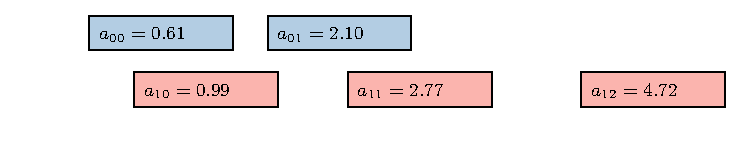
\includegraphics[scale=\vizfigscale]{../single/figures/instance}
  \caption{Instance example with earliest arrival times indicated for each vehicle.}%
  \label{fig:instance-example}
\end{figure}

\begin{figure}[h]
  \centering
  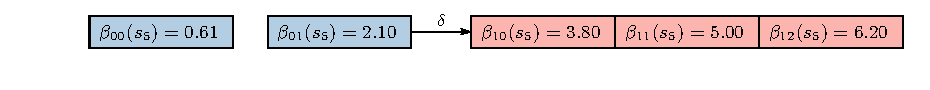
\includegraphics[scale=\vizfigscale]{figures/single/schedule}
  \caption{Some schedule as example solution to the problem instance shown in Figure~\ref{fig:instance-example}.}%
  \label{fig:solution-example}
\end{figure}

\pagebreak
\section{Notes and references}

The single intersection model is mostly based on the model described in the PhD
thesis of Hult~\cite[Chapter 3]{hultOptimizationBasedCoordination2019}.
%
Due to the simple rectangular geometry of the vehicles and the fact that routes
are straight, it is easy to compute the conflict area in configuration space,
for which we provide details in Appendix~\ref{app:configuration-space}. For
general curved trajectories, the computation is more involved, see for
example~\cite[Appendix A]{levinConflictpointFormulationIntersection2017}
and~\cite[Section 2.2]{liTemporalspatialDimensionExtensionbased2019}.

The bilevel decomposition and approximation scheme of Section~\ref{sec:bilevel}
are further detailed in~\cite{hultApproximateSolutionOptimal2015,hultTechnicalReportApproximate}.
%
In proving that the decomposed problem is equivalent to the original trajectory
optimization problem, they state that the lower-level problem has a unique
solution. We emphasize that this depends on \emph{strict} convexity of the objective function.
%
For the problem without state constraints, this has been rigorously proven in~\cite[Theorem 5.1, part
(V)]{hanUnifiedNumericalScheme2012}, where uniqueness indeed depends on the positive
definiteness of the matrix $R$ defining the quadratic component $u^T R u$ of the
running cost function with respect to the control variable.

At the end of this section, we included some comments from the optimal control
perspective. For a textbook introduction of optimal control theory, we recommend
the book of Liberzon~\cite{liberzonCalculusVariationsOptimal}. The focal point
in their presentation is the Pontryagin maximum principle, which provides
neccessary conditions for optimality for optimal control problems.
%
When dealing with state-constrained problems, the most relevant overview of
results we could find is the survey of Hartl et
al.~\cite{hartlSurveyMaximumPrinciples1995}.
%
We note that, although the theory for dealing with state constraints (\`a la
Pontryagin) is far from complete, in practice, they can be successfully dealt
with in numerical approaches, often involving some sort of penalty function.

% \begin{remarknum}\label{rem:state-constraints}
%   Infinite-dimensional optimization problems like~\eqref{eq:T} are typically
%   studied in the framework of optimal control theory.
%   %
%   In this context, the joint position $x = \{x_{i} : i \in \mathcal{N}\}$ is
%   referred to as the \emph{state} of the system and
%   $\ddot{x} = \{\ddot{x}_{i} : i \in \mathcal{N} \}$ as the \emph{control}.
%   %
%   Acceleration is understood to be the main input of the system, such that the
%   joint vehicle position is indirectly determined by integrating twice. For this
%   reason, this simple vehicle dynamics model is commonly referred to as the \emph{double
%     integrator}.
%   %
%   The canonical optimal control problem is defined in terms of finding some
%   continuous function $x(t) \in \mathbb{R}^{n}$ and some integrable function
%   $u(t) \in \mathbb{R}^{m}$, satisfying the equations
%   \begin{align}\label{eq:general-dynamics}
%     \dot{x} = f(t, x, u) , \quad x(t_{0}) = x_{0} , \quad u \in U \subset \mathbb{R}^{m},
%   \end{align}
%   given some initial state $x_{0}$ and initial time $t_{0}$ and some (compact)
%   control set $U$. Given some final time $t_{f}$, a running cost function
%   $\mathcal{L}$ and some terminal cost function $\mathcal{K}$, the goal is to
%   \begin{subequations}\label{eq:opt-control}
%   \begin{align}
%     \min_{x} \; & \int_{t_{0}}^{t_{f}} \mathcal{L}(t, x(t), u(t)) \diff t + \mathcal{K}(t_{f}, x_{f}) , \\
%       \textnormal{such that } \, &\eqref{eq:general-dynamics} \textnormal{ holds, } \\
%                     & h(x) = 0 , \label{eq:state-constr-eq} \\
%                     & g(x) \leq 0 , \label{eq:state-constr-ineq}
%   \end{align}
%   \end{subequations}
%   with some functions $h : \mathbb{R}^{n} \rightarrow \mathbb{R}^{p}$ and
%   $g : \mathbb{R}^{n} \rightarrow \mathbb{R}^{q}$ encoding the so-called state
%   constraints. Functions $f, g, h$ are usually assumed to possess certain
%   regularity or smoothness properties.
%   %
%   There are general methods to analyze optimal solutions
%   of~\eqref{eq:opt-control}, most notably the necessary conditions given by the
%   maximum principle of Pontryagin~\cite{liberzonCalculusVariationsOptimal}.
%   %
%   However, the occurrence of state constraints like~\eqref{eq:state-constr-eq}
%   and~\eqref{eq:state-constr-ineq} make such analysis notoriously difficult and
%   remains an area of ongoing research~\cite{hartlSurveyMaximumPrinciples1995}.
%   %
%   For our current problem, note that the collision-avoidance constraints~\eqref{eq:T2}
%   and~\eqref{eq:T3}, as well as the speed constraint~\eqref{eq:speed-constr} contained in~\eqref{eq:T1}, are all of the
%   type~\eqref{eq:state-constr-ineq}.
% \end{remarknum}


\chapter{Crossing time scheduling}\label{chap:crossing-time-scheduling}

Problems like~\eqref{eq:C} have been studied extensively, so we first discuss
traditional solution methods.
%
Our problem is a combinatorial optimization problem, for which a wealth of
general solution techniques is
available~\cite{duIntroductionCombinatorialOptimization2022}, including
algorithms specifically tailored to the case when feasible solutions can be
thought of as time
schedules~\cite{pinedoSchedulingTheoryAlgorithms2016,grahamOptimizationApproximationDeterministic1979}.
%
One of the most prominent distinction among algorithms lies in whether it
guarantees to find an optimal solution or not.
%
Of course, it is desirable to find optimal solutions, but this is often not
tractable in practice: the number of feasible solutions typically explodes
whenever larger instances are considered---it is virtually impossible to
enumerate all feasible solutions, evaluate their objective value, and pick the
best one, in any reasonable amount of time.

\paragraph{Integer programming.}
The first part of this chapter illustrates a standard method of dealing with
combinatorial problems, in which the discrete decision are encoded as integers.
More specifically, in~\Cref{sec:branch-and-bound}, we show how~\eqref{eq:C} can
be formulated as a \emph{mixed-integer linear
  programming}~\cite{confortiIntegerProgramming2014}, which can be solved in a
principled way using the branch-and-bound strategy. Integer programming is a
mature technology, as reflected in the availability of general solvers and
software tooling.
%
By leveraging insight into the structure of optimal solutions, we are able to
formulate three problem-specific cutting planes, yielding an efficient
algorithm for coordination at a single intersection.
%
We conclude the first part of this chapter by evaluating how much the running
time is reduced by these cutting planes.

\paragraph{Constructive heuristics.}
In many practical applications---like in our case of motion planning for
autonomous vehicles---the time that is available to obtain a solution is
limited. Hence, it is not essential to obtain the best solution. This is the
main motivation for the development of so-called heuristics, which discard the
optimality guarantee in favor of speed. In other words, we want a good solution,
fast!

While integer programming can be interpreted as a smart exhaustive search over
the space of feasible solutions, we will consider a simple class of heuristic
algorithms that is based on a simple step-by-step construction.
%
\Cref{sec:sequence-representation} provides the necessary setup required for our
methodology.
%
Specifically, we use a simple graph reformulation of~\eqref{eq:C} to show that
it can be reduced to a problem of finding a sequence of route indices, which we
will call the \emph{route order}. The resulting route order is the starting
point for our discussion in~\Cref{chap:single-learning}, where we propose to use
techniques from machine learning to automate the process of developing an
algorithm for finding good route orders.


\section{Integer programming}\label{sec:branch-and-bound}

% - first explain the general algorithmic branch-and-bound paradigm
% - then provide a brief general intro of MILP, pointing out its strengths and weaknesses

One of the fundamental algorithmic ideas in combinatorial optimization is the
branch-and-bound strategy, in which the space of feasible solutions is
systematically explored by keeping track of the search tree and iteratively
subdividing the feasible region into smaller subproblems (branching), computing
bounds on the best possible objective value within each subproblem (bounding),
and discarding those parts of the feasible region that contain subproblems whose
bound proves them incapable of containing an optimal solution (pruning).

The branch-and-bound scheme is found in algorithms for solving mixed-integer
programming problems.
%
In such problems, we optimize over $n$ real-valued decision variables $y_{i}$
for which possibly a subset $\mathcal{I} \subseteq \{1, \dots, n\}$ is
restricted to be integer-valued.
%
A canonical example of such problems is the mixed-integer linear program, where
the goal is to minimize
\begin{align}\label{eq:MILP}\tag{MILP}
  \min_{y} c^{T} y \text{ such that } Ay \leq b, \; y \in \mathbb{R}^{n}, \; y_{j} \in \mathbb{Z} \text{ for } j \in \mathcal{I},
\end{align}
given some matrix $A \in \mathbb{R}^{m\times n}$ and vectors
$b \in \mathbb{R}^{m}$ and $c \in \mathbb{R}^{n}$.
%
This surprisingly simple setup provides a powerful modeling toolkit to approach
many combinatorial optimization problems, because it allows discrete choices to
be modeled using integers.
%
We already saw an example of this when we applied the big-$M$ method in our
direct transcription of the trajectory optimization problem.

The branch-and-bound algorithm for~\eqref{eq:MILP} is based on progressively
constraining the integer decision variables as we move further from the root
node in the search tree.
%
At each node, the integer constraints are relaxed, producing a linear program
that can be solved efficiently.
%
The solutions of these relaxations provide the basis of the bounding step:
whenever the objective of the relaxation at some node is higher than that of the
currently best known feasible solution, the subtree at that node is pruned.

\subsection{Reformulation as MILP}

We show how to reformulate the crossing time scheduling
problem~\eqref{eq:C} into the form~\eqref{eq:MILP}. Note that we
only have to rewrite the disjunctive constraints~\eqref{eq:disjunctive}. For
each conflict $\{i,j\} \in \mathcal{D}$, this constraints essentially encodes
the crossing order of $i$ and $j$, i.e., whether $i$ crosses the intersection
before $j$, or vice versa.
%
We can rewrite these constraints using the big-$M$ method by introducing a
binary decision variable $\gamma_{ij}$ for every conflict $\{i, j\} \in \mathcal{D}$,
such that setting $\gamma_{ij} = 0$ corresponds to choosing the crossing order
$i \rightarrow j$ and $\gamma_{ij} = 1$ corresponds to $j \rightarrow i$.
%
To avoid redundant variables in a software implementation, it might be desirable
to induce some arbitrary ordering of the conflicting vehicles by defining the
index set
\begin{align}
  \bar{\mathcal{D}} = \{ (i,j) : \{i,j\} \in \mathcal{D}, \; r(i) < r(j) \} .
\end{align}
With this definition, we obtain the MILP reformulation
%
\begin{equation}\tag{$\mathrm{C}^\prime$}\label{eq:C'}
\renewcommand{\arraystretch}{1.2}
\begin{NiceArray}{ r l @{} >{{}}c<{{}} @{} l @{} }
  \displaystyle \min_{y,\gamma} & \displaystyle \sum_{i \in \mathcal{N}} y_{i} \\
  \text{s.t. } \; & a_{i} \leq y_{i} && \quad \text{ for all } i \in \mathcal{N} , \\
  & y_{i} + \rho \leq y_{j} && \quad \text{ for all } (i,j) \in \mathcal{C} , \\
  & y_{i} + \sigma \leq y_{j} + \gamma_{ij}M  &&  \\
  & y_{j} + \sigma \leq y_{i} + (1 - \gamma_{ij})M \hspace*{1.8em} && \quad \text{ for all } (i,j) \in \bar{\mathcal{D}} , \\
  & \gamma_{ij} \in \{0, 1\}
\CodeAfter\SubMatrix.{4-1}{6-2}\}
\end{NiceArray}
\end{equation}
%
where $M > 0$ is some sufficiently large number.

\begin{remarknum}\label{rem:delay-objective}
  The careful reader may observe that we removed the earliest arrival times
  $a_i$ from the delay criterion. Since $a$ is assumed to be given, we can
  always compute the original delay cost by subtracting $\sum_i a_i$.
\end{remarknum}

Note that this reformulating opens up the possibility to leverage the collective
effort that has gone into developing fast general solvers for this problem
class: many modern solvers, e.g., SCIP~\cite{BolusaniEtal2024OO} (academic) or
Gurobi~\cite{gurobi} (commercial), employ specialized interal heuristics and
techniques to derive better bounds and thus achieve more pruning of the search
tree to speed up the solving process.
%
Furthermore, a wide variety of software tooling is available. For example, we
used the AMPL modeling language to write the above formulation in a
solver-agnostic specification and use the
amplpy\footnote{\url{https://amplpy.ampl.com/}} package to call the solver from
the comfort of Python.
%
We report some numerical results based on this method in
\Cref{sec:runtime-bench}. First, we show that the above formulation can be made
a little sharper.


\subsection{Optimal substructure: platoons}\label{sec:platoons}

The branch-and-bound approach guarantees to find an optimal solution, but it
does not provide any guarantees on the required running time.
%
Roughly speaking, the running time depends mainly on two aspects: (i) size of
the instance---in our case: number of vehicles---and (ii) the amount of structure it
exhibits.
%
More specifically, the running time depends heavily on the efficiency of the
bounding step in pruning the search tree, which might vary wildly among
equivalent formulations.
%
A technique that is often used to make bounding more efficient is to add
so-called \emph{cutting planes}.
%
The basic idea is that we can introduce additional inequalities
without changing the set of feasible solutions
\begin{align}
  \{ y : Ay \leq b, A'y \leq b', y_j \in \mathbb{Z}, j \in \mathcal{I} \} = \{ y : Ay \leq b, y_j \in \mathbb{Z}, j \in \mathcal{I} \} ,
\end{align}
while achieving more efficient bounding.
%
There are general-purpose schemes for adding such cutting planes $A' y \leq b$,
but it often makes sense to also use insights into the specific problem at hand
to derive problem-specific cutting planes.
%
The branch-and-bound framework with cutting planes is colloqially referred to as
\emph{branch-and-cut}.

Next, we present insight into some optimal substructures of optimal solutions.
This analysis will serve as the basis for defining three types of cutting
planes.
%
Let us first consider some simple problem instances to start shaping our
intuition.

\begin{figure}[t]
  \centering
  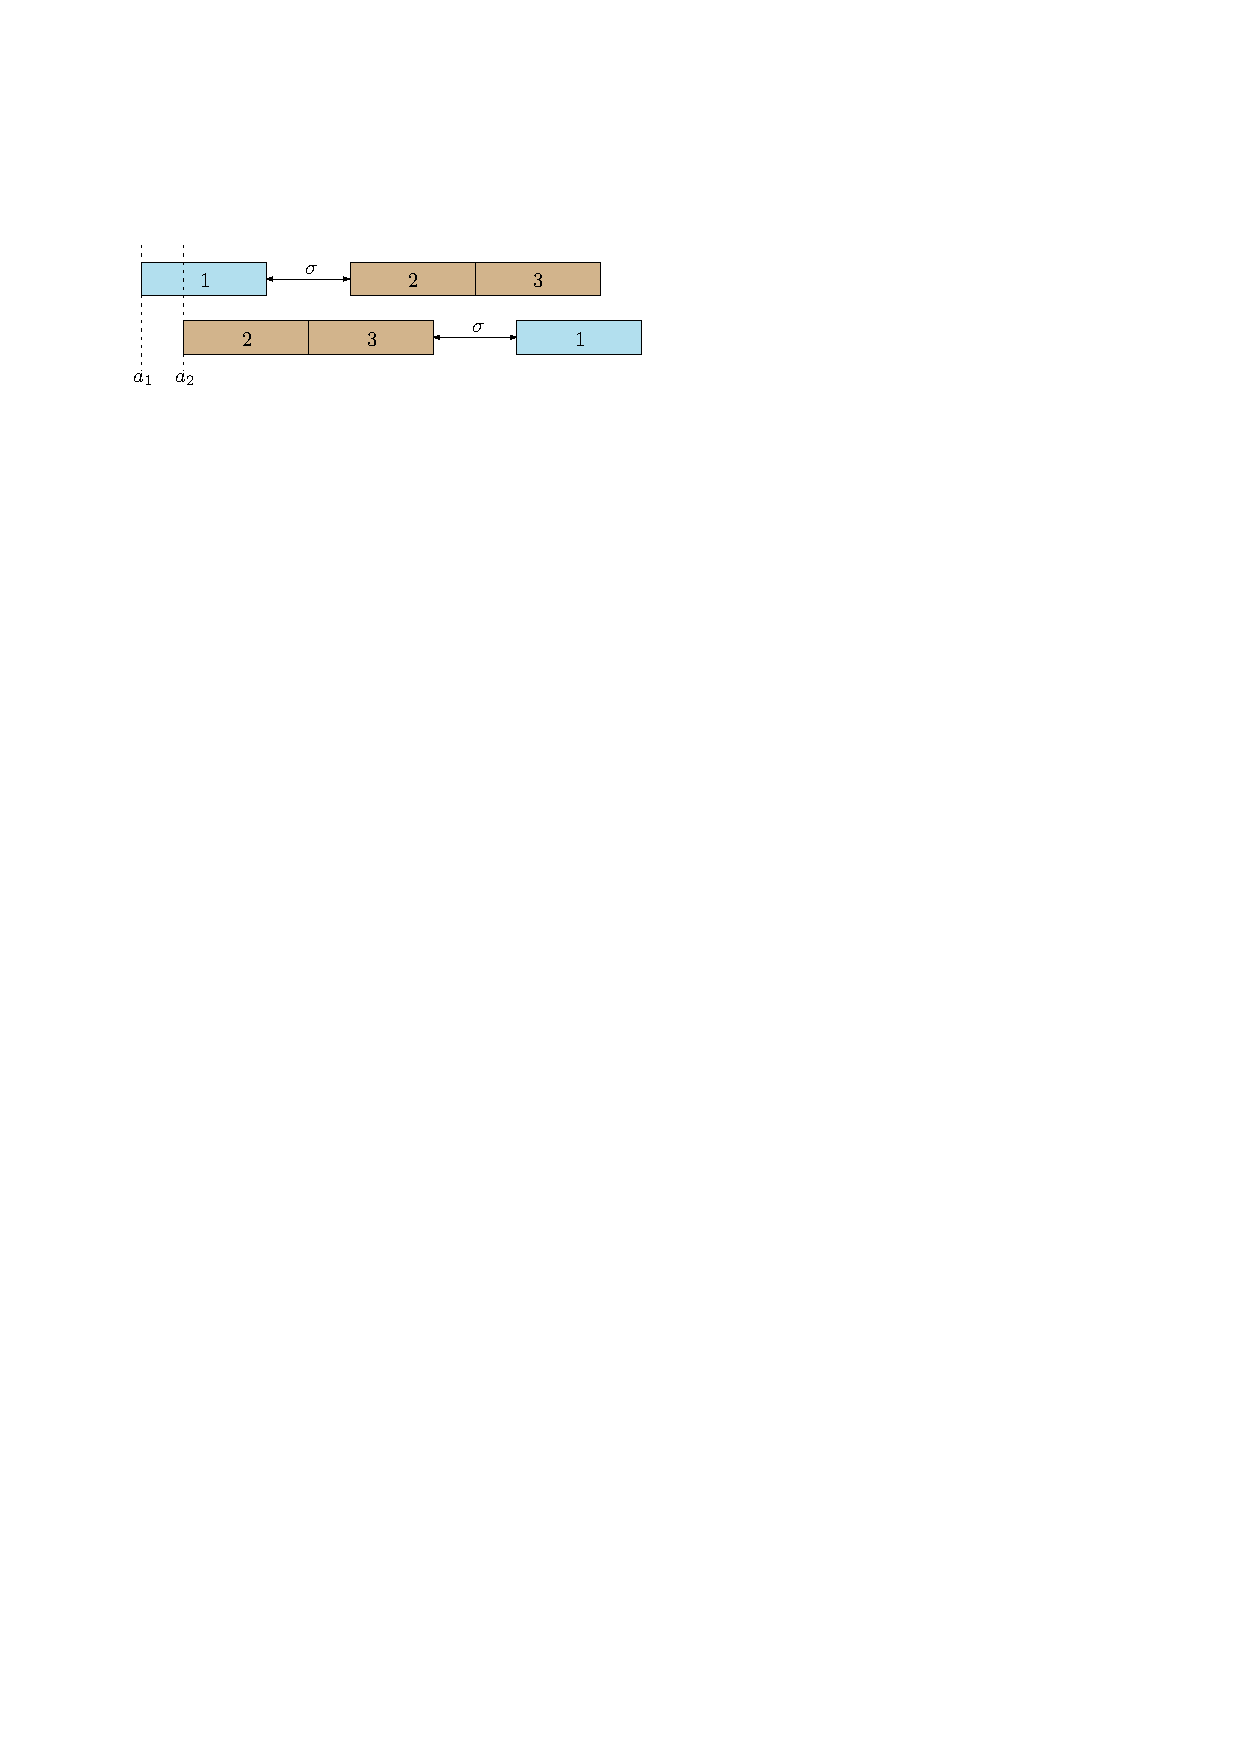
\includegraphics[width=0.55\textwidth]{figures/single/123.pdf}
  \caption{Illustration of the two possible sequences of vehicles in
    Example~\ref{example2}.}\label{fig:example2}
\end{figure}

\begin{eg}\label{example2}
  Consider two routes having one and two vehicles, see
  Figure~\ref{fig:example2}. Instead of $(1,1), (2,1), (2,2)$, we will use the
  labels $1, 2, 3$ to keep notation clear. We are interested in how the earliest
  crossing times $a_i$ influence the order of the vehicles in an optimal
  schedule. We set $a_{1} = 0$, without loss of generality, and assume that
  $a_{3} = a_{2} + \rho$. Suppose $a_{1} = a_{2}$, then we see that the order
  $2, 3, 1$ is optimal, which resembles some sort of ``longest chain first'' rule.
  Now suppose that $a_{1} < a_{2}$. For $a_{2} \geq a_{1} + \sigma$, the sequence
  $1, 2, 3$ is simply optimal. For $a_{2} < a_{1} + \sigma$, we compare the
  sequence $1, 2, 3$ with $2, 3, 1$, which are illustrated in Figure~\ref{fig:example2}. The
  first has $\sum_{i} y_{i} = \sigma + (\sigma+\rho) = 3\rho + 2\delta$, while the second sequence
  has
  $\sum_{i} y_{i} = a_{2} + (a_{2} + \rho) + (a_{2} + 2\rho + \delta) = 3 a_{2} + 3\rho + \delta$.
  Therefore, we conclude that the second sequence is optimal if and only if
  \begin{align}
    \label{eq:before-condition}
    a_{2} \leq \delta/3 ,
  \end{align}
  which roughly means that the ``longest chain first'' rule becomes optimal
  whenever the earliest crossing times are ``close enough''.
\end{eg}

In this example, we see that it does not make sense to schedule vehicle 1
between vehicles 2 and 3, because that would add unnecessary switch-over time
$\delta$. This raises the natural question whether splitting such \textit{platoons} of
vehicles is ever necessary to achieve an optimal schedule. To answer this
question, let us first give a precise definition of platoons, before slightly
generalizing the example.
%
\begin{define}
  A sequence of consecutive vehicles $(r, l+1), (r, l+2), \dots, (r, l+n)$ from
  some route $r$ is called a \textit{platoon} of size $n$ if and only if
  \begin{align}
  a_{(r,k)} + \rho = a_{(r, k+1)}  \quad \quad \text{ for all } l < k < l + n.
  \end{align}
 We say that the platoon is \textit{split}
  in some schedule $y$, if
  \begin{align}
  y_{(r, k)} + \rho < y_{(r, k + 1)} \quad \quad \text{ for some } l < k < l + n.
  \end{align}
\end{define}
%
\begin{eg}
  \label{example3}
  Suppose we have two routes $\mathcal{R} = \{ A, B \}$, each having exactly one
  platoon, denoted as $P_{A} = ((A,1), \dots, (A,n_{A}))$,
  $P_{B} = ((B,1), \dots, (B,n_{B}))$. To simplify notation, we write
  $a_{A} = a_{(A,1)}$ and $a_{B} = a_{(B,1)}$. We assume $a_{A} = 0$, without
  loss of generality, and suppose that $n_{A} < n_{B}$ and
  $a_{A} \leq a_{B} < n_{A}\rho + \delta$. Consider the ways the two platoons
  can merge by splitting A. Let $k$ denote the number of vehicles of platoon A
  that go before platoon B and let $\sum y_{i}(k)$ denote the corresponding
  sum of crossing times. See Figure~\ref{fig:example3} for an illustration of the
  situation in case of $a_{A} = a_{B}$. For $0 < k \leq n_{A}$, we have
  \begin{align*}
    \sum_{i \in \mathcal{N}} y_{i} (k) = \max\{ \delta, a_{B} - k\rho\} (n_{B} + n_{A} - k) + \delta (n_{A} - k) + \sum_{j=1}^{n_{A}+n_{B}} (j-1) \rho ,
  \end{align*}
  so when platoon A goes completely before platoon B, we get
  \begin{align}
    \sum_{i \in \mathcal{N}} y_{i} (n_{A}) = \delta n_{B} + \sum_{j=1}^{n_{A}+n_{B}} (j-1) \rho ,
    \label{eq:A-before-B}
  \end{align}
  since $\max\{ \delta, a_{B} - n_{A} \rho \} = \delta$ by the assumption on $a_{B}$. It is
  easily seen that we have $\sum y_{i}(k) > \sum y_{i} (n_{A})$ for $0 < k < n_{A}$,
  so in other words, if we decide to put at least one vehicle of platoon A
  before platoon B, it is always better to put all of them in front. As we will
  see after this example, this principle holds more generally.

  For $k=0$, so when we schedule platoon A completely after platoon B, the total
  completion time becomes
  \begin{align*}
    \sum_{i \in \mathcal{N}} y_{i} (0) = a_{B} (n_{A} + n_{B}) + \delta n_{A} + \sum_{j=1}^{n_{A}+n_{B}} (j-1) .
  \end{align*}
  Comparing this to~\eqref{eq:A-before-B}, we conclude that placing B in front
  is optimal whenever
  \begin{align*}
    a_{B} \leq (n_{B} - n_{A}) \delta / (n_{A} + n_{B}) ,
  \end{align*}
  which directly generalizes the condition~\eqref{eq:before-condition} that we
  derived for the case with $n_{A} = 1$ and $n_{B} = 2$. (end of example)
\end{eg}

\begin{figure}
  \centering
  % 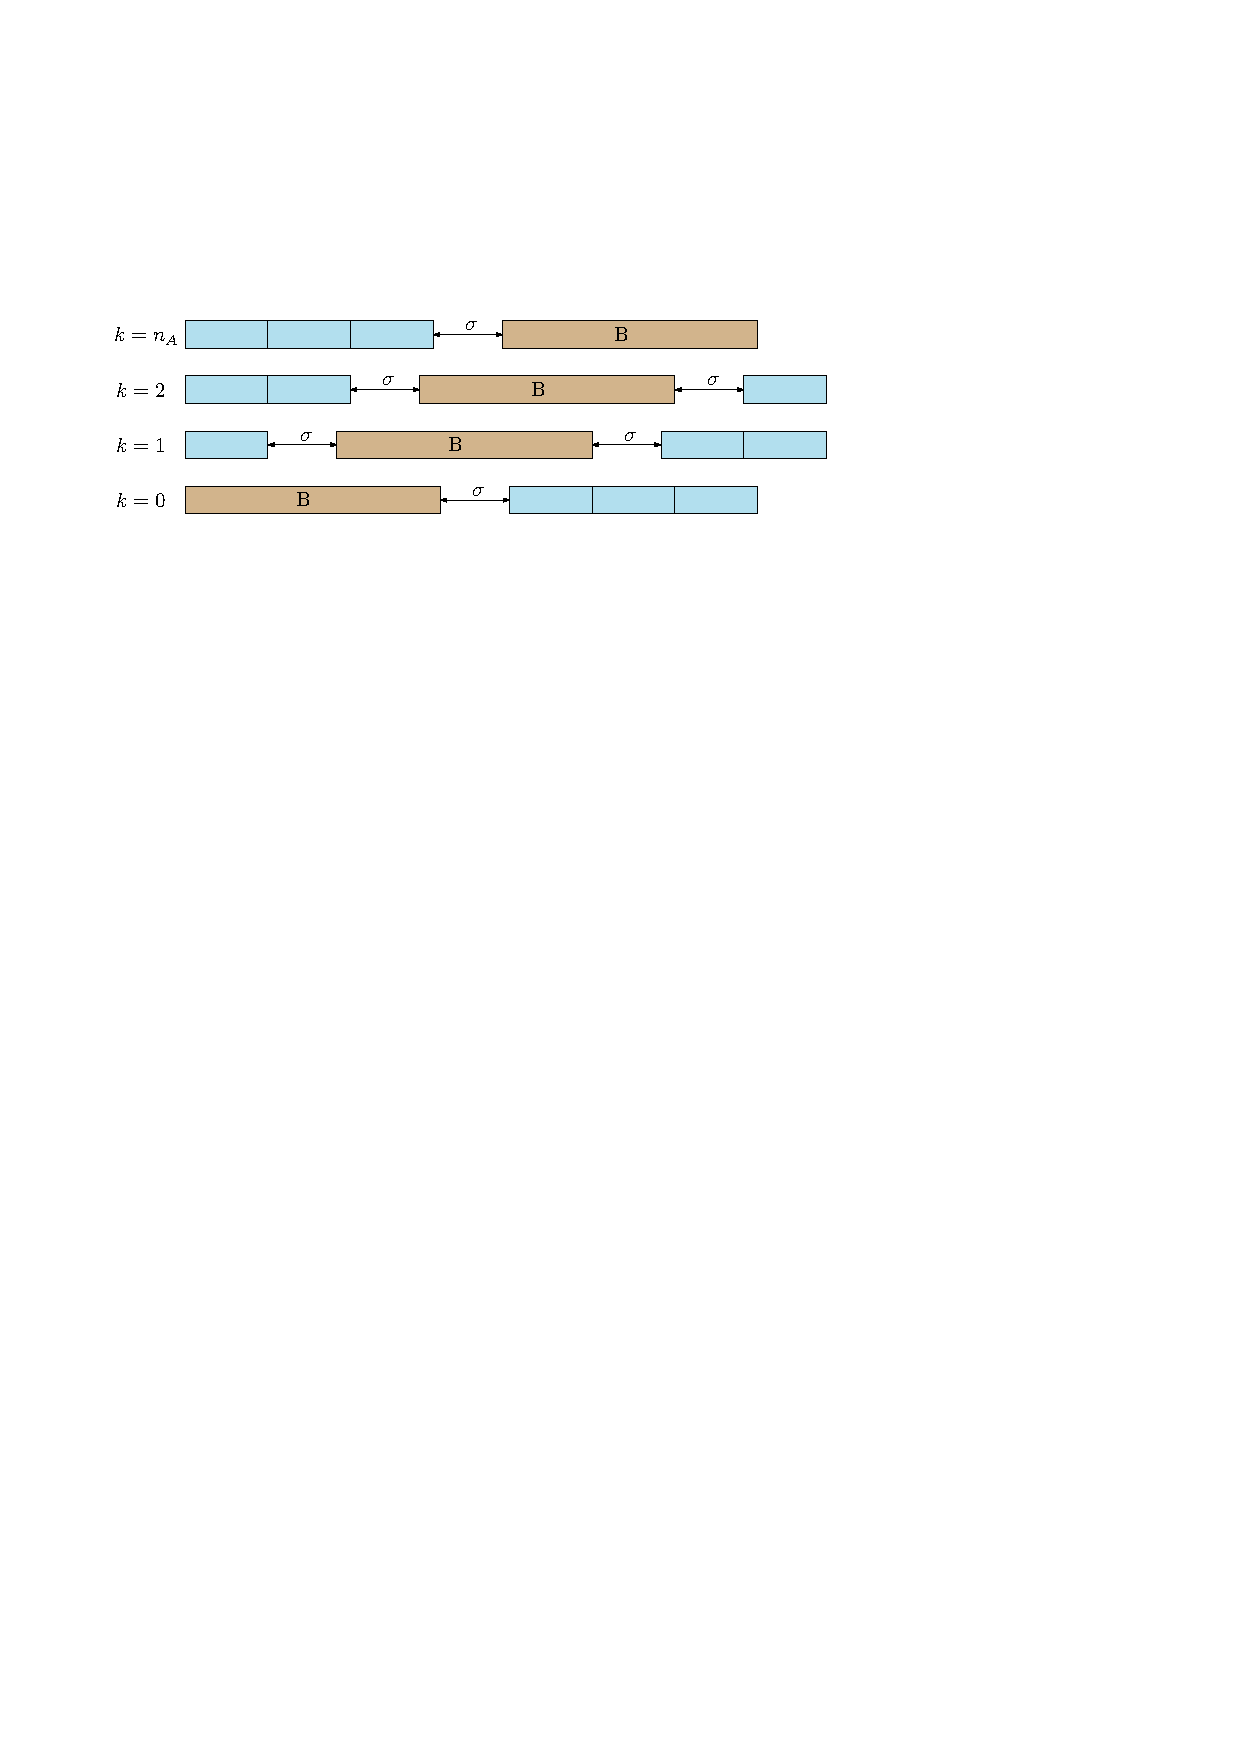
\includegraphics[width=0.8\textwidth]{figures/single/platoons.pdf}
  \includegraphics[width=0.8\textwidth]{figures/single/platoons-color.pdf}
  \caption{Different ways to split platoon A (in blue), regarding Example~\ref{example3},
    assuming equal earliest crossing times $a_{A} = a_{B}$ with $n_{A} = 3$
    vehicles in platoon A and some arbitrary number of vehicles $n_{B}$ in
    platoon B (here 4).}
  \label{fig:example3}
\end{figure}

The example shows that, when we decide to put one vehicle of a platoon before
another platoon, it is always better to put all vehicles of the platoon in
front. In other words, whenever a vehicle can be scheduled immediately after its
predecessor, this should happen in any optimal schedule. It turns out that this
property holds more generally, as stated by the following result.

\begin{restatable}[Platoon Preservation~\cite{limpensOnlinePlatoonForming2023}]{theorem}{Exhaustive}\label{thm:exhaustive}
  If $y$ is an optimal schedule for~\eqref{eq:C},
  satisfying $y_{i^{*}} + \rho \geq a_{j^{*}}$ for some $(i^{*},j^{*}) \in \mathcal{C}$, then $j^{*}$
  follows immediately after $i^{*}$, so $y_{i^{*}} + \rho = y_{j^{*}}$.
\end{restatable}

\pagebreak[4]
\subsection{Cutting planes}
Based on the above analysis of optimal substructure, we will define three types
of cutting planes for~\eqref{eq:C'}.
%
First, we will use Theorem~\ref{thm:exhaustive} to formulate two types of cutting planes---the
idea is to incorporate this necessary condition in the integer program.
%
For every conjunctive pair $(i,j) \in \mathcal{C}$, we introduce a binary
variable $b_{ij} \in \{0, 1\}$, which must satisfy
\begin{align*}
  b_{ij} = 0 &\iff y_{i} + \rho < a_{j} , \\
  b_{ij} = 1 &\iff y_{i} + \rho = a_{j} .
\end{align*}
This can be enforced using the big-$M$ method, by adding the constraints
\begin{align*}
  y_{i} + \rho &< a_{j} + b_{ij}M ,  \\
  y_{i} + \rho &\geq a_{j} - (1 - b_{ij}) M .
\end{align*}
Now observe that the statement of Theorem~\ref{thm:exhaustive} applied to $(i,j)$ is equivalent
to the inequality
\begin{align}
  y_{i} + \rho &\geq y_{j} - (1 - b_{ij}) M \tag{conj.cut} .
\end{align}
We refer to these cutting planes as \textit{necessary conjunctive cutting planes}.

Using the definition of $b_{ij}$, we can derive a second type of cutting planes
on the disjunctive decision variables $\gamma$. Whenever $b_{ij} = 1$, Theorem~\ref{thm:exhaustive}
implies that we have $i \rightarrow k$ and $j \rightarrow k$ for every other vehicle
$k \in \mathcal{N}$ on a different route $r(k) \neq r(i) = r(j)$, which can be
enforced by adding the constraints
\begin{subequations}
\begin{align}
  b_{ij} + (1 - \gamma_{ik}) + \gamma_{jk} \leq 2 , \tag{disj.cut.1} \\
  b_{ij} + \gamma_{ik} + (1 - \gamma_{jk}) \leq 2 . \tag{disj.cut.2}
\end{align}
\end{subequations}
We will refer to these as the \textit{necessary disjunctive cutting planes}.

The last type of cutting plane is related to some kind of redundancy in the
encoding of feasible crossing orders.
%
Observe that the constraints $y_i + \rho \leq y_j$ cause a fixed order of
crossing for all vehicles on the same routes. Hence, let $\mathit{pred}(i)$
denote the set of all vehicles on route $r(i)$ that cross the intersection
strictly before vehicle $i$ and let $\mathit{succ}(i)$ denote those that cross
strictly later, so we have
\begin{align*}
  \mathit{pred}(i) := \{ (r(i), k) : k > k(i) \} , \\
  \mathit{succ}(i) := \{ (r(i), k) : k < k(i) \} .
\end{align*}
%
Suppose we have some solution $(y,\gamma)$ that satisfies $\gamma_{ij} = 0$ for
some conflict pair $(i,j) \in \bar{\mathcal{D}}$, so $i \rightarrow j$, then it is
clear that $\gamma$ must also satisfy
\begin{align*}
  \gamma_{pq} = 0 \quad (\text{so } p \rightarrow q) \quad \text{ for all } \, p \in \mathit{pred}(i), \, q \in \mathit{succ}(j) .
\end{align*}
Using the big-$M$ method, we can equivalently encode this as
\begin{align}
  \sum_{\substack{p \in \mathit{pred}(i)\\ q \in \mathit{succ}(j)}} \gamma_{pq} \leq \gamma_{ij} M . \tag{trans.cut}
\end{align}
Every feasible $(y,\gamma)$ must satisfy the above inequality for every
$(i,j) \in \bar{\mathcal{D}}$, so we can safely add them to~\eqref{eq:C'}
without changing the problem. We refer to these inequalities as the
\emph{transitive cutting planes}.

\subsection{Runtime benchmark}\label{sec:runtime-bench}

We conclude this section with an evaluation of the running time of the
branch-and-bound approach.
%
Since the running time is primarily determined by the total number of vehicles
in the system, we consider problem instances with two routes and report
running times as a function of the number of vehicles per route.
%
Problem instances are generated with fixed $\rho=1.2$ and $\sigma=1.7$ and randomly
generated earliest crossing times $a_i$.
%
A detailed discussion of the distribution of $a_i$ that we used is deferred to
the end of the next chapter, where a more extensive comparison will be provided.

To keep the total computational effort within reasonable limits, we impose a
time limit of 60 seconds per instance.
%
Some care must be taken when interpreting the average running time, because some
observations correspond to cases when the time limit is reached.

For this benchmark, we used the Gurobi solver version 11.0.2 on a system with a
13th Gen Intel i5-13600K CPU and 32GiB of RAM.
%
Figure~\ref{fig:running_time} shows the average running time for the three types of cutting planes.
Observe that the necessary conjunctive cutting planes provide the most
significant runtime improvement.

% \begin{figure}
%   \centering
%   \includegraphics[scale=1]{../single/figures/milp-benchmark.pdf}
%   \caption{\note{[current figure is placeholder]} The average running time of
%     the branch-and-cut procedure is plotted as a function of the number of
%     arriving vehicles per route, for each of the three indicated cutting planes.
%     Each average is computed over $20$ problem instances. All instances use
%     $\rho = 1.2$ and $\sigma = 1.7$. The earliest crossing times for vehicles are generated
%     using the bimodal exponential interarrival time model from
%     Section~\ref{sec:results} with parameters $p=0.5, \mu_{s} = 0.1, \mu_{l} = 10$.
%     This figure clearly shows that the conjunctive cutting planes provide the
%     most runtime improvement. \note{[Why not show the case without any cutting
%       planes? Because this takes sooo much time. What we could do is give some
%       idea of this for up to 10 arrivals per route.]}}
%   \label{fig:running_time}
% \end{figure}

% choose disjunctive constraints -> linear program
\section{Route order optimization}\label{sec:sequence-representation}

In Chapter~\ref{chap:single-learning}, we will present a way to use machine learning methods to
solve the crossing time scheduling problem~\eqref{eq:C}.
%
To enable the approach there, we will first show that there exists a more
compact representation of optimal schedules: \emph{they can actually be
  represented as a sequence of route indices}.
%
This allows us to formulate the scheduling problem in terms of a particularly
simple sequential decision problem. We will make this precise in~\Cref{sec:MDP},
where we will define this in terms of a Markov decision process, that we can try
to solve with existing reinforcement learning methods.

For ease of reference, let us restate the MILP reformulation we derived above
\begin{equation}\tag{$\mathrm{C}^\prime$}
\renewcommand{\arraystretch}{1.2}
\begin{NiceArray}{ r l @{} >{{}}c<{{}} @{} l @{} }
  \displaystyle \min_{y,\gamma} & \displaystyle \sum_{i \in \mathcal{N}} y_{i} \\
  \text{s.t. } \; & a_{i} \leq y_{i} && \quad \text{ for all } i \in \mathcal{N} , \\
  & y_{i} + \rho \leq y_{j} && \quad \text{ for all } (i,j) \in \mathcal{C} , \\
  & y_{i} + \sigma \leq y_{j} + \gamma_{ij}M  &&  \\
  & y_{j} + \sigma \leq y_{i} + (1 - \gamma_{ij})M \hspace*{1.8em} && \quad \text{ for all } (i,j) \in \bar{\mathcal{D}} . \\
  & \gamma_{ij} \in \{0, 1\}
\CodeAfter\SubMatrix.{4-1}{6-2}\}
\end{NiceArray}
\end{equation}
% introduce sequence representation
Observe that this problem has infinitely many feasible solutions, because the
decision variables $y_i : i \in \mathcal{N}$, representing the crossing
times, are real-valued.
%
We will show that there is a finite representation of optimal solutions.

Recall that the binary variables $\gamma_{ij}$ encode the order in which all vehicles
cross the intersection, to which we will simply refer as the \emph{crossing
  order}.
%
We essentially show that the crossing order contains all the necessary
information to encode each optimal solution $y$.
%
Specifically, after fixing some crossing order by setting binary variables
$\gamma_{ij}$, we obtain a linear program, which can be shown to have a unique
solution whenever it is feasible.
%
However, not all settings of $\gamma_{ij}$ lead to a feasible linear program,
because some assignments correspond to chains of inequalities.
%
To make this more precise, it will be convenient to introduce the \emph{disjunctive graph}
representation, which is a common formalism used to encode scheduling problem
instances and candidate solutions.

% introduce disjunctive graph
\subsection{Disjunctive graph}

Suppose we are given some instance $(a, \rho, \sigma)$ of
problem~\eqref{eq:C}.
%
The idea of the disjunctive graph representation is to encode each of the
inequality constraints in~\eqref{eq:C'} as a weighted arc in a directed graph.
%
For each vehicle $i \in \mathcal{N}$, the earliest crossing time constraint
  $a_i \leq y_i$
is encoded by introducing a dummy node $i' \in \mathcal{N}'$ and introducing a
directed arc $i' \rightarrow i$ with weight $w(i', i) := 0$.
%
Let $\mathcal{N}' := \{ i' : i \in \mathcal{N}\}$ denote the set of all dummy
nodes and let $\mathcal{C}'$ denote the set of all dummy arcs.
%
For each pair $(i,j) \in \mathcal{C}$, the conjunctive constraint
  $y_i + \rho \leq y_j$
is encoded by a so-called \emph{conjunctive arc} $i \rightarrow j$ with weight
$w(i,j) := \rho$.
%
Lastly, recall that the the remaining constraints encode that we want exactly
one of the constraints $y_i + \sigma \leq y_j$ or $y_j + \sigma \leq y_i$ to
hold for each conflict $\{i,j\} \in \mathcal{D}$.
%
In the disjunctive graph, we model this as choosing between the
\emph{disjunctive} arcs $i \rightarrow j$ or $j \rightarrow i$, each having
weight $w(j,i) = w(i,j) := \sigma$.
%
This leads to the formal definition below.

\begin{figure}
  \centering
  \includegraphics[scale=1.0]{figures/single/disjunctive_graph_intro.pdf}
  \caption{Illustration of disjunctive graph for some instance with $R=2$
    routes, and $N=7$ vehicles in total, with $n_{1} = 3$ on the first route and
    $n_{2} = 4$ on the second route. Dummy nodes are not shown to keep the
    figure clean. The horizontal solid arrows represent the conjunctive arcs,
    the three other solid arrows represent some partial choice $\mathcal{O}$, so
    the remaining dashed lines represent pairs of disjunctive arcs that are not
    chosen.}\label{fig:disjunctive-graph-intro}
\end{figure}

\begin{define}
  Let $\omega=(a, \rho, \sigma)$ be some given instance of
  problem~\eqref{eq:C} and let $\mathcal{O} \subset \mathcal{N}^2$ be a
  \emph{selection} of disjunctive arcs such that
  \begin{align}\tag{dg.1}
    (i,j) \in \mathcal{O} \implies (j, i) \notin \mathcal{O} , \quad \text{ for all } \{i,j\} \in \mathcal{D} .
  \end{align}
  %
  The \emph{disjunctive graph of $\omega$ with respect to $\mathcal{O}$} is defined
  as the weighted directed graph
  \begin{align}\tag{dg.2}
    \mathcal{G}^\omega(\mathcal{O}) := (\mathcal{N} \cup \mathcal{N}', \mathcal{C} \cup \mathcal{C}' \cup \mathcal{O}, w) .
  \end{align}
  %
  The graph $\mathcal{G}_0^\omega := \mathcal{G}^\omega(\varnothing)$ is called the
  \emph{empty disjunctive graph} for $\omega$.
  %
  When $\mathcal{O}$ is some \emph{complete selection}, which is when
  \begin{align}\tag{dg.3}
    (i,j) \notin \mathcal{O} \implies (j, i) \in \mathcal{O},  \quad \text{ for all } \{i,j\} \in \mathcal{D} ,
  \end{align}
  then we call $\mathcal{G}^\omega(\mathcal{O})$ a \emph{complete disjunctive graph}
  for $\omega$.
  %
  If $\mathcal{O}$ is neither empty nor complete, then
  $\mathcal{G}^\omega(\mathcal{O})$ is called a \emph{partial disjunctive graph} for
  $\omega$.
\end{define}

Figure~\ref{fig:disjunctive-graph-intro} shows a partial disjunctive graph for
some small example instance. Furthermore, when the particular instance is clear
from the context or left unspecified, we will drop the $\omega$ superscript to keep
notation simple.


\subsection{Reducing the space of feasible schedules}

Suppose we fix some selection of disjunctive arcs $\mathcal{O}$, not
necessarily complete, and discard all disjunctive inequality constraints whose
arcs are not in $\mathcal{O}$, then we obtain the following linear program

\begin{equation}\label{eq:active_schedule}\tag{AS}
\begin{alignedat}{3}
  \min_{y} \quad & \sum_{i \in \mathcal{N}} y_{i} \\
  \text{s.t.} \quad & a_{i} \leq y_{i} && \quad \text{ for all } i \in \mathcal{N}, \notag \\
                 & y_{i} + \rho \leq y_{j} && \quad \text{ for all } (i,j) \in \mathcal{C}, \notag \\
                 & y_{i} + \sigma \leq y_{j} && \quad \text{ for all } (i,j) \in \mathcal{O} . \notag
\end{alignedat}
\end{equation}
We emphasize that when the selection $\mathcal{O}$ is complete, this linear
program corresponds directly to an assignment of binary variables $\gamma_{ij}$, so
that it is equivalent to~\eqref{eq:C'}.
%
Observe that the set of feasible solutions of this linear program can
equivalently be characterized using the disjunctive graph as follows.
%
Let $\mathcal{N}^{-}(j)$ denote the set of all \emph{in-neighbors} of some node
$j$ in graph $\mathcal{G}(\mathcal{O})$, which are all nodes $v \in \mathcal{N}$ such that
there is some arc $v \rightarrow j$.
%
Crossing time schedule $y$ is a feasible solution to~\eqref{eq:active_schedule} if and only if it
satisfies
\begin{align}\label{eq:feasible-schedule}
    y_j \geq \max_{i \in \mathcal{N}^{-}(j)} y_i + w(i,j)
    \quad \text{ for all } j \in \mathcal{N} .
\end{align}

\begin{define}\label{def:active}
  If schedule $y$ satisfies~\eqref{eq:feasible-schedule} with equality, it is called an
  \emph{active schedule}.
\end{define}
%
% Whenever~\eqref{eq:active_schedule} is feasible, it it clear from the objective
% that the optimal solution must be an active schedule.

Next, we investigate when a selection of disjunctive arcs guarantees
feasibility of~\eqref{eq:active_schedule}.
%
To see why feasibility is not guaranteed per se, consider some selection of
disjunctive arcs $\mathcal{O}$ such that the disjunctive graph $\mathcal{G}(\mathcal{O})$
contains some cycle
\begin{align*}
 i_1 \rightarrow i_2 \rightarrow \dots \rightarrow i_n \rightarrow i_1,
\end{align*}
%
then it is easy to see that this corresponds to the chain of inequalities
\begin{align*}
  y_{i_1} + w(i_1,i_2) &\leq y_{i_2} ,\\
  y_{i_2} + w(i_2,i_3) &\leq y_{i_3} ,\\
  &\vdotswithin{=} \notag \\[0.3em]
  y_{i_n} + w(i_n,i_1) &\leq y_{i_1} ,
\end{align*}
%
which together imply that $y_{i_1}$ must satisfy
\begin{align*}
  y_{i_1} + \sum_{m=1}^{n-1} w(i_m, i_m+1) + w(i_n, i_1) \leq y_{i_1} ,
\end{align*}
which is an obvious contradiction when we assume that $\rho$
and $\sigma$ are positive, such that all the weights in the above
inequality are positive.
%
This shows that the absence of cycles in $\mathcal{G}(\mathcal{O})$ is necessary
for feasibility of~\eqref{eq:active_schedule}. It is not surprising that it is actually also
sufficient.
%
Specifically, we show that when $\mathcal{G}(\mathcal{O})$ is acyclic, there exists an
active schedule, so~\eqref{eq:active_schedule} is feasible in that case.
%
For brevity, we will say ``$\mathcal{O}$ is acyclic'' to mean ``$\mathcal{G}(\mathcal{O})$
is acyclic''.
%
We first recall the following elementary property of directed acyclic graphs,
whose proof can be found in Appendix~\ref{app:misc}.

\begin{restatable}{proposition}{minimalnode}\label{lemma:minimal-node}
  Let $\mathcal{G}$ be some Directed Acyclic Graph (DAG) over nodes $V$, then
  there exists some $v \in V$ that has no incoming arcs, which is called
  \emph{minimal}. Moreover, the nodes $V$ can be arranged in a sequence
  $v_1, v_2, \dots, v_{|V|}$ such that if $\mathcal{G}$ contains an arc
  $v_i \rightarrow v_j$ then $i < j$. Such a sequence is called a
  \emph{topological order}.
\end{restatable}

\begin{lemma}\label{lemma:unique-active-schedule}
  Let $\mathcal{O}$ be an acyclic selection, then there exists a unique active
  schedule $y(\mathcal{O})$.
\end{lemma}
\begin{proof}
  Since $\mathcal{G}(\mathcal{O})$ is acyclic, Proposition~\ref{lemma:minimal-node} gives us
  some topological order $v_1, v_2, \dots, v_{2N}$.
  %
  Observe that there are exactly $N$ minimal nodes in
  $\mathcal{G}(\mathcal{O})$, which are precisely the dummy nodes
  $\mathcal{N}'$, for which we will use the notational convention that
  $y_{i'} := a_i$, for each $i \in \mathcal{N}$.
  %
  Next, we visit the nodes $\mathcal{N}$ in their topological order
  $v_{N+1}, \dots, v_{2N}$ and for each visited node $v$, we set
  \begin{align}
    \label{eq:y-update}
   y_{v} := \max_{u \in \mathcal{N}^-(v)} y_{u} + w(u,v) .
  \end{align}
  Every time we perform this update, note that each in-neighbor
  $u \in \mathcal{N}^-(v)$ has been visited before, because the fact that arc
  $u \rightarrow v$ exists means that $u$ appears before $v$ in the topological order.
  Therefore, $y_{u}$ has already been assigned a value so the right-hand side
  of~\eqref{eq:y-update} is well-defined. Hence, we obtain the unique schedule
  $y(\mathcal{O}) = \{ y_i : i \in \mathcal{N} \}$ satisfying~\eqref{eq:feasible-schedule} with equality.
\end{proof}

We emphasize that the lemma does not require $\mathcal{O}$ to be complete.
Observe that adding more disjunctive arcs to $\mathcal{O}$ can only cause the
crossing times in the resulting active schedule to increase. Hence, we have the
following lower bounding property of active schedules.
%
\begin{corollary}
  \label{lower-bounds}
  Let $\mathcal{O} \subseteq \mathcal{O}^*$ be two acyclic selections and let
  $y = y(\mathcal{O})$ and $y^* = y(\mathcal{O}^{*})$ denote the corresponding
  active schedules, then $y_i \leq y^{*}_i$ for all $i \in \mathcal{N}$.
\end{corollary}


Now suppose that $\mathcal{O}$ is complete, then the unique active schedule
$y(\mathcal{O})$ is the unique optimal solution to linear program~\eqref{eq:active_schedule}.
%
This means that we can use $\mathcal{O}$ to encode candidate solutions to the
original crossing time problem~\eqref{eq:C}.
%
In other words, instead of using $y_i : i \in \mathcal{N}$ as the main decision
variables, we could consider the equivalent problem of finding some acyclic
complete selection of disjunctive arcs $\mathcal{O}$, for which the
corresponding active schedule $y(\mathcal{O})$, following from~\eqref{eq:active_schedule}, is optimal.
%
This way, we essentially reduce the infinite space of candidate schedules to a
the finite space of candidate active schedules.
%
The discussion so far can be concisely summarized as:

\begin{lemma}\label{lemma:disj-graph-optimization}
  Problem~\eqref{eq:C} is equivalent to
  \begin{align}
    \label{eq:C''}
    \tag{$\mathrm{C}^{\prime\prime}$}
    \min_{\mathcal{O}} \; \sum_{i \in \mathcal{N}} y_i(\mathcal{O}) \; \text{ s.t. } \, \mathcal{O} \text{ is acylic and complete. }
  \end{align}
\end{lemma}
\begin{proof}
  When $\mathcal{O}$ is acyclic and complete, then the unique active schedule
  $y(\mathcal{O})$ is clearly a feasible solution to~\eqref{eq:C'} when setting
  $\gamma_{ij} = \mathbf{1} \{ (i,j) \in \mathcal{O} \}$.
  %
  Conversely, let $y$ be an optimal solution of~\eqref{eq:C'}. It must be an active
  schedule, otherwise some component $y_i$ is not minimal, contradicting
  optimality. Furthermore, $\gamma_{ij}$ determines an complete selection
  $\mathcal{O}$. This selection must be acyclic, otherwise there is a
  contradicting chain of inequalities in~\eqref{eq:C'}.
  %
  Hence, $\mathcal{O}$ is a feasible solution
  for~\eqref{eq:C''} such that $y = y(\mathcal{O})$.
\end{proof}

\subsection{Ordering vehicles and routes}

The disjunctive graph representation was helpful in deriving the results above,
but it is less suitable for the sequential decision making problem that we will
introduce in~\Cref{chap:single-learning}.
%
A more natural representation of the crossing order is to just consider a
permutation of vehicle indices.
%
Since the relative order of vehicles on the same route is fixed, it is even
simpler to only consider a sequence of routes.
%
This leads to the following definition.

\begin{define}
  Let $\nu \in \mathcal{V}_t$ denote a \emph{vehicle order} of length $t$,
  which is some sequence $\nu_{1:t} = (\nu_1, \nu_2, \dots, \nu_t)$ such that for each
  $t_1 \leq t_2$, we have
  \begin{align}\label{eq:order-respecting}
    r(\nu_{t_1}) = r(\nu_{t_2}) \implies k(\nu_{t_1}) \leq k(\nu_{t_2}) .
  \end{align}
  We refer to $\mathcal{V} := \mathcal{V}_N$ as the set of all \emph{complete}
  vehicle orders.
  %
  Similarly, let $\eta \in E_t$ denote a \emph{route order} of length $t$, which is some
  sequence $\eta_{1:t} = (\eta_1, \eta_2, \dots, \eta_t)$ such that it contain at most
  $n_r$ occurences of symbol $r$ for every route $r \in \mathcal{R}$. We refer to
  $E := E_N$ as the set of all \emph{complete} route orders.
\end{define}

The requirement~\eqref{eq:order-respecting} essentially says that the relative
vehicle order of each route must be respected.
%
Given some vehicle order $\nu \in \mathcal{V}_t$, let the route order
$\eta = \eta(\nu)$ be uniquely defined by $\eta_\tau = r(\nu_\tau)$, for every
$\tau \in \{ 1, \dots, t \}$.
%
Conversely, given some route order $\eta \in E_t$, it is easy to see that there must
also be a unique vehicle order $\nu = \nu(\eta)$ such that $\eta = \eta(\nu)$; this
vehicle order can be constructed using a simple procedure in which the routes
are visited according to the route order.\footnote{We can think of the vehicles
  $(r,1), (r,2), \dots (r,n_r)$ forming a queue. Each time we visit a route, we
  pick the next vehicle in the queue; for example, the first time we visit route
  $r$, we pick vehicle $(r, 1)$.}
%
This shows that there is a bijection between vehicle orders and route orders, so
we can use them interchangeably.

Suppose we are given some vehicle order $\nu \in E_t$, then we construct a
selection $\mathcal{O}(\nu)$.
%
We visit the non-dummy nodes according to order $\nu$ and for each node $\nu_k$,
we just pick all disjunctive arcs $\nu_k \rightarrow v$ such that
$u \in \mathcal{N}$ is on another route, so $r(\nu_k) \neq r(u)$, and we did not
visit $u$ before.
%
This way, we end up with a unique acyclic selection, which is complete if and
only if $t = N$.

\begin{remarknum}\label{rem:partial-order}
Conversely, suppose that $\mathcal{O}$ is some acyclic selection, then there is
generally not a single candidate route or vehicle order, see for example
Figure~\ref{fig:disjunctive-graph-intro}.
%
In other words, the subgraph of $\mathcal{G}(\mathcal{O})$ induced over
$\mathcal{N}$---which is a DAG---might have multiple topological orders
(Proposition~\ref{lemma:minimal-node}).
%
However, when $\mathcal{O}$ is complete, there is a unique topological order
$\nu(\mathcal{O})$, which we prove by contradiction: suppose $\nu'$ is a
topological order, $\nu' \neq \nu$, then there is at least one pair of indices
$i,j \in \mathcal{N}$ that appears in opposite orders in $\nu$ and $\nu'$, say,
$i$ appears before $j$ in $\nu$ and $j$ appears before $i$ in $\nu'$; due to the
conjunctive arcs, it follows that $r(i) \neq r(j)$, but then either
$(i,j) \in \mathcal{O}$ or $(j,i) \in \mathcal{O}$ would contradict either $\nu$
or $\nu'$.
\end{remarknum}

\begin{figure}
  \centering
  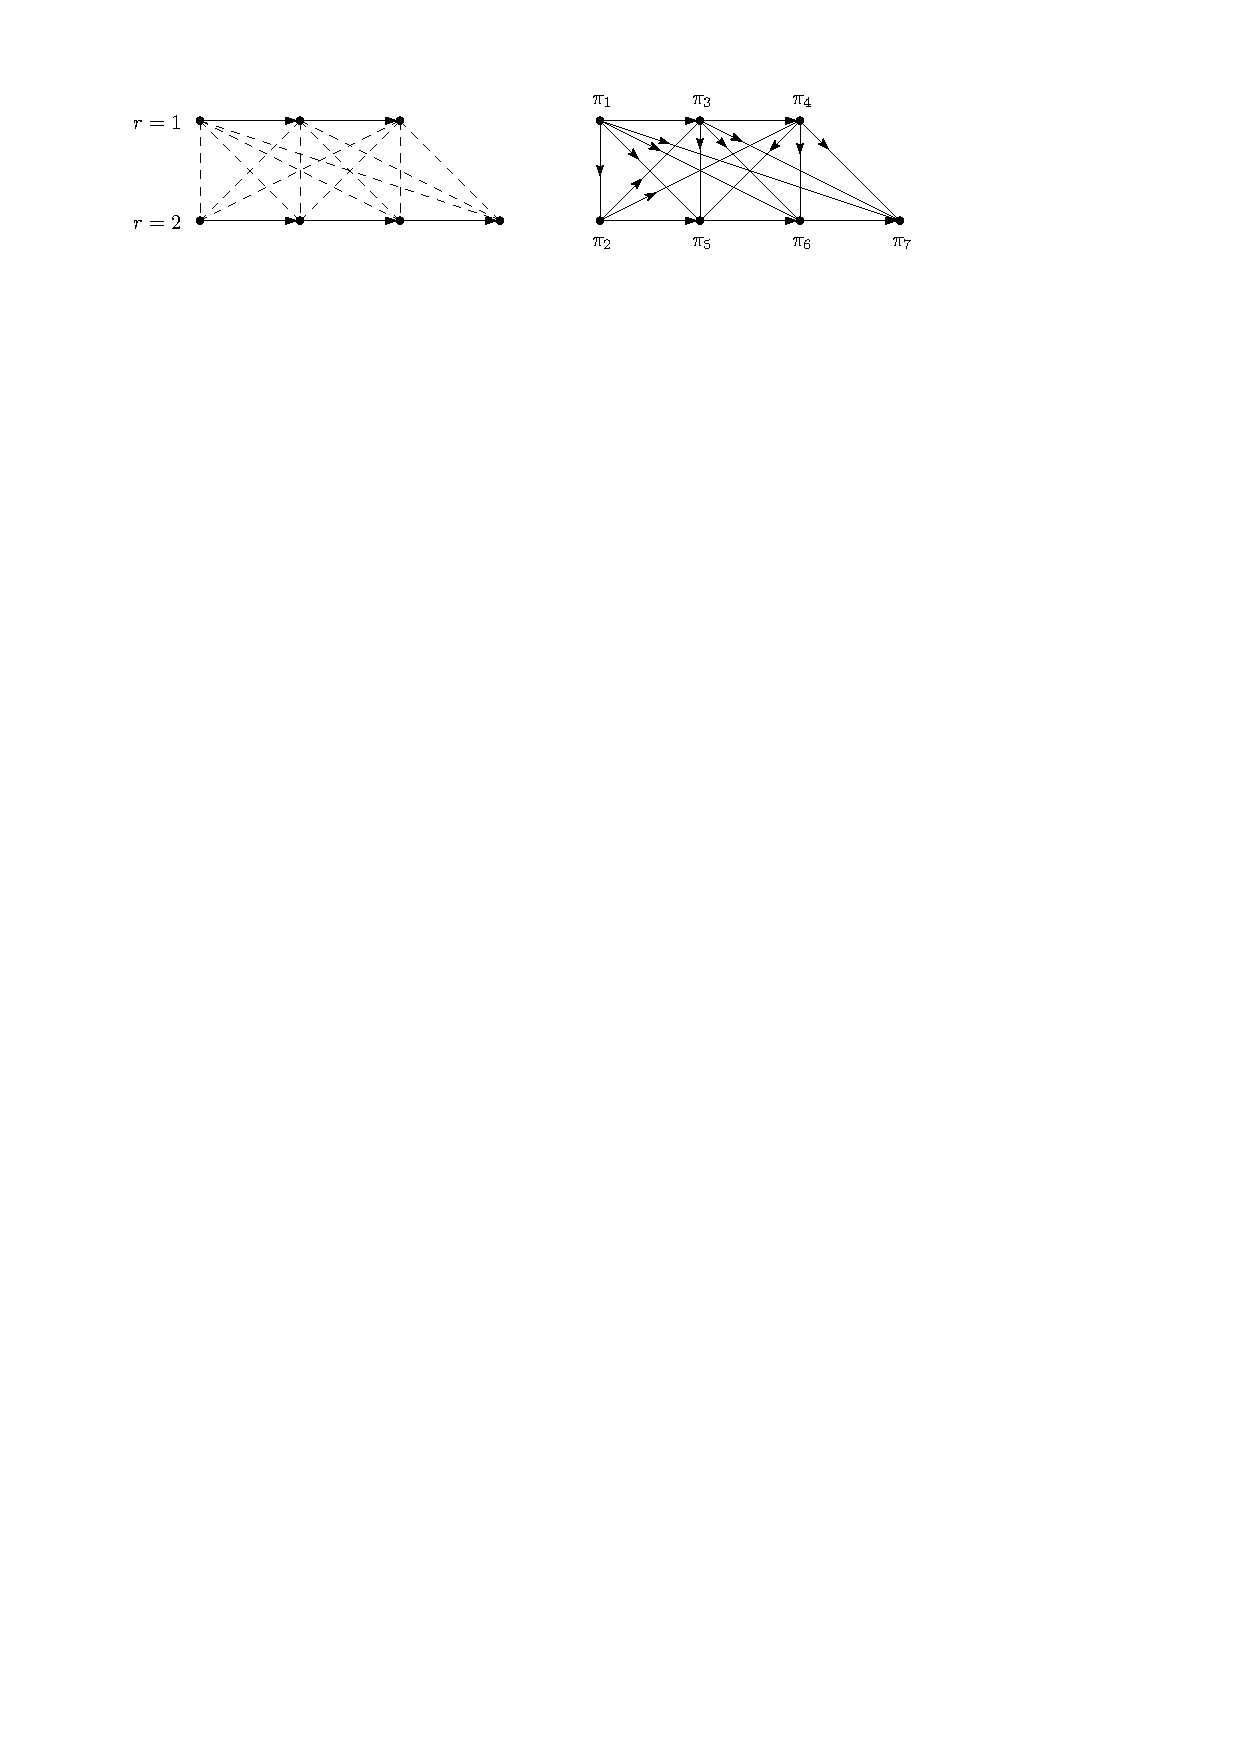
\includegraphics[width=0.98\textwidth]{figures/single/disjunctive_graph.pdf}
  \caption{Illustration of disjunctive graphs, again without dummy nodes. The
    left graph illustrates the \textit{empty} disjunctive graph with $\mathcal{O} = \varnothing$
    and $\eta = \nu = ()$. The selection shown on the right is \emph{acyclic} and \emph{complete}
    and corresponds uniquely to the vehicle order
    $\nu = ((1,1), (2,1), (1,2), (1,3), (2,2), (2,3), (2,4))$ and the route order
    $\eta = (1, 2, 1, 1, 2, 2, 2)$.}\label{fig:disjunctive-graphs}
\end{figure}

Figure~\ref{fig:disjunctive-graphs} ilustrates the above discussion by showing the three related
representations of schedules.
%
We introduce the following notation.

\begin{define}\label{def:orders}
  Let $\eta \in E_t$ be some route order, uniquely corresponding to some vehicle
  order $\nu \in \mathcal{V}_t$, uniquely corresponding to some acyclic
  selection $\mathcal{O}(\nu)$, obtained using the construction above, then we
  write $y(\eta) = y(\nu) = y(\mathcal{O}(\nu))$ to denote the corresponding unique
  active schedule.
\end{define}

\begin{theorem}
  Problem~\eqref{eq:C} is equivalent to the \emph{route ordering problem}
  \begin{align}\label{eq:D}
    \tag{$\mathrm{D}$}
    \min_{\eta \in E} \; \sum_{i \in \mathcal{N}} y_i(\eta) - a_i .
  \end{align}
\end{theorem}
\begin{proof}
  We established a bijection between $\mathcal{V}$ and $E$. Let $\Omega$ denote thet
  set of all acyclic complete selections $\mathcal{O}$. The construction above
  shows that there is also a bijection between $\Omega$ and $\mathcal{V}$.
  %
  The theorem then follows from Lemma~\ref{lemma:disj-graph-optimization} and Remark~\ref{rem:delay-objective}.
\end{proof}

% \section{Delay objective}

% After all these equivalent formulations of~\eqref{eq:C}, see
% Figure~\ref{fig:problem-relationships}, we make one more slight change to the
% problem. Until now, we have been using the total sum of crossing times as our
% objective. This captures our goal of minimizing the travel delay of vehicles
% (and it kept notation simple). From now on, we will consider the total delay,
% which is the sum of $y_i - a_i$ over all vehicles $i$.
% %
% We will spend~\Cref{chap:single-learning} on solving the following equivalent
% problem:

% \begin{mdframed}[%
%   innertopmargin=0.3em,
%   innerbottommargin=0.9em,
%   skipabove=1.5em,
%   skipbelow=4em,
% ]
% \begin{define}
%   The \emph{route ordering problem with delay objective} is defined as
%   \begin{align}
%     \label{eq:D}\tag{D}
%     \min_{\eta \in E} \; \sum_{i \in \mathcal{N}} y_i(\eta) - a_i .
%   \end{align}
% \end{define}
% \end{mdframed}

% \begin{figure}[b]
% \centering
% \def\shorten{7pt} % spacing around arrows
% \begin{tikzpicture}[
%   baseline=(T.base),
%   node distance=2.3cm,
%   every node/.style={inner sep=1pt, font=\normalsize, align=center},
%   arrow/.style={-latex, shorten >=\shorten, shorten <=\shorten},
%   equiv/.style={latex-latex, shorten >=\shorten, shorten <=\shorten},
% ]

% % nodes
% \node (T) {\eqref{eq:T*}};
% \node (UL) [right=2cm of T] {\eqref{eq:upper-level}+\eqref{eq:lower-level}};
% \node (C)  [right=2cm of UL] {\eqref{eq:C}};

% % group
% \matrix (group) [column sep=0cm, row sep=0.2cm, right=of C]
% {
% \node (Cp)  {\eqref{eq:C'}}; \\
% \node (Cpp) {\eqref{eq:C''}}; \\
% \node (RO)  {\eqref{eq:RO}}; \\
% };

% \node[fit=(Cp)(Cpp)(RO), draw=none] (groupfit) {};

% \draw[thick, decorate, decoration={brace, amplitude=4pt}]
%   ($(groupfit.south west)+(-0.0,0)$) --
%   ($(groupfit.north west)+(-0.0,0)$)
%   node[midway, left=6pt] {};

% \draw[thick, decorate, decoration={brace, amplitude=4pt, mirror}]
%   ($(groupfit.south east)+(0.0,0)$) --
%   ($(groupfit.north east)+(0.0,0)$)
%   node[midway, left=6pt] {};

% % \node (D)  [right=of Cpp] {\eqref{eq:D}};

% % arrows
% \draw[equiv] (T) -- (UL) node[midway, above=2pt, font=\footnotesize]{equiv.};
% \draw[arrow] (UL) -- (C) node[midway, above=2pt, font=\footnotesize]{reduces};
% \draw[equiv] (C) -- ($(groupfit)+(-0.8,0)$)  node[midway, above=2pt, font=\footnotesize]{equiv.};
% % \draw[equiv] ($(groupfit)+(0.8,0)$) -- (D)  node[midway, above=2pt, font=\footnotesize]{equiv.};
% \end{tikzpicture}
% \caption{Relationship between the problems of Chapters~\ref{chap:single}
%   and~\ref{chap:crossing-time-scheduling}.}\label{fig:problem-relationships}
% \end{figure}

\section{Notes and references}

A solid introduction to the algorithmic foundations for integer programming is
provided by the book~\cite{confortiIntegerProgramming2014}, whose introductory chapter also contains a clear
description of the branch-and-cut methodology. For an introduction of integer
programming with a focus on solving scheduling problems, we like to refer
to~\cite[Appendix A]{pinedoSchedulingTheoryAlgorithms2016}.
%
Note that decomposition techniques similar in nature to the decomposition of
Section~\ref{sec:bilevel} have a relatively long history in mathematical programming.
Well-known examples in the context of mixed-integer linear programming include
Dantzig-Wolfe decomposition and Benders' decomposition.\footnote{Fun fact: this
  famous method is named after Jacques
  Benders~\cite{aardalJacquesBendersHis2025}, who was a professor here at \TUE.}
%
Such techniques have been applied in air traffic scheduling~\cite{manninoPathCycleFormulation2018} and job-shop
problems arising in general traffic scheduling problems~\cite{lamorgeseNoncompactFormulationJobShop2019}.
%
Interestingly, these works also propose an alternative (``noncompact'') MILP
formulation that does not depend on the big-$M$ trick. From our current limited
understanding, this seems to be related to, and might be a better alternative to
our transitive cutting planes.

The disjunctive graph formulation is originally due
to~\cite{roy1964disjunctive}, but this technical note does not seem to be
publicly accessible via the internet.
%
This reformulation is widespread in the scheduling literature. For a little bit
more background and to see it applied to some canonical scheduling problem, we
refer the reader to the discussion of job shop scheduling in
Appendix~\ref{app:job-shop}.
%
Lemma~\ref{lemma:lb-computation} is very much related to the general notion of
an \emph{active schedule} in the scheduling literature, see~\cite[Definition
2.3.3]{pinedoSchedulingTheoryAlgorithms2016}.




\chapter{Scheduling as learning probem}\label{chap:single-learning}

We will now explain how the general ML for CO framework presented in the
previous chapter can be applied to the crossing time problem~\eqref{eq:C}.
%
As we discussed before, the most important decision is the design of the state
space of the MDP algorithm model, since this essentially determines the class of
algorithms over which we are optimizing---it is our main way of incorporating
prior knowledge and intuition into the model.
%
We will now show how our findings so far lead
to a natural choice of states and corresponding algorithmic structure.

\section{Constructive scheduling}\label{sec:MDP}
We concluded Chapter~\ref{chap:crossing-time-scheduling} by
reformulating the crossing time scheduling problem~\eqref{eq:C} as the equivalent route
ordering problem
\begin{align}
  \label{eq:D-repeat}\tag{D}
  \min_{\eta \in E} \; \sum_{i \in \mathcal{N}} y_i(\eta) - a_i ,
\end{align}
in which we try to find some valid route order $\eta \in E$ that minimizes the total
vehicle delay.
%
Given such an optimal route order $\eta^*$, we showed that the corresponding
optimal crossing time schedule $y(\eta^*)$ can be obtained by solving the linear
program~\eqref{eq:active_schedule} or by using the simple procedure described in the proof of
Lemma~\ref{lemma:unique-active-schedule}.
%
Instead of searching directly over all feasible $\eta \in E$, we propose to develop a
\emph{constructive procedure}.
% informal description
The general idea is as follows.
%
Each state encodes a \emph{partial schedule}, in which only the first few
vehicles of each route are said to be \emph{scheduled}.
%
Initially, all vehicles are unscheduled.
%
Each step corresponds to picking some route and then adding the next unscheduled
vehicle on that route to the schedule.
%
We continue until we arrive at a complete schedule.


\subsection{MDP definition}

% instance -> empty disjunctive graph
We first define the single-instance scheduling MDP, represented as the tuple
\begin{align}
  \mathcal{M}^\omega := (\mathcal{S}^\omega, \mathcal{A}^\omega, p^\omega, r^\omega) ,
\end{align}
for a single problem instance $\omega = (a, \rho, \sigma)$ for the route
ordering problem~\eqref{eq:D}.
%
We extend this to sets of instances afterwards.
%
To keep notation light, we will mostly drop the superscript $\omega$ when it is clear
from the context.

\paragraph{States and decision epochs.}
The initial state of $\mathcal{M}^\omega$ is $s_0 := (\omega, \varnothing)$. All vehicles
are said to be \emph{unscheduled} in $s_0$.
% decision epochs
The MDP has exactly $N$ decision epochs, which is equal to the total number of
vehicles in $\omega$.
%
Each intermediate state $s_t = (\omega, \eta)$ encodes some current partial route
order $\eta \in E_t$.
%
We will define the actions and transitions such that the final state
$s_N = (\omega, \eta_{1:N})$ is guaranteed to represent a complete schedule.
%
The state space is thus
\begin{align}
  \mathcal{S} = \{\omega\} \times \bigcup_{t=0}^N E_t .
\end{align}

\paragraph{Actions and transitions.}

At every decision epoch, we have to choose some route $r$ that has unscheduled
vehicles left, so the routes form the action space $\mathcal{A} = \mathcal{R}$.
%
Vehicles are added to the partial schedule according to the relative order in
which they appear on their route.
%
To make this precise, let $k_r(s_t)$ denote the number of vehicles on route $r$
that are \emph{scheduled} in state $s_t$, so initially, we have $k(s_0) = 0$.
%
Hence, the admissible actions at state $s_t$ are
\begin{align}
  \mathcal{A}(s_t) := \{ r: k_r(s_t) < n_r \} .
\end{align}
%
When we choose $r \in \mathcal{A}(s_t)$ in some state $s_t = (\omega, \eta_{1:t})$,
we simply append $r$ to the current route order to end up in $s_{t+1} = (\omega, \eta_{1:t+1})$ with $\eta_{t+1} = r$.
Let the transition function
$p : \mathcal{S} \times \mathcal{A} \rightarrow \Delta(\mathcal{S})$ be defined as
\begin{align}
  p((\omega, \eta_{1:t+1}) \mid (\omega, \eta_{1:t}), r) = \mathbf{1}\{ \eta_{t+1} = r \} .
\end{align}
%
This is a deterministic transition function, so we equivalently write
$p:\mathcal{S} \times \mathcal{A} \rightarrow \mathcal{S}$ with 
\begin{align}
  p(s_t, a) = s_{t+1} .
\end{align}

% For action $r \in \mathcal{A}(s_t)$, the first unscheduled vehicle on route $r$
% is
% \begin{align}
%   i = (r, k_r(s_t) + 1).
% \end{align}
% %
% We include vehicle $i$ in the partial schedule by adding the disjunctive arcs
% \begin{align}
%   \label{eq:disj-arcs}
%   \big\{ i \rightarrow (r', k) : r' \neq r, \;  k \in \{ k_{r'}(\mathcal{G}_t) + 1, \dots, n_{r'} \} \big\}
% \end{align}
% to $\mathcal{G}_t$ to obtain the next state $\mathcal{G}_{t+1}$.
% %
% Note that~\eqref{eq:disj-arcs} are all the disjunctive arcs from $i$ to each
% unscheduled vehicle on all other routes.

% Furthermore, since $\eta_t$ is the route that was chosen as action to arrive at
% the next partial schedule, we could write each particular transition as
% $s_{t-1} \xrightarrow{\eta_{t}} s_{t}$.

\paragraph{Final state.}
After $N$ steps, all vehicles must have been scheduled. Since the transitions
are deterministic, the final state $s_N = (\omega,\eta)$ is uniquely determined
by the sequence of actions $\eta \in E$ that were taken during the episode.
Hence, given some deterministic policy function
$\pi : \mathcal{S} \rightarrow \mathcal{A}$, let $\eta(\omega, \pi)$ denote the
unique final state that is reached by \emph{rolling out} policy $\pi$, which
means that each next action is chosen as $\eta_t = \pi(s_{t-1})$.

Given some complete route order $\eta \in E$, the quantity
\begin{align}
  R(\eta) := \sum_{i \in \mathcal{N}} a_i - y_i(\eta)
\end{align}
is a natural candidate to use as the definition of the final reward. Note that
we reversed the sign with respect to the original objective in~\eqref{eq:D}, because the
convention is that we aim to maximize reward in MDPs.
%
However, a single final reward is not convenient in practice. It is often better
for convergence of the learning algorithm when rewards happen more evenly
throughout the episode.
%
Therefore, we show how such equivalent \emph{dense rewards} can be defined in
terms of changes of certain lower bounds, which we define next.


\paragraph{Lower bounds.}
Consider some state $s_t = (\omega, \eta_{1:t})$. Let $y^\omega_i(\eta)$ be the active
schedule for instance $\omega$ with respect to route order $\eta$, as given
by~\Cref{lemma:unique-active-schedule}. Define the \emph{crossing time lower bounds}
\begin{align}
  \beta_i(s_t) = y^\omega_i(\eta_{1:t}) \quad \text{ for each } i \in \mathcal{N} .
\end{align}
%
% Given some episode of states and actions
% $\tau = (s_0, \eta_1, s_1, \dots, s_{N-1}, \eta_N, s_N)$ in the MDP, let us
% write $\beta^t_i = \beta_i(s_t)$ for each $i \in \mathal{N}$.
These values can be interpreted as providing lower bounds on the crossing times
for any \emph{completion} of the current partial schedule, as shown by the following
properties:

\begin{enumerate}[label=(\roman*)\;\;,leftmargin=3.5em,midpenalty=5]
  \item Recall that the earliest crossing times $a$ need to satisfy $a_i + \rho \leq a_j$,
        see Proposition~\ref{lemma:arrivals}. Since the empty disjunctive graph consists of only
        a single chain of conjunctive arcs per route, this implies that the
        initial lower bounds are given by
        \begin{align}
          \beta_i(s_0) = a_i \quad \text{ for all } i \in \mathcal{N}.
        \end{align}

  \item Consider some state $s_t = (\omega, \eta)$ and let $\nu = \nu(\eta)$ be the
        current vehicle order. Let $\mathcal{O}(s_t) = \mathcal{O}(\nu)$ denote
        the current acyclic selection induced by $\nu$, see
        Definition~\ref{def:orders}.
        %
        Now let $\eta^* \in E_{t^*}$ be some completion of $\eta$, so such that
        $t^* \geq t$ and $\eta^*_{1:t} = \eta$.
        %
        Observe that $s^* = (\omega, \eta^*)$ is some possible future state following
        $s_t$. Let $\mathcal{O}(\omega^*)$ denote the corresponding acyclic
        selection, then we have $\mathcal{O}(s_t) \subset \mathcal{O}(s^*)$ by
        construction. Hence, it follows from Corollary~\ref{lower-bounds} that
        we have
        \begin{align}
          \beta_i(s_t) \leq \beta_i(s^*) \quad \text{ for all } i \in \mathcal{N} .
        \end{align}

  \item Let $s_t$ be some non-initial state, so with $t \geq 1$ and let $i$ be
        the vehicle that was scheduled at step $t$, so
        $i = \nu_t =  (\eta_t, k_r(s_{t-1}) + 1)$.
        %
        Let $\omega^* \in \{s_{t+1}, \dots, s_N\}$ be some possible future state,
        then as argued in the previous point, we have
        $\mathcal{O}(s_t) \subset \mathcal{O}(\omega^*)$.
        %
        By construction, $\mathcal{O}(\omega^*)$ does not contain additional arcs
        that end in node $i$, which means that its lower bound does not change
        further:
        \begin{align}
          \beta_i(s_t) = \beta_{i}(s_{t+1}) = \dots = \beta_i(s_N) .
        \end{align}

  \item For a final state $s_N = (\omega, \eta)$, the lower bounds are the final
        active schedule
        \begin{align*}
          \beta_i(s_N) = y_i(\eta) \quad \text{ for all } i \in \mathcal{N}.
        \end{align*}

\end{enumerate}

\paragraph{Dense rewards.}
For each transition $s_{t-1} \xrightarrow{\eta_{t}} s_{t}$, we define the reward to
be
\begin{align}
  r(s_{t-1}, \eta_t, s_t) = \sum_{i \in \mathcal{N}} \beta_{i}(s_{t-1}) - \beta_{i}(s_t) .
\end{align}
Hence, for some episode
$\tau = ((\omega, \varnothing), \eta_1, s_1, \dots, s_{N-1}, \eta_N, s_N)$, which is
uniquely determined by $\eta \in E$ because $p$ is deterministic, together
with some reward sequence ${(r_t)}_{t=1}^N$, with
$r_t = r(s_{t-1}, \eta_t, s_t)$, the total episodic reward is given by the
telescoping sum
\begin{align*}
  \sum_{t=1}^{N} r_{t} &= \sum_{i \in \mathcal{N}} \sum_{t=1}^N \beta_i(s_{t-1}) - \beta_i(s_t) \\
  &= \sum_{i \in \mathcal{N}} \beta_i(s_0) - \beta_i(s_N) = \sum_{i \in \mathcal{N}} a_i - y_i(\eta) = R(\eta) ,
  % \sum_{i \in \mathcal{N}} \beta_{i}(s_0) - \beta_{i}(s_N)  = \sum_{i \in \mathcal{N}} a_{i} - y_{i}(\eta) = R(\eta) ,
\end{align*}
where we used the properties of $\beta_i$ outlined above. Hence, maximizing the
episodic reward corresponds to minimizing the delay objective of~\eqref{eq:D}.

\begin{figure}
  \centering
  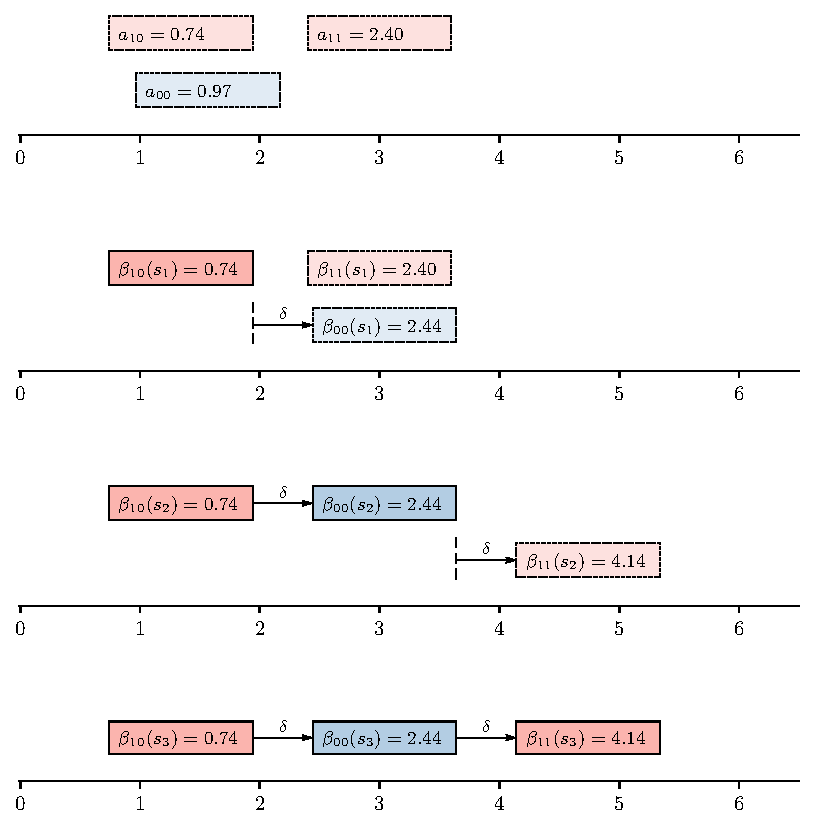
\includegraphics[scale=1]{../single/figures/episode.pdf}
  \caption{\emph{Visualizing an episode of the MDP.} Every one of the four frames in
    the figure illustrates some state $s_t$ of the MDP, by the box of vehicle
    $i$ at its current lower bound $\beta_i(s_t)$.
    %
    Hence, the first and last frame visualize the initial state of the instances
    and some possible complete schedule, respectively, in the same way as
    before. The frames in between show partial schedule states: the solid boxes
    in the top row of each frame show the current partial schedule; the
    remaining boxes in the top row show the unscheduled vehicles on the route
    that was last scheduled; the other rows show the unscheduled vehicles of the
    other routes. Note that we draw the ``switch'' arrow only for the routes other
    than the current and we draw them in the final complete
    schedule.}\label{fig:mdp-episode}
\end{figure}



\paragraph{Joining single-instance MDPs.}

Observe that the state space is a union of disjoint sets
\begin{align}
  \label{eq:8}
  \mathcal{S}^\omega = \{(\omega, \varnothing)\} \sqcup \mathcal{S}_1^\omega \sqcup \mathcal{S}_2^\omega \sqcup \dots \sqcup \mathcal{S}_N^\omega ,
\end{align}
where each $\mathcal{S}_t^\omega = \{\omega\} \times E_t$ denotes the set of all possible
partial schedules that can be obtained from $(\omega, \varnothing)$ after scheduling
exactly $t$ vehicles.
%
Further, suppose we have two distinct problem instances $\omega_1 \neq \omega_2$, then we
clearly have
\begin{align}
  \mathcal{S}^{\omega_1} \cap \mathcal{S}^{\omega_2} = \varnothing .
\end{align}
%
Given some set of instances $\mathcal{I}$ such that each $\omega \in \mathcal{I}$ has
the same set of routes $\mathcal{R}$, we can consider the following \emph{joint state space}
\begin{align}
  \mathcal{S} = \bigsqcup_{\omega \in \mathcal{I}} \mathcal{S}^\omega .
\end{align}
Therefore, let $\mathcal{A} := \mathcal{R}$ and define
$p : \mathcal{S} \times \mathcal{A} \rightarrow \Delta(\mathcal{S})$ and
$r : \mathcal{S} \times \mathcal{A} \rightarrow \mathbb{R}$ such that
\begin{align*}
  p(u, a) = p^\omega(u, a) \quad \text{ when } u \in \mathcal{S}^\omega , \\
  r(u, a) = r^\omega(u, a) \quad \text{ when } u \in \mathcal{S}^\omega ,
\end{align*}
%
then the \emph{joint constructive scheduling} MDP for $\mathcal{I}$ is
\begin{align}
  \tag{M}
  \mathcal{M}_\mathrm{constr} = (\mathcal{S}, \mathcal{A}, p, r) .
\end{align}


\paragraph{Episode visualization.}

Recall the visualization for instances and corresponding complete schedules we
introduced in the previous chapter. In order to strengthen our intuition about
the above MDP definition, we extend this type of visualization to partial
schedules such that we can visualize all steps of the MDP, which is explained in
Figure~\ref{fig:mdp-episode}.

% \begin{remark}
%   Let us show how to efficiently keep track of the lower bounds by using the
%   following partial update scheme.
%   %
%   Let $s_{t-1}$ be the current state and let $r^* = \eta_t$ denote the next action,
%   which means that vehicle $i = (r^*, k_{r^*}(s_{t-1}) + 1)$ will be added to the
%   schedule.
%   %
%   We first copy all the lower bounds from the previous state, so
%   $\beta \leftarrow \beta(s_{t-1})$.
%   %
%   For each other route $r \neq r^*$, let $j = (r, k_r(s_{t-1}) + 1)$ be the first
%   unscheduled vehicle. Because the disjunctive arc $i \rightarrow j$ gets introduced, we
%   need to update
%   \begin{align*}
%     \beta_j \leftarrow \max(\beta_j, \; \beta_i + \sigma ) .
%   \end{align*}
%   %
%   When this update did not change $\beta_j$, we say it was void. If the update was
%   not void, we only have to propagate this change along the chain of conjunctive
%   arcs starting from $j$, because these unscheduled vehicles do not have any
%   outgoing disjunctive arcs. Let such conjunctive chain be denoted by
%   $j = (r,k) \rightarrow (r,k+1) \rightarrow \dots \rightarrow (r,n_r)$, then we update
%   \begin{align*}
%     \beta_{r,l + 1} \leftarrow \max(\beta_{r,l + 1} , \; \beta_{r,l} + \rho) ,
%   \end{align*}
%   in a loop where $l$ steps from $k$ to $n_r - 1$. Once one of these updates
%   becomes void, we know that all remaining updates will also be void, so we can
%   stop and continue to the next route.
% \end{remark}

\subsection{Learning objective}

For the MDP defined above, we now define the learning objective in terms of
finding some policy $\pi$, to which the rest of this chapter is devoted.
%
Afterwards, we briefly discuss the set $\Pi$ of policies under consideration.
Concrete distributions $P$ will be defined at the end of the chapter, when we do
some numerical experiments.

\begin{mdframed}[%
  innertopmargin=0.3em,
  innerbottommargin=0.9em,
  skipabove=1.5em,
  skipbelow=4em,
]
  \begin{define}
    Given some distribution $P$ over problem instances of some class
    $\mathcal{I}$, the \emph{learning to schedule} problem is defined as
    \begin{align}\label{eq:MDP}
      \tag{MDP}
      \max_{\pi \in \Pi} \mathbb{E}_{\omega \sim P} [R(\eta(\omega, \pi))] ,
    \end{align}
    where $\eta(\omega, \pi)$ denotes the unique schedule obtained for $\omega$ by applying
    $\pi$ in $\mathcal{M}_\mathrm{constr}$ with initial state $(\omega, \varnothing)$, and where
    $R(\cdot)$ denotes the total episodic reward as defined above.
  \end{define}
\end{mdframed}

% Consider the following distinguishing feature of problem distributions.
% \begin{define}
%   When $F_r = F$ for all $r \in \mathcal{R}$, the problem distribution is called \emph{symmetric}.
% \end{define}

A common starting point is to let $\Pi$ be all stochastic policies\footnote{Even
  more general classes of policies can be considered, when we allow the next
  action to depend on the entire history of states and actions encountered so
  far. In our setting, it can be shown that this does not result in more
  powerful policies, in the sense that there always exists an optimal policy
  that is Markov, i.e, is only a function of the current state.}
$\pi : \mathcal{S} \rightarrow \Delta(\mathcal{A})$. However, since the state
space of $\mathcal{M}_\mathrm{constr}$ decomposes into finite subspaces as
sketched above, it can be shown that the following class of policies is general
enough, in the sense that it contains optimal policies.

\begin{define}
  Let $\Pi_\mathrm{p}$ be the set of \emph{pure policies}, being all functions
  $\pi : \mathcal{S} \rightarrow \mathcal{A}$.
\end{define}

\begin{theorem}
  There exists an optimal policy $\pi^*$ for $\mathcal{M}_\mathrm{constr}$ such
  that $\pi^* \in \Pi_\mathrm{p}$.
\end{theorem}
\begin{proof}[Proof (sketch)]
  For each initial state $(\omega, \varnothing)$, only a finite part
  $\mathcal{S}^\omega$ of the state space is reachable.
  %
  It is well-known that finite-state MDPs have an optimal deterministic policy
  $\pi^\omega$, which is not necessarily stationary, so it consists of a
  sequence of decision rules
  $\pi^\omega = (d^\omega_1, d^\omega_2, \dots, d^\omega_N)$.
  %
  However, since
  $\mathcal{S}^\omega = \{(\omega, \varnothing)\} \sqcup \mathcal{S}_1^\omega \sqcup \dots \sqcup \mathcal{S}_N^\omega$,
  each decision rule $d_t^\omega$ is only ever applied to states in
  $\mathcal{S}_t^\omega$, so we can safely assume
  $d_1^\omega = d_2^\omega = \dots = d_N^\omega$ without changing the final
  solution $\eta(\omega, \pi^\omega)$.
  %
  Since the state space is partitioned as
  $\mathcal{S} = \sqcup_\omega \{ \mathcal{S}^\omega \}$, we can join
  $\pi^\omega$ for each $\omega$ to obtain a pure policy $\pi$.
\end{proof}


\subsection{State space reduction}

It can be shown that the optimal completion of a partial schedule does not
depend on the vehicles that have already been scheduled, see for
example~\Cref{fig:abstract}.
%
To make this more precise, we introduce a mapping from the state space to
particular subset of \emph{abstract states}.
%
More concretely, given some partial schedule, we perform the following two
operations.
\begin{enumerate}
  \item The vehicles that have already been scheduled are discarded. We take the
        unscheduled vehicles and do a simple renumbering of their indices.
  \item It is not difficult to see that the optimal completion of a partial
        schedule is invariant to uniform time-shifts of all lower bounds.
        %
        Hence, we fix a unique reference time for the partial schedule.

  \item We subtract the reference time from the lower bound of each unscheduled
        vehicle. The resulting shifted lower bounds become the arrival times in
        a new empty instance, consisting of only unscheduled vehicles.
\end{enumerate}

\begin{figure}
  \centering
  \includegraphics[scale=1]{../single/figures/abstract.pdf}
  \caption{Two states of the constructive scheduling MDP that are equivalent
    with respect to optimal completion: it can be shown that any optimal
    completion of the above partial schedule is also optimal for the lower
    one.}%
  \label{fig:abstract}
\end{figure}

\paragraph{State abstraction.}
Let $s = (\omega, \eta)$ be some state of $\mathcal{M}_\mathrm{constr}$.
% notation
Let $\mathcal{N}(s)$ denote the index set of the problem instance and let
$n_r(s)$ and $k_r(s)$ denote the total number vehicles and the number of
scheduled vehicles on route $r$, respectively. Furthermore, let $\nu(s)$ denote
the unique vehicle order corresponding to the current route order $\eta$.


We define the \emph{abstract state mapping}
$\phi : \mathcal{S} \rightarrow \mathcal{S}$ by directly constructing $\phi(s)$.
%
The abstract state is an empty instance
$\phi(s) = ((\bar{a}, \rho, \sigma), \varnothing)$ with index set
$\bar{\mathcal{N}}(s)$.
%
We simply keep the indices of the unscheduled vehicles and renumber them to
obtain
\begin{align}
  \bar{\mathcal{N}}(s) := \{ (r,k) : r \in \mathcal{R}, \; k_r(s) + k \leq n_r(s), \; k\in\mathbb{N}^+ \} .
\end{align}
%
Let $\{ \beta_i(s) : i \notin \nu(s) \}$ be the set of lower bounds of all
unscheduled vehicles. Among these lower bounds, let $\beta^{(1)}(s)$ and
$\beta^{(2)}(s)$ denote the smallest and second smallest, respectively.
%
Define the arrivals times by time-shifting the lower bounds by
\begin{subequations}
\begin{align}
  c(s) &:= \min \{ \beta^{(1)}(s), \beta^{(2)}(s) - \delta \} , \\
  \bar{a}_i(s) &:= \beta_i(s) - c(s) \quad \text{ for all } i \in \bar{\mathcal{N}}(s) .
\end{align}
\end{subequations}


\begin{theorem}
  Let $\pi^* \in \Pi_\mathrm{p}$ be some optimal policy for~\eqref{eq:MDP}, then
  there exists some function $f : \mathcal{S} \rightarrow \mathcal{S}$ such that
  $\pi^* = f \circ \phi$.
\end{theorem}
\begin{proof}[Proof (sketch)]
  Consider a pair $s_1, s_2 \in \mathcal{S}$ such that $\phi(s_1) = \phi(s_2)$. This means that they have the same sets of admissible actions, so pick some arbitrary $a \in \mathcal{A}(s_1) = \mathcal{A}(s_2)$.
  %
  For any such $s_1, s_2$ and $a$, it can be shown that
  $r(s_1, a, p(s_1, a)) = r(s_2, a, p(s_2, a))$ and
  \begin{align*}
    \phi(p(s_1, a)) = \phi(p(s_2, a)) ,
  \end{align*}
  which shows that $\phi$ is a model-irrelevant state abstraction, see
  Definition 3 in~\cite{liUnifiedTheoryState}, then Theorem 3 of the same paper
  guarantees the existence of $f$. The same result can also be established using
  the more general framework of MDP
  homomorphisms~\cite{ravindran2001symmetries}.
\end{proof}

Next, we provide two suggestions for parameterizing $f$.

\section{Policy parameterizations}
\subsection{Platoon preserving policies}

Let $s_t$ denote the current partial schedule and assume that it is
not an initial state, so $t \geq 1$. Let the vehicle that was scheduled in the
previous step be denoted by $i^* = \nu_t = (r^*, k^*)$ and suppose $j^* = (r^*, k^*+1)$ exists.
%
By construction of the lower bounds, $\beta_{i^*}(s_t) = y_{i^*}$ is the final crossing
time of vehicle $i^*$, regardless of the remaining actions taken in the MDP.
%
Recall from~\Cref{sec:platoons} the platoon preservation
Theorem~\ref{thm:exhaustive}, which essentially says that whenever it is
possible to schedule a vehicle immediately after its predecessor on the same
route, then this must be done in an optimal schedule.
%
Therefore, the platoon preservation rule requires
\begin{align}\label{eq:rule-exhaustive}\tag{exhaustive}
  \beta_t(i^*) + \rho \geq a(j^*), \quad \text{  then next action is } r^* , 
\end{align}
where $r^* = \eta_t$ is the last scheduled route.
%
Whenever a policy $\pi$ satisfies this rule, we say that it is
\emph{exhaustive}, so the platoon preservation theorem implies that each optimal
policy $\pi^*$ must be exhaustive.


\paragraph{Threshold heuristic.}

We will propose a simple class of exhaustive policies.
%
The idea is to consider the next unscheduled vehicle of the route that was
last chosen. We aim to continue on the same route as long as
possible, to avoid introducing unnecessary switch-over time $\delta$.
%
Recall that a platoon was defined as a sequence of consecutive vehicles
$(r, l+1), (r, l+2), \dots, (r, l+n)$ from some route $r$ such that
\begin{align*}
  a(r,k) + \rho = a(r, k+1)  \quad \quad \text{ for all } l < k < l + n.
\end{align*}
%
An alternative interpretation of the platoon preservation theorem says that
platoons should be treated as a whole unit: given some other vehicle on a
different route, the platoon is either scheduled entirely before it or entirely
after it. In other words, the platoon is never \emph{split} in an optimal
schedule.

% generalize to "almost platoons"
Based on this idea, we might think that the same holds whenever a vehicle can be
scheduled \textit{sufficiently} soon after its predecessor.
%
In other words, we might relax the definition of a platoon to
\begin{align*}
  a(r,k) + \rho + \tau \geq a(r, k + 1) \quad \text{ for all } l < k < l + n,
\end{align*}
for some small \emph{threshold} parameter $\tau \geq 0$.
%
Therefore, we construct a policy that satisfies
\begin{align}\label{eq:rule-threshold}\tag{threshold}
  \text{ if } \; \beta_t(i^*) + \rho + \tau \geq a(j^*) , \; \text{ then next action is } r^* ,
\end{align}
where $r^* = \eta_t$ is again the last scheduled route.

\begin{define}
  The \emph{threshold policy} is defined as
  $\pi_\tau(s) := f_\tau(\phi(s))$, with
  
\begin{align}
  f_\tau(((\bar{a}, \rho, \sigma), \varnothing)) := \begin{cases}
    r(\argmin_i \bar{a}_i) & \text{ if } \min_i \bar{a}_i \leq \tau , \\
    r(\argmin_i \{ \bar{a}_i : \bar{a}_i \geq \delta \}) & \text{ otherwise. }
    \end{cases}
\end{align}
\end{define}

\begin{proposition}
  Policy $\pi_\tau$ satisfies~\eqref{eq:rule-threshold} and hence~\eqref{eq:rule-exhaustive}.
\end{proposition}

\paragraph{Grid search.}

Given some set of instances $D_\mathrm{train}$, we approximate the best
parameter $\tau^*$ through a simple grid search by selecting $K$ evenly spaced
$\tau_k \in [\tau_{\min}, \tau_{\max}]$ and evaluating
\begin{align*}
  \tau^* := \argmax_{\tau_k} \sum_{\omega \in D_\textrm{train}} R(\eta(\omega, \pi_{\tau_k})) .
\end{align*}
%
Alternatively, we could use some derivative-free optimization method like Brent's method.

%% without state abstraction, i.e., direct parameterization:
% Define
% \begin{align*}
%   i^{(1)}(s) &:= \argmin_{i \notin \nu(s)} \beta_i(s) , \\
%   \beta^{(1)} (s) &:= \min_{i \notin \nu(s)} \beta_i(s), \\
%   \beta^{(2)} (s) &:= \min_{i^{(1)} \neq i \notin \nu(s)} \beta_i(s), \\
%   c(s) &:= \min \{ \beta^{(1)}(s), \beta^{(2)}(s) - \delta \} , \\
%   r^{(1)}(s) &:= r(i^{(1)}(s)) , \\
%   r^{(2)}(s) &:= \argmin_r \{\beta_r : \beta_r \geq c(s) + \delta\} .
% \end{align*}
% %
% Given some threshold $\tau$, the threshold heuristic is defined as 
% %
% \begin{align}
%   \pi_\tau(s) = \begin{cases}
%     r^{(1)}(s) & \text{ if } \beta^{(1)} (s) \leq c(s) + \tau , \\
%     r^{(2)}(s) & \text{ otherwise. }
%     \end{cases}
% \end{align}
% \begin{proposition}
%   Policy $\pi_\tau$ can be written as $f \circ \phi$.
% \end{proposition}


\subsection{Differentiable policies}\label{sec:neural-param}

Instead of manually trying to develop a good parameterization of $f$, we will
weaken our prior by considering a simple neural parameterization.
%
Instead of only considering the first unscheduled vehicle on each route, we now
propose a parameterization that takes into account the sequence of relative
lower bounds of unscheduled vehicles as follows.
%
Let $\bar{n}_r$ denote the number of unscheduled vehicles in $s$, such that
$\bar{\mathcal{N}}(s)$ contains precisely $\bar{n}_r$ vehicles on route $r$,
which we denote as
%
\begin{align}
  \bar{a}_r := \{ \bar{a}_{rk} : 1 \leq k \leq \bar{n}_r \} .
\end{align}
%
Each of these \emph{route sequences} $\bar{a}_r$ is encoded by a recurrent
neural network $f^{\mathrm{RNN}}_\theta$ to produce a \emph{route embedding}
$f^{\mathrm{RNN}}_\theta(\bar{a}_r)$.
%
The concatenation of these route embeddings is fed through a fully connected
layer $f^{\mathrm{full}}_\theta$ and softmax to produce a distribution over
routes.

This means that we will explicitly consider stochastic policies, which is
numerically attractive.
%
We could call this policy the \emph{training policy} $\pi_\theta$.
%
However, note that eventually want a deterministic \emph{target policy} $\pi_\mathrm{d}$. Hence,
we need to specify how to make the training policy deterministic again. We will
use the following simple greedy action selection. Let
$\pi = f \circ \phi : \mathcal{S} \rightarrow \Delta(A)$ be some stochastic
policy, then let $\pi_\mathrm{d} : \mathcal{S} \rightarrow \mathcal{A}$ be
defined as
\begin{align} 
  \pi_\mathrm{d}(s) = \max_{a \in \mathcal{A}(s)} \pi(a | s).
\end{align}

\paragraph{Imitation learning.}

The simplest method to find $\theta$ is to use an \emph{imitation learning} approach.
%
First, we collect \emph{expert demonstration} by taking some instance from the
distribution of interest and replaying an optimal route sequence on the MDP,
while keeping track of the visited states. This results in a set of state-action
pairs for which we can consider a simple prediction task, which we will now make
precise.

Let $\mathcal{I}_\mathrm{train}$ be some set of training instances. For each
$\omega \in \mathcal{I}_\mathrm{train}$, let $\eta^\omega$ denote some optimal
route sequence, which we can be found, for example, by solving~\eqref{eq:C'},
and let $N(\omega)$ denote the total number of vehicles in $\omega$.
%
For each $\omega \in \mathcal{I}_\mathrm{train}$, we let
$\mathcal{M}_\mathrm{constr}$ start in $s_0 = (\omega, \varnothing)$ and we
replay $\eta^\omega$ to obtain the set of state-action pairs
\begin{align}
  \label{eq:2}
  \mathcal{X}_\mathrm{train} = \{ (\phi((\omega, \eta_{1:t-1})), \eta_{t}): t \in \{1, \dots, N(\omega) \} , \omega \in \mathcal{I}_\mathrm{train}\} .
\end{align}
%
We can now consider the supervised learning task of predicting the next action, given the current state.
%
For example, in the case of two route $\mathcal{R} = 2$, we can use the binary
cross entropy loss
\begin{align}
  L_\theta(\mathcal{X}_\mathrm{train}) = -\frac{1}{|\mathcal{X}_\mathrm{train}|} \sum_{(s,a) \in \mathcal{X}_\mathrm{train}} \mathbf{1}\{a = 1\} \log(\pi_\theta(1 | s)) + \mathbf{1}\{a = 2\}\log( \pi_\theta(2 | s) ) ,
\end{align}
where $\pi_\theta(a | s) \in [0,1]$ denotes probability assigned to action $a$
by the policy.



\paragraph{Policy-gradient optimization.}

The above method relies on the ability to compute optimal schedules in the first
place. For very large instances, this is not possible in reasonable time.
Therefore, it is attractive to consider a method that is based on sampling from
the MDP. These kinds of policy-gradient methods rely on the fundamental Policy
Gradient Theorem.
%
Define
\begin{align}
  J(\theta) := \mathbb{E}_{\omega \sim P}[R(\eta(\omega, \pi_\theta))] 
\end{align}
which is the expected reward of $\mathcal{M}_\mathrm{constr}$, when sampling the
initial state according to $P$.
Note that the expectation is also taken over the random actions of our training policy.
%
The policy gradient theorem essentially tells us that we can use samples of an
episode $\tau = (s_0, \eta_1, r_1, s_1, \dots, s_N, r_N)$ to estimate the gradient as
%
\begin{align}
  \nabla_\theta J(\theta) &\propto \mathbb{E}_{\omega \sim P, \tau \sim \pi_\theta} \left[ \sum_{t=0}^{N-1} \nabla_\theta \log \pi_\theta(\eta_{t+1} | s_{t}) \sum_{t'=t+1}^{N} r_{t'}  \right]  .
\end{align}

A well-known manifestations of this sampling approach is the classical REINFORCE
with baseline algorithm. However, our current purpose is not to understand the
fundamentals of policy-gradient algorithms, but rather to investigate the
feasibility of this approach in general. Hence, we will use the modern and very
popular Proximal Policy Optimization (PPO) algorithm~\cite{schulmanProximalPolicyOptimization2017}.


\clearpage
\section{Experimental results}\label{sec:results}

% performance metrics: optimality, training time, eval (inference) time
The evalutation of a computational method's performance is based on two aspects.
Of course, the quality of the produced solutions is important. Second, we need
to take into account the time that the algorithm requires to compute the
solutions. We need to be careful here, because some of our methods involve both
training time as well as inference time.
% measure generalization w.r.t. instance size and structure
Furthermore, we will evaluate generalization of learned policies along the axis
of instance size and the axis of instance structure, which will be made more
concrete next.

% instance size
\paragraph{Instance size.}
Assume that parameters $\rho$ and $\sigma$ are fixed globally.
%
For some set of instances $\mathcal{I}$, we fix the number of routes $R$ and the
number $n_r$ of vehicles per route. Therefore, we write
$N(\omega) = N(\mathcal{I})$ to denote the size each instance
$\omega \in \mathcal{I}$.

% distribution over instances
\paragraph{Instance distribution.}
Next, we define some distribution $P(\mathcal{I})$ over instances in terms of
\emph{distributions over arrival sequences}.
%
For each route $r \in \mathcal{R}$, consider the stochastic process
\begin{align*}
  A_r := (A_{r1}, A_{r2}, \dots, A_{rn_r}) ,
\end{align*}
satisfying the recursion
\begin{align*}
  A_{rk} = A_{r,k-1} + X_{rk} + \rho ,
\end{align*}
where $X_{rk} \stackrel{\text{iid}}{\sim} F_r$ are \emph{interarrival times}
with a common mean $\mu_r$.
%
We will call $\lambda_r := (\mu_r + \rho)^{-1}$ the \emph{arrival
  intensity}\footnote{Assume $n_r = \infty$ and let $N_t$ denote the
  \emph{counting process} of the \emph{renewal process}
  $A_r = (A_{rk})_{k=1}^\infty$ with interarrival times $X_{rk} + \rho$.
  %
  In other words, $N_{t}$ counts the cumulative number of arrivals up to time
  $t$. By the \textit{renewal theorem}, we obtain the \textit{limiting density} of arrivals
  %
  \begin{align*}
    \mathbb{E}(N_{t + h}) - \mathbb{E}(N_{t}) \rightarrow h (\mu_r + \rho)^{-1} \quad \text{ as } t \rightarrow \infty ,
  \end{align*}
  for time distance $h > 0$. Hence, $\lambda_r := {(\mu_r + \rho)}^{-1}$
  naturally captures the limiting density of arrivals, when we increase the time
  window under consideration.} of route $r$.
%
We define $(a,\rho,\sigma) \sim P(\mathcal{I})$ if and only if $a \sim A$ with
$a_r := \{a_{rk} : 1 \leq k \leq n_r \} \stackrel{\text{iid}}{\sim} A_r$ for each $r\in \mathcal{R}$.
%
This definition naturally satisfies $a_i + \rho \leq a_j$ for each
$(i,j) \in \mathcal{C}$, see~\Cref{lemma:arrivals}.


\paragraph{Degree of platooning.}
In order to model the natural occurrence of platoons, we could let the interarrival
time distribution $F$ be a mixture of two random variables, one with a small expected
value $\mu_s$ to model the gap between vehicles within the same platoon and one
with a larger expected value $\mu_{l}$ to model the gap between vehicles of
different platoons. For instance, we could use a mixture of two exponentials, such
that
\begin{align}\label{eq:mixture}
  X \sim F(x) &= p ( 1 - e^{-x / \mu_{s}} ) + (1 - p) (1 - e^{-x / \mu_{l}}) , \tag{bimodal} \\[0.2em]
  \mathbb{E}{X} &= p \mu_{s} + (1-p) \mu_{l} , \notag
\end{align}
%
assuming $\mu_{s} < \mu_{l}$. Observe that the parameter $p$ determines the
average length of platoons.
%
Given some fixed target arrival intensity $\lambda$, we can use the transformation
\begin{align*}
  \mu_{l}  = \frac{(\lambda^{-1} - \rho) - p \mu_{s}}{1 - p}
\end{align*}
to keep the arrival intensity equal to $\lambda$ when varying the other
parameters.

\begin{table}
  \caption{\emph{Overview of results.} This table shows all our results.}
\begin{adjustbox}{center}
\scalebox{0.8}{
% \input{../single/results.tex}
}
\end{adjustbox}
\end{table}

\paragraph{Experiment design.}

We study the effect of problem distribution $P(\mathcal{I})$ by varying $R$,
$n$ and $F$.
%
Let us first fix three route arrival distributions
$F_\mathrm{low}, F_\mathrm{med}$ and $F_\mathrm{high}$, modeling arrivals with
low, medium and high chance of vehicles occuring in platoons; we achieve this by
letting the interarrival times be distributed according to~\eqref{eq:mixture}
with parameters as given in the following table:
%
% \begin{table}
%   \caption{Some fixed route arrival distributions with the same arrival
%     intensity $\lambda = \dots$.}
%   \centering
\begin{center} % TODO: remove
  \begin{tabular}{l S[table-format=2.1] S[table-format=2.1] S[table-format=2.1]}
    \multicolumn{1}{c}{$F$} & \multicolumn{1}{c}{$p$} & \multicolumn{1}{c}{$\mu_s$} & \multicolumn{1}{c}{$\mu_l$} \\
    \midrule
    $F_\mathrm{low}$  & 0.5 & 0.1 & 10.0 \\
    $F_\mathrm{med}$  & 0.3 & 0.1 &  7.17 \\
    $F_\mathrm{high}$ & 0.1 & 0.1 &  5.6
  \end{tabular}
\end{center}
% \end{table}
%
To enable a sensible comparison across instances of various
sizes, we report the quality of a solution in terms of the average delay per
vehicle $R(\eta, \omega) / N(\omega)$.
%
Given some problem instance $\omega \sim P$, let $\eta^{*}$ denote some optimal route
order, which we compute by solving the MILP problem~\eqref{eq:C'}. We use a fixed time
limit of 60 seconds per instance for the branch-and-bound procedure, in order to
keep the total analysis time within reason. Therefore, we might not always be
able to obtain the actual $\eta^{*}$ some of the larger instances; we use the best
solution found by the solver as a proxy. Given some $\eta$, we define its \textit{optimality gap}
as
\begin{align*}
  \mathrm{gap}(\omega, \eta) := (R(\omega, \eta) / R(\omega, \eta^{*})) - 1 .
\end{align*}
For each method $\pi$, we report the average optimality gap
\begin{align*}
  \mathrm{gap}(\pi) = \sum_{\omega \in D_\mathrm{test}} \frac{\mathrm{gap}(\omega, \eta^\pi(\omega))}{|D_\mathrm{test}|} , \quad \text{ with } D_\mathrm{test} \sim P(\mathcal{I}) .
\end{align*}


% old tables (knitr)
% % silent package loading


\begin{knitrout}
\definecolor{shadecolor}{rgb}{0.969, 0.969, 0.969}\color{fgcolor}\begin{table}
\centering
\caption{\label{tab:results1}Performance evaluation of the branch-and-cut (MILP) approach and the threshold heuristic for different classes of instances with two routes. The first two columns specify the instance class based on the number of vehicles $n$ per route and the type of arrival distribution for each route. These arrival distributions are chosen such that the arrival intensity is the same, only the degree of platooning varies. Performance is measured in terms of $L(s, \eta) / N(s)$, averaged over 100 test instances. The optimality gap is shown in parentheses for the heuristics.
The threshold heuristic is fitted based on 100 training instances and the optimal threshold and training time is indicated. For branch-and-cut the average inference time is indicated. Note that we used a time limit of 60 seconds for all the branch-and-cut computations.}
\centering
\resizebox{\ifdim\width>\linewidth\linewidth\else\width\fi}{!}{
\begin{tabular}[t]{cc|rr|r|rrcc|rr|r|rrcc|rr|r|rrcc|rr|r|rrcc|rr|r|rrcc|rr|r|rrcc|rr|r|rrcc|rr|r|rr}
\toprule
n & type & MILP & time & exhaustive (gap) & threshold (gap) & $\tau_\text{opt}$ & time\\
\midrule
10 & low & 5.29 & 0.05 & 9.49 (79.45\%) & 7.78 (47.08\%) & 0.95 & 3.79\\
30 & low & 8.60 & 2.01 & 12.72 (47.88\%) & 11.31 (31.49\%) & 2.65 & 21.04\\
50 & low & 11.03 & 13.78 & 16.56 (50.20\%) & 14.60 (32.41\%) & 1.95 & 51.09\\
10 & med & 4.46 & 0.06 & 7.20 (61.32\%) & 6.39 (43.15\%) & 2.50 & 3.79\\
30 & med & 6.99 & 1.88 & 9.43 (34.97\%) & 8.96 (28.29\%) & 1.10 & 21.14\\
50 & med & 8.55 & 15.11 & 11.50 (34.40\%) & 10.77 (25.93\%) & 1.70 & 51.23\\
10 & high & 4.47 & 0.06 & 6.35 (42.04\%) & 5.70 (27.51\%) & 1.35 & 3.81\\
30 & high & 6.90 & 1.90 & 8.92 (29.19\%) & 8.58 (24.25\%) & 1.00 & 21.16\\
50 & high & 7.37 & 14.99 & 9.36 (26.94\%) & 8.88 (20.42\%) & 0.80 & 51.45\\
\bottomrule
\end{tabular}}
\end{table}

\end{knitrout}

% % silent package loading


\begin{knitrout}
\definecolor{shadecolor}{rgb}{0.969, 0.969, 0.969}\color{fgcolor}\begin{table}
\centering
\caption{\label{tab:results2}Comparison of neural heuristics with supervised learning and reinforcement learning, based on average delay per vehicle for different classes of instances with two routes. The first two columns specify the instance class based on the number of vehicles $n$ per route and the type of arrival distribution for each route. These arrival distributions are chosen such that the arrival intensity is the same, only the degree of platooning varies. The supervised heuristic is fitted based on 100 train instances and results averaged over 100 test instances. We use two different ways to compute the baseline: single baseline per episode, or baseline for every step during the episode.}
\centering
\resizebox{\ifdim\width>\linewidth\linewidth\else\width\fi}{!}{
\begin{tabular}[t]{cc|rr|rr|rrcc|rr|rr|rrcc|rr|rr|rrcc|rr|rr|rrcc|rr|rr|rrcc|rr|rr|rrcc|rr|rr|rrcc|rr|rr|rr}
\toprule
n & type & supervised (gap) & time & episodic (gap) & time & stepwise (gap) & time\\
\midrule
10 & low & 5.34 (0.92\%) & 6.13 & 5.73 (8.27\%) & 92.42 & 5.54 (4.81\%) & 125.94\\
30 & low & 8.70 (1.15\%) & 9.90 & 9.81 (14.05\%) & 290.47 & 9.17 (6.67\%) & 782.60\\
50 & low & 11.15 (1.15\%) & 13.99 & 12.38 (12.32\%) & 517.16 & 12.13 (9.99\%) & 2423.15\\
10 & med & 4.53 (1.44\%) & 5.66 & 4.85 (8.65\%) & 94.26 & 4.66 (4.42\%) & 128.56\\
30 & med & 7.10 (1.62\%) & 9.75 & 8.34 (19.42\%) & 296.29 & 7.77 (11.22\%) & 789.75\\
50 & med & 8.66 (1.26\%) & 13.99 & 10.33 (20.80\%) & 518.25 & 10.10 (18.09\%) & 2434.19\\
10 & high & 4.54 (1.50\%) & 5.97 & 4.81 (7.49\%) & 94.93 & 4.56 (2.01\%) & 129.00\\
30 & high & 7.05 (2.13\%) & 9.85 & 7.88 (14.15\%) & 295.97 & 8.01 (16.07\%) & 791.48\\
50 & high & 7.52 (1.98\%) & 14.01 & 8.91 (20.86\%) & 518.51 & 8.41 (14.13\%) & 2437.07\\
\bottomrule
\end{tabular}}
\end{table}

\end{knitrout}



%% Given
% some time $t>0$, define the \textit{truncation} $a_{i}(t)$ as the finite
% subsequence $(a_{i1}, \dots, a_{ik})$ of $a_{i}$ such that $a_{ik} \leq t$.
% %
% Let $f^{*}(a_{1}(t), a_{2}(t))$ denote an optimal schedule for the crossing
% time scheduling problem with arrivals $a_{1}(t)$ and $a_{2}(t)$.
% %
% Given some schedule $y$, we say that it has a \textit{schedule renewal at
%   time} $t$ whenever there are two successive vehicles
% $(i, j) \in \mathcal{C}$ such that $t = y(i) + \sigma < y(j)$. Let $R(y)$ denote
% the total number of such renewals in schedule $y$. Now consider the following
% limit
% \begin{align*}
%   L = \lim_{t \rightarrow \infty} R(f^{*}(a_{1}(t), a_{2}(t))) .
% \end{align*}
% Whenever $L < \infty$, we say that the system is \textit{unstable}.
% Whenever $L = \infty$, we say the system is \textit{stable}.
%
% Because there is in general no simple expression for $f^{*}$, it is not possible
% to state a necessary and sufficient condition for stability like often done for
% queueing systems. {\color{Navy}Argue that renewals do not change under $f^{*}$.}

\section{Notes and references}

Constructive scheduling procedures similar to the one proposed in this chapter
are common in the scheduling literature and are also known as \emph{dispatching
  rules} in the context of job shop scheduling. For some broader context, we
refer to Appendix~\ref{app:nco}, where we discuss some existing works in the ML for CO
literature that focus on finding dispatching rules for job shop problems, which
are very similar to our crossing time scheduling problem.

% \microtypesetup{deactivate}
% \part*{\hspace{-0.8em}\textsc{Part II}\\[0.6em] Networks of Intersections\\[3em]
%        \centering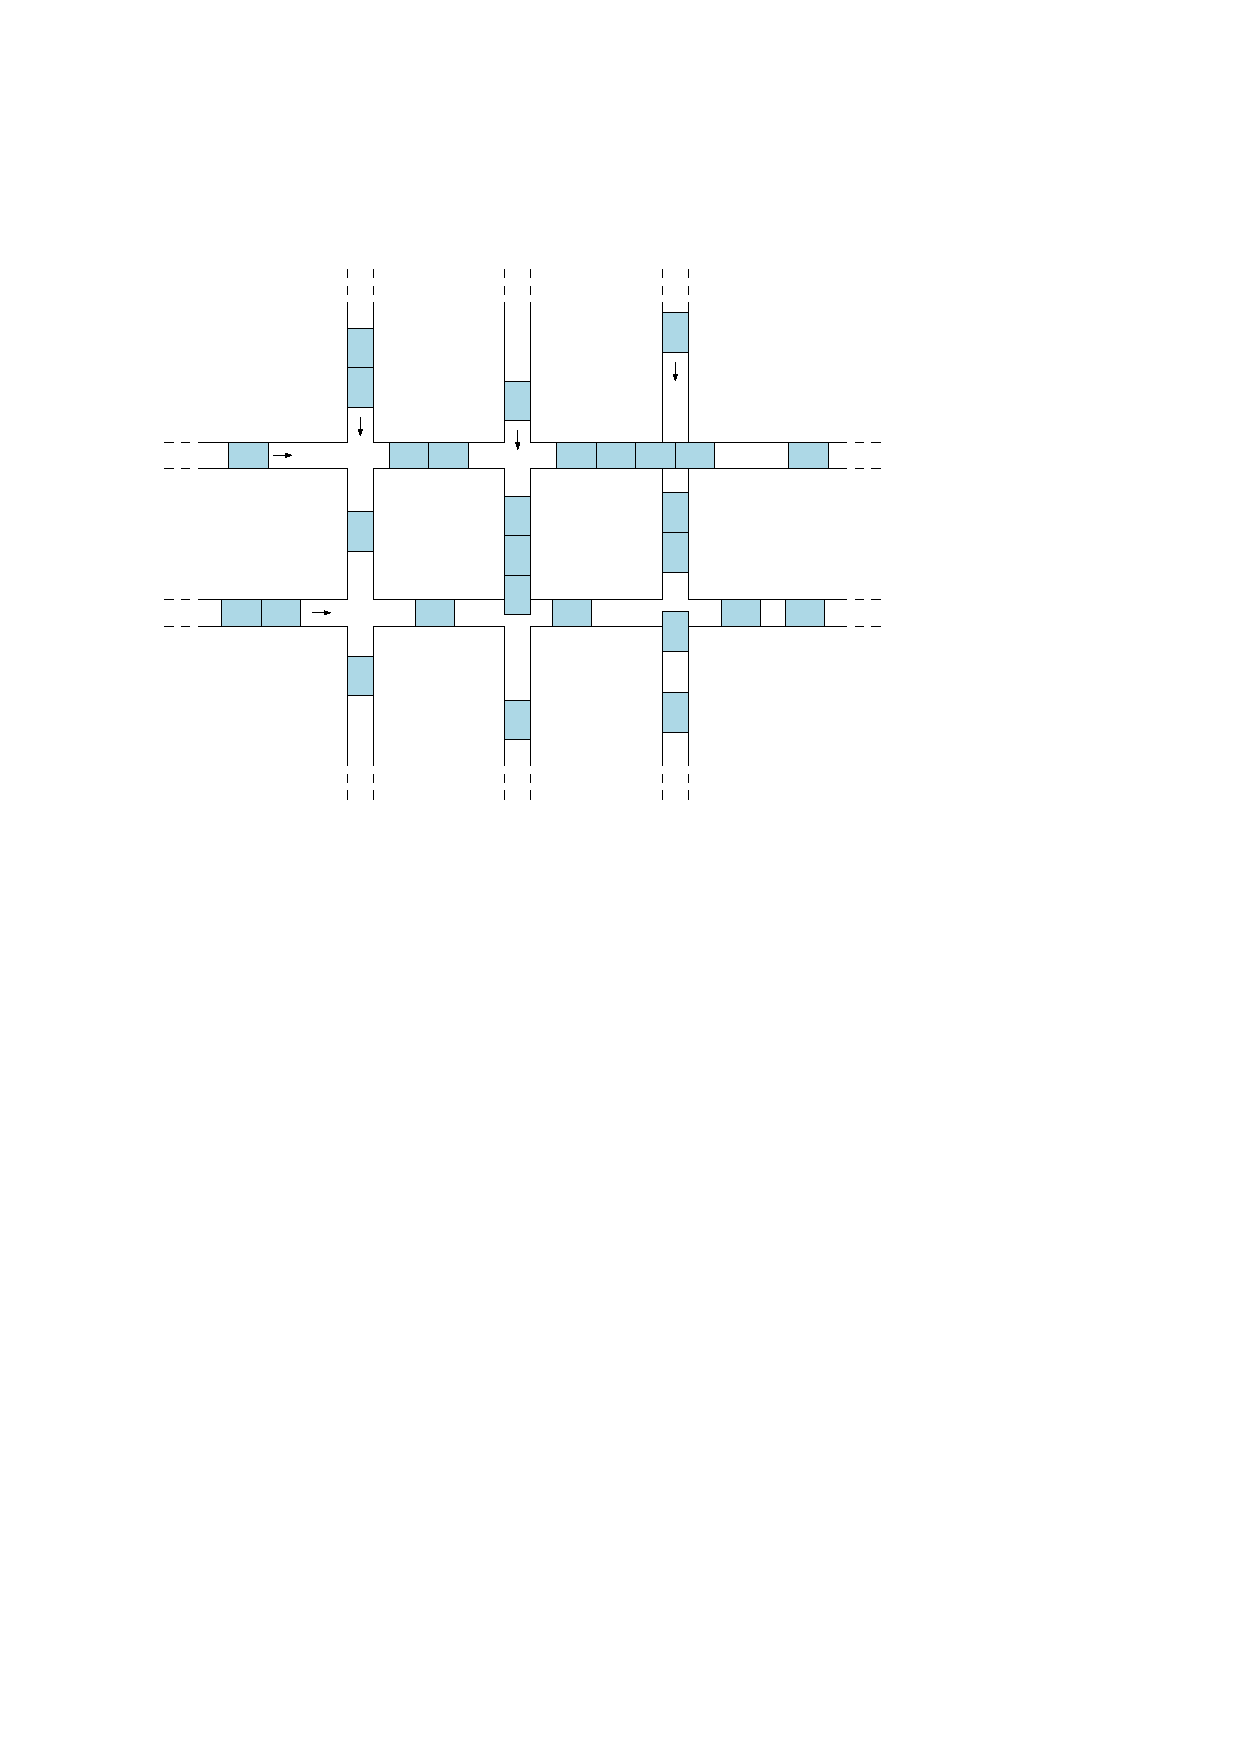
\includegraphics[scale=1]{figures/network-intersections}}
% \microtypesetup{activate}
% \addcontentsline{toc}{part}{Part II \;--\; Networks of Intersections}

% pagebreak in toc listing
\addtocontents{toc}{\protect\newpage}

\chapter{Networks of intersections}\label{chap:network-learning}

We now turn to extending the methodology of the previous chapters to networks.
With some mild assumptions on the paths that vehicles take through the network,
much of what we have done so far extends to networks of intersections.

\paragraph{Network model.}
First, we introduce some graph notation to model simple networks of
intersections with fixed routes. To keep it simple, we assume that routes are
independent, in the sense that vehicles of different routes only meet at
intersection; there is no merging and splitting of routes.
%
We will see that the trajectory optimization problem~\eqref{eq:T} considered so
far extends immediately to this model.

\paragraph{Decomposition.}

It is possible to solve the resulting network trajectory problem using direct
transcription. However, we will now demonstrate this. Instead, we show how the
bilevel decomposition extends to networks. Similar to what we did
in~\Cref{sec:delay-minimization}, we will again assume that the objective only
involves delay and that vehicles are required to cross intersections at full
speed.
%
In this case, however, delay can be measured in two ways: at every intersection,
or at the last intesection of the vehicle's route.

We argue that---in principle---these assumption can be used to reduce the
problem to a scheduling problem. However, compared to the single intersection
setting, there is one additional complicating factor. Before, we did not have to
take into account the maximum number of vehicles that an approaching lane can
handle. However, in the current setting, we can no longer ignore the finite
nature of the lanes between intersection, so they have a \emph{finite capacity}
for vehicles.
%
The precise relationship between the length of the lane and the maximum
acceleration and speed of vehicles turned out to be nontrivial.
%
In other words, it is not easy to characterize the feasibility of trajectories
as a simple set of linear inequalities, like we did for the single intersection,
see~\eqref{eq:feasibility-inequalities}.
%
Our preliminary investigation towards a similar characterization are outlined
in~\Cref{chap:capacitated-lanes}.

\paragraph{Constructive scheduling.}

Instead of a precise characterization of feasibility, we will work with some sufficient conditions.
%
This results in a scheduling problem that is somewhat similar to the classical
job shop scheduling problem.
%
Again, we aim to solve this problem using a constructive heuristic. Quite a few
existing works have adopted the same strategy and applied deep reinforcement
learning successfully.
%
Hence, we mention some pointers for further research to leverage the recent
advances in this field to solve our particular job shop variant.

We identify an issue with the constructive approach. Scheduling decisions
involve picking both an intersection and a route. However, we will see that the
order in which intersections are chosen does not matter for the final schedule.
This redundancy makes the convergence of procedures like policy-gradient very
slow. Removing this redundancy is an interesting direction for further research.

\section{Trajectory optimization in the network model}

\begin{figure}
  \centering
  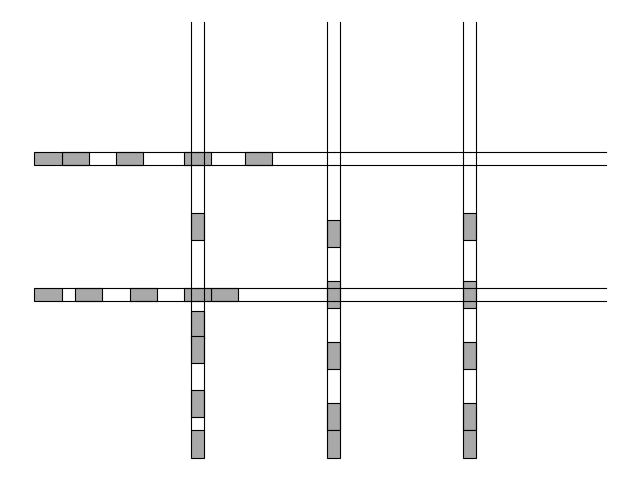
\includegraphics[width=0.55\textwidth]{figures/network/grid_example.png}
  \caption{Illustration of some grid-like network of intersections with vehicles
    drawn as grey rectangles. There are five vehicle routes: two from east to
    west and three from south to north. Turning at intersections is not
    allowed.}\label{fig:network_illustration}
\end{figure}

We now extend the single intersection model to a simple network of intersections
with single lanes where turning is not allowed, illustrated in
Figure~\ref{fig:network_illustration}.

% network definition
\paragraph{Connectivity graph.}
We define a directed graph $(\bar{V},A)$ with nodes $\bar{V}$ and arcs $A$,
representing the possible paths that vehicles can follow. Nodes with only
outgoing arcs are \textit{entrypoints} and nodes with only incoming arcs are \textit{exitpoints}.
Let $V$ be the set of \textit{intersections}, which are all the nodes with
in-degree at least two.
%
Let $d(v, w)$ denote the distance between nodes $v$ and $w$.
%
For each route index $r \in \mathcal{R}$, we let
\begin{align*}
  \bar{V}_{r} = (v_{r}(0), v_{r}(1), \dots, v_{r}(m_{r}), v_{r}(m_{r}+1))
\end{align*}
be the path that vehicles on this route follow through the network. We require
that the first node $v_{r}(0)$ is an entrypoint and that the last node
$v_{r}(m_{r}+1)$ is an exitpoint and we write
\begin{align*}
  V_{r} = \bar{V}_{r} \setminus \{ v_{r}(0), \, v_{r}(m_{r}+1) \}
\end{align*}
to denote the path restricted to intersections. We say that some $(v, w) \in A$
is on path $V_{r}$ whenever $v$ and $w$ are two consecutive nodes on the path
and we write $A_{r}$ to denote the set of all these arcs. We require that
routes can only overlap at nodes by making the following assumption.

\begin{assump}\label{assump:disjoint-routes}
  For every distinct routes $p,q \in \mathcal{R}$ such that $p \neq q$, we
  assume $A_{p} \neq A_{q}$.
\end{assump}

\paragraph{Conflicting positions.}
We start by considering networks in which all roads are axis-aligned, such that
intersections always involve perpendicular lanes and where routes are such that
no turning is required. For each $k\in \{1, \dots, m_r\}$, we define the conflict zone
$\mathcal{E}_{rk} = (B_{rk}, E_{rk} + L)$ and define the union
\begin{align*}
  \mathcal{E}_{r} = \bigcup_{k=1}^{m_r} \mathcal{E}_{rk}
\end{align*}
corresponding to the positions of vehicles for which it occupies an intersection
on its path $V_{r}$, see also Figure~\ref{fig:intersections}.
%
By setting $\mathcal{E}_r \equiv \mathcal{E}$, the single intersection problem
naturally extends to the network case.
%
We will also write $\mathcal{E}_r(v) := \mathcal{E}_{rk}$ with $k$ such that
$v_r(k) = v$ to denote the positions of vehicles from route $r$ that occupy
intersection $v$.

\paragraph{Vehicle indices.}
Again, we will write $\mathcal{N}$ to denote all the vehicles in the system and
$\mathcal{N}_r$ to denote vehicles on route $r \in \mathcal{R}$.
%
Assumption~\ref{assump:disjoint-routes} ensures that the relative ordering of
vehicles on each route is completely determined by their initial positions.
Hence, we write $\mathcal{C}$ for all consecutive pairs of vehicles and
$\mathcal{C}_r$ for a specific route.
%
Collisions can now occur at multiple intersections, so we define
\begin{align}
  \label{eq:6}
  \mathcal{D}^v := \{ \{i, j\} \subset \mathcal{N} : r(i) \neq r(j) , v\in V_{r(i)} \cap V_{r(j)}\}  ,
\end{align}
which are pairs of vehicles that have conflicting paths at some intersection
$v \in V$.

\begin{figure}
  \centering
  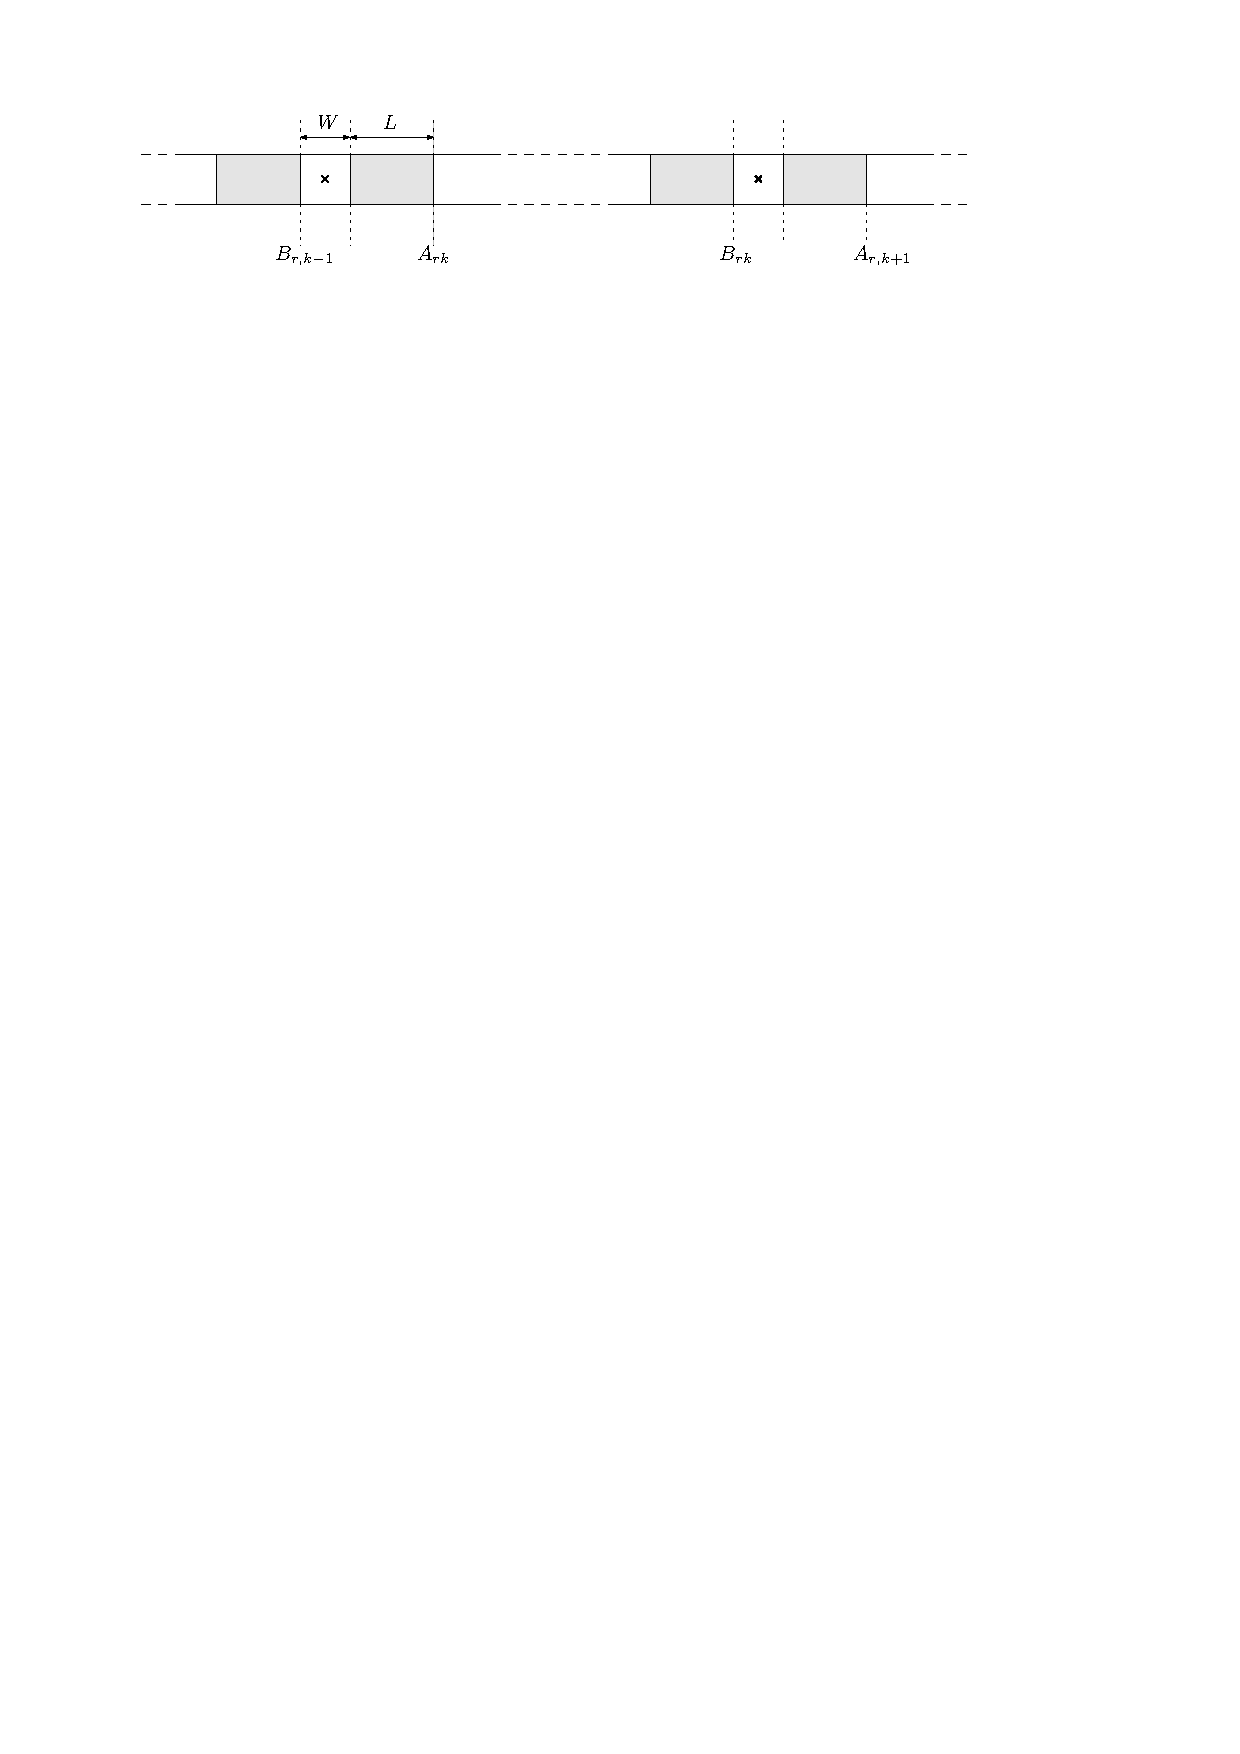
\includegraphics[scale=1]{figures/motion/intersection}
  \caption{Illustration of a route with intersections, marked with a little
    cross. The length of each intersection is $W$. The four shaded rectangles
    illustrate four possible vehicle positions. The conflict areas
    $\mathcal{E}_{rk} = (B_{rk}, E_{rk} + L)$ indicated the positions of the front
    of the vehicle that correspond to occupying some intersection.}%
  \label{fig:intersections}
\end{figure}

\paragraph{Trajectory optimization problem.}

The single intersection trajectory optimization problem~\eqref{eq:T} immediately
extends to the network case.
%
Let $s = \{ s_i = (x_i^0, v_i^0) : i \in \mathcal{N} \}$ denote the initial
state of all vehicles in the system. We consider the same vehicle dynamics as in
the single intersection model, written as $x_i \in D(s_i)$.
%
Let $J(x_i)$ be some trajectory performance criterion. Assume that the network
$(V,A)$ is given and the system parameters
$(L, \mathcal{E}_r, \bar{v}, \omega, \bar{\omega}, t_f)$ are fixed, with $t_f$
some final time and let $x := \{ x_i : i \in \mathcal{N} \}$ denote the joint
position of all vehicles. Consider the following optimization problem over $x$.
%
\begin{alignat}{3}\label{eq:N}
  J(s) := \min_x & \sum_{i \in \mathcal{N}} J(x_i) \tag{NT} \\
      \text{s.t. }&  x_i \in D(s_i) && \quad \text{ for all } i \in \mathcal{N} , \tag{NT.1} \\
                       &  x_i(t) - x_j(t) \geq L && \quad \text{ for all } (i,j) \in \mathcal{C} , \tag{NT.2} \\
                       &  (x_i(t), x_j(t)) \notin \mathcal{E}_{r(i)} \times \mathcal{E}_{r(j)} && \quad \text{ for all } \{i,j\} \in \mathcal{D}^v \text{ and  } v \in V . \tag{NT.3}
\end{alignat}
%
Like before, the resulting problem can be numerically solved by a direct
transcription method.
%
However, this does not scale to networks of practically relevant sizes, so we
will immediately turn our attention to decomposing and reducing the problem into
a more manageable formulation.

\subsection{Bilevel decomposition}

The decomposition for the single intersection extends to the
network model as follows. Let for each pair $(i,v)$ of some vehicle
$i \in \mathcal{N}$ and an intersection $v \in V_{r(i)}$ along its route, let
\begin{align*}
y(i, v) := \inf \{ t: x_{i}(t) \in \mathcal{E}_{r}(v) \} \;\; \text{ and } \;\;  z(i, v) := \sup \{ t: x_{i}(t) \in \mathcal{E}_{r}(v) \}
\end{align*}
be the crossing time and exit time, respectively. We also define $\sigma(i, v) = z(i, v) - y(i, v)$, which
is the amount of time vehicle $i$ occupies intersection $v$.
%
Let $(\mathrm{NT}')$ denote the problem~\eqref{eq:N} with the additional
requirement that $y(i,v) < \infty$ and $z(i, v) < \infty$ for all
$i \in \mathcal{N}$ and $v \in V_r$, then we claim that $(\mathrm{NT}')$ is
equivalent to solving the upper-level occupancy time slot scheduling problem
\begin{alignat}{3}
  U(s) := \min_{y,z} \;\; & \sum_{r \in \mathcal{R}} F(y_{r}, z_{r}, s_r) \tag{NU} \\
  \text{ s.t. } & y(i,v) + \sigma(i,v) \leq y(j,v) \text{ or } \notag \\
                & y(j,v) + \sigma(j,v) \leq y(i,v) , && \quad \text{ for all } \{i,j\} \in \mathcal{D}^{v} \text{ and } v \in V, \tag{NU.1} \\
  & (y_{r}, z_{r}) \in \mathcal{S}_{r}(s_r) , &&  \quad \text{ for all } r \in \mathcal{R} , \tag{NU.2}
\end{alignat}
%
where $F(y_{r}, z_{r}, s_r)$ and $\mathcal{S}_{r}$ are the value function and
set of feasible parameters, respectively, of the parametric lower-level
trajectory optimization problems
%
\begin{alignat}{3}
  F(y_{r}, z_{r}, s_r) = \min_{x_{r}} & \; \sum_{i \in \mathcal{N}_{r}} J(x_{i}) \tag{NL} \\
  \text{ s.t. } & x_{i}(t) \in D_{i}(s_{i}) , && \quad \text{ for } i \in \mathcal{N}_{r} , \tag{NL.1} \\
  & x_{i}(t) - x_{j}(t) \geq L , && \quad \text{ for } (i, j) \in \mathcal{C} \cap \mathcal{N}^2_{r} , \tag{NL.2} \\
  & x_{i}(y(i,v)) = B_{r}(v) , && \quad \text{ for } v \in V_{r} \text{ and } i \in \mathcal{N}_{r} , \tag{NL.3} \\
  & x_{i}(z(i,v)) = E_{r}(v) + L , && \quad \text{ for } v \in V_{r} \text{ and } i \in \mathcal{N}_{r} , \tag{NL.4}
\end{alignat}
where we use subscript $r$ to group variables according to their associated route.
%
A rigorous proof of this fact would be a trivial extension of the proof
presented for Theorem~\ref{thm:decomposition} and does not provide further
insight.

\subsection{Isolating the occupancy scheduling problem}

We make the following assumptions, similar to~\Cref{sec:delay-minimization}.

\begin{assump}[Full speed]
  Each vehicle starts at full speed $v_i^0 = \bar{v}$ and must enter each
  intersection $v \in \mathcal{V}_{r(i)}$ along its path at full speed.
\end{assump}

\begin{define}[Earliest crossing time]
  Consider some vehicle $i$ on route $r = r(i)$. For some trajectory $x_i$ and
  initial state $s_i = (x_i^0, \bar{v})$, define the \emph{earliest crossing
    time} of vehicle $i$ at intersection $v \in V_{r}$ to be
  $a(i, v) := (B_{r}(v) - x_i^0) / \bar{v}$.
\end{define}

\begin{assump}[Uniform intersection]
  We assume that all intersection areas are of the same length, so
  $E_{rk} - B_{rk} = E_{r'k'} - B_{r'k'}$, for all $r, r'$ and $k,k'$. Suppose
  some vehicle drives at full speed as long as it occupies an intersection. In
  that case, the vehicle occupies the intersection for a duration of precisely
  $\sigma := (E_{rk} + L - B_{rk}) / \bar{V}$, with arbitary $r$ and $k$. Again,
  define the \emph{processing time} $\rho := L / \bar{v}$ and let
  $\delta := \sigma - \rho$ denote the \emph{switch-over time}.
\end{assump}

\begin{define}[Delay criteria]
  Consider the total delay a vehicle experiences along its entire trip through
  the network, which we define to be
  $J_d(x_i) = y(i, v_r(m_r)) - a(i, v_r(m_r))$. Alternatively, we could take
  into account the sum of delay experienced at each intersection, given by
  $J'_{d}(x_i) = \sum_{v \in V_{r(i)}} y(i, v) - a(i, v)$.
\end{define}

Using the same reasoning as in~\Cref{sec:delay-minimization}, the full speed
crossing assumption causes the feasibility of the lower-level problems to depend
only on $y$.
This means that we have $z(i, v) = y(i, v) + \sigma$.
%
Let
$ y_r := \{ y(i, v) : i \in \mathcal{N}, v \in V_{r} \}$,
then we can focus on
\begin{align}
  \mathcal{Y}(s_r) := \{ y_r : (y_r, y_r + \sigma) \in \mathcal{S}(s_r)  \} .
\end{align}
%
Furthermore, it can be shown that each lower-level trajectory optimization
problem for a given route $r \in \mathcal{R}$ decomposes into a sequence of
problems, each corresponding to two consecutive intersection along $V_{r}$.
%
This means that $y_{r} \in \mathcal{Y}_{r}$ is essentially equivalent to
$y_{(v,w)} \in \mathcal{Y}_{(v,w)}$ for each $(v,w) \in A_{r}$, where
$y_{(v,w)}$ denotes the vector of all variables $y(i, v)$ and $y(i, w)$ for all
$i \in \mathcal{N}_{r}$ and $\mathcal{Y}_{(v,w)}$ denotes the set of values of
$y_{(v,w)}$ for which a feasible trajectory part can be found.
%
Like we mentioned in~\Cref{sec:delay-minimization}, it is non-trivial to
formulate a polyhedral characterization of $\mathcal{Y}_{(v,w)}$.
%
Without rigorous proof, we now provide some sufficient conditions:

\begin{subnumcases}{y_r \in \mathcal{Y}(s_r) \iff }
        a(i, v) \leq y(i, v) & for $i \in \mathcal{N}_r$  and $v \in V_r$,  \\
        y(i, v) + \rho \leq y(j, v) & for $(i, j) \in \mathcal{C} , v \in V_{r(i)=r(j)}$,  \\
        y(i, v) + d(v,w) / \bar{v} \leq y(i, w) & for $i \in \mathcal{N} , (v,w) \in A_{r(i)}$, \label{travel}  \\
        y(i + c(v,w), w) \leq y(i, v)  & for $i \in \mathcal{N}, (v, w) \in A_r$, \label{buffer}
\end{subnumcases}
where $c(v, w)$ denotes the \emph{capacity} of the lane between intersections
$v$ and $w$, being the maximum number of vehicles for which there is room on
this lane.
%
We refer to~\eqref{travel} as the \emph{travel constraint}, since it encodes the
minimum time necessary for some vehicle $i$ to travel from node $v$ to the next
$w$.
%
We refer to~\eqref{buffer} as the \emph{buffer constraint}, because it
essentially says that there must be room in the lane $(v,w)$ before vehicle $i$
can enter.
%
In general, we conjecture that this constraint can be relaxed slightly. Our
preliminary investigation of this issue is presented in the next chapter.

\section{Network scheduling}

The discussion above guides us in formulating the extension of the crossing time scheduling problem~\eqref{eq:C} to networks of intersections.
Consider the following scheduling problem.
\begin{alignat}{3}
  \min_{y} & \sum_{i \in \mathcal{N}} \sum_{v \in V_{r(i)}} y(i, v) \tag{NC} \label{NC} \\
  \text{ s.t. } & a(i, v) \leq y(i, v) && \text{ for all } i \in \mathcal{N}, v \in V_{r(i)} , \tag{NC.1}\label{eq:travel} \\
                & y(i, v) + \rho \leq y(j, v) && \text{ for all } (i, j) \in \mathcal{C}, v \in V_{r(i)=r(j)} , \tag{NC.2} \\
                & y(i,v) + \sigma(i,v) \leq y(j,v) \text{ or } \quad \notag \\
                & y(j,v) + \sigma(j,v) \leq y(i,v) , && \text{ for all } \{i,j\} \in \mathcal{D}^{v} \text{ and } v \in V, \tag{NC.3} \label{eq:network-disj} \\
                & y(i, v) + d(v,w) / \bar{v} \leq y(i, w) && \text{ for } i \in \mathcal{N} , (v,w) \in A_{r(i)}, \tag{NC.4} \label{eq:travel} \\
                & y(i + c(v,w), w) \leq y(i, v) && \text{ for  } i \in \mathcal{N}, (v,w ) \in A_{r(i)} . \tag{NC.5} \label{eq:buffer}
\end{alignat}

After encoding the constraints~\eqref{eq:network-disj} with binary variables and
the big-$M$ trick, we can again reformulate this problem as a mixed-integer
linear program.

\subsection{Constructive scheduling}

Without going into detail, we will now discuss some of our preliminary findings
with respect to extending the constructive scheduling approach
of~\Cref{chap:single-learning}.
%
Instead of a single vehicle and route order, we must now deal with a separate
vehicle order $\nu^v$ and route order $\eta^v$ for each intersection $v \in V$.
%
The constructive scheduling MDP must be extended accordingly. This means that
each state is  of the form
\begin{align}
  s_t := (\omega, \{ \eta^v : v \in V \})
\end{align}
where an instance is given by $\omega = (a, \rho, \sigma)$ with $a := \{ a(i,v) \}$ denoting all
earliest arrival times.
%
Consequently, each action now corresponds to selecting a route-intersection pair
$(r, v)$, causing $r$ to be appended to the route order $\eta^v$.

Furthermore, the analysis of~\Cref{sec:sequence-representation} can be extended, by considering the disjunctive graph over nodes $(i, v)$ and encoding the constraints of~\eqref{NC}.
%
Note that we now have a new type of conjunctive arc $(i, v)  \rightarrow (i, w)$
with weight $d(v,w) /\bar{v}$ due to the constraints~\eqref{eq:travel}, and conjunctive arc
$(i + c(v,w), w) \rightarrow (i, v)$ with weight $0$ due to the
constraints~\eqref{eq:buffer}.
%
Again, it can be shown that optimal schedules need to
satisfy~\eqref{eq:active_schedule}, where $\mathcal{N}^-$ now involves these
additional arcs. Furthermore, the definition of crossing time lower bounds
naturally extends to $\beta_{iv}(s_t)$, for each vehicle-intersection pair
$(i, v)$.

\subsection{Learning to schedule}

We will now briefly discuss some of our preliminary findings on extending the
methodology of~\Cref{chap:single-learning} to networks.

\paragraph{Intersection visit order.}

In the general class of sequence models, of which our MDP model is a special
case (we are essentially learning a sequence of actions), it has been noted
before that the order in which inputs or outputs are presented to the model
during training has a considerable impact on the final model
fit~\cite{vinyalsOrderMattersSequence2016}.
%
For our model, we also expect to find this effect, so we investigated the impact
of the order in which intersections are visited.
% random
First of all, the simple \textit{random} strategy would be to sample some
intersection with pending crossings at each step.
% ``boundary'' (or ``exhaustive'')
In the \textit{boundary} strategy, we keep visiting the same intersection until
it is done (when it has no pending crossings anymore), then move to some next
intersection. When the network of intersections is free of cycles, we could for
example follow some topological order. We use the term ``boundary'' because this
strategy produces trajectories along the boundary of the grid in
Figure~\ref{fig:solution_equivalence}.
% ``alternate''
In the \textit{alternating} strategy, we keep alternating between intersection
to keep the number of scheduled vehicles balanced among them. This produces
trajectories that can be understood as being close to the ``diagonal'' of the
grid in Figure~\ref{fig:solution_equivalence}.

\begin{figure}
  \centering
  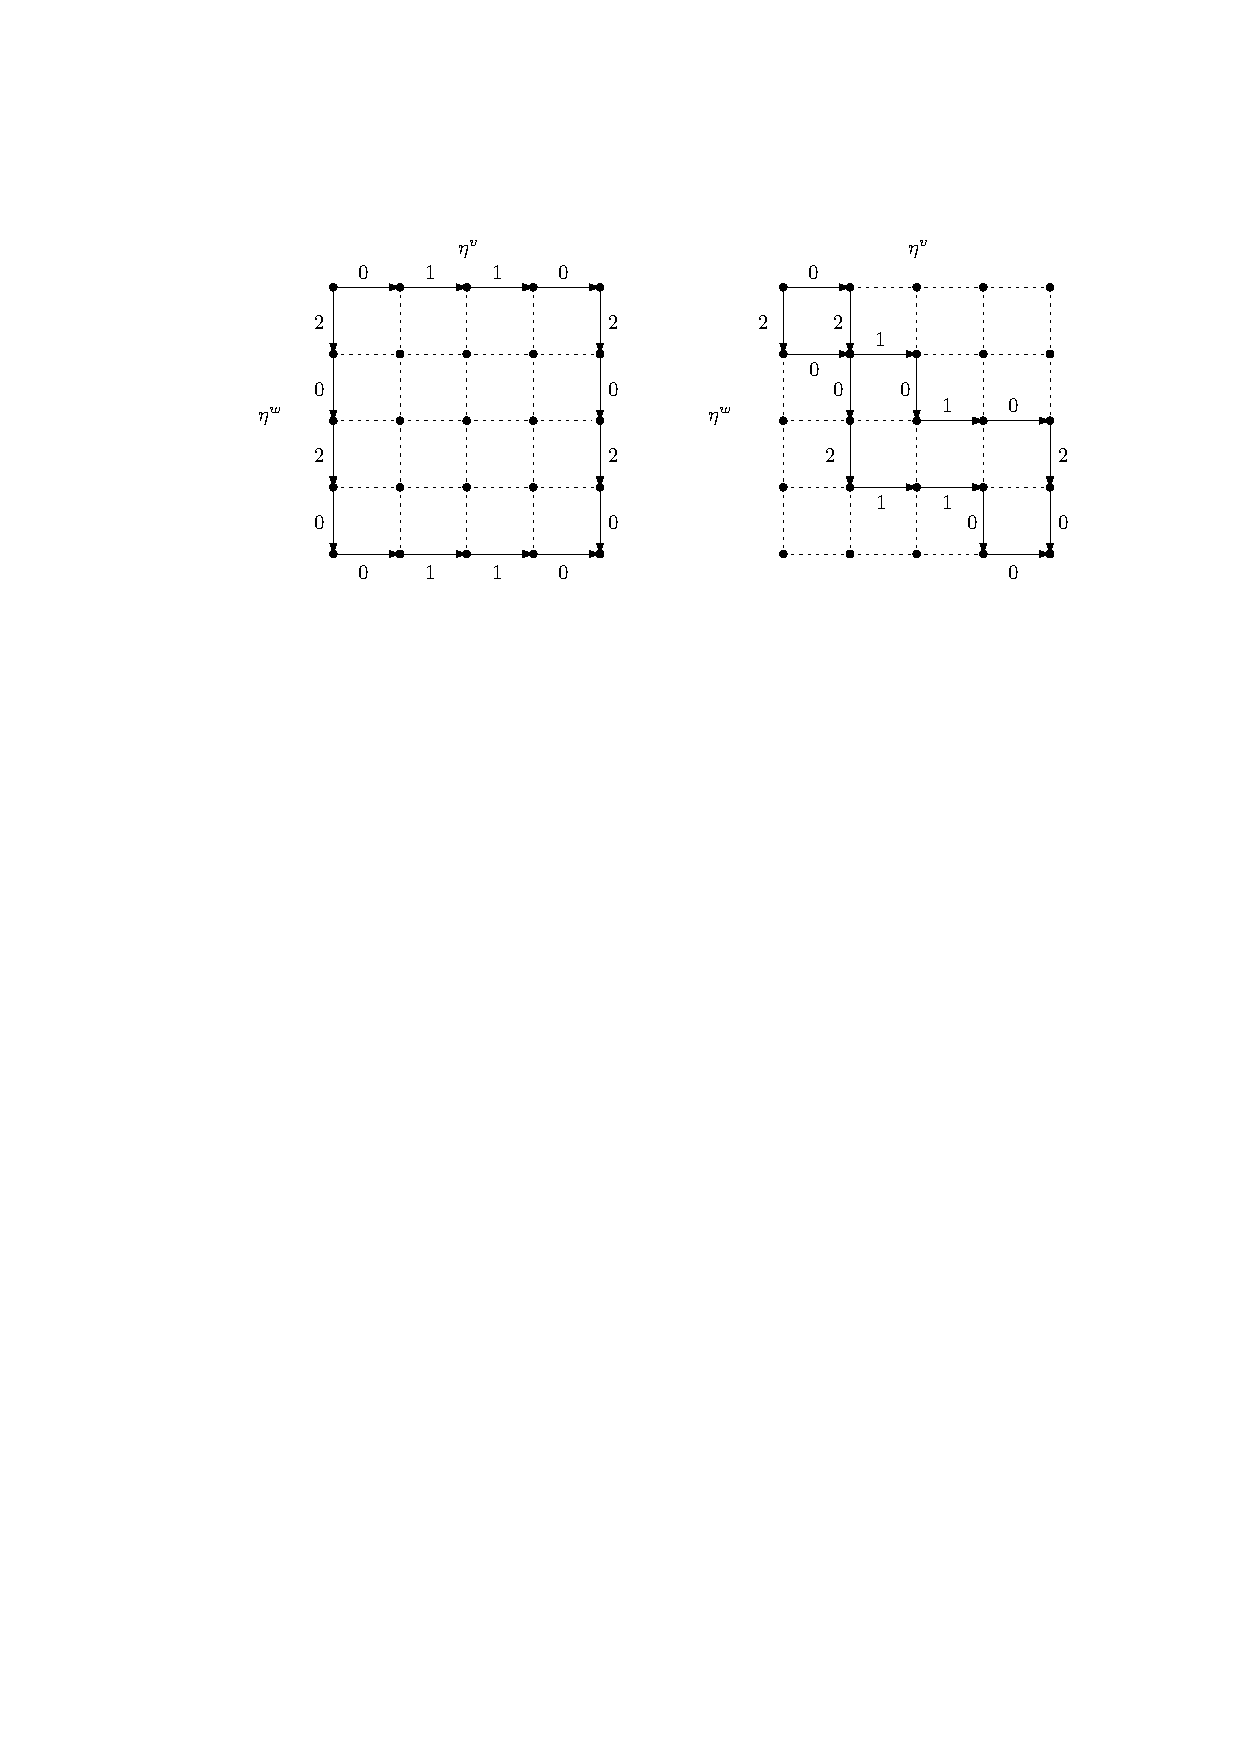
\includegraphics[width=0.9\textwidth]{figures/network/solution_equivalence}
  \caption{When each route order is locally fixed at every intersection, the
    global crossing sequence is not uniquely determined, because these local
    sequences may be merged in any order. Suppose we have a tandem of two
    intersections and a horizontal arrows correspond to taking the next local
    action at intersection $v$, a vertical arrows correspond to taking next
    local action at intersection $w$. Each valid crossing sequence corresponds
    to some path from the top-left to the bottom-right corner. Although any such
    crossing sequence produces the same schedule, it might be that our
    model fits better on some sequences than others. For example,
    we might expect that sequences on the boundary of the grid, shown in the
    left grid, are harder to learn from data than sequences that stay closer to
    the diagonal, like in the right grid. The intuition is that we need to
    ``look into the future'' more to learn the former, while in the latter
    trajectories, progress in the two intersections is more balanced.}
  \label{fig:solution_equivalence}
\end{figure}

\paragraph{Threshold heuristics.}
It is straightforward to extend the threshold rule to networks of
intersections, when assuming a fixed intersection order. Each time some
next intersection is visited, we apply the single intersection threshold rule to
pick the next route. This is straightforward to do, because we can just consider
the disjunctive subgraph induced by the nodes belonging to that intersection to
arrive at the single intersection case.
%
Furthermore, the definition of the threshold rule itself does not depend on the
network of intersections. This is a desirable property, because it allows us to
tune the threshold on small networks and then apply it on larger ones.

\paragraph{Neural constructive heuristic.}

The neural network parameterization of~\eqref{sec:neural-param} can be extended
to networks.
%
The model can be best understood as solving a multi-label classification
problem, because it needs to provide a distribution over routes at every
intersection.
%
Under the imitation learning regime, the training data set $\mathcal{X}$
consists of state-action pairs $(s_{t-1}, (r_{t}, v_{t}))$.
%
To obtain these pairs, we again sample a collection of problem instances, which
are solved to optimality using a MILP solver, and for each optimal schedule, we
backtrack the corresponding optimal route order $\eta^{v}$ for each
intersection.

From these optimal route orders, we can construct $\mathcal{X}$ in different
ways, depending on the specific intersection visit order that is used.
% multiple intersection order per instance
The model might become more robust when training on multiple samples of
intersections orders per instance.
% fixed intersection order
Alternatively, we can consider one of the fixed intersection orders
described at the start of this section (random, boundary, alternating).

% silent package loading


\begin{knitrout}
\definecolor{shadecolor}{rgb}{0.969, 0.969, 0.969}\color{fgcolor}\begin{table}
\centering
\caption{\label{tab:results}Average scaled optimal objective value computed using MILP and using the threshold heuristic with threshold $\tau = 0$. Each class of problem instances is identified by the number $n$ of vehicle arrivals per route and the grid network size as cols x rows.}
\centering
\resizebox{\ifdim\width>\linewidth\linewidth\else\width\fi}{!}{
\begin{tabular}[t]{cc|cc|c|c|c|ccc|cc|c|c|c|ccc|cc|c|c|c|ccc|cc|c|c|c|ccc|cc|c|c|c|ccc|cc|c|c|c|ccc|cc|c|c|c|ccc|cc|c|c|c|c}
\toprule
n & size & MILP & time & $\tau = 0$  (gap) & random (gap) & boundary (gap) & alternate (gap)\\
\midrule
5 & 2x1 & 57.27 & 0.06 & 65.27 (11.45\%) & 58.96 (2.95\%) & 58.72 (2.52\%) & 58.23 (1.66\%)\\
5 & 3x1 & 57.67 & 0.12 & 68.34 (15.44\%) & 59.77 (3.65\%) & 59.82 (3.74\%) & 58.72 (1.83\%)\\
5 & 3x2 & 57.35 & 1.38 & 69.17 (18.32\%) & 60.88 (6.16\%) & 60.36 (5.25\%) & 58.82 (2.56\%)\\
\bottomrule
\end{tabular}}
\end{table}

\end{knitrout}



\section{Notes and references}

We emphasize again that the assumption of crossing the intersection at maximum
speed is a central feature of our model, because it causes intersections to act
as a sort of ``checkpoints''.
%
The fact that the global trajectory optimization can be stated as a
jop-shop-like problem hinges on this assumption, because we essentially
``localized'' the effects of the vehicle dynamics to individual lanes; the
coupling between lanes are through the crossing times.
%
In order to relax this assumption and deal with objectives that takes into
account energy or fuel consumption, we need to take make a global trade-off
between fast crossing and energy efficiency, for which more advanced
optimization schemes are required.

Although our network examples are all grid-like and have perpendicular
intersecting lanes, the model proposed in this chapter is more generally
applicable.
%
For example, curved roads can be modeled as well, as long we assume that this
does not affect the dynamics of the vehicles, in particular the maximum speed.

\chapter{Capacitated lanes}\label{chap:capacitated-lanes}


In our presentation of the isolated intersection model, we relied heavily on the
assumption that the intial distance to the intersection was large enough for
each vehicle to allow feasible trajectories.
%
Once we extend our model to the multi-intersection situation, it does no longer
make sense to ignore the finite length of roads between intersections. In other
words, we need to start taking into account the \emph{finite capacity} for
vehicles of each lane between intersections.
%
In order to formulate a model for a network of intersections, we formulate
and analyze a model for such a \emph{capacitated lane}.

We will propose a model for a one-directional single-lane road of finite length
where overtaking is not permitted.
%
The fact that such a lane can be occupied by a limited number of vehicles at the
same time, makes the characterization of set of feasible trajectories more
involved.
%
% feasibility analysis (of safe sets of trajectories)
Given some lane, consider the set of vehicles that need to travel across this
lane as part of their planned route. Suppose that the time of entry to and exit
from this lane are fixed for each of these vehicles, then the question is
whether there exists a set of trajectories that is safe, i.e., without
collisions, and which satisfies these \emph{schedule times}.
%
Loosely speaking, we ask whether there exists an easy way to answer this
feasibility question for any set of schedule times.
%
By requiring vehicles to enter and exit the lane at \emph{full speed}, we will
conjecture that the answer positive, in the sense that the feasibility question
is precisely answered by a system of linear inequalities in terms of the
schedule times.

\section{Model formulation}

We start by establishing the notion of a feasible set of trajectories
in the capacitated lane.

\paragraph{Vehicle trajectories.}
We only consider the longitudinal position of vehicles on the lane and we assume
that speed and acceleration are bounded. Therefore, let $\mathcal{D}[a,b]$
denote the set of valid \emph{trajectories}, which we define to be all continuously
differentiable functions $x : [a,b] \rightarrow \mathbb{R}$ satisfying the constraints
\begin{align}
  \dot{x}(t) \in [0, 1] \quad \text{ and } \quad
  \ddot{x}(t) \in [{-\omega} ,\bar{\omega}] , \quad \text{ for all } t \in [a,b] ,
\end{align}
for some fixed acceleration bounds $\omega, \bar{\omega} > 0$ and with $\dot{x}$ and
$\ddot{x}$ denoting the first and second derivative with respect to time $t$.
Note that the unit speed upper bound is not restrictive, since we can always
apply an appropriate scaling of time and the acceleration bounds to arrive at
this form.
%
We use $A$ and $B$ to denote the start\footnote{Note that assuming $A\neq 0$ is convenient later when we start piecing together multiple lanes.} and end position of the lane.
%
Let $D_{1}[a, b] \subset \mathcal{D}[a, b]$ denote all trajectories $x$ that satisfy
the first-order boundary conditions
\begin{align}
  x(a) = A \; \text{ and } \; x(b) = B
\end{align}
and additionally satisfy $\dot{x}(a) > 0$ and $\dot{x}(b) > 0$, to avoid the
technical difficulties of dealing with vehicles that are waiting at the start or
end of the lane.
%
On top of these conditions, let $D_{2}[a,b] \subset D_{1}[a, b]$ further induce the
second-order boundary conditions
\begin{align}
  \dot{x}(a) = \dot{x}(b) = 1 .
\end{align}
In words, these boundary conditions require that a vehicle arrives to and
departs from the lane at predetermined times $a$ and $b$ and do so at full
speed.
%
Figure~\ref{fig:trajectories} shows an example for each of these three classes of trajectories.

\begin{figure}
  \centering
  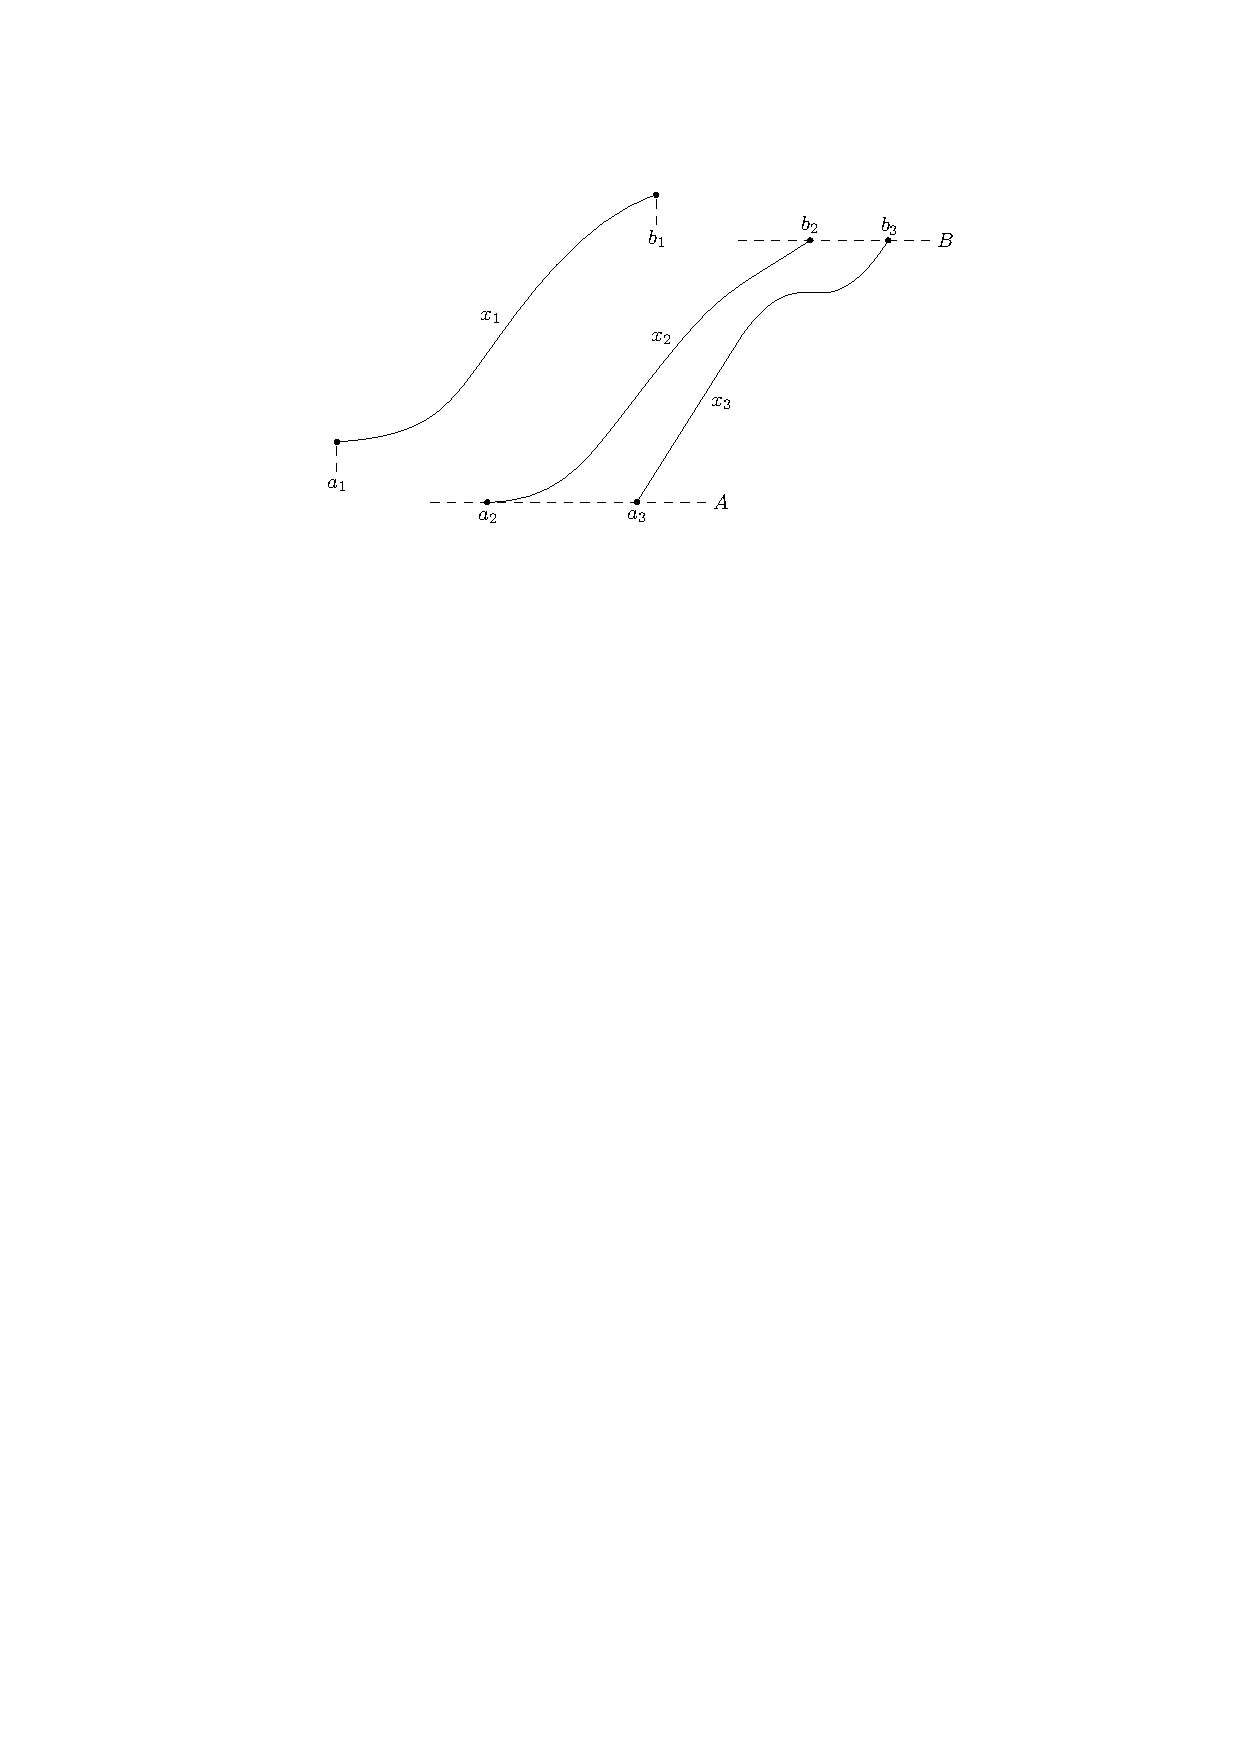
\includegraphics[scale=0.9]{figures/motion/trajectories}
  \caption{Example trajectories $x_{1} \in \mathcal{D}[a_{1},b_{1}]$,
    $x_{2} \in D_{1}[a_{2},b_{2}]$ and $x_{3} \in D_{2}[a_{3},b_{3}]$ for each
    the three classes of trajectories that are used throughout this chapter
    (horizontal axis is time, vertical axis is position).}%
  \label{fig:trajectories}
\end{figure}

\paragraph{Trajectory domains.}
Function domains will play an important role in the analysis of feasible
trajectories. Therefore, we introduce some useful notational conventions.
%
First of all, each of the trajectory classes above can be used with the common
convention of allowing $a = -\infty$ or $b = \infty$. For instance, we write
$\mathcal{D}(-\infty, \infty)$ to denote the set of trajectories defined on the
whole real line.
%
Furthermore, we use $\cdot\,|_{[a,b]}$ to denote function restriction. For example,
\begin{align*}
  (t \mapsto t + 1)|_{\halfopen{\xi}{\infty}}
\end{align*}
denotes some anonymous function with some restricted domain.
%
Furthermore, given two smooth trajectories $\gamma_{1} \in \mathcal{D}[a_{1}, b_{1}]$
and $\gamma_{2} \in \mathcal{D}[a_{2}, b_{2}]$, we write inequality
  $\gamma_{1} \preceq \gamma_{2}$ to mean
\begin{align*}
\gamma_{1}(t) \leq \gamma_{2}(t) \; \text{ for all } \; t \in [a_{1}, b_{1}] \cap [a_{2}, b_{2}] .
\end{align*}
%
Whenever the intersection of domains is empty, we say that the above inequality
is \emph{void}.
%
The reason for introducing a dedicated symbol is that $\preceq$ is not transitive.
To see this, consider the trajectories in Figure~\ref{fig:trajectories}, then
$x_{1} \preceq x_{3}$ (void) and $x_{3} \preceq x_{2}$, but clearly
$x_{1} \npreceq x_{2}$.

\begin{define}
  Let $L > 0$ denote the \textit{following distance} between consecutive vehicles.
  %
  Suppose there are $N$ vehicles scheduled to traverse the lane. For each
  vehicle $i$, let $a_{i}$ and $b_{i}$ denote the \textit{schedule time} for entry and
  exit, respectively.
  %
  Assuming that the schedule times are ordered as
  $a_{1} \leq a_{2} \leq \dots \leq a_{N}$ and
  $b_{1} \leq b_{2} \leq \dots \leq b_{N} $, then a \emph{feasible solution} consists
  of a sequence of trajectories $x_{1}, \dots, x_{N}$ such that
\begin{subequations}\label{eq:feasibility}
\begin{align}
x_{i} \in D_{2}[a_{i}, b_{i}] \quad \quad & \text{ for each } i \in \{1, \dots, N\}, \label{eq:second-order-constraint} \\
x_{i} \preceq x_{i-1} - L \quad \quad & \text{ for each } i \in \{2, \dots, N\} . \label{eq:lead-constraint}
\end{align}
\end{subequations}
We will refer to~\eqref{eq:lead-constraint} as the \emph{lead vehicle
  constraints}.
%
For some performance criterion of trajectories, given as a functional $J(x)$ of
trajectory $x$, the \emph{lane planning problem} is to find a feasible solution that
maximizes
\begin{align}\label{eq:objective}
  \min \; \sum_{i=1}^{N} J(x_{i}) .
\end{align}
\end{define}

We emphasize again that~\eqref{eq:second-order-constraint} requires vehicles to
enter and exit the lane at full speed.
%
The feasibility characterization that we will derive can now be roughly stated
as follows. Assuming the system parameters $(\omega, \bar{\omega},A,B,L)$ to be
fixed, with lane length $B-A$ sufficiently large and following distance $L$
sufficiently small, feasibility of the lane planning problem is characterized by
a system of linear inequalities in terms of the schedule times $a_{i}$ and
$b_{i}$.

% \subsection{Direct transcription}

% A straightforward way of solving
% problem~\eqref{eq:feasibility}--\eqref{eq:objective} is through direct
% transcription to a mixed-integer linear program by only considering the vehicle
% trajectories $x_{i}(t)$ at discrete time steps $t_{1}, t_{2}, \dots, t_{n}$.
% %
% We can use the forward Euler scheme to discretize the constraints.
% %
% The downside of this technique is that its computational complexity scales very
% poorly with the number of time steps.

\section{Single vehicle with arbitrary lead vehicle constraint}\label{sec:single-vehicle-problem}

Before we analyze the feasibility of the lane planning problem as a whole, we
focus on the lead vehicle constraint~\eqref{eq:lead-constraint} for a single
vehicle $i \geq 2$.
%
This allows us to lighten the notation slightly by dropping the vehicle index
$i$. Instead of $x_{i-1} - L$, we assume we are given some arbitrary \emph{lead vehicle boundary}
$u$ and consider the following problem.

\begin{define}
  Let $u \in D_{1}[c, d]$ and assume we are given two schedule times
  $a,b \in \mathbb{R}$, then the \emph{single vehicle (feasibility) problem} is to find
  a trajectory $x \in D_{2}[a,b]$ such that $x \preceq u$.
\end{define}

\subsection{Necessary conditions}

Suppose we are given some feasible trajectory $x$ for the single vehicle
problem.
%
In addition to the given upper bounding trajectory $u$, we will derive two
upper bounding trajectories $x^{1}$ and $\hat{x}$ and one lower bounding
trajectory $\check{x}$, see Figure~\ref{fig:necessary-conditions}.
%
Using these bounding trajectories, we will formulate four necessary conditions
for the single vehicle problem.

Let the \emph{full speed boundary}, denoted $x^{1}$, be defined as
\begin{align}
  x^{1}(t) = A + t - a,
\end{align}
for all $t \in [a, b]$, then we clearly have $x \preceq x^{1}$. Observe that
$x^{1}(s) = B$ for $s = a + (B-A)$, which can be interpreted as the earliest
time of departure from the lane, so we must have $b \geq a + (B-A)$. This is our
first necessary condition.
%
\begin{lemma}\label{lemma:travel-constraint}
  If there exists $x\in D_{2}[a,b]$, then $b-a \geq B-A$.
\end{lemma}

Next, since deceleration is at most $\omega$, we have
$\dot{x}(t) \geq \dot{x}(a) - \omega(t - a) = 1 - \omega(t - a)$, which we
combine with the speed constraint $\dot{x} \geq 0$ to derive
$\dot{x}(t) \geq \max\{0, 1 - \omega (t - a) \}$. Hence, we obtain the lower
bound
\begin{align}\label{eq:check-x}
  x(t) = x(a) + \int_{a}^{t} \dot{x}(\tau) \diff \tau \geq A + \int_{a}^{t} \max\{0, 1 - \omega (\tau - a) \} \diff \tau =: \check{x}(t) ,
\end{align}
for all $t \geq a$, so that we have $x \succeq \check{x}$.
%
Analogously, we derive an upper bound from the fact that acceleration is at most $\bar{\omega}$. Observe that we have
$\dot{x}(t) + \bar{\omega} (b - t) \geq \dot{x}(b) = 1$, which we combine
with the speed constraint $\dot{x}(t) \geq 0$ to derive
$\dot{x}(t) \geq \max \{ 0, 1 - \bar{\omega}(b - t) \}$. Hence, we obtain the
upper bound
\begin{align}\label{eq:hat-x}
  x(t) = x(b) - \int_{t}^{b} \dot{x}(\tau) \diff \tau
  \leq B - \int_{t}^{b} \max\{ 0, 1 -\bar{\omega} (b - \tau) \} \diff \tau =: \hat{x}(t) ,
\end{align}
for all $t \leq b$, so we have $x \preceq \hat{x}$.
%
We refer to $\check{x}$ and $\hat{x}$ as the \emph{entry boundary} and
\emph{exit boundary}, respectively.

\begin{figure}
  \centering
  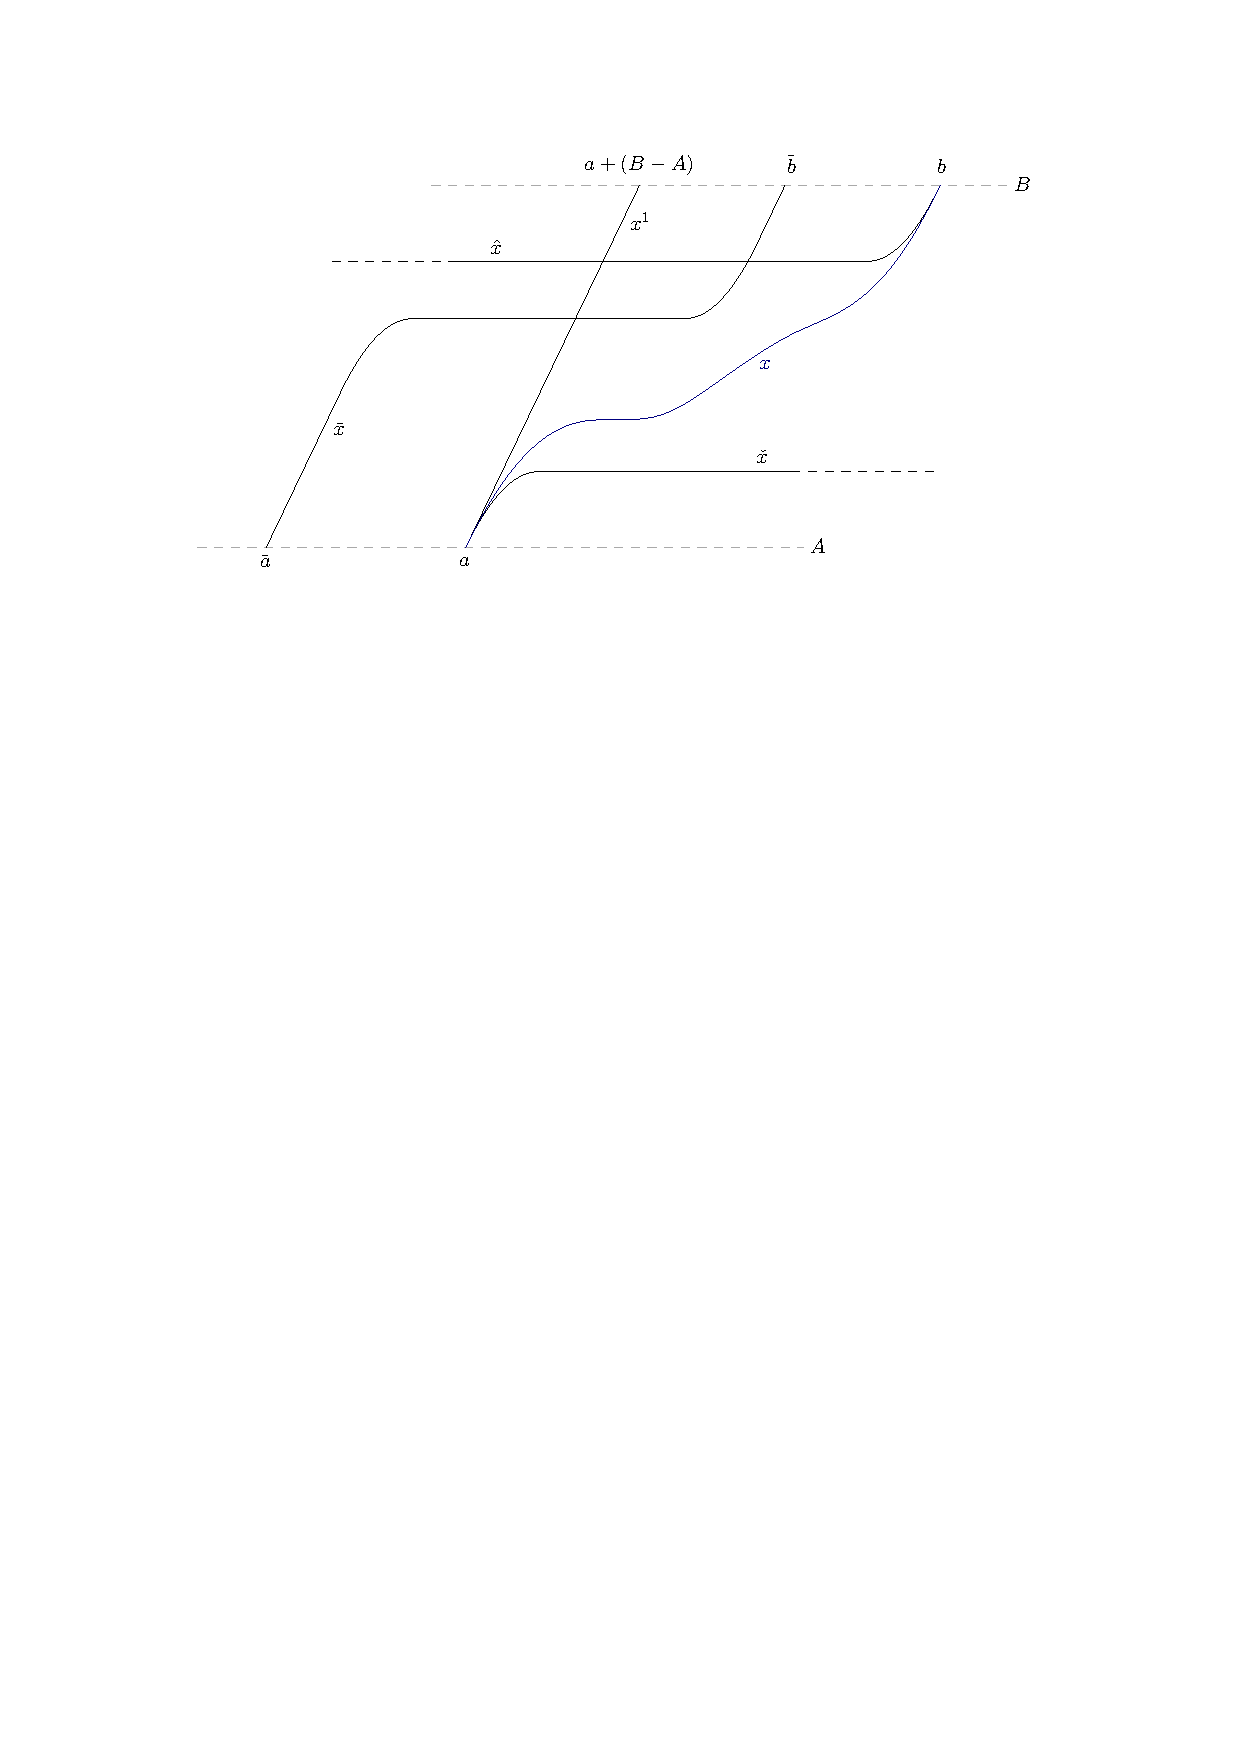
\includegraphics[scale=0.9]{figures/motion/necessary-conditions}
  \caption{Illustration of the four bounding trajectories
    $u, x^{1}, \hat{x}, \check{x}$ that bound feasible trajectories from
    above and below. We also drew an example of a feasible trajectory $x$ in
    blue. The horizontal axis represents time and the vertical axis corresponds
    to the position on the lane, so the vertical dashed grey lines correspond to
    the start and end of the lane.}%
  \label{fig:necessary-conditions}
\end{figure}

\begin{lemma}\label{lemma:necessary-conditions}
  Consider some lead boundary $u \in D_{1}[c,d]$ and assume
  $[a,b] \cap [c,d] \neq \varnothing$. If there exists a trajectory
  $x \in D_{2}[a, b]$ such that $x \preceq u$, then $a \geq c$ and $b \geq d$ and $u \succeq \check{x}$.
  % \begin{itemize}[leftmargin=3em,midpenalty=5]
  %   \item $a \geq c$,
  %   \item $b \geq d$,
  %   \item $u \succeq \check{x}$.
  % \end{itemize}
\end{lemma}
\pagebreak[1]
\begin{proof}
  Each of these conditions corresponds somehow to one of the bounding
  trajectories defined above.
  %
  Suppose $a < c$, then because the domains intersect, we must have $b > c$, but
  then clearly no $x$ can satisfy $x \preceq u$.
  %
  When $b < d$, then it is a consequence of $\dot{u}(b) > 0$ that any $x$ will
  violate $x \preceq u$.
  %
  To see that the third condition must hold, suppose that $u(\tau) < \check{x}(\tau)$
  for some time $\tau$. Since $c \leq a$, this means that $u$ must intersect
  $\check{a}$ from above. Therefore, any trajectory that satisfies $x \preceq u$
  must also intersect $\check{a}$ from above, which contradicts the assumption
  $x \in D_{2}[a,b]$.
\end{proof}

\begin{remark}
  The assumption of non-empty domains is required in the previous lemma, because
  otherwise we include the situation in which $x$ lies completely to the left of
  $u$, in which case the stated conditions are obviously not necessary anymore.
\end{remark}

We note that the boundaries $\hat{x}$ and $\check{x}$ can be combined to
yield yet another necessary condition.
%
It is straightforward to verify from~\cref{eq:hat-x,eq:check-x} that
$\hat{x}(t) \geq B - 1/(2\bar{\omega})$ and $\check{x}(t) \leq A + 1/(2\omega)$.
%
Therefore, whenever $B - A < 1/(2\bar{\omega}) + 1/(2\omega)$, these boundaries intersect
for certain values of $a$ and $b$.
%
Because the exact condition is somewhat cumbersome to characterize, we avoid
this case by simply assuming that the lane length is sufficiently large, to keep
the analysis simpler.

\begin{assump}\label{assump:lane-length}
  The length of the lane satisfies $B - A \geq 1/(2\omega) + 1/(2\bar{\omega})$.
\end{assump}

Observe that $1/(2\omega)$ is precisely the distance required to decelerate from
full speed to a standstill. Similarly, $1/(2\bar{\omega})$ is the distance
required for a full acceleration. Therefore, we may interpret
Assumption~\ref{assump:lane-length} as requiring enough space in the lane such
that there is at least one \emph{waiting position}.
%
We will return to this observation in
Section~\ref{sec:lane-problem-feasibility}.
\note{(check that we do this)}


\subsection{Sufficient conditions}\label{sec:optimal-trajectory}

\begin{figure}
  \centering
  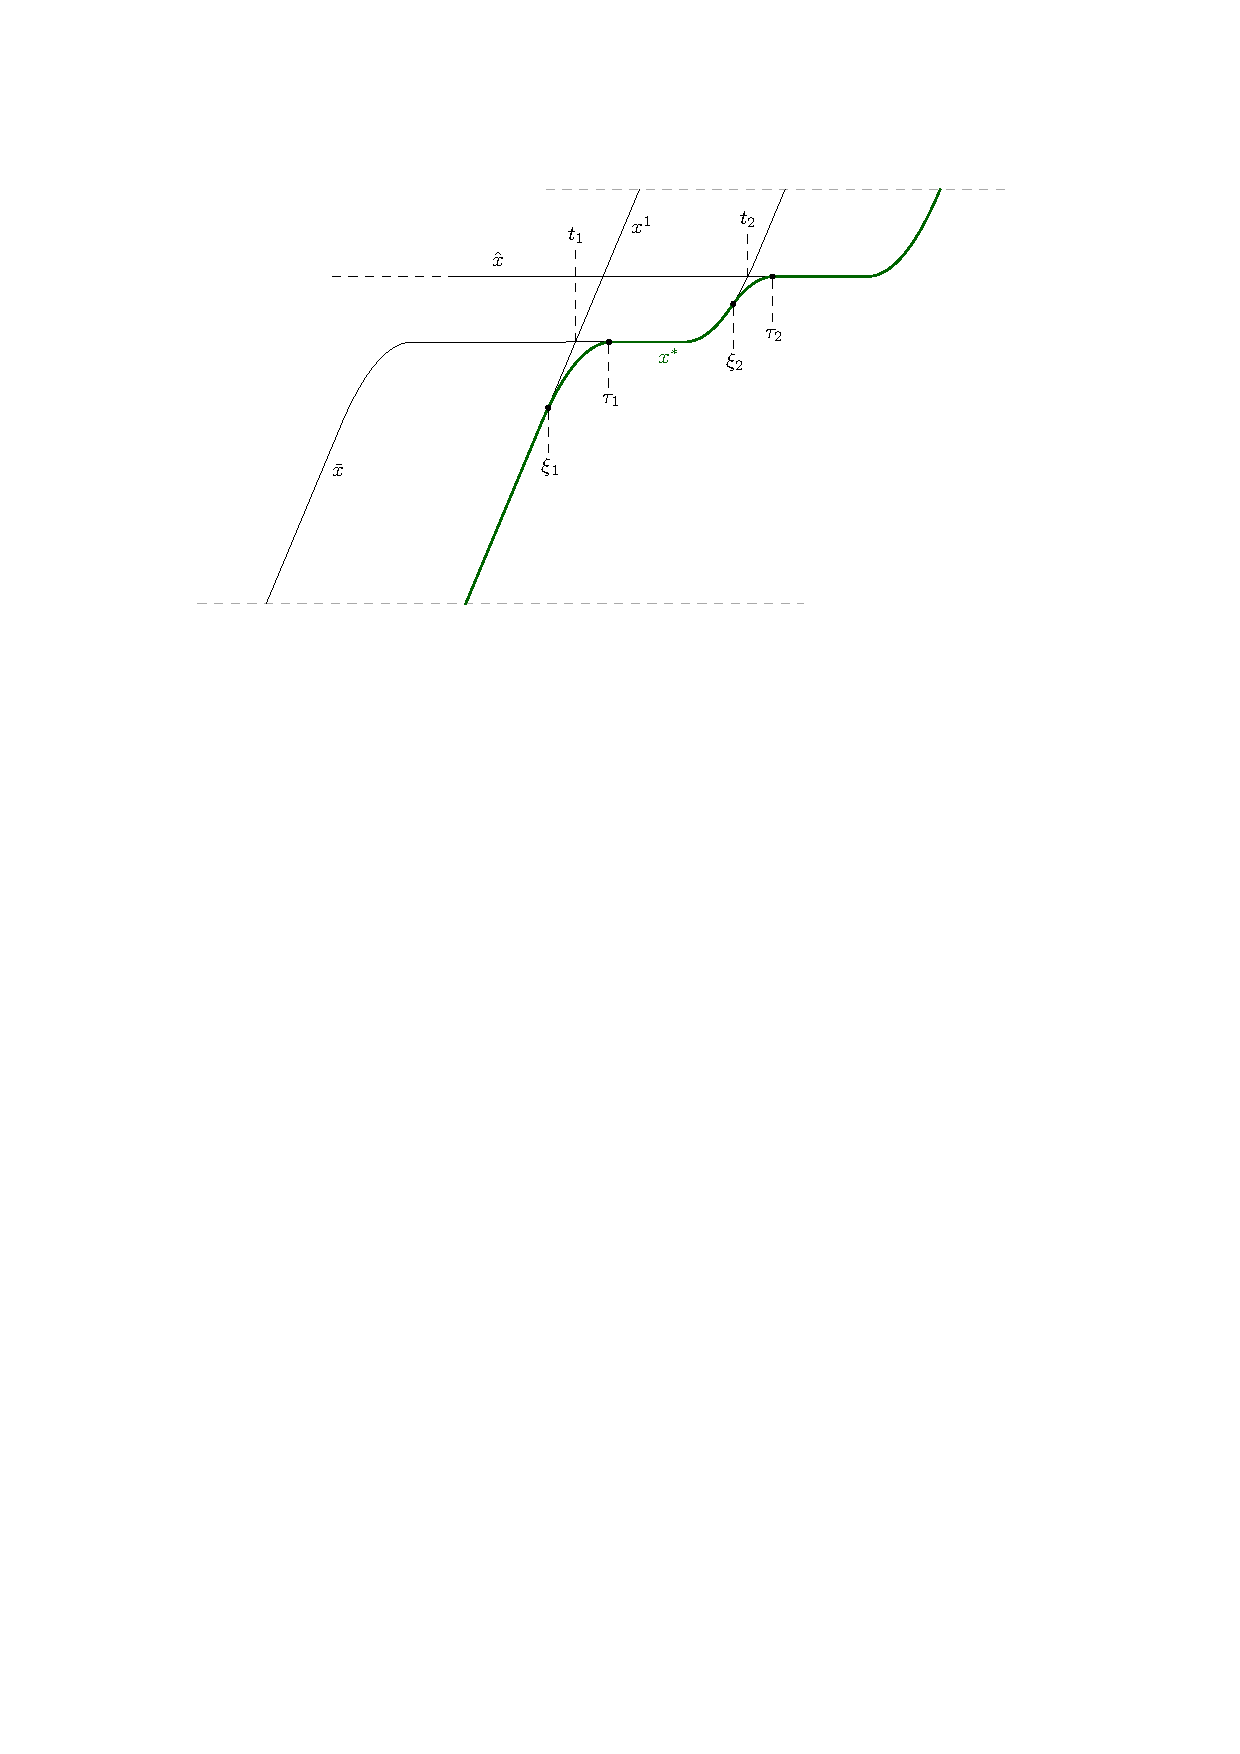
\includegraphics[scale=1]{figures/motion/proof}
  \caption{The minimum boundary $\gamma$, induced by three upper boundaries
    $u$, $\hat{x}$ and $x^{1}$, is smoothened around time $t_{1}$ and
    $t_{2}$, where the derivative is discontinuous, to obtain the smooth optimal
    trajectory $x^{*}$, drawn in green. The times $\xi_{i}$ and $\tau_{i}$
    correspond to the start and end of the connecting deceleration as
    defined in Section~\ref{sec:smoothing}.}%
  \label{fig:optimal-construction}
\end{figure}

The goal of the remainder of this section is to prove the following feasibility
characterization.

\begin{theorem}[Feasibility characterization of single vehicle
  problem]\label{thm:single-vehicle}
  Given some lead vehicle boundary $u \in D_{1}[c,d]$ and some schedule times
  $a, b \in \mathbb{R}$ such that $[a,b]\cap [c,d] \neq \varnothing$ and assuming
  Assumption~\ref{assump:lane-length}, there exists a solution
  $x \in D_{2}[a,b]$ satisfying $x \preceq u$ if and only if \TabPositions{3cm}
  \begin{enumerate}[label=(\roman*)\quad,leftmargin=5em,midpenalty=5]
    \item $b-a \geq B-A$, \tab (travel constraint)
    \item $a \geq c$, \tab (entry order constraint)
    \item $b \geq d$, \tab (exit order constraint)
    \item $u \succeq \check{x}$. \tab (entry space constraint)
  \end{enumerate}
\end{theorem}

Note that Lemma~\ref{lemma:travel-constraint} and Lemma~\ref{lemma:necessary-conditions} already showed
necessity of these conditions.
%
Therefore, we will show that, under these conditions, we can always construct a
solution $\gamma^{*}$ for the single vehicle problem, thereby showing that the
four conditions are also sufficient.
%
The particular solution that we will construct also happens to be a smooth upper
boundary for all other solutions, in the sense that, for any other feasible
solution $x$ we have $x \preceq \gamma^{*}$.
%
The starting point of the construction is the \emph{minimum boundary}
$\gamma : [a,b] \rightarrow \mathbb{R}$, defined as
\begin{align}\label{eq:min-boundary}
  \gamma(t) := \min \{ u(t), \hat{x}(t), x^{1}(t) \} .
\end{align}
%
Obviously, $\gamma$ is a valid upper boundary for any other feasible solution,
%
but in general, $\gamma$ may have a discontinuous derivative at some\footnote{In fact, it can be shown that, under the necessary conditions, there are at most two of such discontinuities.} isolated
points in time, in which case $\gamma \notin \mathcal{D}[a,b]$.

\begin{define}\label{def:piecewise-trajectory}
  Let $\mathcal{P}[a,b]$ be the set of functions $\mu : [a, b] \rightarrow \mathbb{R}$ for
  which there is a finite subdivision $a = t_{0} < \cdots < t_{n+1} = b$ such that
  the truncation $\mu|_{[t_{i}, t_{i+1}]} \in \mathcal{D}[t_{i}, t_{i+1}]$ is
  a smooth trajectory, for each $i \in \{0, \dots, n\}$, and for which the one-sided limits of $\dot{\mu}$ satisfy
  \begin{align}
    \dot{\mu}(t_{i}^{-}) := \lim_{t \uparrow t_{i}} \dot{\mu}(t) > \lim_{t \downarrow t_{i}} \dot{\mu}(t) =: \dot{\mu}(t_{i}^{+}) ,
  \end{align}
  for each $i \in \{1, \dots, n\}$. We refer to such $\mu$ as a \emph{piecewise
    trajectory (with downward bends)}.
\end{define}

Under the conditions of Theorem~\ref{thm:single-vehicle}, it is not difficult to
see from Figure~\ref{fig:necessary-conditions} that $\gamma$ satisfies the above definition, so
$\gamma \in \mathcal{P}[a,b]$. In other words, $\gamma$ consists of a number of pieces that
are smooth and satisfy the vehicle dynamics, with possibly some sharp bend
downwards where these pieces come together.
%
Next, we present a simple procedure to smoothen out this kind of discontinuity
by decelerating from the original trajectory somewhat before some $t_{i}$, as
illustrated in Figure~\ref{fig:optimal-construction}. We will argue that this procedure can be repeated as
many times as necessary to smoothen out every discontinuity.


In Section~\ref{sec:deceleration-boundary}, we first define a parameterized
family of functions to model the deceleration part that we introduce for the
smoothing procedure, which is described in Section~\ref{sec:smoothing}.
%
We apply this procedure to $\gamma$ to obtain $\gamma^{*}$, after which it is
relatively straightforward to show that $\gamma^{*}$ is an upper bound for all
other feasible solutions, which is done in
Section~\ref{sec:upper-bound-property}.


\subsection{Deceleration boundary}\label{sec:deceleration-boundary}
% In order to formalize the smoothing procedure, we will first define some
% parameterized family of functions to model the deceleration part that we
% introduce to smooth the original trajectory.
%
Recall the derivation of $\check{x}$ in equation~\eqref{eq:check-x} and the discussion
preceding it, which we will now generalize a bit.
%
Let $x \in \mathcal{D}[a, b]$ be some smooth trajectory, then observe that $\dot{x}(t) \geq \dot{x}(\xi) - \omega(t - \xi)$ for all $t \in [a, b]$.
Combining this with the constraint $\dot{x}(t) \in [0, 1]$, this yields
\begin{align}
  \dot{x}(t) \geq \max\{ 0, \, \min\{1, \, \dot{x}(\xi) - \omega (t - \xi) \}\} =: \{\dot{x}(\xi) - \omega(t-\xi)\}_{[0,1]} ,
\end{align}
where use $\{ \cdot \}_{[0,1]}$ as a shorthand for this clipping operation.
%
Hence, for any $t \in [a,b]$, we obtain the following lower bound
\begin{align}\label{eq:deceleration-boundary}
  x(t) = x(\xi) + \int_{\xi}^{t} \dot{x}(\tau) \diff \tau \geq x(\xi) + \int_{\xi}^{t} \{\dot{x}(\xi) - \omega(\tau - \xi)\}_{[0,1]} \diff \tau =: x[\xi] (t) ,
\end{align}
where we will refer to the right-hand side as the \emph{deceleration boundary} of $x$
at $\xi$.
%
Observe that this definition indeed generalizes the definition of $\check{x}$,
because we have $\check{x}=(x[a])|_{[a,b]}$.

Note that $x[\xi]$ depends on $x$ only through the two real numbers $x(\xi)$ and
$\dot{x}(\xi)$. It will be convenient later to rewrite the right-hand side
of~\eqref{eq:deceleration-boundary} as
\begin{align}\label{eq:def-x-}
  x^{-}[p, v, \xi](t) := p + \int_{\xi}^{t} \{ v - \omega(\tau - \xi) \}_{[0,1]} \diff \tau ,
\end{align}
such that $x[\xi](t) = x^{-}[x(\xi), \dot{x}(\xi), \xi](t)$.
%
We can expand the integral in this expression further by carefully handling the
clipping operation. Observe that the expression within the clipping operation
reaches the bounds $1$ and $0$ for $\delta_{1} := \xi - (1-v)/\omega$ and
$\delta_{0} := \xi + v/\omega$, respectively. Using this notation, a straightforward
calculation shows that
\begin{align}\label{eq:x-}
  x^{-}[p,v,\xi](t) = p +
  \begin{cases}
    {(1 - v)}^{2} / (2\omega) + (t - \xi) & \text{ for } t \leq \delta_{1} , \\
    v(t - \xi) - \omega{(t-\xi)}^{2} /2 & \text{ for } t \in [\delta_{1} , \delta_{0}] , \\
    v^{2}/(2\omega) & \text{ for } t \geq \delta_{0} .
  \end{cases}
\end{align}
%
It is easily verified that the three cases above coincide at
$t \in \{\delta_{1}, \delta_{0}\}$, which justifies the overlaps in the case distinction.
Furthermore, since $x$ and $\dot{x}$ are continuous by assumption, it follows
that $x[\xi](t) = x^{-}[x(\xi), \dot{x}(\xi), \xi](t)$ is continuous as a function of
either of its arguments.\footnote{Even more, it can be shown that $x[\xi](t)$ is continuous as a function of $(\xi, t)$.}
%
Assuming $0 \leq v \leq 1$, it can be verified that for every $t \in \mathbb{R}$, we
have $\ddot{x}^{-}[p,v,\xi](t) \in \{-\omega, 0\}$ and
$\dot{x}^{-}[p,v,\xi](t) \in [0,1]$ due to the clipping operation, so that
$x^{-}[p,v,\xi] \in \mathcal{D}(-\infty,\infty)$.

\begin{figure}
  \centering
  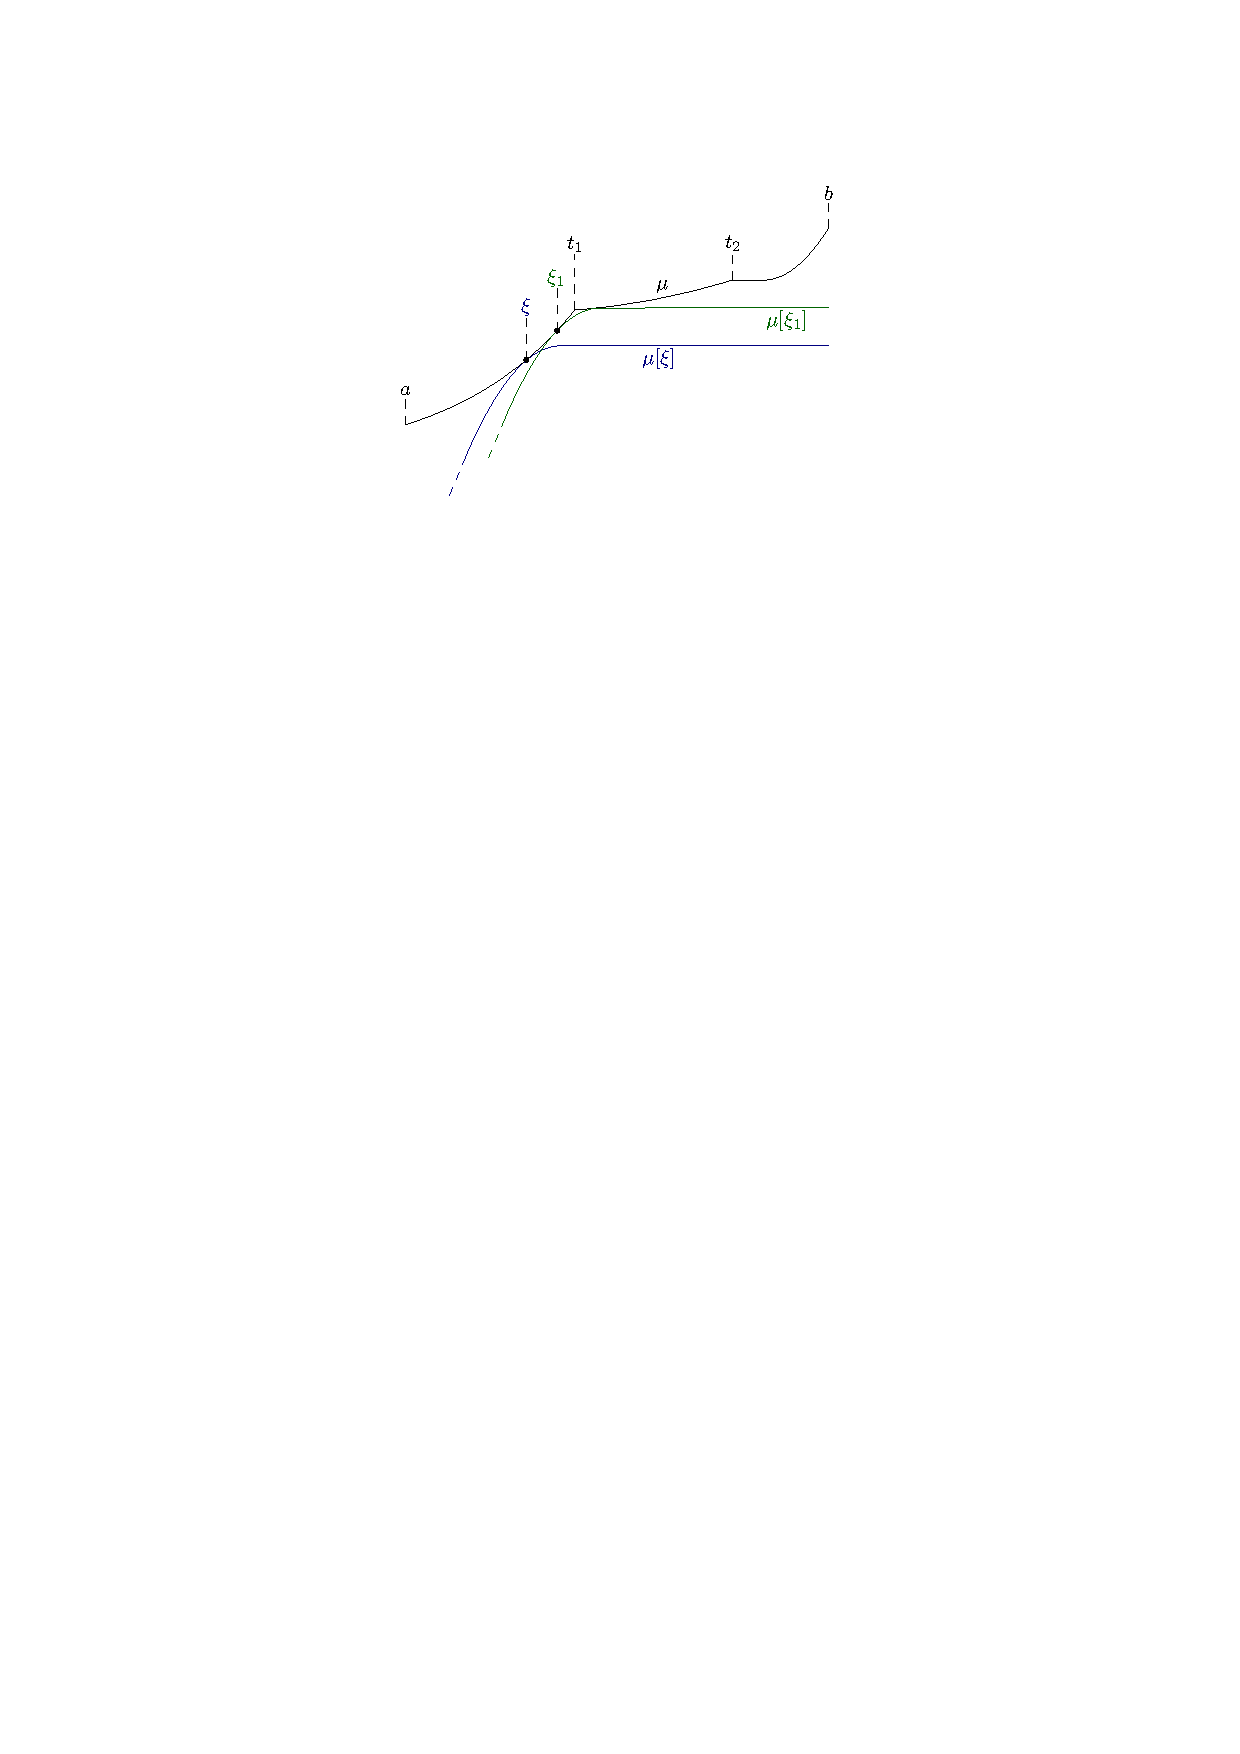
\includegraphics[scale=1.1]{figures/motion/deceleration-boundary}
  \caption{Illustration of some piecewise trajectory $\mu \in \mathcal{P}[a,b]$ with
    a discontinuous derivative at times $t_{1}$ and $t_{2}$. Furthermore, the
    figure shows some arbitrary deceleration boundary $\mu[\xi]$ at time $\xi$ in blue
    and the unique connecting deceleration $\mu[\xi_{1}]$ to the cover discontinuity at
    $t_{1}$ in green. We truncated the start of both deceleration boundaries for
    a more compact figure. The careful observer may notice that $\mu$ cannot occur
    as the minimum boundary defined in~\eqref{eq:min-boundary}, but please note that the class of
    piecewise trajectories $\mathcal{P}[a,b]$ is just slightly more general than
    necessary for our current purposes.}%
  \label{fig:deceleration-boundary}
\end{figure}


\paragraph{Piecewise trajectories.}
Let $\mu \in \mathcal{P}[a, b]$ be some piecewise trajectory with corresponding
subdivision $a = t_{0} < \cdots < t_{n+1} = b$ as defined in Definition~\ref{def:piecewise-trajectory}. It is
straightforward to generalize the definition of a deceleration boundary to $\mu$.
%
Whenever $\xi \in [a,b] \setminus \{ t_{1}, \dots, t_{n}\}$, we just define
$\mu[\xi] := x^{-}[\mu(\xi), \dot{\mu}(\xi), \xi]$, exactly like we did for $x$.
%
However, at the points of discontinuity $\xi \in \{ t_{1}, \dots, t_{n}\}$, the
derivative $\dot{\mu}(\xi)$ is not defined, so we choose to use the left-sided limit
instead, by defining $\mu[\xi] := x^{-}[\mu(\xi), \dot{\mu}(\xi^{-}), \xi]$.

\begin{remarknum}\label{rem:lower-bound-piecewise}
  Please note that we cannot just replace $x$ with $\mu$ in inequality~\eqref{eq:deceleration-boundary} to
  obtain a similar bound for $\mu$ on the its full interval $[a,b]$.
  Instead, we get the following \emph{piecewise lower bounding} property.
  %
  Consider some interval
  $I \in \{ [a, t_{1}], \openhalf{t_{1}}{t_{2}}, \dots, \openhalf{t_{n}}{b} \}$, then what
  remains true is that $\xi \in I$ implies $\mu(t) \geq \mu[\xi](t)$ for every $t \in I$.
\end{remarknum}


\subsection{Smoothing procedure}\label{sec:smoothing}
Let $\mu \in \mathcal{P}[a,b]$ be some piecewise trajectory and let
$a = t_{0} < \cdots < t_{n+1} = b$ denote the subdivision as in Definition~\ref{def:piecewise-trajectory}.
%
We first show how to smoothen the discontinuity at $t_{1}$ and then argue how to
repeat this process for the remaining times $t_{i}$.
Our aim is to choose some time $\xi \in [a,t_{1}]$ from which the vehicle starts
fully decelerating, such that $\mu[\xi] \preceq \mu$ and such that $\mu[\xi]$ touches $\mu$ at some time
$\tau \in [t_{1}, b]$ tangentially.
%
We will show there is a unique trajectory $\mu[\xi]$ that satisfies these requirements
and refer to it as the \emph{connecting deceleration}, see
Figure~\ref{fig:deceleration-boundary} for an example.
%
The construction relies on the following technical assumption.

\begin{assump}\label{assump:smoothing}
  Throughout the following discussion, we assume $\mu \succeq \mu[a]$ and $\mu \succeq \mu[b]$.
\end{assump}



\paragraph{Touching.}
Recall Remark~\ref{rem:lower-bound-piecewise}, which asserts that we have
$\mu[\xi](t) \leq \mu(t)$ for every $t \in [a,t_{1}]$ for any $\xi \in [a, t_{1}]$.
%
After the discontinuity, so for every $t \in [t_{1}, b]$, we want
$\mu[\xi](t) \leq \mu(t)$ and equality at least somewhere, so we measure the relative
position of $\mu[\xi]$ with respect to $\mu$ here, by considering
\begin{align}
  d(\xi) := \min_{t \in [t_{1}, b]} \mu(t) - \mu[\xi](t) .
\end{align}
Since $\mu(t)$ and $\mu[\xi](t)$ are both continuous as a function of $t$ on the interval
$[t_{1}, b]$, this minimum actually exists (extreme value theorem).
%
Furthermore, since $d$ is the minimum of a continuous function over a closed
interval, it is continuous as well (see Lemma~\ref{lemma:inf-continuous}).
%
Observe that $d(a) \geq 0$, because $\mu \succeq \mu[a]$ by Assumption~\ref{assump:smoothing}.
%
By definition of $t_{1}$, we have $\dot{\mu}(t_{1}^{-}) > \dot{\mu}(t_{1}^{+})$,
from which it follows that $\mu(t) < \mu[t_{1}](t)$ for $ t\in (t_{1}, t_{1} + \epsilon)$ for some
small $\epsilon > 0$, which shows that $d(t_{1}) < 0$.
%
By the intermediate value theorem, there is $\xi_{1} \in \halfopen{a}{t_{1}}$ such
that $d(\xi_{1}) = 0$.
%
This shows that $\mu[\xi_{1}]$ touches $\mu$ at some time
$\tau_{1} \in [t_{1}, b]$.


\paragraph{Uniqueness.}
It turns out that $\xi_{1}$ itself is not necessarily unique, which we explain
below. Instead, we are going to show that the connecting deceleration
$\mu[\xi_{1}]$ is unique. More precisely, given any other $\xi \in \halfopen{a}{t_{1}}$ such
that $d(\xi) = 0$, we will show that $\mu[\xi] = \mu[\xi_{1}]$.

The first step is to establish that the level set
\begin{align}
  X := \{ \xi \in \halfopen{a}{t_{1}} : d(\xi) = 0 \}
\end{align}
is a closed interval. To this end, we show that $d$ is non-increasing on
$\halfopen{a}{t_{1}}$, which together with continuity implies the desired result
(see Lemma~\ref{lemma:levelset}).
%
To show that $d$ is non-increasing, it suffices to show that $\mu[\xi](t)$ is
non-decreasing as a function of $\xi$, for every $t \in [t_{1}, b]$.
%
We can do this by computing the partial derivative of $\mu[\xi]$ with respect to $\xi$
and verifying it is non-negativity.
%
Recall the definition of $\mu[\xi]$, based on $x^{-}$ in equation~\eqref{eq:x-}.
%
Using similar notation, we write
$\delta_{1}(\xi) = \xi - (1 - \dot{\mu}(\xi))/\omega$ and
$\delta_{0}(\xi) = \xi + \dot{\mu}(\xi)/\omega$ and compute
%
\begin{align}
  \frac{\partial}{\partial \xi} \mu[\xi](t) =
  \dot{\mu}(\xi) +
  \begin{cases}
    \ddot{\mu}(\xi)(\dot{\mu}(\xi)-1)/\omega - 1 &\text{ for } t \leq \delta_{1}(\xi) , \\
    \ddot{\mu}(\xi)(t-\xi) - \dot{\mu}(\xi) + \omega(t-\xi) &\text{ for } t \in [\delta_{1}(\xi),\delta_{0}(\xi)] , \\
    \ddot{\mu}(\xi)\dot{\mu}(\xi)/ \omega &\text{ for } t \geq \delta_{0}(\xi) .
  \end{cases}
\end{align}
%
It is easily verified that the cases match at
$t \in \{\delta_{1}(\xi), \delta_{0}(\xi)\}$, which justifies the overlaps there.
%
Consider any $\xi \in \halfopen{a}{t_{1}}$ and $t \in [t_{1}, b]$, then we always have
$\delta_{1}(\xi) \leq \xi \leq t$, so we only have to verify the second and third case:
%
\begin{subequations}
\begin{alignat}{2}
  \frac{\partial}{\partial \xi} \mu[\xi](t) &= (\ddot{\mu}(\xi) + \omega)(t-\xi) \geq 0 \quad\quad\quad &&\text{ for } t \in [\delta_{1}(\xi) ,\delta_{0}(\xi)], \label{eq:case2} \\
  \frac{\partial}{\partial \xi} \mu[\xi](t) &\geq \dot{\mu}(\xi) + (-\omega)\dot{\mu}(\xi)/\omega = 0 &&\text{ for } t \geq \delta_{0}(\xi) . \label{eq:case3}
\end{alignat}
\end{subequations}
%
This concludes the argument for $X$ being a closed interval.

Assuming $\xi$ to be fixed, observe that there is equality in~\eqref{eq:case2} for some
$t \in [\delta_{1}(\xi), \delta_{0}(\xi)]$ if and only if there is equality in~\eqref{eq:case3}
for some other $t' \geq \delta_{0}(\xi)$. Note that this happens precisely when
$\ddot{\mu}(\xi) = -\omega$.
%
Therefore, whenever $\mu$ is fully deceleration, so $\dot{\mu}(t)=-\omega$ on
some open interval $U \subset (a, t_{1})$, we have
$(\partial/\partial \xi) \mu[\xi](t) = 0$ for all $t \geq \delta_{1}(\xi)$.
%
This essentially means that any choice of $\xi \in U$ produces the same
trajectory $\mu[\xi]$. Please see Figure~\ref{fig:deceleration-boundary-unique}
for an example of this case.
%
This observation is key to the remaining uniqueness argument.

\begin{figure}[h]
  \centering
  \vspace*{0.5em}
  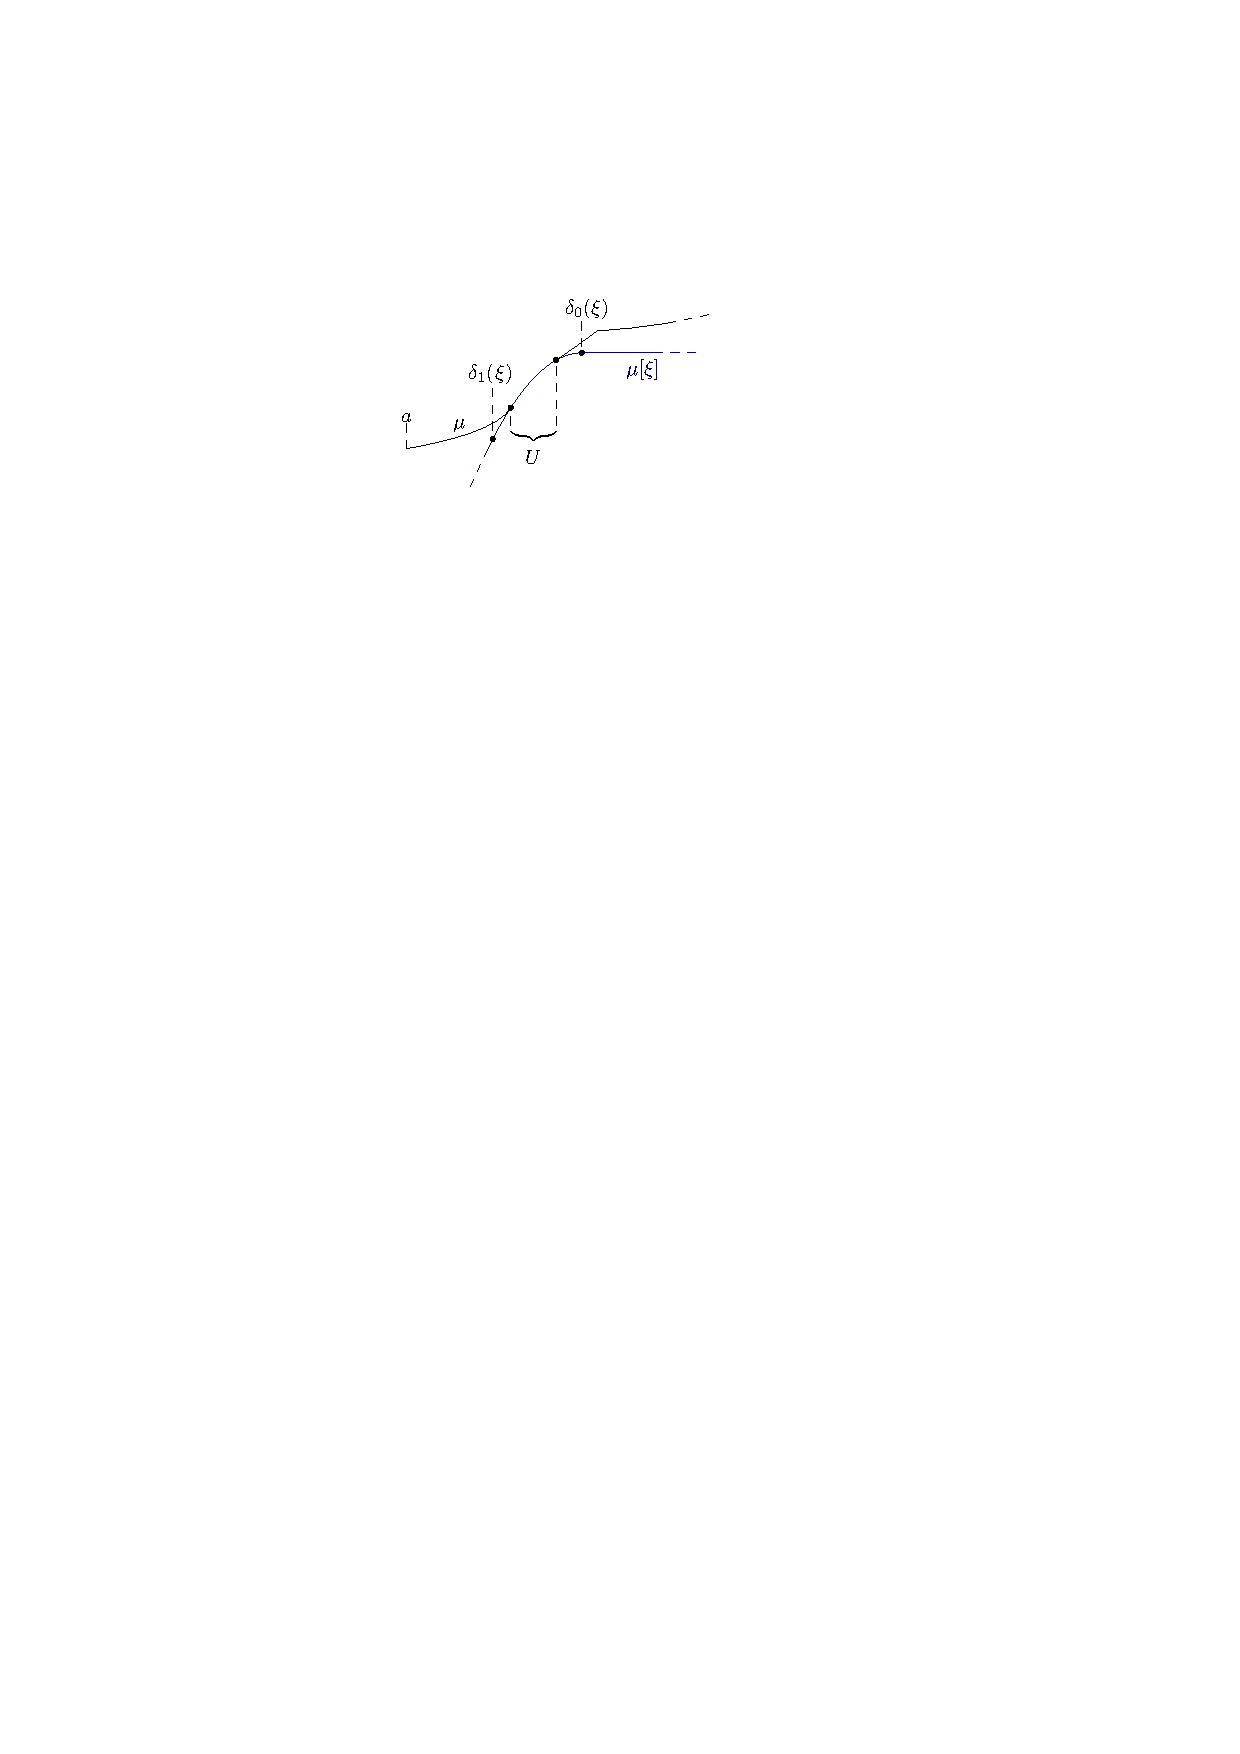
\includegraphics[scale=1.1]{figures/motion/deceleration-boundary-unique}
  \caption{Example of a piecewise trajectory $\mu$ with a part of full
    deceleration over some interval $U$ such that any choice of $\xi \in U$
    produces the same deceleration boundary $\mu[\xi]$, which naturally
    coincides with $\mu$ on $U$.}
  \label{fig:deceleration-boundary-unique}
\end{figure}

Since $X$ is a closed interval, we may define $\xi_{0} = \min X$.
%
Consider any $\xi' \in X$ with $\xi' > \xi_{0}$, then we show $\mu[\xi'](t) = \mu[\xi_{0}](t)$ for all
$t \in [\xi_{0}, b]$. For sake of contradiction, suppose there is some $t' \in [\xi_{0}, b]$ such that
$\mu[\xi'](t') > \mu[\xi_{0}](t')$, then there must be some open interval $U \subset (\xi_{0}, \xi')$ such that
\begin{align}\label{eq:positive-partial-derivative}
  \frac{\partial}{\partial \xi}\mu[\xi](t') > 0 \text{ for all } \xi \in U .
\end{align}
However, we argued in the previous paragraph that this actually holds for any
$t' \geq \delta_{1}(\xi)$.
%
In particular, let $t^{*} \in [t_{1}, b]$ be such that
$\mu(t^{*}) = \mu[\xi_{0}](t^{*})$, then
$t^{*} \geq t_{1} \geq \xi \geq \delta_{1}(\xi)$,
so~\eqref{eq:positive-partial-derivative} yields $\mu[\xi'](t^{*}) > \mu[\xi_{0}](t^{*})$, but then
$d(\xi') > d(\xi_{0}) = 0$, so $\xi' \notin X$, a contradiction.


\paragraph{Touching tangentially.}
%
It remains to show that $\mu$ and $\mu[\xi_{0}]$ touch tangentially somewhere on
$[t_{1}, b]$. Let $\tau_{1} \in [t_{1}, b]$ be the smallest time such that
$\mu(\tau_{1}) - \mu[\xi_{0}](\tau_{1}) = d(\xi_{0}) = 0$ and consider the
following three cases.

First of all, note that $\tau_{1} = t_{1}$ is not possible, because this
would require
\begin{align}
  \dot{\mu}(t_{1}^{+}) > \dot{\mu}[\xi_{0}](t_{1}^{+}) = \dot{\mu}[\xi_{0}](t_{1}) ,
\end{align}
but since $\mu$ is a piecewise trajectory, we must have
$\dot{\mu}(t_{1}^{-}) > \dot{\mu}(t_{1}^{+}) > \dot{\mu}[\xi_{0}](t_{1})$. This
shows that $\mu(t_{1} - \epsilon) < \mu[\xi_{0}](t_{1} - \epsilon)$, for
some small $\epsilon > 0$, which contradicts $\mu[\xi_{0}] \preceq \mu$.

Suppose $\tau_{1} \in (t_{1}, b)$, then recall the definition of $d(\xi_{0})$
and observe that the usual first-order necessary condition (derivative zero) for
local minima requires $\dot{\mu}(\tau_{1}) = \dot{\mu}[\xi_{0}](\tau_{1})$.

Finally, consider $\tau_{1} = b$.
%
Observe that $\dot{\mu}(b) > \dot{\mu}[\xi_{0}](b)$, would contradict
minimality of $\tau_{1} = b$. Therefore, suppose
$\dot{\mu}(b) < \dot{\mu}[\xi_{0}](b)$, then
$\dot{\mu}[b](b) = \dot{\mu}(b) < \dot{\mu}[\xi_{0}](b)$, so
\begin{align}
  \dot{\mu}[b](t) \leq \dot{\mu}[\xi_{0}](t) \text{ for } t \leq b ,
\end{align}
but then $\mu[b](t) > \mu[\xi_{0}](t)$ for $t < b$. In particular, for $t=\xi_{0}$, this shows
$\mu[b](\xi_{0}) > \mu[\xi_{0}](\xi_{0}) = \mu(\xi_{0})$, which contradicts part $\mu[b] \preceq \mu$ of
Assumption~\ref{assump:smoothing}.


\paragraph{Repeat for remaining discontinuities.}
Let us summarize what we have established so far.
%
The times $\xi_{0} \in \halfopen{a}{t_{1}}$ and
$\tau_{1} \in \openhalf{t_{1}}{b}$ have been chosen such that
\begin{subequations}\label{eq:smoothing-requirements}
\begin{gather}
  \mu[\xi_{0}](t) \leq \mu(t) \; \text{ for } \; t \in [\xi_{0}, \tau_{1}] , \\
  \dot{\mu}[\xi_{0}](\xi_{0}) = \dot{\mu}(\xi_{0}) \; \text{ and } \; \dot{\mu}[\xi_{0}](\tau_{1}) = \dot{\mu}(\tau_{1}) .
\end{gather}
\end{subequations}
Instead of $\xi_{0}$, it will be convenient later to choose $\xi_{1} := \max X$
as the representative of the unique connecting deceleration.
%
We can now use $(\mu[\xi_{1}])|_{[\xi_{1},\tau_{1}]}$ to replace $\mu$ at $[\xi_{1}, \tau_{1}]$ to
obtain a trajectory without the discontinuity at $t_{1}$. More precisely, we
define
\begin{align}
  \mu_{1}(t) =
  \begin{cases}
    \mu(t) &\text{ for } t \in [a, \xi_{1}] \cup [\tau_{1}, b] , \\
    \mu[\xi_{1}](t) &\text{ for } t \in [\xi_{1}, \tau_{1}] .
  \end{cases}
\end{align}
From the way we constructed $\mu[\xi_{1}]$, it follows
from~\eqref{eq:smoothing-requirements} that we have
$\mu_{1} \in \mathcal{P}[a,b]$, but without the discontinuity at $t_{1}$.
%
Observe that a single connecting deceleration may cover more than one
discontinuity, as illustrated in Figure~\ref{fig:multiple-discontinuities}.
%
Note that we must have $\dot{\mu}_{1}(a) = \dot{\mu}(a)$ and
$\dot{\mu}_{1}(b) = \dot{\mu}(b)$ by construction.
%
Hence, it is not difficult to see that $\mu_{1}$ must still satisfy
Assumption~\ref{assump:smoothing}, so that we can keep repeating the exact same
process, obtaining connecting decelerations $(\xi_{2}, \tau_2), (\xi_{3}, \tau_{3}), \,\dots$
and the corresponding piecewise trajectories $\mu_{2}, \mu_{3}, \,\dots$ to remove any
remaining discontinuities until we end up with a smooth trajectory
$\mu^{*} \in \mathcal{D}[a,b]$.
%
We emphasize again that $\dot{\mu}^{*}(a) = \dot{\mu}(a)$ and
$\dot{\mu}^{*}(b) = \dot{\mu}(b)$.

\begin{figure}
  \centering
  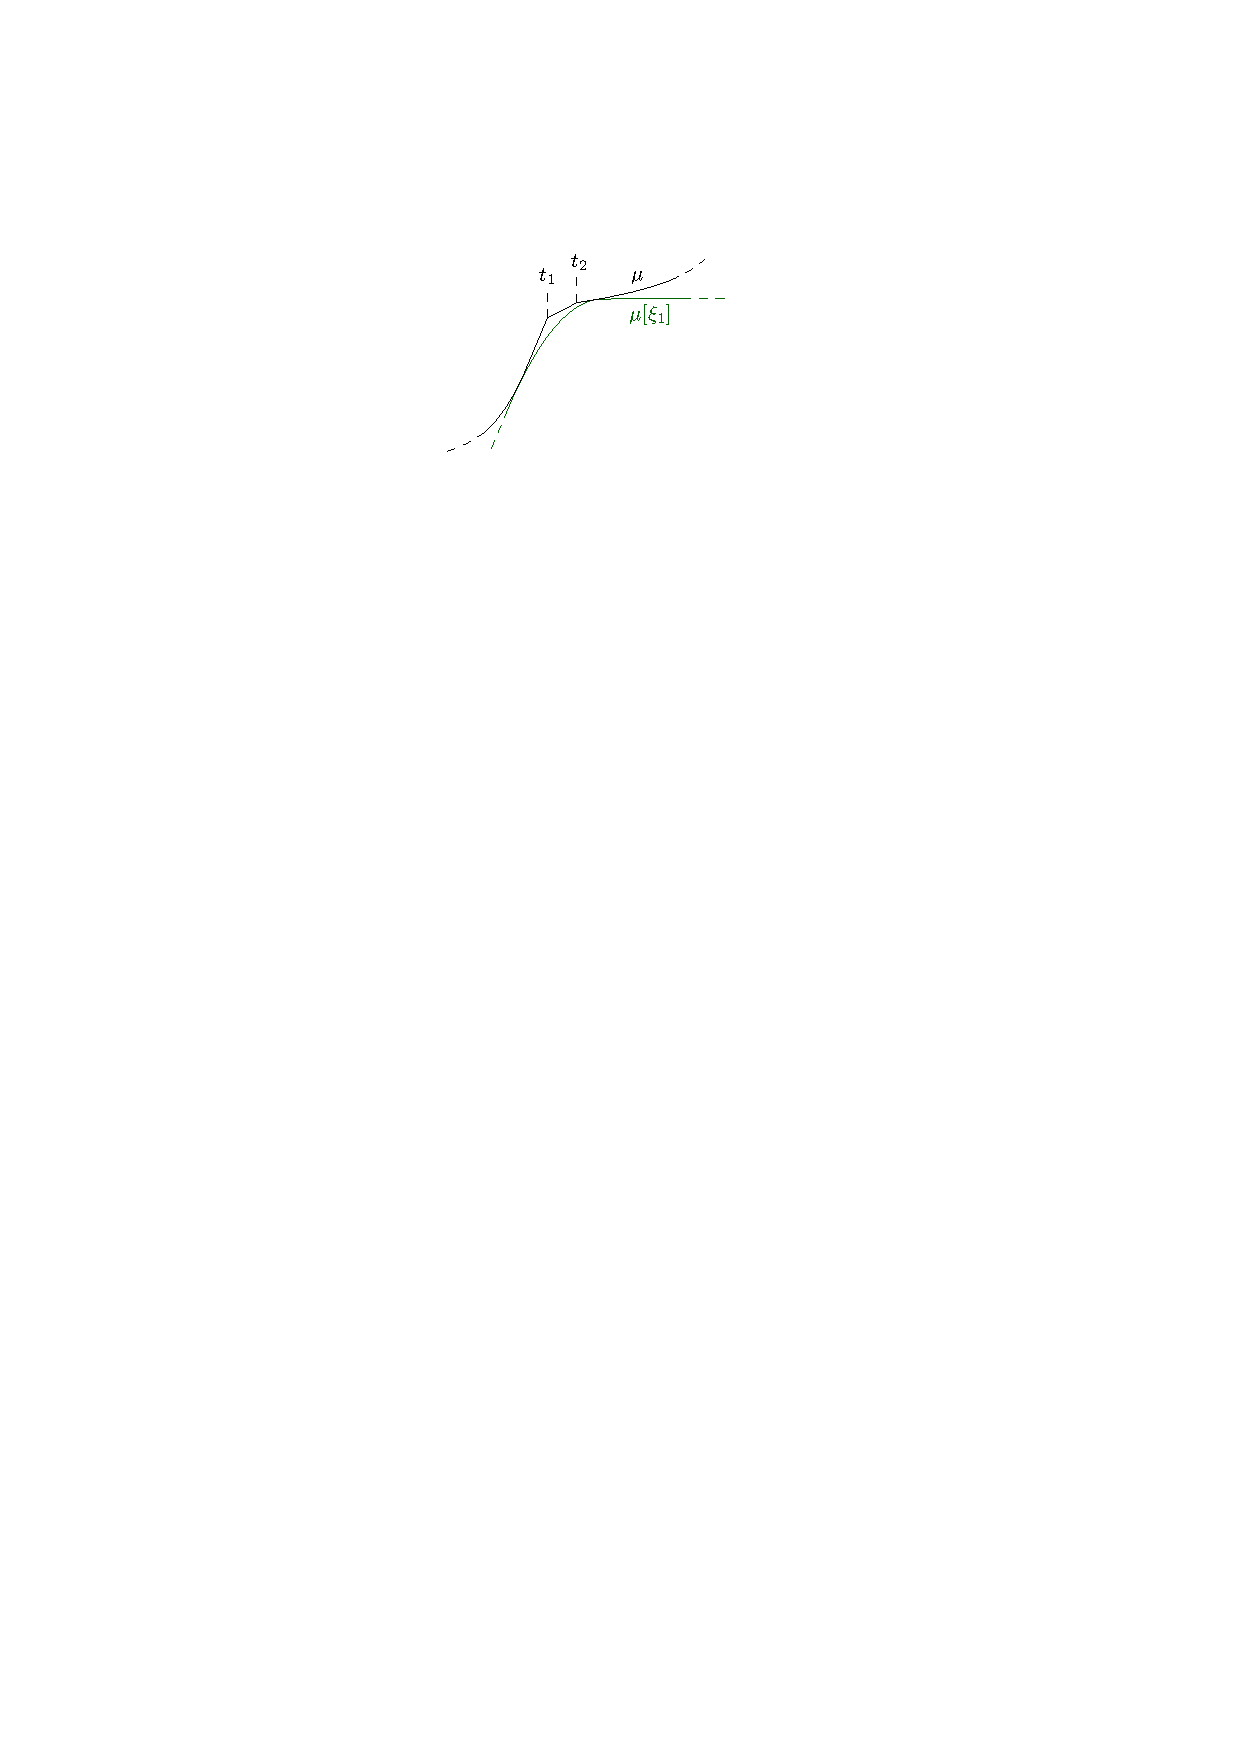
\includegraphics[scale=1.0]{figures/motion/multiple-discontinuities}
  \caption{Part of a piecewise trajectory $\mu$ on which a single connecting
    deceleration covers the two discontinuities at $t_{1}$ and $t_{2}$ at
    once.}%
  \label{fig:multiple-discontinuities}
\end{figure}

\paragraph{Proof of Theorem~\ref{thm:single-vehicle}.}
Let us now return to the minimum boundary $\gamma$ defined
in~\eqref{eq:min-boundary}.
%
From Figure~\ref{fig:necessary-conditions} and the conditions of
Theorem~\ref{thm:single-vehicle}, it is clear that $\gamma$ must satisfy
$\gamma(a) = A$, $\gamma(b) = B$ and 
$\dot{\gamma}(a) = \dot{\gamma}(b) = 1$, so whenever we have
$\gamma \in \mathcal{D}[a, b]$, i.e., $\gamma$ does not contain discontinuities,
we automatically have $\gamma \in D_{2}[a,b]$ so that $\gamma$ itself is already
a feasible solution.
%
%
Otherwise, we perform the smoothing procedure presented above to obtain the
smoothed trajectory $\gamma^{*} \in \mathcal{D}[a,b]$.
%
This completes the proof of Theorem~\ref{thm:single-vehicle}.

\subsection{Upper boundary solution}\label{sec:upper-bound-property}

As a byproduct of the above analysis, the next lemma shows that the solution
$\gamma^{*}$ is also an upper boundary for any other feasible trajectory.

\begin{lemma}\label{lemma:upperbound}
  Let $\mu \in \mathcal{P}[a,b]$ be a piecewise trajectory and let
  $\mu^{*} \in \mathcal{D}[a,b]$ denote the result after smoothing. All
  trajectories $x \in \mathcal{D}[a, b]$ that are such that
  $x \preceq \mu$, must satisfy $x \preceq \mu^{*}$.
\end{lemma}
\begin{proof}
  Consider some interval $(\xi, \tau)$ where we introduced some connecting
  deceleration boundary. Suppose there exists some $t_{d} \in (\xi, \tau)$ such that
  $x(t_{d}) > \mu(t_{d})$. Because $x(\xi) \leq \mu(\xi)$, this means that $x$ must
  intersect $\mu$ at least once in $\halfopen{\xi}{t_{d}}$, so let
  $t_{c} := \sup \, \{ t \in \halfopen{\xi}{t_{d}} : x(t) = \mu(t) \}$ be the latest
  time of intersection such that $x(t) \geq \mu(t)$ for all $t \in [t_{c}, t_{d}]$.
  There must be some $t_{v} \in [t_{c}, t_{d}]$ such that $\dot{x}(t_{v}) > \dot{\mu}(t_{v})$,
  otherwise
  \begin{align*}
    x(t_{d}) = x(t_{c}) + \int_{t_{c}}^{t_{d}} \dot{x}(t) \diff t \leq \mu(t_{c}) + \int_{t_{c}}^{t_{d}} \dot{\mu}(t) \diff t = \mu(d_{t}) ,
  \end{align*}
  which contradicts our choice of $t_{d}$. Hence, for every
  $t \in [t_{v}, \tau]$, we have
  \begin{align*}
    \dot{x}(t) \geq \dot{x}(t_{v}) - \omega (t - t_{v}) > \dot{\mu}(t_{v}) - \omega(t - t_{v}) = \dot{\mu}(t) .
  \end{align*}
  It follows that $x(\tau) > \mu(\tau)$, which contradicts the assumption
  $x \preceq \mu$.
\end{proof}

\begin{remark}
  The above upper boundary property has the following interesting consequence if
  we extend the single vehicle problem to the optimal control of maximizing the
  haste criterion, which was defined as
  \begin{align}\label{eq:haste-objective}
  J(x_{i}) = \int_{a_{i}}^{b_{i}} - x_{i}(t) \diff t .
  \end{align}
  %
  Roughly speaking, this objective seeks to keep all vehicles as close to the end
  of the lane at all times, but it does not capture energy efficiency in any way.
  % 
  In particular, observe that it follows from the above lemma that any other
  $x \in D_{2}[a,b]$ satisfying $x \preceq u$ must also satisfy
  \begin{align}
    \int_{a}^{b} x(t) \diff t \leq \int_{a}^{b} \gamma^{*}(t) \diff t
  \end{align}
  Consequently, $x = \gamma^{*}$ is an optimal solution to the single vehicle
  optimal control problem
  \begin{align}
    \max_{x \in D_{2}[a,b]} J(x) \; \text{ such that } \; x \preceq u .
  \end{align}

\end{remark}


\section{Lane planning feasibility}\label{sec:lane-problem-feasibility}

We will now return to the feasibility of the lane planning problem and show how
it decomposes in terms of a sequence of single vehicle feasibility problems.
%
Let us first restate the conditions for feasible solutions of the lane planning
problem.
%
Recall that we are given schedule times $a = (a_{1}, a_{2}, \dots, a_{N})$ and
$b = (b_{1}, b_{2}, \dots, b_{N})$, which are assumed to be ordered as
$a_{1} \leq \dots \leq a_{N}$ and
$b_{1} \leq \dots \leq b_{N}$.
%
For brevity, we will write $x \in D_{2}^{N}[a, b]$ to denote the vector
$x = (x_{1}, \dots, x_{N})$ of $N$ trajectories $x_{i} \in D_{2}[a_{i},b_{i}]$.
%
Assume the system parameters $(\omega, \bar{\omega},A,B,L)$ to be fixed, then
the goal is to find a sequence of trajectories $x \in D_{2}^{N}[a,b]$ such that
\begin{subequations}
\begin{alignat}{2}
  &x_{i} \in D_2[a_{i},b_{i}] && \quad \text{ for each } i \in \{1, \dots, N\} , \\
  &x_{i} \preceq x_{i-1} - L && \quad \text{ for each } i \in \{2, \dots, N\} . \label{eq:follow-constraint}
\end{alignat}
\end{subequations}

%
The general idea is to repeat the construction of the previous section for each
vehicle to obtain a solution $x_{i}$, while using each constructed trajectory as
the boudary $u = x_{i}$ for the next problem of finding $x_{i+1} \preceq u$.
%
We will show that feasibility is equivalent to having the schedule times $a_{i}$
and $b_{i}$ satisfy a certain system of inequalities.
%
We will need the following technical assumption regarding the minimum length of
the lane, which is very reasonable to assume in practice.

\begin{assump}\label{assump:L-bound}
  Assume that vehicle lengths are limited by $L < B - A$.
\end{assump}

\begin{figure}
  \centering
  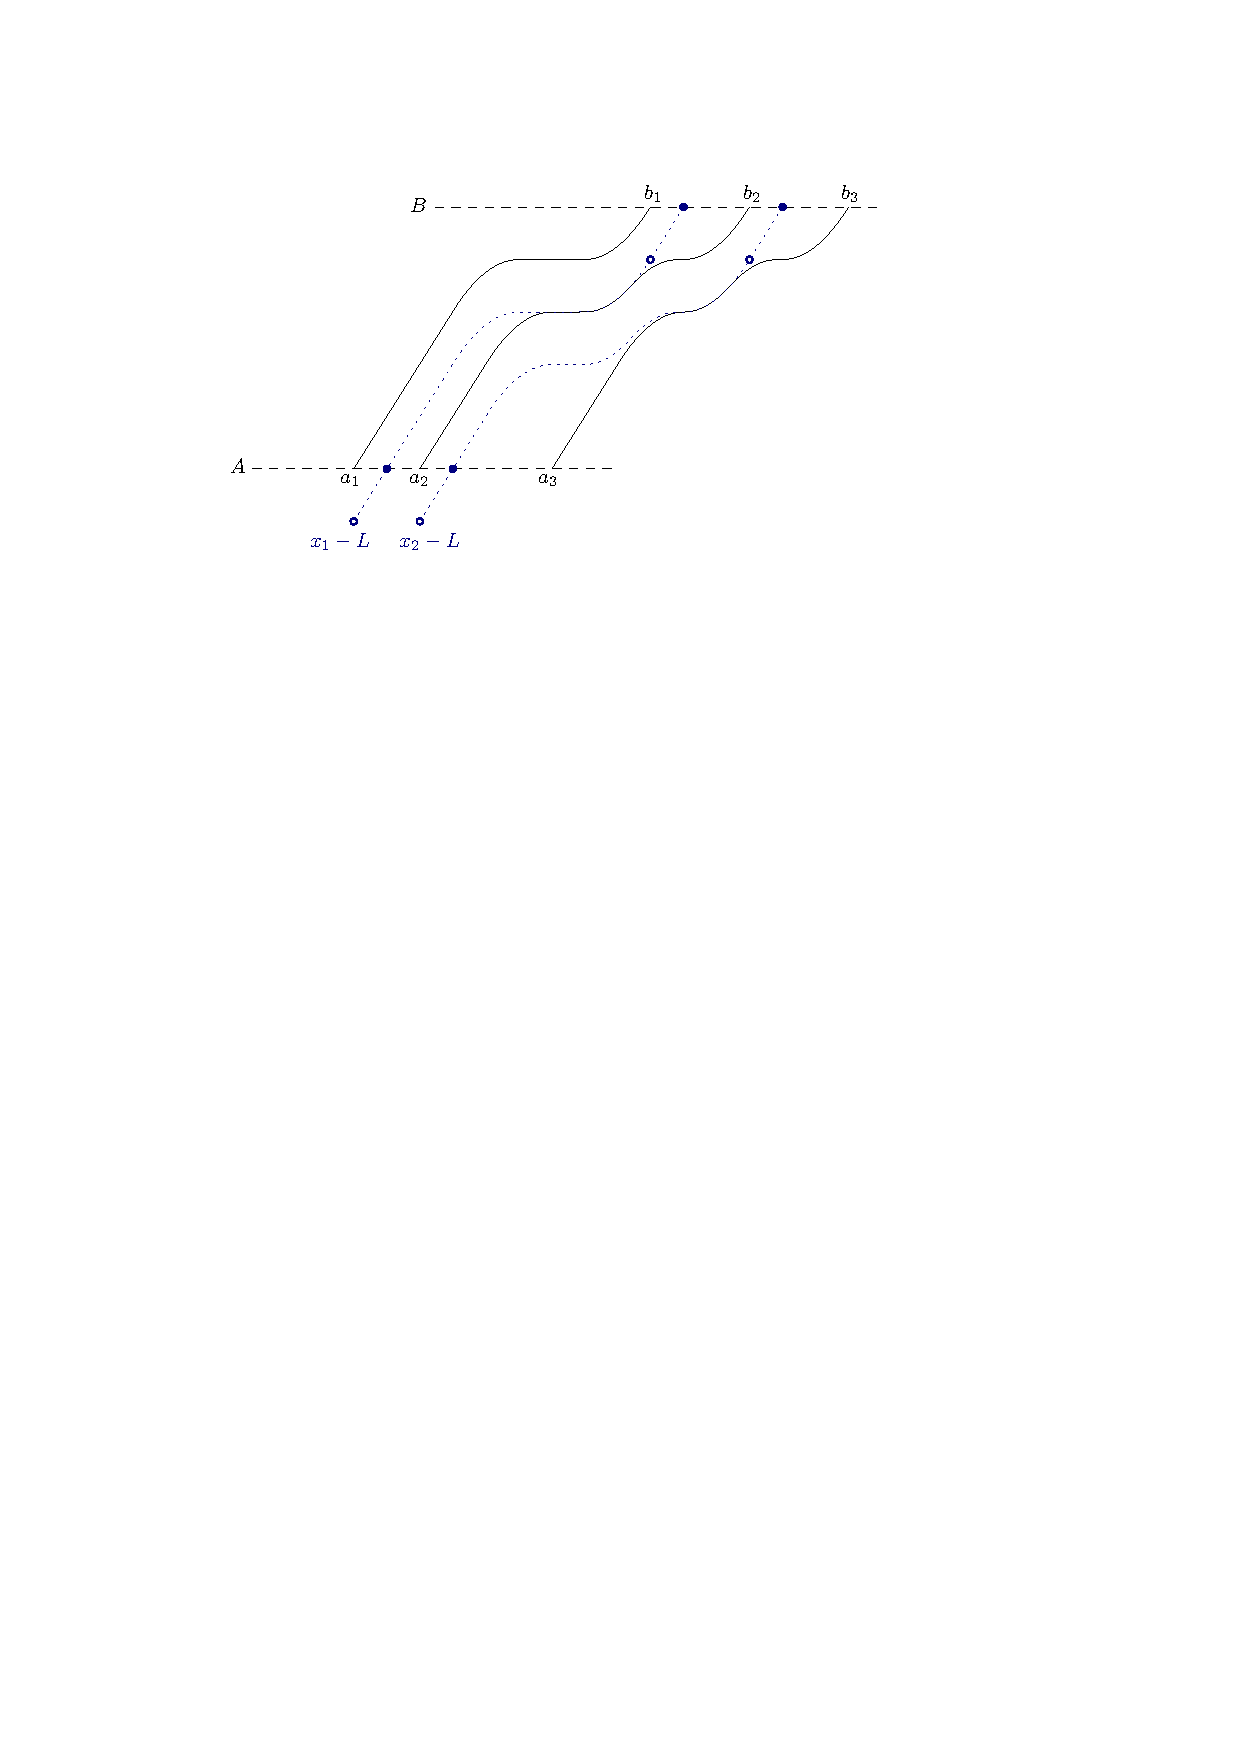
\includegraphics[scale=1.0]{figures/motion/solution}
  \caption{Optimal trajectories $x_{i}$ for three vehicles. The dotted blue
    trajectories between the little open circles illustrates the safe following
    constraints~\eqref{eq:follow-constraint}. The dotted blue trajectories between
    the solid dots are the following boundaries
    $\bar{x}_{2} \in \bar{D}[\bar{a}_{2}, \bar{b}_{2}]$ and
    $\bar{x}_{3} \in \bar{D}[\bar{a}_{3}, \bar{b}_{3}]$.}%
  \label{fig:solution}
\end{figure}

Now consider the safe following constraints~\eqref{eq:follow-constraint}.
%
We show how transform these into equivalent upper boundaries
$\bar{x}_{i} \in \bar{D}_{1}[\bar{a}_{i}, \bar{b}_{i}]$ for each
$i \in \{2, \dots, N\}$, such we can apply Theorem~\ref{thm:single-vehicle}.
%
It becomes clear from Figure~\ref{fig:solution} that
inequality~\eqref{eq:follow-constraint} only applies on some subinterval
$I_{i} \subset [a_{i-1}, b_{i-1}]$.
%
However, as the figure suggests, we can easily truncate and extend these
boundaries as necessary.
%
For some $y \in \mathcal{D}[\alpha, \beta]$, we define the inverse at some
position $p$ in its range to be
\begin{align}
  y^{-1}(p) = \inf \{ t \in [\alpha, \beta] : y(t) = p\} .
\end{align}
%
Given some trajectory $u \in D_{1}[c,d]$, we define its \emph{downshift}
%
\begin{align}
  \bar{u}(t) =
  \begin{cases}
    u(t) - L &\text{ for } t \in [u^{-1}(A + L), d] , \\
    B - L + t - d &\text{ for } t \in [d, d + L] .
  \end{cases}
\end{align}
For ease of reference, we denote the endpoints of its domain as
$\bar{a} := u^{-1}(A+L)$ and $\bar{b} := d + L$.

\begin{lemma}[Boundary extension]\label{lemma:boundary-extension}
  Consider some trajectory $u \in \mathcal{D}[c,d]$ such that $u(d) \geq A$. If
  $x \in \mathcal{D}[a,b]$ is such that $x(a) = A$ and $x \preceq u$, then it
  satisfies $x \preceq (u(d) + t - d)|_{\halfopen{d}{\infty}}$, which may be
  interpreted as extending the upper boundary $u$ to the right at full speed.
\end{lemma}
\begin{proof}
  If $b < d$, then $x \preceq (\cdot)|_{\halfopen{d}{\infty}}$ is always void and
  the statement is trivially true. Assume $b \geq d$ and consider an arbitrary
  $t \geq d$.
  %
  Suppose $a \leq d$, then we have $x(t) \leq x(d) + t - d \leq u(d) + t - d$.
  Suppose $a > d$, then we have $x(t) \leq x(a) + t - a = A + t - a \leq u(d) + t - d$.
\end{proof}
\begin{lemma}[Downshift boundary equivalence]\label{lemma:downshift}
  For each $u \in D_{2}[c,d]$, the downshift trajectory satisfies
  $\bar{u} \in D_{1}[\bar{a},\bar{b}]$.
  %
  For each $x \in D[a, b]$ such that $a \geq c$ and $b \geq d$, we have
  $x \preceq u - L$ if and only if $x \preceq \bar{u}$.
\end{lemma}
\begin{proof}
  The two cases in the definition of $\bar{u}$ coincide, so that
  $\bar{u} \in \mathcal{D}$. Furthermore, it is easily verified that
  $\bar{u}(\bar{a}) = A$ and $\bar{u}(\bar{b}) = B$, so the first claim
  follows.

  Suppose $x \preceq u - L$, and suppose there exists some
  $t \in [a,b] \cap [c,d]$. If $t \in [\bar{a}, d]$, then
  $x(t) \leq u(t) - L = \bar{u}(t)$ by definition. If $t \in [d, \bar{b}]$, then
  apply Lemma~\ref{lemma:boundary-extension} to $u - L$ (using
  Assumption~\ref{assump:L-bound} for $u(d) - L \geq A$) to obtain
  $x \leq (\tau \mapsto u(d) - L + \tau - d)|_{\halfopen{d}{\infty}} = (\tau \mapsto B - L + \tau - d)|_{\halfopen{d}{\infty}}$,
  so that $x(t) \leq B - L + t - d = \bar{u}(t)$.

  For the other direction, suppose $x \preceq \bar{u}$. First of all, since
  $u(c) = A$ and $u(\bar{a}) = A+L > A$ and $u$ is non-decreasing, we have
  $c < \bar{a}$.
  %
  Suppose $c \leq a < \bar{a}$, then since $b \geq d \geq \bar{a}$ and
  $\dot{x}(a) = 1$, we must have
  $x(\bar{a}) > x(a) = A = \bar{u}(\bar{a})$, contradicting the initial
  assumption.
  %
  Hence, $a \geq \bar{a}$, so any $t \in [a,b] \cap [c,d]$ satisfies
  $t \in [\bar{a}, d]$, but then $x(t) \leq \bar{u}(t) = u(t) - L$ by
  definition.
\end{proof}

%
The following lemma summarizes what we have established so far.

\begin{lemma}\label{lemma:summary}
  The following four statements are equivalent:

  \begin{enumerate}[leftmargin=3em]
    \item[(C0)] The lane planning problem is feasible.
    \item[(C1)] There exists $x \in D_{2}^{N}[a, b]$ such that $x_{i} \preceq x_{i-1} - L$ for all $i \in \{2, \dots, N\}$.
    \item[(C2)] There exists $x \in D_{2}^{N}[a, b]$ such that $x_{i} \preceq \bar{x}_{i-1}$ for all $i \in \{2, \dots, N\}$.

    \item[(C3)] There exists $x \in D_{2}^{N}[a, b]$ such that
          $b_{i} - a_{i} \geq B - A$ for all $i \in \{1, \dots, N\}$; and
    \TabPositions{2cm}
    \begin{enumerate}[label=(\roman*)\quad,leftmargin=3em,midpenalty=10]
      \item $b_{i} \geq \bar{b}_{i-1}$, \tab (exit order constraint)
      \item $a_{i} \geq \bar{a}_{i-1}$, \tab (entry order constraint)
      \item $\bar{x}_{i-1} \succeq \check{x}_{i}$, \tab (entry space constraint)
    \end{enumerate}
    for all $i \in \{2, \dots, N\}$.

  \end{enumerate}
\end{lemma}
\begin{proof}
  Of course, (C0) and (C1) are equivalent by definition of the lane planning
  problem. Note that equivalence of (C1) and (C2) is handled by Lemma~\ref{lemma:downshift}.
  %
  Equivalence of (C2) and (C3) follows from a straightforward application of
  Theorem~\ref{thm:single-vehicle} by setting $x=x_i$ and $u=\bar{x}_{i-1}$ for
  each $i \in \{2, \dots, N\}$.
\end{proof}

\paragraph{Conjecture: simpler conditions.}
Our next goal is to get rid of the entry space constraints and replace them
with an inequality constraints in terms of schedule times.
%
Moreover, we want to get rid of the dependence of $\bar{a}_{i-1}$ on
$\bar{x}_{i-1}$, such that we obtain equivalent statements in $a_{i-1}$. Note
that the exit order constraint is already in the desired form, because we have
$\bar{b}_{i-1} = b_{i-1} + L$.
%
More specifically, we want to show that the statements of
Lemma~\ref{lemma:summary} above are further equivalent to:

\begin{enumerate}[leftmargin=3em]
  \item[(C4)] $b_{i} - a_{i} \geq B-A$ for all $i \in \{1, \dots, N\}$; and
  \begin{enumerate}[leftmargin=4em,midpenalty=10]
    \item[(i*)\quad] $b_{i} \geq b_{i-1} + L$,
    \item[(ii*)\quad] $a_{i} \geq a_{i-1} + L$,
  \end{enumerate}
  \TabPositions{3cm}
  for all $i \in \{2, \dots, N\}$; and
  \begin{enumerate}[leftmargin=4em,midpenalty=10]
    \item[(c*)\quad] $a_{i} \geq \check{a}_i(a,b)$, \tab (entry time constraint)
  \end{enumerate}
  for all $i \in \{n, \dots, N \}$,
\end{enumerate}
for some $n \geq 2$ and where $\check{a}_{i}(a,b)$ denotes some expression in terms of
schedule times. Consequently, $\max\{a_{i-1} + L, \check{a}_{i}(a,b)\}$ can be
interpreted as the earliest possible time of arrival to the lane for vehicle
$i$.

Before we are able to prove this equivalence, we need some better understanding
of the smoothing procedure, which means that try to derive explicit formulas for
finding the touching times $\xi$ and $\tau$ to obtain optimal trajectories under
the haste objective.
%
This will be the subject of further research.


\section{Notes and references}

The analysis of feasibility conditions in this chapter is very much related to
the proof of the safety guarantee in~\cite{miculescuPollingsystemsbasedAutonomousVehicle2016}, see their Lemma IV.4 with
relatively long proof in appendix.
%
They study the online situation, in which new vehicles arrive to the system at
later times, for which they show that the rescheduling policy is safe, in the
sense that there are still feasible and collision-free trajectories for the
vehicles whose crossing times got updated.
%
We do not study such an online setting, but we take into account the fact that
lanes are of finite length.

We emphasize that the assumption $\dot{x}(a) = \dot{x}(b) = 1$ was mainly made
for convenience.
%
There are different ways of relaxing the state constraints on the speed that
could be studied.
%
The interesting question is whether feasibility can still be easily characterized.
%
Instead of fixing the speed to be maximal at entry and exit, we could require,
for example, that the speed is bounded from below, i.e., $\eta \leq \dot{x}(a) \leq 1$
and $\eta \leq \dot{x}(b) \leq 1$, for some $\eta > 0$.
%
The motivation for studying this relaxation is that this might lead to more
energy efficient trajectories, whenever full speed crossing is not strictly
necessary.


% \addtocontents{toc}{\protect\renewcommand\cftbeforechapskip{2.5em}}
\chapter{Conclusion and discussion}\label{chap:conclusion}
\addtocontents{toc}{\protect\renewcommand\cftbeforechapskip{1em}}

The coordination of autonomous vehicles at intersections is a challenging
optimization problem that has been approached from many perspectives across
different research communities---each bringing their own modeling paradigms and
solution methodologies.
%
In this thesis, we have taken a deliberately simplified yet rigorous
mathematical optimization perspective, focusing on understanding the fundamental
computational challenges that arise even in idealized settings.
%
By abstracting away from many practical complexities---such as unobservability,
decentralized control, and mixed traffic---we have been able to isolate and
analyze a core computational difficulty: \emph{the joint optimization of discrete
crossing order decisions and continuous-time vehicle trajectories}.

Starting with a single intersection model, we identified a key structural
property of this problem.
%
A central theme has been the decomposition of the joint optimization into more
manageable components: an upper-level scheduling problem that determines when
vehicles cross intersections, and lower-level trajectory generation problems
that compute the actual vehicle paths.
%
Under specific assumptions---particularly that vehicles cross intersections at
full speed and that delay minimization is the primary objective---we showed that
this decomposition becomes proper, reducing an infinite-dimensional trajectory
optimization problem to a \emph{combinatorial scheduling problem}.

This reduction opened the door to applying both classical optimization
techniques and modern machine learning approaches.
%
We demonstrated how mixed-integer linear programming can solve small to
medium-sized instances optimally, while learning-based constructive heuristics
offer a promising path forward.
%
The conceptual framework developed for the single intersection
case---particularly the formulation as a MDP for learning-based
scheduling---provides a foundation that could scale to networks of
intersections, though this extension introduces additional challenges that merit
further investigation.
%
Below, we reflect on the contributions of this work, discuss its limitations,
and outline directions for future research that could help bridge the gap
between our idealized models and real-world autonomous traffic management
systems.

\section{Contributions}

\paragraph{Motion planning model with direct transcription baseline.}
We formulated a simple model of a single intersection and provided a simple
extension to networks of intersections.
%
We formulated safe motion planning as a problem of trajectory optimization with
collision-avoidance constraints.
% direct transcription does not scale
Within this framework, we studied two approaches to safe motion planning.
%
First of all, we showed that the collision-avoidance constraints can be directly
encoded within the context of direct transcription to an integer program,
yielding an immediate solution for safe motion planning in the single
intersection, as well as networks of intersections.

Although this method is easy to implement and it guarantees to find optimal
solutions (up to time discretization) that are provably safe, it scales very
poorly to larger instances.
%
Hence, without further changes, it is not a good candidate for enabling
large-scale coordination in networks.
%
This issue is the main motivation for our concrete proposals.

\paragraph{Decomposition and improved integer programming.}
As an alternative to direct transcription, we discussed the technique of
separating the decisions regarding occupancy time slot reservations.
%
Although the decomposition itself does not immediately provide better
algorithms, we stress that it is a useful conceptual tool, as previously
demonstrated by data-driven approximation
methods~\cite{hultApproximateSolutionOptimal2015,hultTechnicalReportApproximate}.
% mild assumptions -> provably safe + potential to scale
Instead of keeping the optimality guarantees, we choose to make some simplifying
assumptions in favor of a proper decomposition, which then leads to a provably
safe coordination scheme that has far better potential for scaling up.

% exploiting optimal structure
Based on the proper decomposition, we can focus on solving the resulting
crossing time scheduling problem. Integer programming provides a readily
available and mature solution.
%
It can handle single intersection problems fairly well, but computing optimal
solutions becomes expensive ($>$1 minute of computation time) for more than 20
vehicles.
%
Nevertheless, modern solvers provide a pretty good heuristic when computation
time is limited.
% cutting planes
To further improve the applicability of integer programming, we show how a
particular structure in optimal schedules leads to the natural formulation of
three types of cutting planes.
%
We show that one type of cuts clearly improves the running time and increases
the size of instances that we can solve roughly by a factor 4.


\paragraph{Hand-crafted and machine-learned constructive heuristics.}

As an alternative to integer programming, we explored the feasibility of using a
constructive scheduling approach for solving the crossing time problem.
%
We defined a Markov decision process that simulates a constructive step-by-step
schedule building process for the single intersection problem.
%
There exists a redundancy in this natural formulation, which led us to propose a
state abstraction function, resulting in a significant reduction of the state
space.

Policies based on a very elementary rule already provide a very good heuristics
that is computationally very cheap, demonstrating the effectiveness of the state
reduction.
%
Furthermore, we illustrate the potential for machine-learned heuristics by
proposing a simple neural policy architecture, where the sequence of upcoming
arrivals of each lane is embedded by a recurrent neural network.
%
We demonstrated two ways of fitting the parameters of this class of policies.
%
When instance sizes still allow us to compute optimal schedules, it seems a good
idea to use the imitation learning setting.
%
For tackling larger instance sizes, the case for reinforcement learning becomes
very strong.

To extend the constructive scheduling method to the network problem, we extended
the action space to also include the decision at which intersection to take the
next step.
%
This introduces additional redundancy. In the imitation learning regime, we
observed that ``order matters'' and confirm our hypothesis that keeping the
amount of progress---in terms of scheduling steps taken---balanced across
intersection, leads to better convergence and final model performance.


\section{Limitations and further work}

\paragraph{Beyond proper decomposition: true joint optimization.}

We believe that full speed crossing and the delay objective are sensible
assumptions from a practitioner's point of view.
%
However, from a methodological standpoint, our setting is not very satisfying.
%
In the general setting, the trajectory optimization problem does not decompose:
the upper- and lower-level problems must be considered simultaneously.
%
We identify the following two issues:

\begin{enumerate}
  \item Feasibility of the lower-level problem is a complicating factor, because
        it puts difficult-to-formalize constraints on the upper-level
        combinatorial problem.
        %
        We wonder how to leverage sampling-based methods to approximate these
        constraints on the time schedule.
        %
        In other words, can we approximate the space of feasible time schedules,
        with guarantees?

  \item In general, the optimization objective is not just a linear function of
        the upper-level decisions variables.
        %
        We would like to see how an data-driven approximation of the objective,
        similar to the proposal
        in~\cite{hultApproximateSolutionOptimal2015,hultTechnicalReportApproximate},
        could be extended to network scheduling.
\end{enumerate}


\paragraph{Discovering structure in optimal network schedules.}

The major limitation of our current network model is the fact that vehicle
routes are fully independent, meaning that traffic can only follow predefined
straight paths.
%
We made this assumption mainly out of computational convenience and for the sake
of a relatively simpler implementation and presentation.
%
Our intuition is that optimal network schedules behave \emph{somewhat like the
  platoon preservation theorem} for single intersections.
%
We say ``somewhat'', because it is quite straightforward to find counterexamples
to the platoon perservation theorem in small networks with only a couple of
intersections.

When the independent route assumption is relaxed, the combinatorial space of
crossing order grows significantly, so following the above intuitive argument,
this means that a lot of feasible solutions are introduced that are clearly
suboptimal.
%
It would be great if this intuitive statement could be captured by a formal
statement, but it is probably too fuzzy.
%
Rather, we would like to push the machine learning perspective, because we
believe this example is an excellent candidate for this paradigm.


\paragraph{Connection with RL for job shop scheduling.}

Very related to our investigation is the huge amount of work that has been done
on neural reinforcement learning methods for job shop scheduling, which is very
related to our network scheduling problem. Hence, this is a highly suggested
direction of further research and collaboration.


% the code around the bibliographp itself serves as
% a sort of anchor for adding a bookmark entry
\phantomsection
\begin{singlespacing}\raggedright
% \bibliographystyle{unsrt}
% \bibliography{references}\label{sec:references}
\printbibliography
\end{singlespacing}
% add entry to documents table of contents
\addcontentsline{toc}{chapter}{Bibliography}

\cleardoublepage\makeatletter\@openrightfalse\makeatother

\appendix


% add '.' after appendices in pdf bookmark, to avoid misreading 'A' as the first
% word of a sentence
% TODO: only do this at the top level
\let\origthechapter\thechapter
\makeatletter
\xpatchcmd{\addcontentsline}{%
\Hy@writebookmark{\csname the#2\endcsname}%
      {#3}%
      {\@currentHref}%
      {\Hy@toclevel}%
      {#1}%
}{%
\begingroup
\renewcommand{\thechapter}{\origthechapter.}
\Hy@writebookmark{\csname the#2\endcsname}%
{#3}%
{\@currentHref}%
{\Hy@toclevel}%
{#1}%
\endgroup
}{\typeout{Success}}{}
\makeatother

% % non-bold appendix entries
% \addtocontents{toc}{\protect
% \renewcommand{\protect\cftchapaftersnumb}{\normalfont}
% }
% % ...also non-bold page numbers
% \addtocontents{toc}{\protect
% \renewcommand{\protect\cftchappagefont}{\normalfont}
% }
% % decrease space between appendix entries
% \addtocontents{toc}{\protect
% \renewcommand{\protect\cftbeforechapskip}{\vskip0pt}
% }


\addtocontents{toc}{\vspace{0.5cm}} % add 0.5 cm space
\part*{Appendix}
% \addcontentsline{toc}{part}{Appendix}

\chapter{Feasible configurations for single intersection model}\label{app:configuration-space}

\begin{figure}
  \centering
  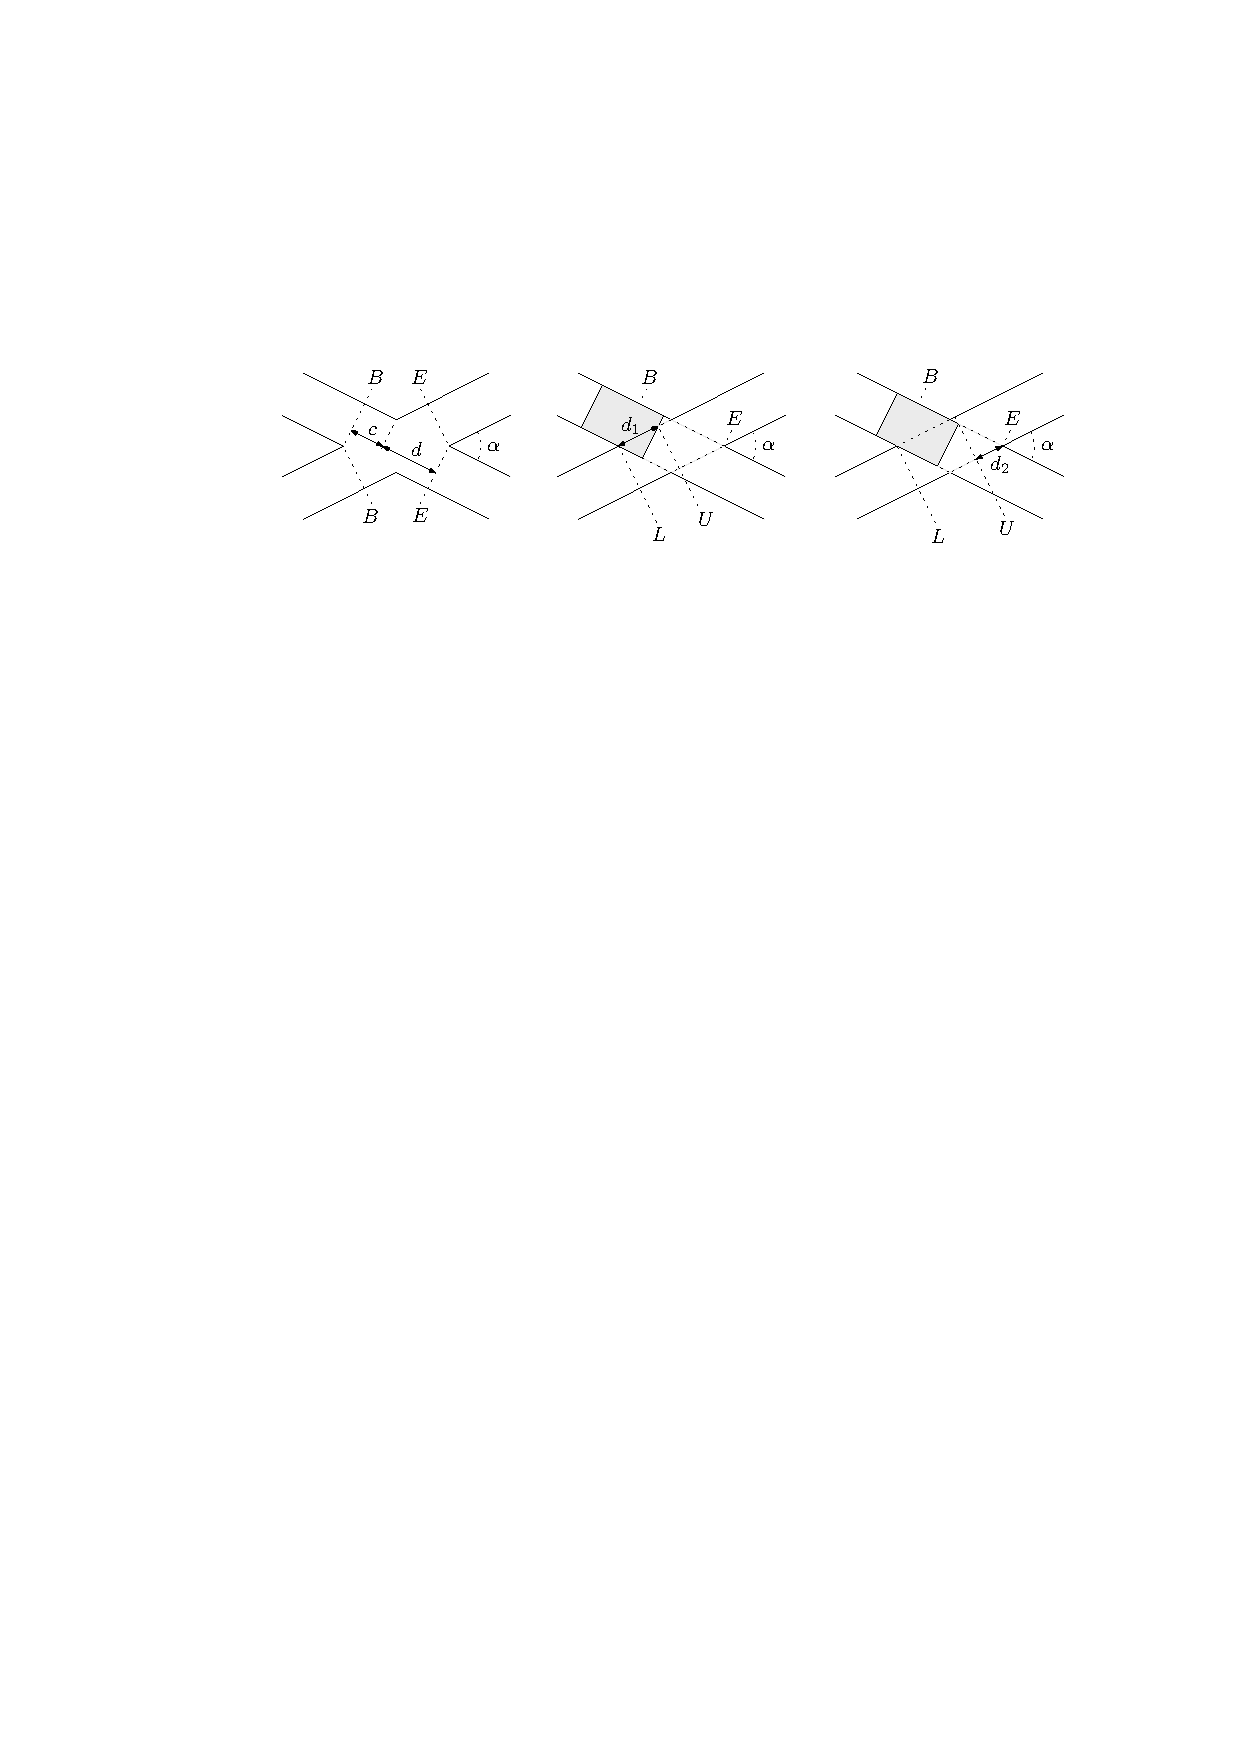
\includegraphics[scale=1]{figures/configuration-space}
  \caption{Sketches to derive the feasible configurations of two vehicles in the
    intersecting routes model. Using some elementary trigonometry, the distances
    in the first figure can be shown to be $c = W / \tan(\alpha)$ and
    $d = W / \sin(\alpha)$. Furthermore, observe that we have
    $(x_{i} - B) / d_{1} = \cos(\alpha)$ for
    $x_{i} \in \openhalf{B}{B + c}$, as shown in the middle figures and
    $d_{2}/(E - x_{i}) = \cos(\alpha)$ for $x_{i} \in \halfopen{B + c}{E}$,
    as shown in the right figure. These two types of distances can be used to
    derive the full characterization.}
  \label{fig:configuration-space}
\end{figure}

We present a way to derive the feasible configurations of the two routes that
intersect at some arbitrary angle, as shown in Figure~\ref{fig:intersection-non-axis-aligned}.
% general case
Assume that $\alpha < \pi / 2$ is the acute angle between the two intersections.
%
Furthermore, we consider uniform rectangular vehicle geometries with
$L_{i} \equiv L$ and $W_{i} \equiv W$, but the analysis is easily extended to
arbitrary dimensions.
%
We skip a thorough derivation of the following expressions, but we note that it
is based on the type of the distances illustrated in
Figure~\ref{fig:configuration-space}.
%
Roughly speaking, we encode the part of the intersection that vehicle $i$
occupies in terms of the other vehicle's $x_{j}$ coordinates, by defining the
following upper and lower limit positions
\begin{align}
  u(x_{i}) &:=
  \begin{cases}
    -\infty & \hspace{1.9em} \text{ if } x_{i} \leq B \text{ or } x_{i} - L \geq E , \\
    B + (x_{i} - E) / \cos(\alpha) & \hspace{1.9em} \text{ if } x_{i} \in \openhalf{E}{E + c\,} , \\
    E + (x_{i} - E) \cdot \cos(\alpha) & \hspace{1.9em} \text{ if } x_{i} \in \halfopen{E + c}{E} , \\
    E & \hspace{1.9em} \text{ if } x_{i} \geq E \text{ and } x_{i} - L < E ,
  \end{cases} \\
  l(x_{i}) &:=
  \begin{cases}
    B & \text{ if } x_{i} - L \leq E \text{ and } x_{i} > E , \\
    B + (x_{i} - L - E) / \cos(\alpha)     & \text{ if } x_{i} - L \in \openhalf{E}{E - c\,} , \\
    E + (x_{i} - L - E) \cdot \cos(\alpha) & \text{ if } x_{i} - L \in \halfopen{E - c}{E} , \\
    \infty & \text{ if } x_{i} - L \geq E \text{ or } x_{i} \leq E .
  \end{cases}
\end{align}
With these definitions, in order for the intersection to be free for vehicle
$j$, position $x_{i}$ must satisfy either $x_{i} < l(x_{j})$ or
$x_{i} - L > u(x_{j})$ and $x_{j}$ must satisfy either $x_{j} < l(x_{i})$ or
$x_{j} - L > u(x_{i})$.
%
Hence, these two pairs of equations completely determine the set of feasible
configurations, which can now be written as
\begin{alignat}{4}
  \mathcal{X}_{ij} = \{ (x_{i}, x_{j}) \in \mathbb{R}^{j} :& \; &&[\,x_{i} - L,x_{i} &]& \cap [\,l(x_{j}), u(x_{j}) &&] = \varnothing \\
  \text{ and } & \, &&[\,x_{j} - L, x_{j} &]& \cap [\,l(x_{i}), u(x_{i}) &&] = \varnothing \} .
\end{alignat}
%
In case the routes intersect at a right angle $\alpha = \pi / 2$, the situation
is much simpler and the two limiting positions are simply given by
\begin{align}
  (l(x_{i}), u(x_{i})) =
  \begin{cases}
    (B,  E)    &\text{ if } (x_{i} - L, x_{i}) \cap (B, E) \neq \varnothing , \\
    (\infty, -\infty) &\text{ otherwise, }
  \end{cases}
\end{align}
such that the set of feasible configurations is simply given by
\begin{align}
  \mathcal{X}_{ij} = \mathbb{R}^{2} \setminus [B,E + L]^{2} .
\end{align}

\chapter{Job shop scheduling}\label{app:job-shop}

The job shop model provides a mathematical framework to study systems where a
given set of---possibly distinct---facilities must be shared among a number of
heterogeneous tasks over time.
%
We begin by providing a fairly general definition of this model and then present a
small example for a specific problem.
%
Next, we introduce the disjunctive graph, which is a standard auxiliary
representation of both problem instances and solutions.
%
Finally, we briefly discuss simple heuristics and illustrate how job shop
problems can be approached within the mixed-integer programming framework.
%
For a comprehensive textbook treatment of job shop scheduling, we refer the
reader to~\cite[Chapter 7]{pinedoSchedulingTheoryAlgorithms2016}.

\paragraph{General definition.}
Originally motivated by production planning problems, the job shop model is
phrased in terms of a set of $n$ jobs that require to be processed on a set of
$m$ machines. Each machine can process at most one job at the same time.
%
We use the pair of indices $(i,j)$ to identify the operation that machine $i$
performs on job $j$, which takes a fixed amount of time $p(i,j)$.
%
Each job $j$ visits all machines\footnote{When some job $j$ requires only
  processing on a proper subset of the machines, observe that we can simply
  assume that $p(i,j) = 0$ for each machine $i$ that is not involved.} following
a predetermined machine sequence, which may be different among jobs.
%
Let $\mathcal{N}$ denote the set of all operations, then the general Job Shop Scheduling
Problem (JSSP) is to determine a schedule $y = \{ y(i,j) : (i,j) \in \mathcal{N} \}$ of
starting times such that some objective function $J(y)$ is minimized.
%
Variants of this basic problem can be obtained by specifying a concrete
objective function and by introducing additional constraints, which we will both
illustrate in the following example.

\begin{eg}\label{eg:job-shop}
  Let $s_{j}$ and $e_{j}$ denote the first and last machine that job $j$ vists, respectively.
  %
  For each job $j$, we define a so-called release date $r(j)$ by requiring that
  $y(s_{j},j) \geq r(j)$.
  %
  As objective function, we consider the so-called makespan
  $J(y) := \max_{j} y(e_{j},j) + p(e_{j}, j)$, which we aim to minimize.
  %
  The resulting problem is known as $Jm|r_{j}|C_{\max}$ in the commonly used
  three-field classification notation~\cite{grahamOptimizationApproximationDeterministic1979}, see also~\cite[Chapter
  2]{pinedoSchedulingTheoryAlgorithms2016}.
  %
  Now consider a specific problem instance with $m=3$ machines and $n=2$ jobs.
  We specify the order in which jobs visit machines by providing the
  corresponding ordering of operations, which we choose to be
  $(1,1) \rightarrow (2,1) \rightarrow (3,1)$ and $(3,2) \rightarrow (2,2) \rightarrow (1,2)$. Using matrix notation
  $r(j) \equiv r_{j}$ and $p(i,j) \equiv p_{ij}$, the release dates and processing
  times are given by
  \begin{align*}
    r =
    \begin{pmatrix}
      1 & 0
    \end{pmatrix} ,
    \quad\quad
    p =
    \begin{pmatrix}
      2 & 1 \\
      1 & 3 \\
      4 & 1
    \end{pmatrix} .
  \end{align*}
  For this problem, Figure~\ref{fig:job-shop-delay} shows an optimal schedule $y^{*}$ with
  makespan $J(y^{*}) = 8$.
\end{eg}

\begin{figure}
  \centering
  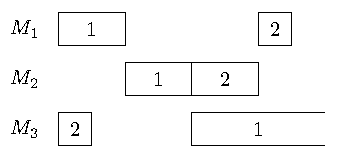
\includegraphics[scale=1]{figures/job-shop-delay.pdf}
  \caption{Example of an optimal schedule for Example~\ref{eg:job-shop}, shown
    as a Gantt chart. Each row $M_{i}$ corresponds to machine $i$ and each block
    numbered $j$ on this row represents the operation $(i,j)$. The dashed lines
    indicate unit time steps. Note that machine 2 is kept idle, while operation
    $(2,2)$ could have already been scheduled at time 1. Furthermore, for this
    particular instance, it can be checked that this is the unique optimal
    schedule.}
  \label{fig:job-shop-delay}
\end{figure}

\paragraph{Disjunctive graph.}

A commonly used representation of job shop problems is through their disjunctive
graph, which is a directed graph with vertices $\mathcal{N}$ corresponding to the
operations and two types of arcs.
%
The conjunctive arcs $\mathcal{C}$ are used to encode the predetermined machine
sequence of each job. Each such arc $(i, j) \rightarrow (k, j)$ encodes that job
$j$ should first be processed on machine $i$ before it is processed on machine
$k$.
%
When two distinct jobs $j_{1}$ and $j_{2}$ both require processing on the same
machine $i$, we say that they are conflicting.
%
The disjunctive arcs $\mathcal{D}$ are used to encode the possible choices of
resolving such conflicts, by deciding which of $j_{1}$ or $j_{2}$ visits $i$
first.
%
More specifically, let $j_{1}$ and $j_{2}$ be conflicting on some machine $i$,
then the nodes $(i,j_{1})$ and $(i,j_{2})$ are connected by two arcs in opposite
directions.

The disjunctive graph can also be used to encode (partial) solutions as follows.
%
It can be shown that each feasible solution corresponds to a selection
$\mathcal{O}$ of exactly one disjunctive arc from each pair such that the
induced graph $(\mathcal{N}, \mathcal{C} \cup \mathcal{O})$ is
acyclic~\cite{pinedoSchedulingTheoryAlgorithms2016}.
%
More precisely, consider two conflicting operations $(i,j_{1})$ and $(i,j_{2})$,
then $\mathcal{O}$ contains either $(i,j_{1}) \rightarrow (i,j_{2})$ or
$(i,j_{1}) \rightarrow (i,j_{2})$.
%
To illustrate this, the empty and complete disjunctive graphs for the instance
in Example~\ref{eg:job-shop} are shown in Figure~\ref{fig:disjunctive-graphs-job-shop}.

\begin{figure}
  \centering
  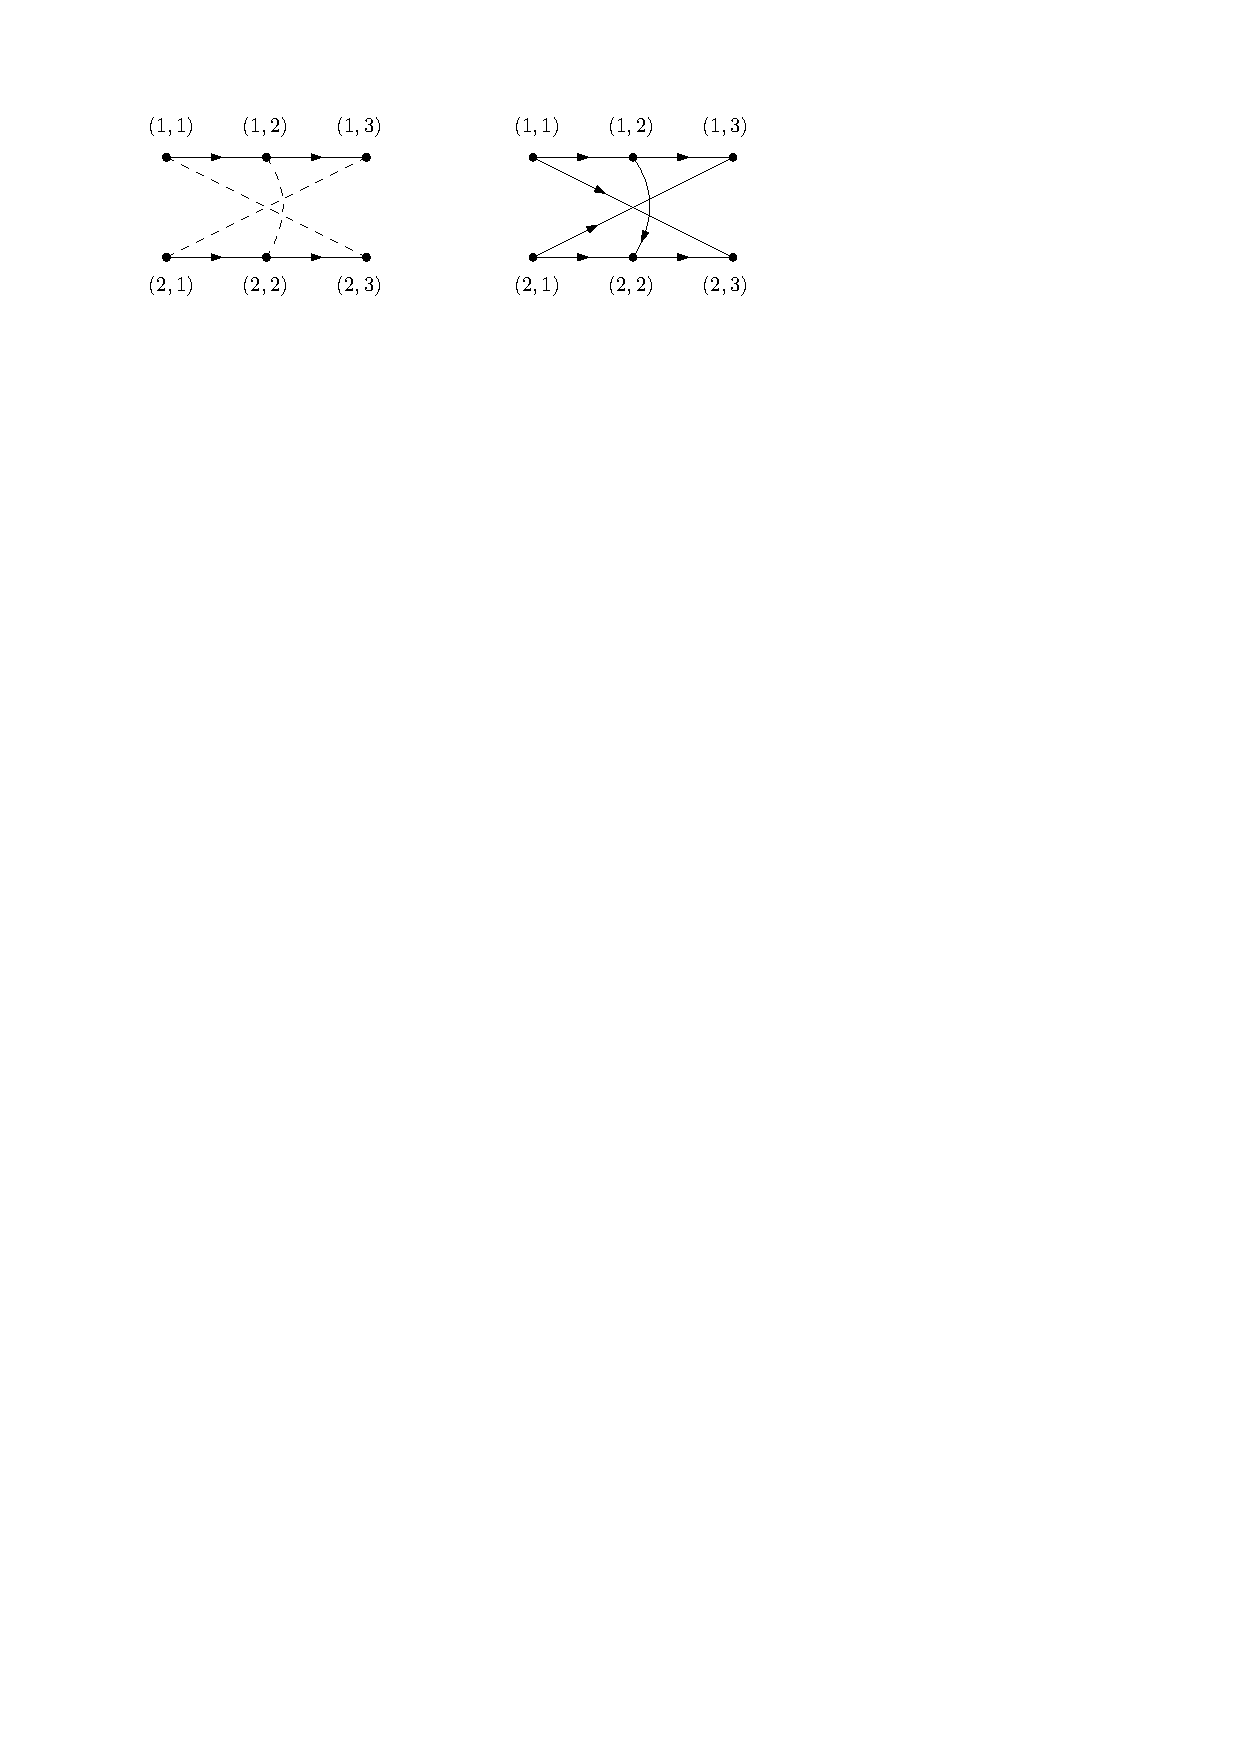
\includegraphics[scale=1]{figures/disjunctive_graph.pdf}
  \caption{Illustration of disjunctive graphs for Example~\ref{eg:job-shop}.
    Horizontal arrows represent conjunctive arcs. We used dashed lines to for
    the pairs of disjunctive arcs as dashed lines. The left graph corresponds to
    an empty selection $\mathcal{O} = \varnothing$ while the right graph shows
    the selection $\mathcal{O}$ that corresponds to the optimal schedule of
    Figure~\ref{fig:job-shop-delay}.}
  \label{fig:disjunctive-graphs-job-shop}
\end{figure}


\paragraph{Solution methods.}

Most job shop problems are very hard to solve. For example, the class of
problems $Jm|r_{j}|C_{\max}$ considered in Example~\ref{eg:job-shop} is known to
be NP-hard~\cite{grahamOptimizationApproximationDeterministic1979}, even without
release dates, which is denoted $Jm||C_{\max}$.
%
As a consequence, much effort has gone into developing good heurstics.
%
A type of heuristic that is often considered is to apply a so-called \emph{dispatching
rule} in order to build a schedule in a step-by-step fashion.
%
At each step, the rule chooses some job from all jobs with remaining unscheduled
operations and schedules this next operation at the earliest time possible,
given the current schedule.

A more principled way of solving job shop problems relies on the mathematical
programming framework.
%
We illustrate this for the problem $Jm|r_{j}|C_{\max}$ of
Example~\ref{eg:job-shop}. Using the notation of the disjunctive graph, the
problem can be concisely stated as
\[
\renewcommand{\arraystretch}{1.2}
\begin{NiceArray}{ r l @{} >{{}}c<{{}} @{} l @{} }
  \displaystyle \min_{y} & J(y) \\
  \text{such that } \; & y(s_{j},j) \leq r(j) && \quad \text{ for each job } j , \\
  &y(i, j) + p(i, j) \leq y(r, k) && \quad \text{ for each conjunction } (i,j) \rightarrow (r,k) \in \mathcal{C} , \\
  & y(i,j) + p(i,j) \leq y(i,k) & \\
  & \hspace{2em} \text{ or (not both) } && \quad \text{ for each disjunction } (i,j) \leftrightarrow (i,k) \in \mathcal{D} , \\
  & y(i,k) + p(i,k) \leq y(i,j) \\
  & y(i,j) \in \mathbb{R} && \quad \text{ for each operation } (i,j) \in \mathcal{N} .
\CodeAfter\SubMatrix.{4-1}{6-2}\}
\end{NiceArray}
\]
%
Note that this is almost an mixed-integer linear program (MILP).
%
Let $M > 0$ be some sufficiently large number and introduce a binary decision
variable $b_{(i,j)\leftrightarrow (i,k)} \in \{0,1\}$ for each pair of
disjunctive arcs, then the pair of disjunctive constraint can be rewritten to
\begin{align*}
  y(i,j) + p(i,j) &\leq y(i,k) + M b_{(i,j)\leftrightarrow (i,k)} , \\
  y(i,k) + p(i,k) &\leq y(i,j) + M (1 - b_{(i,j)\leftrightarrow (i,k)}) ,
\end{align*}
which is generally referred to as the \emph{big-M method}. The resulting MILP can
be solved by any off-the-shelf solver.

\chapter{Local search}\label{sec:local_search}

Without relying on systematic search methods like branch-and-bound, an often
employed method is to use some kind of local search heuristic.
%
The main idea is that the solution space can be organized based on some measure
of similarity. From the current solution, we only move to a neighboring solution
if it has a better objective value.
%
Next, give an example of such a neighborhood.

As seen in the previous sections, vehicles of the same route occur mostly in
platoons. For example, consider for example the route order
$\eta = (0, 1, 1, 0, 0, 1, 1, 1, 0, 0)$. This example has 5 platoons of
consecutive vehicles from the same route. The second platoon consists of two
vehicles from route 1.
%In general, let $P(\eta)$ denote the total number of platoons in $\eta$.
The basic idea is to make little changes in these platoons by moving vehicles at
the start and end of a platoon to the previous and next platoon of the same
route.
%
More precisely, we define the following two types of modifications to a route
order. A \textit{right-shift} modification of platoon $i$ moves the last vehicle of this
platoon to the next platoon of this route. Similarly, a \textit{left-shift} modification
of platoon $i$ moves the first vehicle of this platoon to the previous platoon
of this route.
%
We construct the neighborhood of a solution by performing every possible
right-shift and left-shift with respect to every platoon in the route order. For
illustration purposes, we have listed a full neighborhood for some example route
order in Table~\ref{tab:local_search}.

Now using this definition of a neighborhood, we must specify how the search
procedure visits these candidates.
In each of the following variants, the value of each neighbor is always computed.
%
The most straightforward way is to select the single best candidate in the
neighborhood and then continue with this as the current solution and compute its
neighborhood. This procedure can be repeated for some fixed number of times.
Alternatively, we can select the $k$ best neighboring candidates and then
compute the combined neighborhood for all of them. Then in the next step, we
again select the $k$ best candidates in this combined neighborhood and repeat.
The latter variant is generally known as \textit{beam search}.

\newcommand*{\one}{{\color{blue}1}}%
\newcommand*{\zero}{{\color{red}0}}%

\begin{table}
  \caption{Local search neighborhood of route order
    $\eta = (\zero, \one, \one, \zero, \zero, \one, \one, \one, \zero, \zero)$
    based on the left-shift and right-shift operations applied to every
    ``platoon'' in the current order.}
\label{tab:local_search}
\begin{center}
\begin{tabular}{c|c|c}
  platoon id  & left-shift & right-shift \\
  1 &  & (\one, \one, \zero, \zero, \zero, \one, \one, \one, \zero, \zero) \\
  2 & (\one, \zero, \one, \zero, \zero, \one, \one, \one, \zero, \zero) & (\zero, \one, \zero, \zero, \one, \one, \one, \one, \zero, \zero) \\
  3 & (\zero, \zero, \one, \one, \zero, \one, \one, \one, \zero, \zero) & (\zero, \one, \one, \zero, \one, \one, \one, \zero, \zero, \zero) \\
  4 & (\zero, \one, \one, \one, \zero, \zero, \one, \one, \zero, \zero) & (\zero, \one, \one, \zero, \zero, \one, \one, \zero, \zero, \one) \\
  5 & (\zero, \one, \one, \zero, \zero, \zero, \one, \one, \one, \zero) &
\end{tabular}
\end{center}
\end{table}



\chapter{Neural combinatorial optimization}\label{app:nco}

% maybe discuss traditional epsilon-approximation schemes?
% argue that it takes a lot of expert knowledge about the problem structure to design these

This section introduces the idea of applying a Machine Learning (ML) perspective
on Combinatorial Optimization (CO) problems, which has gained a lot of
attention\footnote{Pun not intended: a lot of recent works rely on neural attention architectures.} recently. One of the key ideas in this line of research is to treat problem
instances as data points and to use machine learning methods to approximately
map them to corresponding optimal solutions~\cite{bengioMachineLearningCombinatorial2020}.

% learning assumptions:
% supervised learning (expert labels) vs reinforcement learning (experience)
\paragraph{Algorithm execution as MDPs.}
It is very natural to see the sequential decision-making process of any
optimization algorithm in terms of the Markov Decision Process (MDP) framework,
where the environment corresponds to the internal state of the algorithm. From
this perspective, two main learning regimes can be distinguished.
% imitiation learning
Methods like those based on the branch-and-bound framework are
often computationally too expensive for practical purposes, so \textit{learning
  to imitate} the decisions taken in these exact algorithms might provide us
with fast approximations. In this approach, the ML model's performance is
measured in terms of how similar the produced decisions are to the
demonstrations provided by the expert.
% reinforcement learning
On the other hand, some problems do not even allow efficient exact methods, so it is
interesting to study solution methods that \textit{learn from experience}. An
interesting feature of this direction is that it enables the algorithm to implicitly
learn to exploit the hidden structure of the problems we want to solve.

% neural combinatorial optimization
Because neural networks are commonly used as encoder in these ML models for CO,
we will refer to this new field as \textit{Neural Combinatorial Optimization} (NCO).
%
A wide range of classical combinatorial optimization problems has already been
considered in this framework, so we briefly discuss the taxonomy used in the
survey~\cite{mazyavkinaReinforcementLearningCombinatorial2020}.
% principal vs. joint approach
One distinguishing feature is whether existing off-the-shelf solvers are used or
not. On the one hand, \textit{principal} methods are based on a parameterized algorithm
that is tuned to directly map instances to solutions, while \textit{joint} methods
integrate with existing off-the-shelf solvers in some way (see the
survey~\cite{lodiLearningBranchingSurvey2017} on integration with the
branch-and-bound framework). An illustrative example of the latter category are
the use of ML models for the branching heuristic or the selection of cutting
planes in branch-and-cut algorithms~\cite{tangReinforcementLearningInteger2020}.
% principal - construction vs. improvement (guided search)
The class of principal methods can be further divided into \textit{construction}
heuristics, which produce complete solutions by repeatedly extending partial
solutions, and \textit{improvement} heuristics, which aim at iteratively improving the
current solution with some tunable search procedure.


% learning algorithms:
% REINFOCE with baseline
% Fitting the neural mapping is often done using policy gradient methods (with
% baseline), e.g., with the classical REINFORCE algorithm.

% constraints in differentiable models

\paragraph{Constraint satisfaction.}
A major challenge in NCO is constraint satisfaction. For example, solutions
produced by neural construction policies need to satisfy the constraints of the
original combinatorial problem. To this end, neural network components have been
designed whose outputs satisfy some specific type of constraint, for example
being a permutation of the input~\cite{vinyalsPointerNetworks2017a}. Constraints can also be enforced by
the factorization of the mapping into repeated application of some policy. For
example, in methods for the classical traveling salesman problem, a policy is
defined that repeatedly selects the next node to visit. The constraint that
nodes may only be visited once can be easily enforced by ignoring the visited
nodes and taking the argmax among the model's probabilities for unvisited nodes.

% encoders:
% standard multilayer perceptron networks are not suited to encode order
% pointer networks
% graph neural networks

% backpropagation through solution
Instead of enforcing constraints by developing some tailored model architecture,
like construction and improvement heuristics, general methodologies have
recently been explored for the problem of constraint satisfaction in neural
networks. For example, the DC3 framework~\cite{dontiDC3LearningMethod2021}
employs two differentiable processes, completion and correction, to solve any
violations of equality or inequality constraints, respectively. The more recent
HardNet framework~\cite{minHardConstrainedNeuralNetworks2024} uses a closed-form
projection to map to feasible solutions under affine constraints and relies on a
differentiable convex optimization solver (e.g.,
OptNet~\cite{amosOptNetDifferentiableOptimization2021a}) when general convex
constraints are considered.

\paragraph{Neural job shop scheduling}
% examples for job-shop scheduling
Various NCO methods have already been studied for the Job Shop Scheduling Problem
(JSSP) with makespan objective, for which we now highlight some works that
illustrate some of the above classes of methods. A lot of the policies used in
these works rely on some graph neural network architecture, which is why the
survey~\cite{smitGraphNeuralNetworks2024} provides an overview based on this distinguishing feature.

% Tassel (principal construction, naive environment)
\paragraph{Dispatching rules.}
A very natural approach to model JSSP in terms of an MDP is taken
in~\cite{tasselReinforcementLearningEnvironment2021}, where a dispatching
heuristic is defined in an environment based on discrete scheduling time steps.
%
Every available job corresponds to a valid action and there is a so-called No-Op
action to skip to the next time step. States are encoded by some manually
designed features. They consider the makespan objective by proposing a dense
reward based on how much idle time is introduced compared to the processing time
of the job that is dispatched.
%
In some situation, some action can be proved to be always optimal (``non-final
prioritization''), in which case the policy is forced to take this action.
Additionally, the authors design some rules for when the No-Op action is not
allowed in order to prevent unnecessary idling of machines.
%
The proposed method is evaluated on the widely used
Taillard~\cite{taillardBenchmarksBasicScheduling1993} and
Demirkol~\cite{DEMIRKOL1998137} benchmarks, for which performance is compared to
static dispatching rules and a constraint programming (CP) solver, which is
considered cutting-edge.

% exact start times follow from order
From a scheduling theory
perspective~\cite{pinedoSchedulingTheoryAlgorithms2016}, it can be shown that
optimal schedules are completely characterized by the order of operations for
regular objectives (non-decreasing functions of the completion times). The start
times are computed from this order by a so-called \textit{placement rule}, so
considering discrete time steps introduces unnecessary model redundancy.

% Zhang construction heuristic (principal construction, based on order)

The seminal ``Learning to Dispatch'' (L2D)
paper~\cite{zhangLearningDispatchJob2020} proposes a construction heuristic for
JSSP with makespan objective. Their method is based on a dispatching policy that
is parameterized in terms of a graph neural network encoding of the disjunctive
graph belonging to a partial solution. Again, each action corresponds to
choosing for which job the next operation is dispatched. The rewards are based
on how much the lower bound on the makespan changes between successive states.
They use a Graph Isomorphism Network (GIN) architecture to parameterize both an
actor and critic, which are trained using the Proximal Policy Optimization (PPO)
algorithm. Using the Taillard and Demirkol benchmarks, they show that their
model is able to generalize well to larger instances.
% problem with dispatching mechanism
As we already alluded to above, this way of modeling the environment is better
suited to JSSP with regular objectives, because it does not explicitly determine
starting times.
%
They use a dispatching mechanism based on finding the earliest starting time of
a job, even before already scheduled jobs, see their Figure 2. By doing this,
they introduce symmetry in the environment: after operations
$O_{11}, O_{21}, O_{31}$ have been scheduled, both action sequences
$O_{22}, O_{32}$ and $O_{32}, O_{22}$ lead to exactly the same state $S_5$ shown
in their Figure 2. In this particular example, this means that it is impossible
to have $O_{11} \rightarrow O_{22} \rightarrow O_{32}$. In general, it is not
clear whether the resulting restricted policy is still sufficiently powerful, in
the sense that an optimal operation order can always be constructed.

% Zhang improvement heuristic (principal improvement)

\paragraph{Guided local search.}
Recently, the authors of L2D investigated an improvement heuristic for
JSSP~\cite{zhangDeepReinforcementLearning2024} with makespan objective.
%
This method is based on selecting a solution within the well-known $N_5$
neighborhood, which has been used in previous local search heuristics.
%
It is still not clear whether their resulting policy is complete, in the sense
that any operation order can be achieved by a sequence of neighborhood moves.
%
The reward is defined in terms of how much the solution improves relative to the
best solution seen so far (the ``incumbent'' solution). The policy is
parameterized using a GIN architecture designed to capture the topological
ordering of operations encoded in the disjunctive graph of solutions. They
propose a custom $n$-step variant of the REINFORCE algorithm in order to deal
with the sparse reward signal and long trajectories.
%
To compute the starting times based on the operation order, they propose a
dynamic programming algorithm, in terms of a message-passing scheme, as a more
efficient alternative to the classical recursive critical path method.
%
Our proposal for efficiently updating the current starting time lower bounds in
partial solutions can also be understood as a similar message-passing scheme,
but where only some messages are necessary.

\paragraph{Joint method.}
% Tassel (joint with CP solver)
An example of a joint method is given
in~\cite{tasselEndEndReinforcementLearning2023}, where the environment is stated
in terms of a Constraint Programming (CP) formulation. This allows the method to
be trained using demonstration from an off-the-shelf CP solver.


\chapter{Reinforcement learning}

For machine learning problems where data-collection is restricted in some way,
the supervised learning paradigm, i.e., learning from labeled examples, is
sometimes no longer appropriate or feasible.
%
Very generally, the reinforcement learning paradigm can viewed as a
generalization of supervised learning in which the data collection and selection
process is not fixed anymore.
%
The classical perspective is that of an \emph{agent} that tries to maximize some
cumulative \emph{rewward} signal when interacting in some \emph{environment},
which is formalized by the Markov Decision Process (MDP) model.
%
We refer the reader to~\cite{suttonReinforcementLearningIntroduction2018} for the commonly cited textbook introduction to RL
from this perspective.

\paragraph{Problem definition.}
Consider finite sets of states $\mathcal{S}$ and actions $\mathcal{A}$.
%
Given some current state $s$, the agent sends some action $a$ to the
environment, upon which it responds by providing some scalar reward signal $r$
and transitions to state $s'$, which happens with probablity $p(s', r | s, a)$.
%
By fixing a policy $\pi$, which is a function $\pi(a|s)$ that gives the
probablity of the agent choosing action $a$ in state $s$, we obtain the induced
\emph{state Markov chain} with transition probabilities
%
\begin{align*}
  \mathrm{Pr}(s \rightarrow s') = \sum_{a} \sum_{r} \pi(a|s) p(s', r | s, a) .
\end{align*}
Given some initial state distribution $h(s)$, we sample $S_{0} \sim h(s)$ and
use $S_{0}, S_{1}, S_{2}, \dots$ to denote some sample trajectory.
%
Moreover, we can also consider a more fine-grained Markov chain by considering
the sequence of states, actions and rewards
\begin{align*}
  S_{0}, A_{1}, R_{1}, S_{1}, A_{2}, R_{2}, S_{2}, \dots ,
\end{align*}
in which which the state Markov chain is naturally embedded. Such a sample
trajectory is also referred to as an \emph{episode}.
%
Let the corresponding \emph{return} at step $t$ be
defined as
\begin{align*}
  G_{t} = \sum_{k=t+1}^{\infty} R_{k} .
\end{align*}
By marking a subset of states as being \emph{final states}, we can consider finite episodes
\begin{align*}
  S_{0}, A_{1}, R_{1}, S_{1}, A_{2}, R_{2}, S_{2}, \dots S_{N},
\end{align*}
by using the convention that final states return zero reward and transition to
themselves almost surely.
%
For finite episodes, the goal is to find a policy $\pi$ that maximizes the
expected return $\mathbb{E}[G_{0}]$.

\paragraph{Solution methods.}
Most classical methods to find such an optimal policy $\pi$ can be categorized
as either being value-based or policy-based.
%
Value-based can be generally understood as producing some estimate $v(s)$ for
the expected return $\mathbb{E}[G_{0} | S_{0} = s]$. The optimal policy is then
parameterized in terms of these estimates $v(s)$.
%
In contrast, policy-based methods use a more direct parameterization of the
policy space and often rely on some kind of gradient-based optimization.
Specifically, let $\pi_{\theta}$ be some policy with parameters $\theta$, then we aim to
apply the gradient descent updating
\begin{align*}
  \theta \leftarrow \theta - \alpha \nabla \mathbb{E} [ G_{0} ]
\end{align*}
where $\alpha$ is referred to as the learning rate.
%
However, in almost all interesting situations, it is infeasible to compute the
gradient directly.

\paragraph{Induced Markov chain.}
For some fixed policy $\pi$ and initial state distribution $h$, we consider the
underlying \textit{induced Markov chain} over states. Because we are working with finite
episodes, the induced state process is a Markov chain with absorbing states.
%
We want to analyze how often states are visited on average, over multiple episodes.
%
To better understand what \textit{on average} means here, imagine that we link
together separate episodes to create a regular Markov chain without absorbing
states, in the following way: from each final state, we introduce state
transitions to the initial states according to distribution $h$, see also
Figure~\ref{fig:episodic_MC}. Furthermore, we will write $S_{t}^{(i)}$ to denote
the state at step $t$ of episode $i$.

\begin{figure}[h]
  \centering
  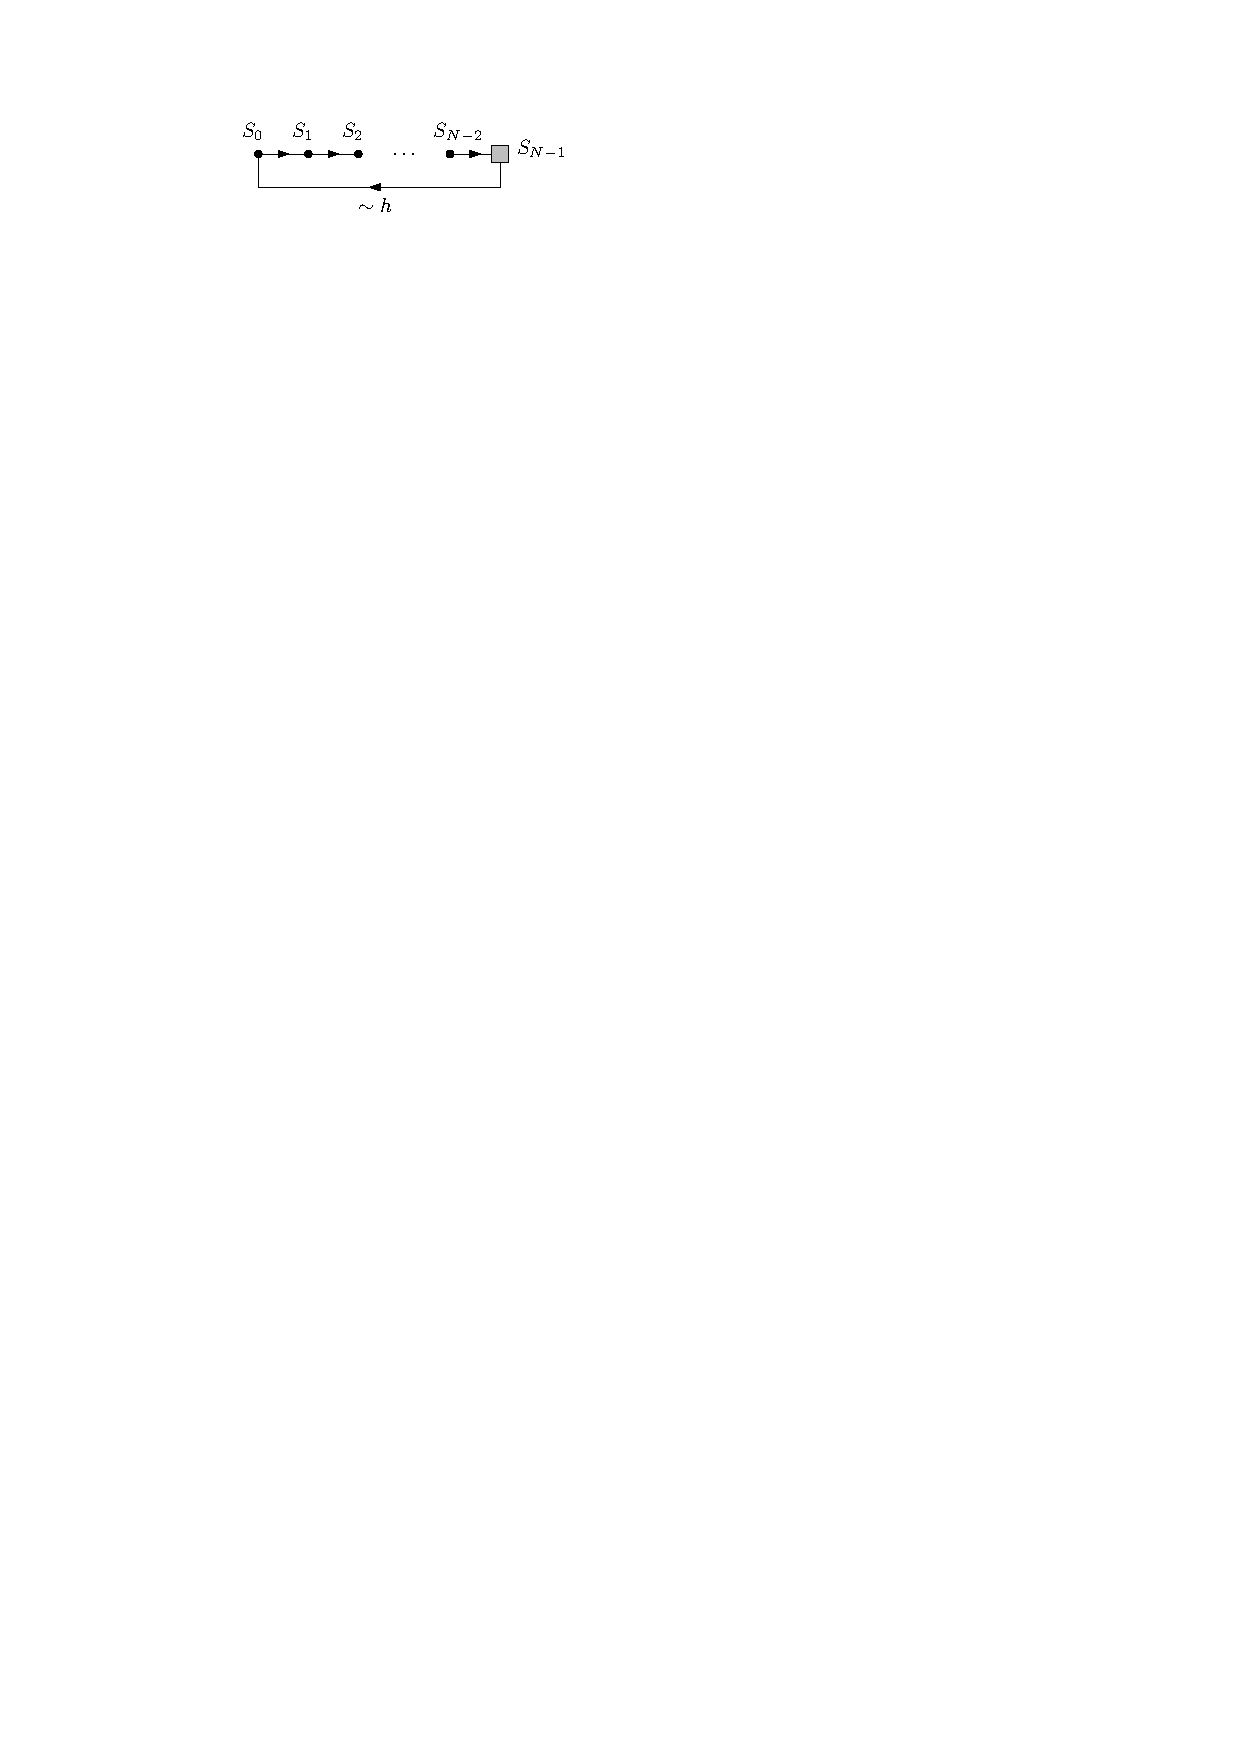
\includegraphics[width=0.4\textwidth]{figures/episodic_markov_chain.pdf}
  \caption{Illustration of the induced Markov chain when dealing with finite
    episodes. The next state after the final state, indicated as the grey
    rectangle, is sampled according to initial state distribution $h$.}
  \label{fig:episodic_MC}
\end{figure}


\section*{Stationary distribution for finite episodes}
Consider an absorbing Markov chain with transition matrix
\begin{align*}
  P_{xy} = \sum_{a} \pi(a | x) p(y | x, a) .
\end{align*}
There are $t$ transient states and $r$ absorbing states, so $P$ can be written
as
\begin{align*}
  P = \begin{pmatrix}
        Q & R \\
        \mathbf{0} & I_{r}
      \end{pmatrix} ,
\end{align*}
where $Q$ is a $t$-by-$t$ matrix, $R$ is a nonzero $t$-by-$r$ matrix, $I_{r}$ is
the $r$-by-$r$ identify matrix and $\mathbf{0}$ is the zero matrix.
%
Observe that $(Q^{k})_{xs}$ is the probability of reaching state $s$ in $k$
steps without being absorbed, starting from state $x$. Hence, the expected
number of visits to state $s$ without being absorbed, starting from state $x$,
is given by
\begin{align*}
  \eta(s | x) := \sum_{k=0}^{\infty} (Q^{k})_{xs} .
\end{align*}
%
Writing this in matrix form $N_{xs} = \eta(s | x)$, we can use the following
property of this so-called Neumann series, to obtain
\begin{align*}
  N = \sum_{k=0}^{\infty} Q^{k} = {(I_{t} - Q)}^{-1} .
\end{align*}
Now we can derive two equivalent equations
\begin{align*}
  N = (I_{t} - Q)^{-1} \iff
  \begin{cases}
    N (I_{t} - Q) = I_{t} \iff N = I_{t} + NQ ,
    \quad  \text{ or }  \\
    (I_{t} - Q) N = I_{t} \iff N = I_{t} + QN . \\
  \end{cases}
\end{align*}
%
Expanding the first equation in terms of matrix entries $N_{xs} = \eta(s | x)$
gives
\begin{align*}
  \eta(s | x) &= \mathds{1}\{ x = s \} + \sum_{y}  \eta(y | x) Q_{ys} \\
  &= \mathds{1}\{ x = s \} +  \sum_{y}\eta(y | x) \sum_{a} \pi(a | y) p(y | x, a)
\end{align*}
and similarly, the second equation gives
\begin{align*}
  \eta(s | x) &= \mathds{1}\{ x = s \} + \sum_{y} Q_{xy} \eta(s | y) \\
  &= \mathds{1}\{ x = s \} +  \sum_{a} \pi(a | x) \sum_{y} p(y | x, a) \eta(s | y)
\end{align*}
%
Now since the initial state is chosen according to distribution $h$, the
expected number of visits $\eta(s)$ to state $s$ in some episode is given by
\begin{align*}
  \eta(s) = \sum_{x} h(x) \eta(s | x) ,
\end{align*}
or written in matrix form $\eta = hN$, where $\eta$ and $h$ are row vectors.
%
Therefore, we can also work with the equations
\begin{align*}
  \begin{cases}
  hN = h + hNQ , \quad \text{ or } \\
  hN = h + hQN ,
  \end{cases}
\end{align*}
which are generally called \textit{balance equations}.
% or written in terms of matrix entries, respectively,
% \begin{align*}
%   \begin{cases}
%   \eta(s) = h(s) + \sum_{x} h(x) \sum_{y} \eta(y|x) \sum_{a} \pi(a|y)p(s|y, a) , \text{ or } \\
%   \eta(s) = h(s) + \sum_{x} h(x) \sum_{a} \pi(a | x) \sum_{y} p(y | x, a) \eta(s | y) .
%   \end{cases}
% \end{align*}
By writing the first variant as $\eta = h + \eta Q$ and expanding the matrix
multiplication, we obtain
\begin{align*}
  \eta(s) = h(s) + \sum_{y} \eta(y) \sum_{a} \pi(a|y)p(s|y,a) .
\end{align*}
%
Through appropriate normalization of the expected number of visits, we obtain
the average fraction of time spent in state $s$, given by
\begin{align*}
  \mu(s) = \frac{\eta(s)}{\sum_{s'} \eta(s')} .
\end{align*}

\paragraph{Sampling.}

Suppose we have some function $f : \mathcal{S} \rightarrow \mathbb{R}$ over
states and we are interested in estimating $\mathbb{E}_{S_{t}^{(i)} \sim \mu}[f(S_{t}^{(i)})]$.
%
We can just take random samples of $S_{t}^{(i)}$, by sampling initial state
$S_{0}^{(i)} \sim h$ and then \textit{rolling out} $\pi$ to obtain
\begin{align*}
\tau^{(i)} = (S_{0}^{(i)},A_{0}^{(i)},R_{1}^{(i)},S_{1}^{(i)},A_{1}^{(i)},R_{2}^{(i)},S_{2}^{(i)}, \dots, S_{N^{(i)}-1}^{(i)}) \sim \pi(\tau^{(i)} | S_{0}^{(i)}),
\end{align*}
where $N^{(i)}$ denotes the total number of states visited in this episode.
%
Given $M$ such episode samples, we compute the estimate as
\begin{align*}
  \mathbb{E}_{S_{t}^{(i)} \sim \mu} [ f(S_{t}^{(i)}) ] \approx \left( \sum_{i=1}^{M} \sum_{t=0}^{N^{(i)} - 1} f(S_{t}^{(i)}) \right) / \left( \sum_{i=1}^{M} N^{(i)} \right) .
\end{align*}

Observe that the analysis of the induced Markov chain can be extended to
explicitly include actions and rewards as part of the state and derive the
stationary distribution of the resulting Markov chain. However, we do not need
this distribution explicitly in practice, because we can again use episode
samples $\tau^{(i)}$. To keep notation concise, we will from now on denote this
type of expectation as $\mathbb{E}_{\tau \sim h,\pi}[f(\tau)]$ and omit episode
superscripts.
%
Using this new notation, note that the average episode length is given by
\begin{align*}
  \mathbb{E}_{h, \pi} [ N ]= \sum_{s'} \eta(s') .
\end{align*}

\section*{Policy gradient estimation}

Let $v_{\pi_{\theta}} = \mathbb{E}_{h,\pi_{\theta}}[G_{0}]$ denote the expected
episodic reward under policy $\pi$, where $G_{t}$ is called the reward-to-go at
step $t$, which is defined as
\begin{align*}
  G_{t} := \sum_{k=t+1}^{\infty} R_{k} .
\end{align*}
The main idea of policy gradient methods is to update the policy parameters
$\theta$ in the direction that increases the expected episodic reward the most. This
means that the policy parameters are updated as
\begin{align*}
  \theta_{k+1} = \theta_{k} + \alpha \nabla v_{\pi_{\theta}} ,
\end{align*}
where $\alpha$ is the learning rate and the gradient is with respect to
$\theta$. Instead of trying to derive or compute the gradient exactly, we often
use some statistical estimate based on sampled episode. The basic policy
gradient algorithm is to repeat the three steps

\vspace{1em}
\noindent
\hspace*{1em} \texttt{1. sample $M$ episodes $\tau^{(1)}, \dots, \tau^{(M)}$ following $\pi_{\theta}$,}\\
\hspace*{1em} \texttt{2. compute gradient estimate $\widehat{\nabla v_{\pi_{\theta}}}(\tau^{(1)}, \dots, \tau^{(M)})$,} \\
\hspace*{1em} \texttt{3. update $\theta \leftarrow \theta + \alpha \widehat{\nabla v_{\pi_{\theta}}}$.}

\paragraph{REINFORCE estimator.}

We will now present the fundamental policy gradient theorem, which essentially
provides a function $f$ such that
\begin{align*}
  \nabla v_{\pi_{\theta}} = \mathbb{E}_{\tau \sim h,\pi_{\theta}}[f(\tau)] ,
\end{align*}
which allows us to estimate the policy gradient using episode samples.
%
To align with the notation
of~\cite{suttonReinforcementLearningIntroduction2018}, we write
$\mathrm{Pr}(x \rightarrow s, k, \pi) := (Q^{k})_{xs}$, for the probability of
reaching state $s$ in $k$ steps under policy $\pi$, starting from state some
$x$, so that the expected number of visits can also be written as
\begin{align*}
  \eta(s) = \sum_{x} h(x) \sum_{k=0}^{\infty} \mathrm{Pr}(x \rightarrow s, k, \pi)
\end{align*}
%
As proven in the chapter on policy gradient methods
in~\cite{suttonReinforcementLearningIntroduction2018}, the gradient of the value
function for a fixed initial state $s_0$ with respect to the parameters is given
by
\begin{align}
  \nabla v_{\pi}(s_{0}) = \sum_{s} \sum_{k=0}^{\infty} \mathrm{Pr}(s_{0} \rightarrow s, k, \pi) \sum_{a} q_{\pi}(s,a) \nabla \pi(a|s) .
\end{align}
When choosing the initial state $s_{0}$ according to some distribution
$h(s_{0})$, we verify that the final result is still the same as in
\cite{suttonReinforcementLearningIntroduction2018}:
\begin{subequations}
\begin{align}
  \nabla v_{\pi} :=& \nabla \mathbb{E}_{s_{0} \sim h}[v_{\pi}(s_{0})] \\
  =& \sum_{s_{0}} h(s_{0}) \sum_{s} \sum_{k=0}^{\infty} \mathrm{Pr}(s_{0} \rightarrow s, k, \pi) \sum_{a} q_{\pi}(s,a) \nabla \pi(a|s) \\
  =& \sum_{s} \eta(s) \sum_{a} q_{\pi}(s,a) \nabla \pi(a|s) \\
  =& \sum_{s'} \eta(s') \sum_{s} \mu(s) \sum_{a} q_{\pi}(s,a) \nabla \pi(a|s) \\
  \propto& \sum_{s} \mu(s) \sum_{a} q_{\pi}(s,a) \nabla \pi(a|s) ,
\end{align}
\end{subequations}
where the constant of proportionality is just the average episode length.
%
Because we do not know $\mu$ or $q_{\pi}$ explicitly, we would like to estimate
$\nabla v_{\pi}$ based on samples. If we sample episodes according to $h$ and
$\pi$ as explained above, we encounter states according to $\mu$, so we have
\begin{subequations}
\begin{align}
  \nabla v_{\pi} &\propto \mathbb{E}_{h, \pi} \left[ \sum_{a} q_{\pi}(S_{t}, a) \nabla\pi(a | S_{t}) \right] \\
  &= \mathbb{E}_{h, \pi} \left[ \sum_{a} \pi(a | S_{t}) q_{\pi}(S_{t}, a) \frac{\nabla \pi(a | S_{t})}{\pi(a | S_{t})} \right] \\
  &= \mathbb{E}_{h, \pi} \left[ q_{\pi}(S_{t}, A_{t}) \frac{\nabla \pi(A_{t} | S_{t})}{\pi(A_{t}| S_{t})} \right] \\
  &= \mathbb{E}_{h, \pi} \left[ G_{t} \nabla \log \pi(A_{t} | S_{t}) \right] .
  \label{eq:estimator1}
\end{align}
\end{subequations}

\paragraph{Baseline.}
Let $b(s)$ be some function of the state $s$ only, then we have for any $s \in \mathcal{S}$
\begin{align}
  \sum_{a} b(s) \nabla \pi(a | s) = b(s) \nabla \sum_{a} \pi(a | s) = b(s) \nabla 1 = 0 .
\end{align}
This yields the so-called REINFORCE estimate with \textit{baseline}
\begin{subequations}
\begin{align}
  \nabla v_{\pi} &\propto \sum_{s} \mu(s) \sum_{a} (q_{\pi}(s, a) + b(s)) \nabla \pi(a | s) \\
          &= \mathbb{E}_{h, \pi} \left[ \bigl(q_{\pi}(S_{t}, A_{t}) + b(S_{t}) \bigr) \nabla \log \pi(A_{t} | S_{t}) \right] \\
  &= \mathbb{E}_{h, \pi} \left[ \bigl(G_{t} + b(S_{t}) \bigr) \nabla \log \pi(A_{t} | S_{t}) \right] .
  \label{eq:estimator2}
          %&= \mathbb{E}_{h, \pi} \left[ \bigl(G_{t} + b(S_{t}) \bigr) \nabla \log \pi(A_{t} | S_{t}) \right]
\end{align}
\end{subequations}
%
Although estimates~\eqref{eq:estimator1} and~\eqref{eq:estimator2} are both equivalent in terms of their expected
value, they may differ in higher moments, which is why an appropriate choice of
$b$ can make a lot of difference in how well the policy gradient algorithm
converges to an optimal policy.
%
As a specific baseline, consider the expected cumulative sum of rewards up to
step the current step $t$, defined as
\begin{align}
  b(s) = \mathbb{E}_{h,\pi} \left[ \sum_{k=1}^{t} R_{k} \Big| S_{t} = s \right],
\end{align}
then observe that
\begin{subequations}
\begin{align}
  q_{\pi}(s, a) + b(s) &= \mathbb{E}_{h,\pi}\left[ \sum_{k=t+1}^{\infty} R_{k} \Big| S_{t} = s , A_{t} = a \right] + \mathbb{E}_{h,\pi}\left[ \sum_{k=1}^{t} R_{k} \Big| S_{t} = s \right] \\
                     &= \mathbb{E}_{h,\pi}\left[ \sum_{k=1}^{\infty}  R_{k} \Big| S_{t} = s, A_{t} = a \right] \\
                     &= \mathbb{E}_{h,\pi} [ G_{0} | S_{t} = s, A_{t} = a ] ,
\end{align}
\end{subequations}
which is just the expected total episodic reward.
%
Now define function $f$ to be
\begin{subequations}
\begin{align}
  f(s, a) := (q_{\pi}(s, a) + b(s))\nabla \log \pi(a | s) &= \mathbb{E}_{h,\pi} \left[ G_{0} | S_{t} = s, A_{t} = a \right] \nabla \log \pi(a | s) \\
  &= \mathbb{E}_{h,\pi} \left[ G_{0} \nabla \log \pi(a | s) | S_{t} = s, A_{t} = a \right] ,
\end{align}
\end{subequations}
then applying the law of total expectation yields
\begin{align}
  \nabla v_{\pi} \propto \mathbb{E}_{h,\pi}[f(S_{t}, A_{t})] =  \mathbb{E}_{h, \pi} \left[ G_{0} \nabla \log \pi(A_{t} | S_{t}) \right] .
\end{align}


\chapter{Miscellaneous}\label{app:misc}

\minimalnode*
\begin{proof}
  For sake of contradiction, suppose there is no such minimal node, so every
  $v \in V$ has an incoming arc. Pick some arbitrary $v_0 \in V$, then there
  must exist $v_1 \in V$ such that $v_1 \rightarrow v_0$. Again, $v_1$ must have
  an incoming, so we can pick $v_2 \in V$ such that $v_2 \rightarrow v_1$. We
  can continue picking such predecessor as long as we want, obtaining a sequence
  $v_0, v_1, \dots, v_n$. Since there are only finitely many nodes, if we take
  the length $n$ of this sequence large enough, we must eventually pick a node
  twice, say $v_k = v_m$ for some $m < k \leq n$, but then we have
  $v_k \rightarrow v_{k-1} \rightarrow \cdots \rightarrow v_m = v_k$, which
  shows $\mathcal{G}$ has a cycle.

  To show that $\mathcal{G}$ has a topological order, consider the following
  procedure. Starting with $\mathcal{G}_0 := \mathcal{G}$ we select some minimal
  node $v_1$. We remove $v_1$ and all its outgoing edges from the graph to
  obtain a new graph $\mathcal{G}_1$, which is still a DAG, so there must be
  some minimal node $v_2$. We can repeat this procedure until
  $\mathcal{G}_{N}$ is an empty graph to obtain a sequence $v_1, \dots, v_N$.
  Suppose $v_i \rightarrow v_j$ in $\mathcal{G}$, then $v_i$ must appear earlier
  in the sequence than $v_j$, because otherwise $v_i$ was not a minimal element
  at the time it was picked.
\end{proof}


\begin{lemma}\label{lemma:inf-continuous}
  Let $f : X \times Y \rightarrow \mathbb{R}$ be some continuous function. If
  $Y$ is compact, then the function $g : X \rightarrow \mathbb{R}$, defined as
  $g(x) = \inf \{ f(x,y) : y\in Y\}$, is also continuous.
\end{lemma}

\begin{lemma}\label{lemma:levelset}
  Let $f :\mathbb{R}^{n} \rightarrow \mathbb{R}^{m}$ be continuous and
  $y \in \mathbb{R}^{m}$, then the level set $N := f^{-1}(\{ y \})$ is a closed
  subset of $\mathbb{R}^{n}$.
\end{lemma}
\begin{proof}
  For any $y' \neq y$, there exists an open neighborhood $M(y')$ such that
  $y \notin M(y')$. The preimage $f^{-1}(M(y'))$ is open by continuity.
  Therefore, the complement
  $N^{c} = \{ x : f(x) \neq y \} = \cup_{y' \neq y} f^{-1}(\{y'\}) = \cup_{y' \neq y} f^{-1}(M(y'))$
  is open.
\end{proof}


\note{The following definition might be helpful in deriving the buffer constraint.\dots}

\paragraph{Acceleration boundary.}
Before we present the decomposition, we first define an auxiliary upper
boundary.
%
Similar to how we generalized the entry boundary $\check{x}$ to the deceleration
boundary in Section~\ref{sec:deceleration-boundary}, we now generalize the exit
boundary $\hat{x}$ to obtain the \emph{acceleration boundary}.
%
Because the derivation is completely analogous, we will only present the
resulting expressions.
%
Let $x \in \mathcal{D}[a,b]$ be some smooth trajectory, then the acceleration
boundary $x^{+}[\xi]$ of $x$ at some $\xi \in [a,b]$ is defined as the
right-hand side of the inequality
\begin{align}
  x(t) \leq x(\xi) + \int_{\xi}^{t} \{\dot{x}(\xi) + \bar{\omega} (\tau - \xi) \}_{[0,1]} \diff \tau =: x^{+}[\xi](t) ,
\end{align}
which holds for every $t \in [a,b]$.
%
Observe that the exit boundary can now be written as the restricted acceleration
boundary $\hat{x} = (x^{+}[b])|_{[a,b]}$.
%
Similar to definition~\eqref{eq:def-x-}, we define
\begin{align}
  x^{+}[p,v,\xi](t) := p + \int_{\xi}^{t}\{ v + \bar{\omega}(\tau - \xi)\}_{[0,1]} \diff \tau ,
\end{align}
such that $x^{+}[\xi](t) = x^{+}[x(\xi),\dot{x}(\xi),\xi](t)$ and
%
similar to~\eqref{eq:x-}, we calculate
\begin{align}
  x^{+}[p,v,\xi](t) = p +
  \begin{cases}
    \dots &\text{ for } t \leq \bar{\delta}_{0} , \\
    \dots &\text{ for } t \in [\bar{\delta}_{0}, \bar{\delta}_{1} ] , \\
    \dots &\text{ for } t \geq \bar{\delta}_{1} ,
  \end{cases}
\end{align}
with $\bar{\delta}_{0} := $ and $\bar{\delta}_{1} := $.

\note{
Recall the definition of $\hat{x}$ in equation~\eqref{eq:hat-x}. By carefully
handling the $\max\{\cdot\}$, we can expand this expression as
\begin{align}
  \hat{x}(t) =
  \begin{cases}
    B - b + t + \bar{\omega} (b-t)^{2} / 2 &\text{ for } t \geq b - 1/\bar{\omega} , \\
    B - 1/(2\bar{\omega}) &\text{ for } t \leq b - 1/\bar{\omega} .
  \end{cases}
\end{align}
}

\newpage

\begin{restatable}{lemma}{lblemma}\label{lemma:lb-computation}
  Let $\mathcal{O}$ be some complete and acyclic selection, with unique vehicle
  order $\nu$, see~\Cref{rem:partial-order}. Suppose that $\sigma > \rho > 0$,
  then active schedule $y(\nu)$ is uniquely defined by starting with
  $y_{\nu_1} \leftarrow a_{\nu_1}$ and further following the recursion
\begin{align}
  \label{eq:lb-computation}
  y_{j} \leftarrow \max \{ a_{j}, y_i + w(i, j) \} ,
\end{align}
for every pair $i = \nu_t$ and $j = \nu_{t+1}$ with $t = 1, \dots, N-1$.
\end{restatable}
\begin{proof}
  We prove that $y$ obtained in this way is a feasible solution to~\eqref{eq:active_schedule} by
  showing that it satisfies~\eqref{eq:feasible-schedule}.
  %
  First of all, since $\nu_1$ is a minimal node of $G(\mathcal{O})$, we have
  $\mathcal{N}^-(\nu_1) = \varnothing$, so feasibility condition~\eqref{eq:feasible-schedule} is trivially satisfied
  with equality for $y_{\nu_1} = a_{\nu_1}$. We proceed inductively, by showing that,
  for any further $i = \nu_t$ and $j = \nu_{t+1}$, we have
  \begin{align}
    \label{eq:max-arc}
    y_i + w(i,j) = \max_{v \in \mathcal{N}^-(j)} y_v + w(v,j) ,
  \end{align}
  so that the definition of $y_j$ through~\eqref{eq:lb-computation} also
  satisfies~\eqref{eq:feasible-schedule} with equality.
  %
  Hence, uniqueness of $y$ simply follows from the fact that $y_j$
  satisfies~\eqref{eq:feasible-schedule} with equality for every $j \in \mathcal{N}$.

  For the inductive step, we simply verify that
  $y_{i} + w(i,j) \geq y_{v} + w(v,j)$ for any $v \in \mathcal{N}^{-}(j) \setminus \{i\}$, in
  each of the cases illustrated in Figure~\ref{fig:lb-computation}.
  %
  Suppose $i$ and $j$ are connected by $(i,j) \in \mathcal{C}$, then any other
  in-neighbor $v \in \mathcal{N}^-(j) \setminus \{ i \}$ must belong to a different route,
  so that $(v,j) \in \mathcal{O}$. Because $i$ and $j$ are on the same route and
  $i$ is the immediate predecessor of $j$ in the topological order, we must also
  have $(v,i) \in \mathcal{O}$. Therefore, we have
  \begin{align*}
    y_i + w(i,j) = y_i + \rho \geq y_v + \sigma + \rho > y_v + \sigma = y_v + w(v,j) .
  \end{align*}
  %
  Otherwise, $i$ and $j$ are connected by some disjunctive arc
  $(i,j) \in \mathcal{O}$. Let $v \in \mathcal{N}^-(j) \setminus \{i\}$, then if $v$ is on the
  same route as $j$, they are connected by a conjunctive arc
  $(v,j) \in \mathcal{C}$, so we must have $(v,i) \in \mathcal{O}$, again because
  $i$ is the immediate predecessor of $j$. Hence, we have
  \begin{align*}
    y_i + w(i,j) = y_i + \sigma \geq y_v + 2 \sigma > y_{v} + \rho = y_{v} + w(v,j) .
  \end{align*}
  %
  If $(v, j) \in \mathcal{O}$ with $r(v) \neq r(i)$, then it follows that
  $(v,i) \in \mathcal{O}$, so that
  \begin{align*}
    y_{i} + w(i,j) = y_i + \sigma \geq y_v + 2\sigma > y_v + \sigma = y_v + w(v,j) .
  \end{align*}
  If $(v, j) \in \mathcal{O}$ with $r(v) = r(i)$, then there is a path of
  conjunctive arcs between $v$ and $i$, from which it follows that
  $y_i \geq y_{v} + \rho$, so that
  \begin{align*}
    y_i + w(i,j) = y_i + \sigma \geq y_v + \sigma + \rho > y_v + w(v, j) . & \qedhere
  \end{align*}
\end{proof}


\begin{figure}
  \centering
  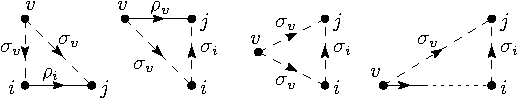
\includegraphics[width=0.8\textwidth]{figures/single/lower-bound-lemma.pdf}
  \caption{Sketch of the four cases distinguished in the proof of Lemma~\ref{lemma:lb-computation}. Arc
    weights are indicated by $\sigma$ and $\rho$. Conjunctive arcs $\mathcal{C}$ are
    drawn with solid lines and disjunctive arcs $\mathcal{O}$ are drawn with
    dashed lines. The dotted line depicts a chain of conjunctive arcs.}\label{fig:lb-computation}
\end{figure}

\end{document}

% add extra flag when compiling from emacs
% Local Variables:
% TeX-command-extra-options: "-shell-escape"
% End:
